\documentclass[twoside]{book}

% Packages required by doxygen
\usepackage{fixltx2e}
\usepackage{calc}
\usepackage{doxygen}
\usepackage[export]{adjustbox} % also loads graphicx
\usepackage{graphicx}
\usepackage[utf8]{inputenc}
\usepackage{makeidx}
\usepackage{multicol}
\usepackage{multirow}
\PassOptionsToPackage{warn}{textcomp}
\usepackage{textcomp}
\usepackage[nointegrals]{wasysym}
\usepackage[table]{xcolor}

% Font selection
\usepackage[T1]{fontenc}
\usepackage[scaled=.90]{helvet}
\usepackage{courier}
\usepackage{amssymb}
\usepackage{sectsty}
\renewcommand{\familydefault}{\sfdefault}
\allsectionsfont{%
  \fontseries{bc}\selectfont%
  \color{darkgray}%
}
\renewcommand{\DoxyLabelFont}{%
  \fontseries{bc}\selectfont%
  \color{darkgray}%
}
\newcommand{\+}{\discretionary{\mbox{\scriptsize$\hookleftarrow$}}{}{}}

% Page & text layout
\usepackage{geometry}
\geometry{%
  a4paper,%
  top=2.5cm,%
  bottom=2.5cm,%
  left=2.5cm,%
  right=2.5cm%
}
\tolerance=750
\hfuzz=15pt
\hbadness=750
\setlength{\emergencystretch}{15pt}
\setlength{\parindent}{0cm}
\setlength{\parskip}{3ex plus 2ex minus 2ex}
\makeatletter
\renewcommand{\paragraph}{%
  \@startsection{paragraph}{4}{0ex}{-1.0ex}{1.0ex}{%
    \normalfont\normalsize\bfseries\SS@parafont%
  }%
}
\renewcommand{\subparagraph}{%
  \@startsection{subparagraph}{5}{0ex}{-1.0ex}{1.0ex}{%
    \normalfont\normalsize\bfseries\SS@subparafont%
  }%
}
\makeatother

% Headers & footers
\usepackage{fancyhdr}
\pagestyle{fancyplain}
\fancyhead[LE]{\fancyplain{}{\bfseries\thepage}}
\fancyhead[CE]{\fancyplain{}{}}
\fancyhead[RE]{\fancyplain{}{\bfseries\leftmark}}
\fancyhead[LO]{\fancyplain{}{\bfseries\rightmark}}
\fancyhead[CO]{\fancyplain{}{}}
\fancyhead[RO]{\fancyplain{}{\bfseries\thepage}}
\fancyfoot[LE]{\fancyplain{}{}}
\fancyfoot[CE]{\fancyplain{}{}}
\fancyfoot[RE]{\fancyplain{}{\bfseries\scriptsize Generated by Doxygen }}
\fancyfoot[LO]{\fancyplain{}{\bfseries\scriptsize Generated by Doxygen }}
\fancyfoot[CO]{\fancyplain{}{}}
\fancyfoot[RO]{\fancyplain{}{}}
\renewcommand{\footrulewidth}{0.4pt}
\renewcommand{\chaptermark}[1]{%
  \markboth{#1}{}%
}
\renewcommand{\sectionmark}[1]{%
  \markright{\thesection\ #1}%
}

% Indices & bibliography
\usepackage{natbib}
\usepackage[titles]{tocloft}
\setcounter{tocdepth}{3}
\setcounter{secnumdepth}{5}
\makeindex

% Hyperlinks (required, but should be loaded last)
\usepackage{ifpdf}
\ifpdf
  \usepackage[pdftex,pagebackref=true]{hyperref}
\else
  \usepackage[ps2pdf,pagebackref=true]{hyperref}
\fi
\hypersetup{%
  colorlinks=true,%
  linkcolor=blue,%
  citecolor=blue,%
  unicode%
}

% Custom commands
\newcommand{\clearemptydoublepage}{%
  \newpage{\pagestyle{empty}\cleardoublepage}%
}

\usepackage{caption}
\captionsetup{labelsep=space,justification=centering,font={bf},singlelinecheck=off,skip=4pt,position=top}

%===== C O N T E N T S =====

\begin{document}

% Titlepage & ToC
\hypersetup{pageanchor=false,
             bookmarksnumbered=true,
             pdfencoding=unicode
            }
\pagenumbering{alph}
\begin{titlepage}
\vspace*{7cm}
\begin{center}%
{\Large Popgen G\+UI }\\
\vspace*{1cm}
{\large Generated by Doxygen 1.8.12}\\
\end{center}
\end{titlepage}
\clearemptydoublepage
\pagenumbering{roman}
\tableofcontents
\clearemptydoublepage
\pagenumbering{arabic}
\hypersetup{pageanchor=true}

%--- Begin generated contents ---
\chapter{Namespace Index}
\section{Namespace List}
Here is a list of all documented namespaces with brief descriptions\+:\begin{DoxyCompactList}
\item\contentsline{section}{\hyperlink{namespacenegui_1_1apgoperation}{negui.\+apgoperation} }{\pageref{namespacenegui_1_1apgoperation}}{}
\item\contentsline{section}{\hyperlink{namespacenegui_1_1createtooltip}{negui.\+createtooltip} }{\pageref{namespacenegui_1_1createtooltip}}{}
\item\contentsline{section}{\hyperlink{namespacenegui_1_1genepopfilemanager}{negui.\+genepopfilemanager} }{\pageref{namespacenegui_1_1genepopfilemanager}}{}
\item\contentsline{section}{\hyperlink{namespacenegui_1_1genepopfilesampler}{negui.\+genepopfilesampler} }{\pageref{namespacenegui_1_1genepopfilesampler}}{}
\item\contentsline{section}{\hyperlink{namespacenegui_1_1indiv}{negui.\+indiv} }{\pageref{namespacenegui_1_1indiv}}{}
\item\contentsline{section}{\hyperlink{namespacenegui_1_1negui}{negui.\+negui} }{\pageref{namespacenegui_1_1negui}}{}
\item\contentsline{section}{\hyperlink{namespacenegui_1_1pgdriveneestimator}{negui.\+pgdriveneestimator} }{\pageref{namespacenegui_1_1pgdriveneestimator}}{}
\item\contentsline{section}{\hyperlink{namespacenegui_1_1pgguiapp}{negui.\+pgguiapp} }{\pageref{namespacenegui_1_1pgguiapp}}{}
\item\contentsline{section}{\hyperlink{namespacenegui_1_1pgguisimupop}{negui.\+pgguisimupop} }{\pageref{namespacenegui_1_1pgguisimupop}}{}
\item\contentsline{section}{\hyperlink{namespacenegui_1_1pgguiutilities}{negui.\+pgguiutilities} }{\pageref{namespacenegui_1_1pgguiutilities}}{}
\item\contentsline{section}{\hyperlink{namespacenegui_1_1pghostnotebook}{negui.\+pghostnotebook} }{\pageref{namespacenegui_1_1pghostnotebook}}{}
\item\contentsline{section}{\hyperlink{namespacenegui_1_1pginputneestimator}{negui.\+pginputneestimator} }{\pageref{namespacenegui_1_1pginputneestimator}}{}
\item\contentsline{section}{\hyperlink{namespacenegui_1_1pginputsimupop}{negui.\+pginputsimupop} }{\pageref{namespacenegui_1_1pginputsimupop}}{}
\item\contentsline{section}{\hyperlink{namespacenegui_1_1pgmenubuilder}{negui.\+pgmenubuilder} }{\pageref{namespacenegui_1_1pgmenubuilder}}{}
\item\contentsline{section}{\hyperlink{namespacenegui_1_1pgopneestimator}{negui.\+pgopneestimator} }{\pageref{namespacenegui_1_1pgopneestimator}}{}
\item\contentsline{section}{\hyperlink{namespacenegui_1_1pgopsimupop}{negui.\+pgopsimupop} }{\pageref{namespacenegui_1_1pgopsimupop}}{}
\item\contentsline{section}{\hyperlink{namespacenegui_1_1pgoutputneestimator}{negui.\+pgoutputneestimator} }{\pageref{namespacenegui_1_1pgoutputneestimator}}{}
\item\contentsline{section}{\hyperlink{namespacenegui_1_1pgoutputsimupop}{negui.\+pgoutputsimupop} }{\pageref{namespacenegui_1_1pgoutputsimupop}}{}
\item\contentsline{section}{\hyperlink{namespacenegui_1_1pgparamset}{negui.\+pgparamset} }{\pageref{namespacenegui_1_1pgparamset}}{}
\item\contentsline{section}{\hyperlink{namespacenegui_1_1pgsimupopresources}{negui.\+pgsimupopresources} }{\pageref{namespacenegui_1_1pgsimupopresources}}{}
\item\contentsline{section}{\hyperlink{namespacenegui_1_1pgutilities}{negui.\+pgutilities} }{\pageref{namespacenegui_1_1pgutilities}}{}
\item\contentsline{section}{\hyperlink{namespacenegui_1_1pgutilityclasses}{negui.\+pgutilityclasses} }{\pageref{namespacenegui_1_1pgutilityclasses}}{}
\end{DoxyCompactList}

\chapter{Hierarchical Index}
\section{Class Hierarchy}
This inheritance list is sorted roughly, but not completely, alphabetically\+:\begin{DoxyCompactList}
\item A\+P\+G\+Operation\begin{DoxyCompactList}
\item \contentsline{section}{negui.\+pgopsimupop.\+P\+G\+Op\+Simu\+Pop}{\pageref{classnegui_1_1pgopsimupop_1_1PGOpSimuPop}}{}
\end{DoxyCompactList}
\item Frame\begin{DoxyCompactList}
\item \contentsline{section}{negui.\+pgguiapp.\+P\+G\+Gui\+App}{\pageref{classnegui_1_1pgguiapp_1_1PGGuiApp}}{}
\item \contentsline{section}{negui.\+pgguiutilities.\+Key\+Categorical\+Value\+Frame}{\pageref{classnegui_1_1pgguiutilities_1_1KeyCategoricalValueFrame}}{}
\item \contentsline{section}{negui.\+pgguiutilities.\+Key\+List\+Combo\+Frame}{\pageref{classnegui_1_1pgguiutilities_1_1KeyListComboFrame}}{}
\item \contentsline{section}{negui.\+pgguiutilities.\+Key\+Val\+Frame}{\pageref{classnegui_1_1pgguiutilities_1_1KeyValFrame}}{}
\item \contentsline{section}{negui.\+pgguiutilities.\+List\+Editing\+Subframe}{\pageref{classnegui_1_1pgguiutilities_1_1ListEditingSubframe}}{}
\end{DoxyCompactList}
\item Notebook\begin{DoxyCompactList}
\item \contentsline{section}{negui.\+pghostnotebook.\+P\+G\+Host\+Notebook}{\pageref{classnegui_1_1pghostnotebook_1_1PGHostNotebook}}{}
\end{DoxyCompactList}
\item object\begin{DoxyCompactList}
\item \contentsline{section}{negui.\+apgoperation.\+A\+P\+G\+Operation}{\pageref{classnegui_1_1apgoperation_1_1APGOperation}}{}
\item \contentsline{section}{negui.\+createtooltip.\+Create\+Tool\+Tip}{\pageref{classnegui_1_1createtooltip_1_1CreateToolTip}}{}
\item \contentsline{section}{negui.\+genepopfilemanager.\+Genepop\+File\+Manager}{\pageref{classnegui_1_1genepopfilemanager_1_1GenepopFileManager}}{}
\item \contentsline{section}{negui.\+genepopfilesampler.\+Genepop\+File\+Sample\+Params}{\pageref{classnegui_1_1genepopfilesampler_1_1GenepopFileSampleParams}}{}
\begin{DoxyCompactList}
\item \contentsline{section}{negui.\+genepopfilesampler.\+Genepop\+File\+Sample\+Params\+Age\+Structure\+Cohorts}{\pageref{classnegui_1_1genepopfilesampler_1_1GenepopFileSampleParamsAgeStructureCohorts}}{}
\item \contentsline{section}{negui.\+genepopfilesampler.\+Genepop\+File\+Sample\+Params\+Age\+Structure\+Relateds}{\pageref{classnegui_1_1genepopfilesampler_1_1GenepopFileSampleParamsAgeStructureRelateds}}{}
\item \contentsline{section}{negui.\+genepopfilesampler.\+Genepop\+File\+Sample\+Params\+Criteria}{\pageref{classnegui_1_1genepopfilesampler_1_1GenepopFileSampleParamsCriteria}}{}
\begin{DoxyCompactList}
\item \contentsline{section}{negui.\+genepopfilesampler.\+Genepop\+File\+Sample\+Params\+Criteria\+On\+Groups}{\pageref{classnegui_1_1genepopfilesampler_1_1GenepopFileSampleParamsCriteriaOnGroups}}{}
\end{DoxyCompactList}
\item \contentsline{section}{negui.\+genepopfilesampler.\+Genepop\+File\+Sample\+Params\+Loci}{\pageref{classnegui_1_1genepopfilesampler_1_1GenepopFileSampleParamsLoci}}{}
\item \contentsline{section}{negui.\+genepopfilesampler.\+Genepop\+File\+Sample\+Params\+None}{\pageref{classnegui_1_1genepopfilesampler_1_1GenepopFileSampleParamsNone}}{}
\item \contentsline{section}{negui.\+genepopfilesampler.\+Genepop\+File\+Sample\+Params\+Proportion}{\pageref{classnegui_1_1genepopfilesampler_1_1GenepopFileSampleParamsProportion}}{}
\item \contentsline{section}{negui.\+genepopfilesampler.\+Genepop\+File\+Sample\+Params\+Removal}{\pageref{classnegui_1_1genepopfilesampler_1_1GenepopFileSampleParamsRemoval}}{}
\end{DoxyCompactList}
\item \contentsline{section}{negui.\+genepopfilesampler.\+Genepop\+File\+Sampler}{\pageref{classnegui_1_1genepopfilesampler_1_1GenepopFileSampler}}{}
\begin{DoxyCompactList}
\item \contentsline{section}{negui.\+genepopfilesampler.\+Genepop\+File\+Sampler\+Individuals\+Age\+Structure\+Cohorts}{\pageref{classnegui_1_1genepopfilesampler_1_1GenepopFileSamplerIndividualsAgeStructureCohorts}}{}
\begin{DoxyCompactList}
\item \contentsline{section}{negui.\+genepopfilesampler.\+Genepop\+File\+Sampler\+Individuals\+Age\+Structure\+Cohorts\+Percentage}{\pageref{classnegui_1_1genepopfilesampler_1_1GenepopFileSamplerIndividualsAgeStructureCohortsPercentage}}{}
\end{DoxyCompactList}
\item \contentsline{section}{negui.\+genepopfilesampler.\+Genepop\+File\+Sampler\+Individuals\+Age\+Structure\+Relateds}{\pageref{classnegui_1_1genepopfilesampler_1_1GenepopFileSamplerIndividualsAgeStructureRelateds}}{}
\item \contentsline{section}{negui.\+genepopfilesampler.\+Genepop\+File\+Sampler\+Individuals\+By\+Criteria}{\pageref{classnegui_1_1genepopfilesampler_1_1GenepopFileSamplerIndividualsByCriteria}}{}
\item \contentsline{section}{negui.\+genepopfilesampler.\+Genepop\+File\+Sampler\+Individuals\+By\+Criteria\+Factored}{\pageref{classnegui_1_1genepopfilesampler_1_1GenepopFileSamplerIndividualsByCriteriaFactored}}{}
\item \contentsline{section}{negui.\+genepopfilesampler.\+Genepop\+File\+Sampler\+Individuals\+By\+Proportion}{\pageref{classnegui_1_1genepopfilesampler_1_1GenepopFileSamplerIndividualsByProportion}}{}
\item \contentsline{section}{negui.\+genepopfilesampler.\+Genepop\+File\+Sampler\+Individuals\+By\+Removal}{\pageref{classnegui_1_1genepopfilesampler_1_1GenepopFileSamplerIndividualsByRemoval}}{}
\item \contentsline{section}{negui.\+genepopfilesampler.\+Genepop\+File\+Sampler\+Loci\+By\+Range\+And\+Percentage}{\pageref{classnegui_1_1genepopfilesampler_1_1GenepopFileSamplerLociByRangeAndPercentage}}{}
\item \contentsline{section}{negui.\+genepopfilesampler.\+Genepop\+File\+Sampler\+Loci\+By\+Range\+And\+Total}{\pageref{classnegui_1_1genepopfilesampler_1_1GenepopFileSamplerLociByRangeAndTotal}}{}
\item \contentsline{section}{negui.\+genepopfilesampler.\+Genepop\+File\+Sampler\+None}{\pageref{classnegui_1_1genepopfilesampler_1_1GenepopFileSamplerNone}}{}
\end{DoxyCompactList}
\item \contentsline{section}{negui.\+genepopfilesampler.\+Genepop\+File\+Sampler\+Individuals\+By\+Criteria\+Grouped}{\pageref{classnegui_1_1genepopfilesampler_1_1GenepopFileSamplerIndividualsByCriteriaGrouped}}{}
\item \contentsline{section}{negui.\+genepopindividualid.\+Genepop\+Indiv\+Criteria}{\pageref{classnegui_1_1genepopindividualid_1_1GenepopIndivCriteria}}{}
\item \contentsline{section}{negui.\+genepopindividualid.\+Genepop\+Indiv\+Criterion}{\pageref{classnegui_1_1genepopindividualid_1_1GenepopIndivCriterion}}{}
\item \contentsline{section}{negui.\+genepopindividualid.\+Genepop\+Indiv\+Id\+Age\+Structure}{\pageref{classnegui_1_1genepopindividualid_1_1GenepopIndivIdAgeStructure}}{}
\item \contentsline{section}{negui.\+genepopindividualid.\+Genepop\+Indiv\+Id\+Fields}{\pageref{classnegui_1_1genepopindividualid_1_1GenepopIndivIdFields}}{}
\item \contentsline{section}{negui.\+genepopindividualid.\+Genepop\+Individual\+Id}{\pageref{classnegui_1_1genepopindividualid_1_1GenepopIndividualId}}{}
\item \contentsline{section}{negui.\+genepopindividualid.\+Genepop\+Indiv\+Id\+Vals}{\pageref{classnegui_1_1genepopindividualid_1_1GenepopIndivIdVals}}{}
\item \contentsline{section}{negui.\+pgdriveneestimator.\+Debug\+Mode}{\pageref{classnegui_1_1pgdriveneestimator_1_1DebugMode}}{}
\item \contentsline{section}{negui.\+pgguiutilities.\+Frame\+Container\+Scrolled}{\pageref{classnegui_1_1pgguiutilities_1_1FrameContainerScrolled}}{}
\item \contentsline{section}{negui.\+pgguiutilities.\+Frame\+Container\+V\+Scroll}{\pageref{classnegui_1_1pgguiutilities_1_1FrameContainerVScroll}}{}
\item \contentsline{section}{negui.\+pgguiutilities.\+P\+G\+G\+U\+I\+Error\+Message}{\pageref{classnegui_1_1pgguiutilities_1_1PGGUIErrorMessage}}{}
\item \contentsline{section}{negui.\+pgguiutilities.\+P\+G\+G\+U\+I\+Info\+Message}{\pageref{classnegui_1_1pgguiutilities_1_1PGGUIInfoMessage}}{}
\item \contentsline{section}{negui.\+pgguiutilities.\+P\+G\+G\+U\+I\+Message\+And\+Action\+On\+Cancel}{\pageref{classnegui_1_1pgguiutilities_1_1PGGUIMessageAndActionOnCancel}}{}
\item \contentsline{section}{negui.\+pgguiutilities.\+P\+G\+G\+U\+I\+Warning\+Message}{\pageref{classnegui_1_1pgguiutilities_1_1PGGUIWarningMessage}}{}
\item \contentsline{section}{negui.\+pgguiutilities.\+P\+G\+G\+U\+I\+Yes\+No\+Message}{\pageref{classnegui_1_1pgguiutilities_1_1PGGUIYesNoMessage}}{}
\item \contentsline{section}{negui.\+pginputneestimator.\+P\+G\+Input\+Ne\+Estimator}{\pageref{classnegui_1_1pginputneestimator_1_1PGInputNeEstimator}}{}
\item \contentsline{section}{negui.\+pginputsimupop.\+P\+G\+Input\+Simu\+Pop}{\pageref{classnegui_1_1pginputsimupop_1_1PGInputSimuPop}}{}
\item \contentsline{section}{negui.\+pgmenubuilder.\+P\+G\+Menu\+Builder}{\pageref{classnegui_1_1pgmenubuilder_1_1PGMenuBuilder}}{}
\item \contentsline{section}{negui.\+pgoutputneestimator.\+P\+G\+Output\+Ne\+Estimator}{\pageref{classnegui_1_1pgoutputneestimator_1_1PGOutputNeEstimator}}{}
\item \contentsline{section}{negui.\+pgoutputsimupop.\+P\+G\+Output\+Simu\+Pop}{\pageref{classnegui_1_1pgoutputsimupop_1_1PGOutputSimuPop}}{}
\item \contentsline{section}{negui.\+pgparamset.\+P\+G\+Param\+Set}{\pageref{classnegui_1_1pgparamset_1_1PGParamSet}}{}
\item \contentsline{section}{negui.\+pgsimupopresources.\+P\+G\+Simu\+Pop\+Resources}{\pageref{classnegui_1_1pgsimupopresources_1_1PGSimuPopResources}}{}
\item \contentsline{section}{negui.\+pgutilityclasses.\+Float\+Int\+String\+Param\+Validity}{\pageref{classnegui_1_1pgutilityclasses_1_1FloatIntStringParamValidity}}{}
\item \contentsline{section}{negui.\+pgutilityclasses.\+Independant\+Process\+Group}{\pageref{classnegui_1_1pgutilityclasses_1_1IndependantProcessGroup}}{}
\item \contentsline{section}{negui.\+pgutilityclasses.\+Independant\+Subprocess\+Group}{\pageref{classnegui_1_1pgutilityclasses_1_1IndependantSubprocessGroup}}{}
\item \contentsline{section}{negui.\+pgutilityclasses.\+Ne\+Estimator\+Sampling\+Scheme\+Parameter\+Manager}{\pageref{classnegui_1_1pgutilityclasses_1_1NeEstimatorSamplingSchemeParameterManager}}{}
\item \contentsline{section}{negui.\+pgutilityclasses.\+Value\+Validator}{\pageref{classnegui_1_1pgutilityclasses_1_1ValueValidator}}{}
\end{DoxyCompactList}
\item P\+G\+Gui\+App\begin{DoxyCompactList}
\item \contentsline{section}{negui.\+pgguineestimator.\+P\+G\+Gui\+Ne\+Estimator}{\pageref{classnegui_1_1pgguineestimator_1_1PGGuiNeEstimator}}{}
\item \contentsline{section}{negui.\+pgguisimupop.\+P\+G\+Gui\+Simu\+Pop}{\pageref{classnegui_1_1pgguisimupop_1_1PGGuiSimuPop}}{}
\end{DoxyCompactList}
\item Scrollbar\begin{DoxyCompactList}
\item \contentsline{section}{negui.\+pgguiutilities.\+Fred\+Lundhs\+Auto\+Scrollbar}{\pageref{classnegui_1_1pgguiutilities_1_1FredLundhsAutoScrollbar}}{}
\end{DoxyCompactList}
\item A\+P\+G\+Operation\begin{DoxyCompactList}
\item \contentsline{section}{negui.\+pgopneestimator.\+P\+G\+Op\+Ne\+Estimator}{\pageref{classnegui_1_1pgopneestimator_1_1PGOpNeEstimator}}{}
\end{DoxyCompactList}
\item Menu\begin{DoxyCompactList}
\item \contentsline{section}{negui.\+pgguiutilities.\+Right\+Click\+Menu}{\pageref{classnegui_1_1pgguiutilities_1_1RightClickMenu}}{}
\end{DoxyCompactList}
\end{DoxyCompactList}

\chapter{Class Index}
\section{Class List}
Here are the classes, structs, unions and interfaces with brief descriptions\+:\begin{DoxyCompactList}
\item\contentsline{section}{\hyperlink{classnegui_1_1apgoperation_1_1APGOperation}{negui.\+apgoperation.\+A\+P\+G\+Operation} }{\pageref{classnegui_1_1apgoperation_1_1APGOperation}}{}
\item\contentsline{section}{\hyperlink{classnegui_1_1pgdriveneestimator_1_1ArgSet}{negui.\+pgdriveneestimator.\+Arg\+Set} }{\pageref{classnegui_1_1pgdriveneestimator_1_1ArgSet}}{}
\item\contentsline{section}{\hyperlink{classnegui_1_1createtooltip_1_1CreateToolTip}{negui.\+createtooltip.\+Create\+Tool\+Tip} }{\pageref{classnegui_1_1createtooltip_1_1CreateToolTip}}{}
\item\contentsline{section}{\hyperlink{classnegui_1_1pgdriveneestimator_1_1DebugMode}{negui.\+pgdriveneestimator.\+Debug\+Mode} }{\pageref{classnegui_1_1pgdriveneestimator_1_1DebugMode}}{}
\item\contentsline{section}{\hyperlink{classnegui_1_1pgutilityclasses_1_1FloatIntStringParamValidity}{negui.\+pgutilityclasses.\+Float\+Int\+String\+Param\+Validity} }{\pageref{classnegui_1_1pgutilityclasses_1_1FloatIntStringParamValidity}}{}
\item\contentsline{section}{\hyperlink{classnegui_1_1pgguiutilities_1_1FrameContainerScrolled}{negui.\+pgguiutilities.\+Frame\+Container\+Scrolled} }{\pageref{classnegui_1_1pgguiutilities_1_1FrameContainerScrolled}}{}
\item\contentsline{section}{\hyperlink{classnegui_1_1pgguiutilities_1_1FrameContainerVScroll}{negui.\+pgguiutilities.\+Frame\+Container\+V\+Scroll} }{\pageref{classnegui_1_1pgguiutilities_1_1FrameContainerVScroll}}{}
\item\contentsline{section}{\hyperlink{classnegui_1_1pgguiutilities_1_1FredLundhsAutoScrollbar}{negui.\+pgguiutilities.\+Fred\+Lundhs\+Auto\+Scrollbar} }{\pageref{classnegui_1_1pgguiutilities_1_1FredLundhsAutoScrollbar}}{}
\item\contentsline{section}{\hyperlink{classnegui_1_1genepopfilemanager_1_1GenepopFileManager}{negui.\+genepopfilemanager.\+Genepop\+File\+Manager} }{\pageref{classnegui_1_1genepopfilemanager_1_1GenepopFileManager}}{}
\item\contentsline{section}{\hyperlink{classnegui_1_1genepopfilesampler_1_1GenepopFileSampleParams}{negui.\+genepopfilesampler.\+Genepop\+File\+Sample\+Params} }{\pageref{classnegui_1_1genepopfilesampler_1_1GenepopFileSampleParams}}{}
\item\contentsline{section}{\hyperlink{classnegui_1_1genepopfilesampler_1_1GenepopFileSampleParamsAgeStructureCohorts}{negui.\+genepopfilesampler.\+Genepop\+File\+Sample\+Params\+Age\+Structure\+Cohorts} }{\pageref{classnegui_1_1genepopfilesampler_1_1GenepopFileSampleParamsAgeStructureCohorts}}{}
\item\contentsline{section}{\hyperlink{classnegui_1_1genepopfilesampler_1_1GenepopFileSampleParamsAgeStructureRelateds}{negui.\+genepopfilesampler.\+Genepop\+File\+Sample\+Params\+Age\+Structure\+Relateds} }{\pageref{classnegui_1_1genepopfilesampler_1_1GenepopFileSampleParamsAgeStructureRelateds}}{}
\item\contentsline{section}{\hyperlink{classnegui_1_1genepopfilesampler_1_1GenepopFileSampleParamsCriteria}{negui.\+genepopfilesampler.\+Genepop\+File\+Sample\+Params\+Criteria} }{\pageref{classnegui_1_1genepopfilesampler_1_1GenepopFileSampleParamsCriteria}}{}
\item\contentsline{section}{\hyperlink{classnegui_1_1genepopfilesampler_1_1GenepopFileSampleParamsCriteriaOnGroups}{negui.\+genepopfilesampler.\+Genepop\+File\+Sample\+Params\+Criteria\+On\+Groups} }{\pageref{classnegui_1_1genepopfilesampler_1_1GenepopFileSampleParamsCriteriaOnGroups}}{}
\item\contentsline{section}{\hyperlink{classnegui_1_1genepopfilesampler_1_1GenepopFileSampleParamsLoci}{negui.\+genepopfilesampler.\+Genepop\+File\+Sample\+Params\+Loci} }{\pageref{classnegui_1_1genepopfilesampler_1_1GenepopFileSampleParamsLoci}}{}
\item\contentsline{section}{\hyperlink{classnegui_1_1genepopfilesampler_1_1GenepopFileSampleParamsNone}{negui.\+genepopfilesampler.\+Genepop\+File\+Sample\+Params\+None} }{\pageref{classnegui_1_1genepopfilesampler_1_1GenepopFileSampleParamsNone}}{}
\item\contentsline{section}{\hyperlink{classnegui_1_1genepopfilesampler_1_1GenepopFileSampleParamsProportion}{negui.\+genepopfilesampler.\+Genepop\+File\+Sample\+Params\+Proportion} }{\pageref{classnegui_1_1genepopfilesampler_1_1GenepopFileSampleParamsProportion}}{}
\item\contentsline{section}{\hyperlink{classnegui_1_1genepopfilesampler_1_1GenepopFileSampleParamsRemoval}{negui.\+genepopfilesampler.\+Genepop\+File\+Sample\+Params\+Removal} }{\pageref{classnegui_1_1genepopfilesampler_1_1GenepopFileSampleParamsRemoval}}{}
\item\contentsline{section}{\hyperlink{classnegui_1_1genepopfilesampler_1_1GenepopFileSampler}{negui.\+genepopfilesampler.\+Genepop\+File\+Sampler} }{\pageref{classnegui_1_1genepopfilesampler_1_1GenepopFileSampler}}{}
\item\contentsline{section}{\hyperlink{classnegui_1_1genepopfilesampler_1_1GenepopFileSamplerIndividualsAgeStructureCohorts}{negui.\+genepopfilesampler.\+Genepop\+File\+Sampler\+Individuals\+Age\+Structure\+Cohorts} }{\pageref{classnegui_1_1genepopfilesampler_1_1GenepopFileSamplerIndividualsAgeStructureCohorts}}{}
\item\contentsline{section}{\hyperlink{classnegui_1_1genepopfilesampler_1_1GenepopFileSamplerIndividualsAgeStructureCohortsPercentage}{negui.\+genepopfilesampler.\+Genepop\+File\+Sampler\+Individuals\+Age\+Structure\+Cohorts\+Percentage} }{\pageref{classnegui_1_1genepopfilesampler_1_1GenepopFileSamplerIndividualsAgeStructureCohortsPercentage}}{}
\item\contentsline{section}{\hyperlink{classnegui_1_1genepopfilesampler_1_1GenepopFileSamplerIndividualsAgeStructureRelateds}{negui.\+genepopfilesampler.\+Genepop\+File\+Sampler\+Individuals\+Age\+Structure\+Relateds} }{\pageref{classnegui_1_1genepopfilesampler_1_1GenepopFileSamplerIndividualsAgeStructureRelateds}}{}
\item\contentsline{section}{\hyperlink{classnegui_1_1genepopfilesampler_1_1GenepopFileSamplerIndividualsByCriteria}{negui.\+genepopfilesampler.\+Genepop\+File\+Sampler\+Individuals\+By\+Criteria} }{\pageref{classnegui_1_1genepopfilesampler_1_1GenepopFileSamplerIndividualsByCriteria}}{}
\item\contentsline{section}{\hyperlink{classnegui_1_1genepopfilesampler_1_1GenepopFileSamplerIndividualsByCriteriaFactored}{negui.\+genepopfilesampler.\+Genepop\+File\+Sampler\+Individuals\+By\+Criteria\+Factored} }{\pageref{classnegui_1_1genepopfilesampler_1_1GenepopFileSamplerIndividualsByCriteriaFactored}}{}
\item\contentsline{section}{\hyperlink{classnegui_1_1genepopfilesampler_1_1GenepopFileSamplerIndividualsByCriteriaGrouped}{negui.\+genepopfilesampler.\+Genepop\+File\+Sampler\+Individuals\+By\+Criteria\+Grouped} }{\pageref{classnegui_1_1genepopfilesampler_1_1GenepopFileSamplerIndividualsByCriteriaGrouped}}{}
\item\contentsline{section}{\hyperlink{classnegui_1_1genepopfilesampler_1_1GenepopFileSamplerIndividualsByProportion}{negui.\+genepopfilesampler.\+Genepop\+File\+Sampler\+Individuals\+By\+Proportion} }{\pageref{classnegui_1_1genepopfilesampler_1_1GenepopFileSamplerIndividualsByProportion}}{}
\item\contentsline{section}{\hyperlink{classnegui_1_1genepopfilesampler_1_1GenepopFileSamplerIndividualsByRemoval}{negui.\+genepopfilesampler.\+Genepop\+File\+Sampler\+Individuals\+By\+Removal} }{\pageref{classnegui_1_1genepopfilesampler_1_1GenepopFileSamplerIndividualsByRemoval}}{}
\item\contentsline{section}{\hyperlink{classnegui_1_1genepopfilesampler_1_1GenepopFileSamplerLociByRangeAndPercentage}{negui.\+genepopfilesampler.\+Genepop\+File\+Sampler\+Loci\+By\+Range\+And\+Percentage} }{\pageref{classnegui_1_1genepopfilesampler_1_1GenepopFileSamplerLociByRangeAndPercentage}}{}
\item\contentsline{section}{\hyperlink{classnegui_1_1genepopfilesampler_1_1GenepopFileSamplerLociByRangeAndSampleTotalList}{negui.\+genepopfilesampler.\+Genepop\+File\+Sampler\+Loci\+By\+Range\+And\+Sample\+Total\+List} }{\pageref{classnegui_1_1genepopfilesampler_1_1GenepopFileSamplerLociByRangeAndSampleTotalList}}{}
\item\contentsline{section}{\hyperlink{classnegui_1_1genepopfilesampler_1_1GenepopFileSamplerLociByRangeAndTotal}{negui.\+genepopfilesampler.\+Genepop\+File\+Sampler\+Loci\+By\+Range\+And\+Total} }{\pageref{classnegui_1_1genepopfilesampler_1_1GenepopFileSamplerLociByRangeAndTotal}}{}
\item\contentsline{section}{\hyperlink{classnegui_1_1genepopfilesampler_1_1GenepopFileSamplerNone}{negui.\+genepopfilesampler.\+Genepop\+File\+Sampler\+None} }{\pageref{classnegui_1_1genepopfilesampler_1_1GenepopFileSamplerNone}}{}
\item\contentsline{section}{\hyperlink{classnegui_1_1genepopindividualid_1_1GenepopIndivCriteria}{negui.\+genepopindividualid.\+Genepop\+Indiv\+Criteria} }{\pageref{classnegui_1_1genepopindividualid_1_1GenepopIndivCriteria}}{}
\item\contentsline{section}{\hyperlink{classnegui_1_1genepopindividualid_1_1GenepopIndivCriterion}{negui.\+genepopindividualid.\+Genepop\+Indiv\+Criterion} }{\pageref{classnegui_1_1genepopindividualid_1_1GenepopIndivCriterion}}{}
\item\contentsline{section}{\hyperlink{classnegui_1_1genepopindividualid_1_1GenepopIndivIdAgeStructure}{negui.\+genepopindividualid.\+Genepop\+Indiv\+Id\+Age\+Structure} }{\pageref{classnegui_1_1genepopindividualid_1_1GenepopIndivIdAgeStructure}}{}
\item\contentsline{section}{\hyperlink{classnegui_1_1genepopindividualid_1_1GenepopIndivIdFields}{negui.\+genepopindividualid.\+Genepop\+Indiv\+Id\+Fields} }{\pageref{classnegui_1_1genepopindividualid_1_1GenepopIndivIdFields}}{}
\item\contentsline{section}{\hyperlink{classnegui_1_1genepopindividualid_1_1GenepopIndividualId}{negui.\+genepopindividualid.\+Genepop\+Individual\+Id} }{\pageref{classnegui_1_1genepopindividualid_1_1GenepopIndividualId}}{}
\item\contentsline{section}{\hyperlink{classnegui_1_1genepopindividualid_1_1GenepopIndivIdVals}{negui.\+genepopindividualid.\+Genepop\+Indiv\+Id\+Vals} }{\pageref{classnegui_1_1genepopindividualid_1_1GenepopIndivIdVals}}{}
\item\contentsline{section}{\hyperlink{classnegui_1_1pgutilityclasses_1_1IndependantProcessGroup}{negui.\+pgutilityclasses.\+Independant\+Process\+Group} }{\pageref{classnegui_1_1pgutilityclasses_1_1IndependantProcessGroup}}{}
\item\contentsline{section}{\hyperlink{classnegui_1_1pgutilityclasses_1_1IndependantSubprocessGroup}{negui.\+pgutilityclasses.\+Independant\+Subprocess\+Group} }{\pageref{classnegui_1_1pgutilityclasses_1_1IndependantSubprocessGroup}}{}
\item\contentsline{section}{\hyperlink{classnegui_1_1pgguiutilities_1_1KeyCategoricalValueFrame}{negui.\+pgguiutilities.\+Key\+Categorical\+Value\+Frame} }{\pageref{classnegui_1_1pgguiutilities_1_1KeyCategoricalValueFrame}}{}
\item\contentsline{section}{\hyperlink{classnegui_1_1pgguiutilities_1_1KeyListComboFrame}{negui.\+pgguiutilities.\+Key\+List\+Combo\+Frame} }{\pageref{classnegui_1_1pgguiutilities_1_1KeyListComboFrame}}{}
\item\contentsline{section}{\hyperlink{classnegui_1_1pgguiutilities_1_1KeyValFrame}{negui.\+pgguiutilities.\+Key\+Val\+Frame} }{\pageref{classnegui_1_1pgguiutilities_1_1KeyValFrame}}{}
\item\contentsline{section}{\hyperlink{classnegui_1_1pgguiutilities_1_1ListEditingSubframe}{negui.\+pgguiutilities.\+List\+Editing\+Subframe} }{\pageref{classnegui_1_1pgguiutilities_1_1ListEditingSubframe}}{}
\item\contentsline{section}{\hyperlink{classnegui_1_1pgutilityclasses_1_1NeEstimatorLociSamplingSchemeParameterManager}{negui.\+pgutilityclasses.\+Ne\+Estimator\+Loci\+Sampling\+Scheme\+Parameter\+Manager} }{\pageref{classnegui_1_1pgutilityclasses_1_1NeEstimatorLociSamplingSchemeParameterManager}}{}
\item\contentsline{section}{\hyperlink{classnegui_1_1pgutilityclasses_1_1NeEstimatorSamplingSchemeParameterManager}{negui.\+pgutilityclasses.\+Ne\+Estimator\+Sampling\+Scheme\+Parameter\+Manager} }{\pageref{classnegui_1_1pgutilityclasses_1_1NeEstimatorSamplingSchemeParameterManager}}{}
\item\contentsline{section}{\hyperlink{classnegui_1_1pgguiapp_1_1PGGuiApp}{negui.\+pgguiapp.\+P\+G\+Gui\+App} }{\pageref{classnegui_1_1pgguiapp_1_1PGGuiApp}}{}
\item\contentsline{section}{\hyperlink{classnegui_1_1pgguiutilities_1_1PGGUIErrorMessage}{negui.\+pgguiutilities.\+P\+G\+G\+U\+I\+Error\+Message} }{\pageref{classnegui_1_1pgguiutilities_1_1PGGUIErrorMessage}}{}
\item\contentsline{section}{\hyperlink{classnegui_1_1pgguiutilities_1_1PGGUIInfoMessage}{negui.\+pgguiutilities.\+P\+G\+G\+U\+I\+Info\+Message} }{\pageref{classnegui_1_1pgguiutilities_1_1PGGUIInfoMessage}}{}
\item\contentsline{section}{\hyperlink{classnegui_1_1pgguiutilities_1_1PGGUIMessageAndActionOnCancel}{negui.\+pgguiutilities.\+P\+G\+G\+U\+I\+Message\+And\+Action\+On\+Cancel} }{\pageref{classnegui_1_1pgguiutilities_1_1PGGUIMessageAndActionOnCancel}}{}
\item\contentsline{section}{\hyperlink{classnegui_1_1pgguineestimator_1_1PGGuiNeEstimator}{negui.\+pgguineestimator.\+P\+G\+Gui\+Ne\+Estimator} }{\pageref{classnegui_1_1pgguineestimator_1_1PGGuiNeEstimator}}{}
\item\contentsline{section}{\hyperlink{classnegui_1_1pgguisimupop_1_1PGGuiSimuPop}{negui.\+pgguisimupop.\+P\+G\+Gui\+Simu\+Pop} }{\pageref{classnegui_1_1pgguisimupop_1_1PGGuiSimuPop}}{}
\item\contentsline{section}{\hyperlink{classnegui_1_1pgguiutilities_1_1PGGUIWarningMessage}{negui.\+pgguiutilities.\+P\+G\+G\+U\+I\+Warning\+Message} }{\pageref{classnegui_1_1pgguiutilities_1_1PGGUIWarningMessage}}{}
\item\contentsline{section}{\hyperlink{classnegui_1_1pgguiutilities_1_1PGGUIYesNoMessage}{negui.\+pgguiutilities.\+P\+G\+G\+U\+I\+Yes\+No\+Message} }{\pageref{classnegui_1_1pgguiutilities_1_1PGGUIYesNoMessage}}{}
\item\contentsline{section}{\hyperlink{classnegui_1_1pghostnotebook_1_1PGHostNotebook}{negui.\+pghostnotebook.\+P\+G\+Host\+Notebook} }{\pageref{classnegui_1_1pghostnotebook_1_1PGHostNotebook}}{}
\item\contentsline{section}{\hyperlink{classnegui_1_1pginputneestimator_1_1PGInputNeEstimator}{negui.\+pginputneestimator.\+P\+G\+Input\+Ne\+Estimator} }{\pageref{classnegui_1_1pginputneestimator_1_1PGInputNeEstimator}}{}
\item\contentsline{section}{\hyperlink{classnegui_1_1pginputsimupop_1_1PGInputSimuPop}{negui.\+pginputsimupop.\+P\+G\+Input\+Simu\+Pop} }{\pageref{classnegui_1_1pginputsimupop_1_1PGInputSimuPop}}{}
\item\contentsline{section}{\hyperlink{classnegui_1_1pglineregressconfigfilemaker_1_1PGLineRegressConfigFileMaker}{negui.\+pglineregressconfigfilemaker.\+P\+G\+Line\+Regress\+Config\+File\+Maker} }{\pageref{classnegui_1_1pglineregressconfigfilemaker_1_1PGLineRegressConfigFileMaker}}{}
\item\contentsline{section}{\hyperlink{classnegui_1_1pgmenubuilder_1_1PGMenuBuilder}{negui.\+pgmenubuilder.\+P\+G\+Menu\+Builder} }{\pageref{classnegui_1_1pgmenubuilder_1_1PGMenuBuilder}}{}
\item\contentsline{section}{\hyperlink{classnegui_1_1pgopneestimator_1_1PGOpNeEstimator}{negui.\+pgopneestimator.\+P\+G\+Op\+Ne\+Estimator} }{\pageref{classnegui_1_1pgopneestimator_1_1PGOpNeEstimator}}{}
\item\contentsline{section}{\hyperlink{classnegui_1_1pgopsimupop_1_1PGOpSimuPop}{negui.\+pgopsimupop.\+P\+G\+Op\+Simu\+Pop} }{\pageref{classnegui_1_1pgopsimupop_1_1PGOpSimuPop}}{}
\item\contentsline{section}{\hyperlink{classnegui_1_1pgoutputneestimator_1_1PGOutputNeEstimator}{negui.\+pgoutputneestimator.\+P\+G\+Output\+Ne\+Estimator} }{\pageref{classnegui_1_1pgoutputneestimator_1_1PGOutputNeEstimator}}{}
\item\contentsline{section}{\hyperlink{classnegui_1_1pgoutputsimupop_1_1PGOutputSimuPop}{negui.\+pgoutputsimupop.\+P\+G\+Output\+Simu\+Pop} }{\pageref{classnegui_1_1pgoutputsimupop_1_1PGOutputSimuPop}}{}
\item\contentsline{section}{\hyperlink{classnegui_1_1pgparamset_1_1PGParamSet}{negui.\+pgparamset.\+P\+G\+Param\+Set} }{\pageref{classnegui_1_1pgparamset_1_1PGParamSet}}{}
\item\contentsline{section}{\hyperlink{classnegui_1_1pgsimupopresources_1_1PGSimuPopResources}{negui.\+pgsimupopresources.\+P\+G\+Simu\+Pop\+Resources} }{\pageref{classnegui_1_1pgsimupopresources_1_1PGSimuPopResources}}{}
\item\contentsline{section}{\hyperlink{classnegui_1_1pgguiutilities_1_1RightClickMenu}{negui.\+pgguiutilities.\+Right\+Click\+Menu} }{\pageref{classnegui_1_1pgguiutilities_1_1RightClickMenu}}{}
\item\contentsline{section}{\hyperlink{classnegui_1_1pgutilityclasses_1_1ValueValidator}{negui.\+pgutilityclasses.\+Value\+Validator} }{\pageref{classnegui_1_1pgutilityclasses_1_1ValueValidator}}{}
\end{DoxyCompactList}

\chapter{Namespace Documentation}
\hypertarget{namespacenegui_1_1apgoperation}{}\section{negui.\+apgoperation Namespace Reference}
\label{namespacenegui_1_1apgoperation}\index{negui.\+apgoperation@{negui.\+apgoperation}}
\subsection*{Classes}
\begin{DoxyCompactItemize}
\item 
class \hyperlink{classnegui_1_1apgoperation_1_1APGOperation}{A\+P\+G\+Operation}
\end{DoxyCompactItemize}


\subsection{Detailed Description}
\begin{DoxyVerb}Description
Abstract class PGOperation is to be implemented by subclasses.
Wraps the code required to perform a pop gen analysis, such as a simuPop simulation,
Or an Ne calculation.  Instantiated subclass objects are the expected type members 
of the PGGuiApp class objects attribute "gp_operation".\end{DoxyVerb}
 
\hypertarget{namespacenegui_1_1createtooltip}{}\section{negui.\+createtooltip Namespace Reference}
\label{namespacenegui_1_1createtooltip}\index{negui.\+createtooltip@{negui.\+createtooltip}}
\subsection*{Classes}
\begin{DoxyCompactItemize}
\item 
class \hyperlink{classnegui_1_1createtooltip_1_1CreateToolTip}{Create\+Tool\+Tip}
\end{DoxyCompactItemize}
\subsection*{Functions}
\begin{DoxyCompactItemize}
\item 
def {\bfseries insert\+Newlines} (s\+\_\+text, s\+\_\+delim=\char`\"{}$\sim$$\sim$\char`\"{}, s\+\_\+newline=\char`\"{}\textbackslash{}n\char`\"{})\hypertarget{namespacenegui_1_1createtooltip_a4f1b93b1f06a346558c11b9e10c94046}{}\label{namespacenegui_1_1createtooltip_a4f1b93b1f06a346558c11b9e10c94046}

\end{DoxyCompactItemize}
\subsection*{Variables}
\begin{DoxyCompactItemize}
\item 
{\bfseries root} = tk.\+Tk()\hypertarget{namespacenegui_1_1createtooltip_aa688e3f6b2b59bda1755106900286212}{}\label{namespacenegui_1_1createtooltip_aa688e3f6b2b59bda1755106900286212}

\item 
{\bfseries btn1} = tk.\+Button(root, text=\char`\"{}button 1\char`\"{})\hypertarget{namespacenegui_1_1createtooltip_aa113745f2ab72a5e75ab2bb01cff3356}{}\label{namespacenegui_1_1createtooltip_aa113745f2ab72a5e75ab2bb01cff3356}

\item 
{\bfseries padx}\hypertarget{namespacenegui_1_1createtooltip_a3e804f457c40136bad905e27d85a88a2}{}\label{namespacenegui_1_1createtooltip_a3e804f457c40136bad905e27d85a88a2}

\item 
{\bfseries pady}\hypertarget{namespacenegui_1_1createtooltip_a8eed40e20ac034905e0d509f5492061d}{}\label{namespacenegui_1_1createtooltip_a8eed40e20ac034905e0d509f5492061d}

\item 
{\bfseries button1\+\_\+ttp} = \hyperlink{classnegui_1_1createtooltip_1_1CreateToolTip}{Create\+Tool\+Tip}(btn1, \char`\"{}mouse is over button 1\char`\"{})\hypertarget{namespacenegui_1_1createtooltip_a1262ce17485b05f89c415a9a21aa4b39}{}\label{namespacenegui_1_1createtooltip_a1262ce17485b05f89c415a9a21aa4b39}

\item 
{\bfseries btn2} = tk.\+Button(root, text=\char`\"{}button 2\char`\"{})\hypertarget{namespacenegui_1_1createtooltip_ae134226f2040178666432bcad1ca0a58}{}\label{namespacenegui_1_1createtooltip_ae134226f2040178666432bcad1ca0a58}

\item 
{\bfseries button2\+\_\+ttp} = \hyperlink{classnegui_1_1createtooltip_1_1CreateToolTip}{Create\+Tool\+Tip}(btn2, \char`\"{}mouse is over button 2\char`\"{})\hypertarget{namespacenegui_1_1createtooltip_a4bcc9c17908190cce6b43ad8d0d8a2b1}{}\label{namespacenegui_1_1createtooltip_a4bcc9c17908190cce6b43ad8d0d8a2b1}

\end{DoxyCompactItemize}


\subsection{Detailed Description}
\begin{DoxyVerb}Description
This code was copied from 
https://www.daniweb.com/programming/software-development/code/484591/a-tooltip-class-for-tkinter
tk_ToolTip_class101.py
gives a Tkinter widget a tooltip as the mouse is above the widget
tested with Python27 and Python34  by  vegaseat  09sep2014
\end{DoxyVerb}
 
\hypertarget{namespacenegui_1_1genepopfilemanager}{}\section{negui.\+genepopfilemanager Namespace Reference}
\label{namespacenegui_1_1genepopfilemanager}\index{negui.\+genepopfilemanager@{negui.\+genepopfilemanager}}
\subsection*{Classes}
\begin{DoxyCompactItemize}
\item 
class \hyperlink{classnegui_1_1genepopfilemanager_1_1GenepopFileManager}{Genepop\+File\+Manager}
\end{DoxyCompactItemize}
\subsection*{Variables}
\begin{DoxyCompactItemize}
\item 
string {\bfseries mydir} = \char`\"{}/home/ted/documents/source\+\_\+code/python/negui/temp\+\_\+data/genepop\+\_\+from\+\_\+brian\+\_\+20160506\char`\"{}\hypertarget{namespacenegui_1_1genepopfilemanager_a44a057e40bec2bdf33e38da904cbafd1}{}\label{namespacenegui_1_1genepopfilemanager_a44a057e40bec2bdf33e38da904cbafd1}

\item 
string {\bfseries restag} = \char`\"{}py\char`\"{}\hypertarget{namespacenegui_1_1genepopfilemanager_a00d8e3e0a24bb58a0b8ef04003bf840d}{}\label{namespacenegui_1_1genepopfilemanager_a00d8e3e0a24bb58a0b8ef04003bf840d}

\item 
int {\bfseries filecount} = 0\hypertarget{namespacenegui_1_1genepopfilemanager_a6e66afe99799ede33e8e8179f0fc19e5}{}\label{namespacenegui_1_1genepopfilemanager_a6e66afe99799ede33e8e8179f0fc19e5}

\item 
string {\bfseries mygpfile} = mydir+\char`\"{}/\char`\"{}\hypertarget{namespacenegui_1_1genepopfilemanager_ab4c241637f98d6bbdc46831de4bbb52e}{}\label{namespacenegui_1_1genepopfilemanager_ab4c241637f98d6bbdc46831de4bbb52e}

\item 
{\bfseries o\+\_\+gp} = \hyperlink{classnegui_1_1genepopfilemanager_1_1GenepopFileManager}{Genepop\+File\+Manager}( mygpfile )\hypertarget{namespacenegui_1_1genepopfilemanager_a53ee7221d8bd681086430de6d2c22def}{}\label{namespacenegui_1_1genepopfilemanager_a53ee7221d8bd681086430de6d2c22def}

\item 
list {\bfseries lf\+\_\+props} = \mbox{[} 0.\+10, 0.\+20, 0.\+30 \mbox{]}\hypertarget{namespacenegui_1_1genepopfilemanager_a8586276191d2a71439e3bf4b1fb6e56b}{}\label{namespacenegui_1_1genepopfilemanager_a8586276191d2a71439e3bf4b1fb6e56b}

\item 
{\bfseries f\+\_\+prop}\hypertarget{namespacenegui_1_1genepopfilemanager_a2f4e105b886f862466457835614524eb}{}\label{namespacenegui_1_1genepopfilemanager_a2f4e105b886f862466457835614524eb}

\item 
{\bfseries s\+\_\+subsample\+\_\+tag}\hypertarget{namespacenegui_1_1genepopfilemanager_a08de653f938fa6a3dac25fb8b6a09b34}{}\label{namespacenegui_1_1genepopfilemanager_a08de653f938fa6a3dac25fb8b6a09b34}

\item 
string {\bfseries s\+\_\+newfile} = \char`\"{}\+\_\+\char`\"{}\hypertarget{namespacenegui_1_1genepopfilemanager_a019fe1e59d5fe798b7b252f0f47cd3ee}{}\label{namespacenegui_1_1genepopfilemanager_a019fe1e59d5fe798b7b252f0f47cd3ee}

\item 
{\bfseries s\+\_\+tag}\hypertarget{namespacenegui_1_1genepopfilemanager_a5b170dfc7b13272a8b5179bec6faab70}{}\label{namespacenegui_1_1genepopfilemanager_a5b170dfc7b13272a8b5179bec6faab70}

\item 
{\bfseries s\+\_\+indiv\+\_\+subsample\+\_\+tag}\hypertarget{namespacenegui_1_1genepopfilemanager_a39f923c705bb2590cceb04d46c2023ea}{}\label{namespacenegui_1_1genepopfilemanager_a39f923c705bb2590cceb04d46c2023ea}

\end{DoxyCompactItemize}


\subsection{Detailed Description}
\begin{DoxyVerb}Description
\end{DoxyVerb}
 
\hypertarget{namespacenegui_1_1genepopfilesampler}{}\section{negui.\+genepopfilesampler Namespace Reference}
\label{namespacenegui_1_1genepopfilesampler}\index{negui.\+genepopfilesampler@{negui.\+genepopfilesampler}}
\subsection*{Classes}
\begin{DoxyCompactItemize}
\item 
class \hyperlink{classnegui_1_1genepopfilesampler_1_1GenepopFileSampleParams}{Genepop\+File\+Sample\+Params}
\item 
class \hyperlink{classnegui_1_1genepopfilesampler_1_1GenepopFileSampleParamsAgeStructureCohorts}{Genepop\+File\+Sample\+Params\+Age\+Structure\+Cohorts}
\item 
class \hyperlink{classnegui_1_1genepopfilesampler_1_1GenepopFileSampleParamsAgeStructureRelateds}{Genepop\+File\+Sample\+Params\+Age\+Structure\+Relateds}
\item 
class \hyperlink{classnegui_1_1genepopfilesampler_1_1GenepopFileSampleParamsCriteria}{Genepop\+File\+Sample\+Params\+Criteria}
\item 
class \hyperlink{classnegui_1_1genepopfilesampler_1_1GenepopFileSampleParamsCriteriaOnGroups}{Genepop\+File\+Sample\+Params\+Criteria\+On\+Groups}
\item 
class \hyperlink{classnegui_1_1genepopfilesampler_1_1GenepopFileSampleParamsLoci}{Genepop\+File\+Sample\+Params\+Loci}
\item 
class \hyperlink{classnegui_1_1genepopfilesampler_1_1GenepopFileSampleParamsNone}{Genepop\+File\+Sample\+Params\+None}
\item 
class \hyperlink{classnegui_1_1genepopfilesampler_1_1GenepopFileSampleParamsProportion}{Genepop\+File\+Sample\+Params\+Proportion}
\item 
class \hyperlink{classnegui_1_1genepopfilesampler_1_1GenepopFileSampleParamsRemoval}{Genepop\+File\+Sample\+Params\+Removal}
\item 
class \hyperlink{classnegui_1_1genepopfilesampler_1_1GenepopFileSampler}{Genepop\+File\+Sampler}
\item 
class \hyperlink{classnegui_1_1genepopfilesampler_1_1GenepopFileSamplerIndividualsAgeStructureCohorts}{Genepop\+File\+Sampler\+Individuals\+Age\+Structure\+Cohorts}
\item 
class \hyperlink{classnegui_1_1genepopfilesampler_1_1GenepopFileSamplerIndividualsAgeStructureCohortsPercentage}{Genepop\+File\+Sampler\+Individuals\+Age\+Structure\+Cohorts\+Percentage}
\item 
class \hyperlink{classnegui_1_1genepopfilesampler_1_1GenepopFileSamplerIndividualsAgeStructureRelateds}{Genepop\+File\+Sampler\+Individuals\+Age\+Structure\+Relateds}
\item 
class \hyperlink{classnegui_1_1genepopfilesampler_1_1GenepopFileSamplerIndividualsByCriteria}{Genepop\+File\+Sampler\+Individuals\+By\+Criteria}
\item 
class \hyperlink{classnegui_1_1genepopfilesampler_1_1GenepopFileSamplerIndividualsByCriteriaFactored}{Genepop\+File\+Sampler\+Individuals\+By\+Criteria\+Factored}
\item 
class \hyperlink{classnegui_1_1genepopfilesampler_1_1GenepopFileSamplerIndividualsByCriteriaGrouped}{Genepop\+File\+Sampler\+Individuals\+By\+Criteria\+Grouped}
\item 
class \hyperlink{classnegui_1_1genepopfilesampler_1_1GenepopFileSamplerIndividualsByProportion}{Genepop\+File\+Sampler\+Individuals\+By\+Proportion}
\item 
class \hyperlink{classnegui_1_1genepopfilesampler_1_1GenepopFileSamplerIndividualsByRemoval}{Genepop\+File\+Sampler\+Individuals\+By\+Removal}
\item 
class \hyperlink{classnegui_1_1genepopfilesampler_1_1GenepopFileSamplerLociByRangeAndPercentage}{Genepop\+File\+Sampler\+Loci\+By\+Range\+And\+Percentage}
\item 
class \hyperlink{classnegui_1_1genepopfilesampler_1_1GenepopFileSamplerLociByRangeAndSampleTotalList}{Genepop\+File\+Sampler\+Loci\+By\+Range\+And\+Sample\+Total\+List}
\item 
class \hyperlink{classnegui_1_1genepopfilesampler_1_1GenepopFileSamplerLociByRangeAndTotal}{Genepop\+File\+Sampler\+Loci\+By\+Range\+And\+Total}
\item 
class \hyperlink{classnegui_1_1genepopfilesampler_1_1GenepopFileSamplerNone}{Genepop\+File\+Sampler\+None}
\end{DoxyCompactItemize}
\subsection*{Functions}
\begin{DoxyCompactItemize}
\item 
def {\bfseries make\+\_\+subsample\+\_\+tag} (v\+\_\+value, i\+\_\+replicate\+\_\+number, s\+\_\+scheme, s\+\_\+prefix=None)\hypertarget{namespacenegui_1_1genepopfilesampler_a64afa11c4c2d928a96377cdf3d610012}{}\label{namespacenegui_1_1genepopfilesampler_a64afa11c4c2d928a96377cdf3d610012}

\item 
def {\bfseries get\+\_\+sample\+\_\+value\+\_\+and\+\_\+replicate\+\_\+number\+\_\+from\+\_\+sample\+\_\+tag} (s\+\_\+sample\+\_\+tag, s\+\_\+scheme)\hypertarget{namespacenegui_1_1genepopfilesampler_add6542ca0344658bb772d671ef34d761}{}\label{namespacenegui_1_1genepopfilesampler_add6542ca0344658bb772d671ef34d761}

\end{DoxyCompactItemize}
\subsection*{Variables}
\begin{DoxyCompactItemize}
\item 
string {\bfseries T\+A\+G\+\_\+\+D\+E\+L\+I\+M\+I\+T\+ER} = \char`\"{}\+\_\+\char`\"{}\hypertarget{namespacenegui_1_1genepopfilesampler_a218e2f958da027b600c72bb577a3ff39}{}\label{namespacenegui_1_1genepopfilesampler_a218e2f958da027b600c72bb577a3ff39}

\item 
string {\bfseries S\+C\+H\+E\+M\+E\+\_\+\+N\+O\+NE} = \char`\"{}none\char`\"{}\hypertarget{namespacenegui_1_1genepopfilesampler_a28ebe15ea3a6144faad3f28e8ae22934}{}\label{namespacenegui_1_1genepopfilesampler_a28ebe15ea3a6144faad3f28e8ae22934}

\item 
string {\bfseries S\+C\+H\+E\+M\+E\+\_\+\+P\+R\+O\+P\+O\+R\+T\+I\+ON} = \char`\"{}proportion\char`\"{}\hypertarget{namespacenegui_1_1genepopfilesampler_a08d38d14135ba2b092e3090b0e1e74b1}{}\label{namespacenegui_1_1genepopfilesampler_a08d38d14135ba2b092e3090b0e1e74b1}

\item 
string {\bfseries S\+C\+H\+E\+M\+E\+\_\+\+R\+E\+M\+O\+V\+AL} = \char`\"{}remove\char`\"{}\hypertarget{namespacenegui_1_1genepopfilesampler_a0257c159f203d90380dfed2404ccc3a1}{}\label{namespacenegui_1_1genepopfilesampler_a0257c159f203d90380dfed2404ccc3a1}

\item 
string {\bfseries S\+C\+H\+E\+M\+E\+\_\+\+C\+R\+I\+T\+E\+R\+IA} = \char`\"{}criteria\char`\"{}\hypertarget{namespacenegui_1_1genepopfilesampler_a588f1b68f192dd6901bac76e51979419}{}\label{namespacenegui_1_1genepopfilesampler_a588f1b68f192dd6901bac76e51979419}

\item 
string {\bfseries S\+C\+H\+E\+M\+E\+\_\+\+C\+R\+I\+T\+E\+R\+I\+A\+\_\+\+G\+R\+O\+U\+P\+ED} = \char`\"{}critgrouped\char`\"{}\hypertarget{namespacenegui_1_1genepopfilesampler_ac9ebd7f9f91d41d391b71618a4cee0c7}{}\label{namespacenegui_1_1genepopfilesampler_ac9ebd7f9f91d41d391b71618a4cee0c7}

\item 
string {\bfseries S\+C\+H\+E\+M\+E\+\_\+\+C\+O\+H\+O\+R\+TS} = \char`\"{}cohorts\char`\"{}\hypertarget{namespacenegui_1_1genepopfilesampler_ac13c205986ea013af9a7b7a908529e93}{}\label{namespacenegui_1_1genepopfilesampler_ac13c205986ea013af9a7b7a908529e93}

\item 
string {\bfseries S\+C\+H\+E\+M\+E\+\_\+\+C\+O\+H\+O\+R\+T\+S\+\_\+\+P\+E\+RC} = \char`\"{}cohortsperc\char`\"{}\hypertarget{namespacenegui_1_1genepopfilesampler_a7f5a5b4d8448a86c851646fbb8d923c6}{}\label{namespacenegui_1_1genepopfilesampler_a7f5a5b4d8448a86c851646fbb8d923c6}

\item 
string {\bfseries S\+C\+H\+E\+M\+E\+\_\+\+R\+E\+L\+A\+T\+E\+DS} = \char`\"{}relateds\char`\"{}\hypertarget{namespacenegui_1_1genepopfilesampler_acec997bb8951673a46f30157dd69973e}{}\label{namespacenegui_1_1genepopfilesampler_acec997bb8951673a46f30157dd69973e}

\item 
string {\bfseries S\+C\+H\+E\+M\+E\+\_\+\+L\+O\+C\+I\+\_\+\+M\+A\+X\+\_\+\+A\+N\+D\+\_\+\+R\+A\+N\+GE} = \char`\"{}loci\char`\"{}\hypertarget{namespacenegui_1_1genepopfilesampler_a2c2d4868169126359e5c546ed7cd429c}{}\label{namespacenegui_1_1genepopfilesampler_a2c2d4868169126359e5c546ed7cd429c}

\item 
string {\bfseries S\+C\+H\+E\+M\+E\+\_\+\+L\+O\+C\+I\+\_\+\+P\+E\+R\+C\+\_\+\+A\+N\+D\+\_\+\+R\+A\+N\+GE} = \char`\"{}lociperc\char`\"{}\hypertarget{namespacenegui_1_1genepopfilesampler_a6e83e86e771a30ab2d457bc0f46517cb}{}\label{namespacenegui_1_1genepopfilesampler_a6e83e86e771a30ab2d457bc0f46517cb}

\item 
string {\bfseries S\+C\+H\+E\+M\+E\+\_\+\+L\+O\+C\+I\+\_\+\+T\+O\+T\+A\+L\+S\+\_\+\+A\+N\+D\+\_\+\+R\+A\+N\+GE} = \char`\"{}locitots\char`\"{}\hypertarget{namespacenegui_1_1genepopfilesampler_a673c0970d35fb8481047f33f4da1b096}{}\label{namespacenegui_1_1genepopfilesampler_a673c0970d35fb8481047f33f4da1b096}

\item 
list {\bfseries ls\+\_\+args} = \mbox{[} \char`\"{}genepop file\char`\"{}, \char`\"{}test number\char`\"{} \mbox{]}\hypertarget{namespacenegui_1_1genepopfilesampler_af0949cf58ac4626034b74cc9feaf35de}{}\label{namespacenegui_1_1genepopfilesampler_af0949cf58ac4626034b74cc9feaf35de}

\item 
{\bfseries s\+\_\+usage} = modut.\+do\+\_\+usage\+\_\+check( sys.\+argv, ls\+\_\+args )\hypertarget{namespacenegui_1_1genepopfilesampler_a50569ca2f7b58beeb1163ff3e3578bc6}{}\label{namespacenegui_1_1genepopfilesampler_a50569ca2f7b58beeb1163ff3e3578bc6}

\item 
{\bfseries s\+\_\+genepopfile} = sys.\+argv\mbox{[} 1 \mbox{]}\hypertarget{namespacenegui_1_1genepopfilesampler_a950ccfdc83d7493167c08843392ce46c}{}\label{namespacenegui_1_1genepopfilesampler_a950ccfdc83d7493167c08843392ce46c}

\item 
{\bfseries s\+\_\+test\+\_\+number} = sys.\+argv\mbox{[} 2 \mbox{]}\hypertarget{namespacenegui_1_1genepopfilesampler_adc2001c9e9a7d948254b3cdc332a6977}{}\label{namespacenegui_1_1genepopfilesampler_adc2001c9e9a7d948254b3cdc332a6977}

\item 
dictionary {\bfseries ddefs} = \{ 1\+:td.\+testdef\+\_\+genepopfilesample\+\_\+1 , 2\+: td.\+testdef\+\_\+genepopfilesample\+\_\+2 \}\hypertarget{namespacenegui_1_1genepopfilesampler_a05caff4e04dff14a4594c4696dbd2496}{}\label{namespacenegui_1_1genepopfilesampler_a05caff4e04dff14a4594c4696dbd2496}

\end{DoxyCompactItemize}


\subsection{Detailed Description}
\begin{DoxyVerb}Description
Class GenepopFileSampler instances operate on GenepopFileManager objects,
adding subsamples to the GenepopFileManager's subsample collections according,
to one of mulitple sampling schemes.  Class GenepopFileSampleParams give 
values used in sampling.
\end{DoxyVerb}
 
\hypertarget{namespacenegui_1_1indiv}{}\section{negui.\+indiv Namespace Reference}
\label{namespacenegui_1_1indiv}\index{negui.\+indiv@{negui.\+indiv}}
\subsection*{Functions}
\begin{DoxyCompactItemize}
\item 
def \hyperlink{namespacenegui_1_1indiv_a8d366fcefa810f96a2cc323b84d6ea75}{do\+\_\+usage\+\_\+check} (ls\+\_\+this\+\_\+argv, ls\+\_\+required\+\_\+arg\+\_\+descriptions, ls\+\_\+optional\+\_\+arg\+\_\+descriptions=\mbox{[}$\,$\mbox{]}, b\+\_\+multi\+\_\+line\+\_\+msg=False, b\+\_\+unlimited\+\_\+final\+\_\+args=False, s\+\_\+note=None)
\item 
def \hyperlink{namespacenegui_1_1indiv_ae7fb810142ce304fc6d7c59e8062d1a5}{get\+\_\+proportion\+\_\+col\+\_\+number} (s\+\_\+first\+\_\+line\+\_\+in\+\_\+table, s\+\_\+proportion)
\item 
def {\bfseries get\+\_\+reps} (s\+\_\+line, i\+\_\+proportion\+\_\+col\+\_\+index)\hypertarget{namespacenegui_1_1indiv_a9dbf39b9108b81e93dce10027eec64b1}{}\label{namespacenegui_1_1indiv_a9dbf39b9108b81e93dce10027eec64b1}

\item 
def {\bfseries get\+\_\+non\+\_\+rep\+\_\+fields} (s\+\_\+line)\hypertarget{namespacenegui_1_1indiv_a97fd0239760bfb61c81ab35d9a426522}{}\label{namespacenegui_1_1indiv_a97fd0239760bfb61c81ab35d9a426522}

\item 
def {\bfseries get\+\_\+individuals} (s\+\_\+gp\+\_\+file, s\+\_\+table, s\+\_\+proportion, s\+\_\+replicate)\hypertarget{namespacenegui_1_1indiv_a147a55c6726cfcfce42b3dd9e11764c6}{}\label{namespacenegui_1_1indiv_a147a55c6726cfcfce42b3dd9e11764c6}

\end{DoxyCompactItemize}
\subsection*{Variables}
\begin{DoxyCompactItemize}
\item 
string {\bfseries D\+E\+L\+I\+M\+\_\+\+T\+A\+B\+LE} = \char`\"{}\textbackslash{}t\char`\"{}\hypertarget{namespacenegui_1_1indiv_a3a1f78dc2a9d479db9c8b65ec2fb4611}{}\label{namespacenegui_1_1indiv_a3a1f78dc2a9d479db9c8b65ec2fb4611}

\item 
string {\bfseries D\+E\+L\+I\+M\+\_\+\+R\+E\+P\+\_\+\+N\+U\+MS} = \char`\"{},\char`\"{}\hypertarget{namespacenegui_1_1indiv_a6cf14c53352599f05c6cde3ef2f78895}{}\label{namespacenegui_1_1indiv_a6cf14c53352599f05c6cde3ef2f78895}

\item 
int {\bfseries I\+N\+D\+E\+X\+\_\+\+T\+A\+B\+L\+E\+\_\+\+I\+N\+D\+I\+V\+\_\+\+N\+A\+ME} = 1\hypertarget{namespacenegui_1_1indiv_ab3877ee44596d0bd2b3c07c666611013}{}\label{namespacenegui_1_1indiv_ab3877ee44596d0bd2b3c07c666611013}

\item 
int {\bfseries I\+N\+D\+E\+X\+\_\+\+T\+A\+B\+L\+E\+\_\+\+G\+P\+\_\+\+F\+I\+LE} = 0\hypertarget{namespacenegui_1_1indiv_ac398f57107a06c4338c3ab91398ddf53}{}\label{namespacenegui_1_1indiv_ac398f57107a06c4338c3ab91398ddf53}

\item 
list {\bfseries ls\+\_\+args} = \mbox{[} \char`\"{}source genepop file name\char`\"{}, \char`\"{}table file name\char`\"{}, \char`\"{}proportion\char`\"{}, \char`\"{}replicate number\char`\"{} \mbox{]}\hypertarget{namespacenegui_1_1indiv_a954e662425e80bfdfe9eb2bffc1ca272}{}\label{namespacenegui_1_1indiv_a954e662425e80bfdfe9eb2bffc1ca272}

\item 
{\bfseries s\+\_\+usage} = \hyperlink{namespacenegui_1_1indiv_a8d366fcefa810f96a2cc323b84d6ea75}{do\+\_\+usage\+\_\+check}( sys.\+argv, ls\+\_\+args )\hypertarget{namespacenegui_1_1indiv_a62f86febe6d7e98a49a96574627409f0}{}\label{namespacenegui_1_1indiv_a62f86febe6d7e98a49a96574627409f0}

\item 
{\bfseries s\+\_\+gp\+\_\+file} = sys.\+argv\mbox{[}1\mbox{]}\hypertarget{namespacenegui_1_1indiv_a16e11fa40b04606fa28575e8f10277e7}{}\label{namespacenegui_1_1indiv_a16e11fa40b04606fa28575e8f10277e7}

\item 
{\bfseries s\+\_\+table} = sys.\+argv\mbox{[}2\mbox{]}\hypertarget{namespacenegui_1_1indiv_a19858ae78d8bde2fca5688cc0b34a516}{}\label{namespacenegui_1_1indiv_a19858ae78d8bde2fca5688cc0b34a516}

\item 
{\bfseries s\+\_\+proportion} = sys.\+argv\mbox{[}3\mbox{]}\hypertarget{namespacenegui_1_1indiv_a3a6812278561e9726299c3bfcc90e254}{}\label{namespacenegui_1_1indiv_a3a6812278561e9726299c3bfcc90e254}

\item 
{\bfseries s\+\_\+replicate\+\_\+num} = sys.\+argv\mbox{[}4\mbox{]}\hypertarget{namespacenegui_1_1indiv_ac6e4ff25135e9bc91b0362ef26f0cd02}{}\label{namespacenegui_1_1indiv_ac6e4ff25135e9bc91b0362ef26f0cd02}

\end{DoxyCompactItemize}


\subsection{Detailed Description}
\begin{DoxyVerb}Description

Input:
A table that has columns:
    1. genepop file (curretnly with a signel pop only)
    2. individual name in genepop file
    3. replicate number that includes the individual, at the lowest proportion subsampled
    4. if more proportions, then as above, at the next lowest proportion subsampled
    .
    .
    .
    n. if more proportions, then as above, at highest proportion subsampled

A proportion between 0 and 1.0
A preplicate number

Output:
1 To standard out, individual names, one to a line, that are included in the 
replicate at that proportion.\end{DoxyVerb}
 

\subsection{Function Documentation}
\index{negui\+::indiv@{negui\+::indiv}!do\+\_\+usage\+\_\+check@{do\+\_\+usage\+\_\+check}}
\index{do\+\_\+usage\+\_\+check@{do\+\_\+usage\+\_\+check}!negui\+::indiv@{negui\+::indiv}}
\subsubsection[{\texorpdfstring{do\+\_\+usage\+\_\+check(ls\+\_\+this\+\_\+argv, ls\+\_\+required\+\_\+arg\+\_\+descriptions, ls\+\_\+optional\+\_\+arg\+\_\+descriptions=[], b\+\_\+multi\+\_\+line\+\_\+msg=\+False, b\+\_\+unlimited\+\_\+final\+\_\+args=\+False, s\+\_\+note=\+None)}{do_usage_check(ls_this_argv, ls_required_arg_descriptions, ls_optional_arg_descriptions=[], b_multi_line_msg=False, b_unlimited_final_args=False, s_note=None)}}]{\setlength{\rightskip}{0pt plus 5cm}def negui.\+indiv.\+do\+\_\+usage\+\_\+check (
\begin{DoxyParamCaption}
\item[{}]{ls\+\_\+this\+\_\+argv, }
\item[{}]{ls\+\_\+required\+\_\+arg\+\_\+descriptions, }
\item[{}]{ls\+\_\+optional\+\_\+arg\+\_\+descriptions = {\ttfamily \mbox{[}\mbox{]}}, }
\item[{}]{b\+\_\+multi\+\_\+line\+\_\+msg = {\ttfamily False}, }
\item[{}]{b\+\_\+unlimited\+\_\+final\+\_\+args = {\ttfamily False}, }
\item[{}]{s\+\_\+note = {\ttfamily None}}
\end{DoxyParamCaption}
)}\hypertarget{namespacenegui_1_1indiv_a8d366fcefa810f96a2cc323b84d6ea75}{}\label{namespacenegui_1_1indiv_a8d366fcefa810f96a2cc323b84d6ea75}
\begin{DoxyVerb}arg 1 expects sys.argv, or a copy
arg 2 expects a list strings, in order, required args
arg 3 expects a list of strings, in order, any optional args
\end{DoxyVerb}
 

Definition at line 42 of file indiv.\+from.\+perc.\+and.\+rep.\+num.\+py.


\begin{DoxyCode}
42         s\_note=\textcolor{keywordtype}{None}):
43     \textcolor{stringliteral}{'''}
44 \textcolor{stringliteral}{    arg 1 expects sys.argv, or a copy}
45 \textcolor{stringliteral}{    arg 2 expects a list strings, in order, required args}
46 \textcolor{stringliteral}{    arg 3 expects a list of strings, in order, any optional args}
47 \textcolor{stringliteral}{    '''}
48     i\_num\_args\_required = len( ls\_required\_arg\_descriptions )
49     i\_num\_args\_optional = len( ls\_optional\_arg\_descriptions )
50     i\_max\_poss\_num\_args = i\_num\_args\_required + i\_num\_args\_optional 
51     i\_num\_args\_passed = len( ls\_this\_argv ) - 1  
52     s\_usage\_string = \textcolor{stringliteral}{""}
53     s\_arg\_delimit=\textcolor{stringliteral}{""}
54     \textcolor{keywordflow}{if} b\_multi\_line\_msg == \textcolor{keyword}{True}:
55         s\_arg\_delimit=OUTPUT\_ENDLINE
56     \textcolor{comment}{#end if we put each arg descript on a }
57     \textcolor{comment}{#separate line of output}
58 
59     \textcolor{keywordflow}{if} i\_num\_args\_passed <  i\_num\_args\_required  \(\backslash\)
60             \textcolor{keywordflow}{or} (i\_num\_args\_passed > i\_max\_poss\_num\_args \textcolor{keywordflow}{and} b\_unlimited\_final\_args == \textcolor{keyword}{False} ): 
61     
62         \textcolor{keyword}{import} os
63         
64         s\_scriptname = os.path.basename( ls\_this\_argv[ 0 ] )    
65         s\_usage\_string = \textcolor{stringliteral}{"usage: "} + s\_scriptname 
66 
67         \textcolor{keywordflow}{if} b\_multi\_line\_msg:
68             s\_usage\_string=\textcolor{stringliteral}{"usage: "} + s\_scriptname \(\backslash\)
69                     + OUTPUT\_ENDLINE + \textcolor{stringliteral}{"args:"} + OUTPUT\_ENDLINE
70         \textcolor{keywordflow}{else}:
71             s\_usage\_string = \textcolor{stringliteral}{"usage: "} + s\_scriptname 
72         \textcolor{comment}{#end if multi line else not}
73 
74         \textcolor{keywordflow}{for} s\_arg \textcolor{keywordflow}{in} ls\_required\_arg\_descriptions:
75 
76             s\_usage\_string += \textcolor{stringliteral}{" <"} \(\backslash\)
77                 + s\_arg + \textcolor{stringliteral}{">"} \(\backslash\)
78                 + s\_arg\_delimit
79         \textcolor{comment}{#end for each requried arg}
80 
81         \textcolor{keywordflow}{for} s\_arg \textcolor{keywordflow}{in} ls\_optional\_arg\_descriptions:
82 
83             s\_usage\_string += \textcolor{stringliteral}{" <(optional) "} \(\backslash\)
84                 + s\_arg + \textcolor{stringliteral}{">"} \(\backslash\)
85                 + s\_arg\_delimit
86         \textcolor{comment}{#end for each required arg}
87 
88     \textcolor{comment}{#end if number of args is out of range}
89 
90     \textcolor{keywordflow}{if} s\_usage\_string != \textcolor{stringliteral}{""} \textcolor{keywordflow}{and} s\_note \textcolor{keywordflow}{is} \textcolor{keywordflow}{not} \textcolor{keywordtype}{None}:
91         s\_usage\_string=s\_usage\_string + OUTPUT\_ENDLINE + s\_note
92     \textcolor{comment}{#end if note }
93 
94     \textcolor{keywordflow}{return}  s\_usage\_string 
95 \textcolor{comment}{#def do\_usage\_check}
96 
\end{DoxyCode}
\index{negui\+::indiv@{negui\+::indiv}!get\+\_\+proportion\+\_\+col\+\_\+number@{get\+\_\+proportion\+\_\+col\+\_\+number}}
\index{get\+\_\+proportion\+\_\+col\+\_\+number@{get\+\_\+proportion\+\_\+col\+\_\+number}!negui\+::indiv@{negui\+::indiv}}
\subsubsection[{\texorpdfstring{get\+\_\+proportion\+\_\+col\+\_\+number(s\+\_\+first\+\_\+line\+\_\+in\+\_\+table, s\+\_\+proportion)}{get_proportion_col_number(s_first_line_in_table, s_proportion)}}]{\setlength{\rightskip}{0pt plus 5cm}def negui.\+indiv.\+get\+\_\+proportion\+\_\+col\+\_\+number (
\begin{DoxyParamCaption}
\item[{}]{s\+\_\+first\+\_\+line\+\_\+in\+\_\+table, }
\item[{}]{s\+\_\+proportion}
\end{DoxyParamCaption}
)}\hypertarget{namespacenegui_1_1indiv_ae7fb810142ce304fc6d7c59e8062d1a5}{}\label{namespacenegui_1_1indiv_ae7fb810142ce304fc6d7c59e8062d1a5}
\begin{DoxyVerb}returns the zero-based index of the column number
that gives replicate number lists asssociated with
the s_proportion

returns None if the s_proportion has no match in the field names
\end{DoxyVerb}
 

Definition at line 97 of file indiv.\+from.\+perc.\+and.\+rep.\+num.\+py.


\begin{DoxyCode}
97 \textcolor{keyword}{def }\hyperlink{namespacenegui_1_1indiv_ae7fb810142ce304fc6d7c59e8062d1a5}{get\_proportion\_col\_number}( s\_first\_line\_in\_table, s\_proportion ):
98     \textcolor{stringliteral}{'''}
99 \textcolor{stringliteral}{    returns the zero-based index of the column number}
100 \textcolor{stringliteral}{    that gives replicate number lists asssociated with}
101 \textcolor{stringliteral}{    the s\_proportion}
102 \textcolor{stringliteral}{}
103 \textcolor{stringliteral}{    returns None if the s\_proportion has no match in the field names}
104 \textcolor{stringliteral}{    '''}
105 
106     ls\_first\_line\_in\_table=s\_first\_line\_in\_table.strip().split( DELIM\_TABLE )
107     i\_num\_fields=len( ls\_first\_line\_in\_table )
108     i\_col\_num=\textcolor{keywordtype}{None}
109 
110     \textcolor{comment}{#first 2 cols are filename and indiv name, so we search idx 2..end:}
111     \textcolor{keywordflow}{for} idx \textcolor{keywordflow}{in} range( 2, i\_num\_fields ):
112 
113         \textcolor{keywordflow}{if} ls\_first\_line\_in\_table[ idx ] == s\_proportion:
114             i\_col\_num=idx
115             \textcolor{keywordflow}{break}
116         \textcolor{comment}{#end if match}
117     \textcolor{comment}{#end}
118 
119     \textcolor{keywordflow}{if} i\_col\_num \textcolor{keywordflow}{is} \textcolor{keywordtype}{None}:
120 
121         s\_msg=\textcolor{stringliteral}{"Can't match given proportion "} + s\_proportion + \textcolor{stringliteral}{"."} \(\backslash\)
122                 + \textcolor{stringliteral}{"Here are the proportions: "} \(\backslash\)
123                 + \textcolor{stringliteral}{", "}.join( ls\_first\_line\_in\_table[ 2: ] ) \(\backslash\)
124                 + \textcolor{stringliteral}{"  Please match number of digits exactly."}
125             
126         sys.stderr.write( s\_msg + \textcolor{stringliteral}{"\(\backslash\)n"} )
127         sys.exit()
128     \textcolor{comment}{#end if no match}
129 
130     \textcolor{keywordflow}{return} i\_col\_num 
131 
132 \textcolor{comment}{#end get\_proportion\_col\_number}
133 
\end{DoxyCode}

\hypertarget{namespacenegui_1_1negui}{}\section{negui.\+negui Namespace Reference}
\label{namespacenegui_1_1negui}\index{negui.\+negui@{negui.\+negui}}
\subsection*{Functions}
\begin{DoxyCompactItemize}
\item 
def {\bfseries mymain} (s\+\_\+glob\+\_\+for\+\_\+config\+\_\+files)\hypertarget{namespacenegui_1_1negui_adde18293ea6580b90d1f6c1818ae6ba2}{}\label{namespacenegui_1_1negui_adde18293ea6580b90d1f6c1818ae6ba2}

\end{DoxyCompactItemize}
\subsection*{Variables}
\begin{DoxyCompactItemize}
\item 
list {\bfseries ls\+\_\+required\+\_\+args} = \mbox{[}$\,$\mbox{]}\hypertarget{namespacenegui_1_1negui_a9eeadfc32f46a35f477004db8dfa230d}{}\label{namespacenegui_1_1negui_a9eeadfc32f46a35f477004db8dfa230d}

\item 
list {\bfseries ls\+\_\+optional\+\_\+args}
\item 
string {\bfseries D\+E\+F\+A\+U\+L\+T\+\_\+\+L\+I\+F\+E\+\_\+\+T\+A\+B\+L\+ES} = \char`\"{}resources/$\ast$life.\+table.\+info\char`\"{}\hypertarget{namespacenegui_1_1negui_adb4e603433342d5dfc482202bc863e62}{}\label{namespacenegui_1_1negui_adb4e603433342d5dfc482202bc863e62}

\item 
{\bfseries s\+\_\+usage} = pgut.\+do\+\_\+usage\+\_\+check( sys.\+argv, ls\+\_\+required\+\_\+args, b\+\_\+multi\+\_\+line\+\_\+msg=True )\hypertarget{namespacenegui_1_1negui_a3655412177f9ff140033a529e87bcf06}{}\label{namespacenegui_1_1negui_a3655412177f9ff140033a529e87bcf06}

\item 
int {\bfseries i\+\_\+num\+\_\+args\+\_\+required} = 0\hypertarget{namespacenegui_1_1negui_a5e6d18b2d552f77bcd0627b60f3a1c6c}{}\label{namespacenegui_1_1negui_a5e6d18b2d552f77bcd0627b60f3a1c6c}

\item 
int {\bfseries i\+\_\+num\+\_\+args\+\_\+optional} = 1\hypertarget{namespacenegui_1_1negui_a62ef721289489002a2d1c1b694beedae}{}\label{namespacenegui_1_1negui_a62ef721289489002a2d1c1b694beedae}

\item 
{\bfseries s\+\_\+glob\+\_\+for\+\_\+config\+\_\+files} = D\+E\+F\+A\+U\+L\+T\+\_\+\+L\+I\+F\+E\+\_\+\+T\+A\+B\+L\+ES\hypertarget{namespacenegui_1_1negui_a375e271f4f4aa817eecda856d62b23b1}{}\label{namespacenegui_1_1negui_a375e271f4f4aa817eecda856d62b23b1}

\end{DoxyCompactItemize}


\subsection{Detailed Description}
\begin{DoxyVerb}Description

Provisional driver for the negui program
\end{DoxyVerb}
 

\subsection{Variable Documentation}
\index{negui\+::negui@{negui\+::negui}!ls\+\_\+optional\+\_\+args@{ls\+\_\+optional\+\_\+args}}
\index{ls\+\_\+optional\+\_\+args@{ls\+\_\+optional\+\_\+args}!negui\+::negui@{negui\+::negui}}
\subsubsection[{\texorpdfstring{ls\+\_\+optional\+\_\+args}{ls_optional_args}}]{\setlength{\rightskip}{0pt plus 5cm}list negui.\+negui.\+ls\+\_\+optional\+\_\+args}\hypertarget{namespacenegui_1_1negui_a0e9000340ecb28a76174866dbd51c619}{}\label{namespacenegui_1_1negui_a0e9000340ecb28a76174866dbd51c619}
{\bfseries Initial value\+:}
\begin{DoxyCode}
1 = [ \textcolor{stringliteral}{"optional, quoted glob expression to fetch life table files "} \(\backslash\)
2             + \textcolor{stringliteral}{"associated with your organism(s), "} \(\backslash\)
3             + \textcolor{stringliteral}{"Default is \(\backslash\)"resources/*life.table.info\(\backslash\)""} ]
\end{DoxyCode}


Definition at line 88 of file negui.\+py.


\hypertarget{namespacenegui_1_1pgdriveneestimator}{}\section{negui.\+pgdriveneestimator Namespace Reference}
\label{namespacenegui_1_1pgdriveneestimator}\index{negui.\+pgdriveneestimator@{negui.\+pgdriveneestimator}}
\subsection*{Classes}
\begin{DoxyCompactItemize}
\item 
class \hyperlink{classnegui_1_1pgdriveneestimator_1_1DebugMode}{Debug\+Mode}
\end{DoxyCompactItemize}
\subsection*{Functions}
\begin{DoxyCompactItemize}
\item 
def {\bfseries get\+\_\+datetime\+\_\+as\+\_\+string} ()\hypertarget{namespacenegui_1_1pgdriveneestimator_a2d64d88a4d4f63a1f8e0c71606942690}{}\label{namespacenegui_1_1pgdriveneestimator_a2d64d88a4d4f63a1f8e0c71606942690}

\item 
def {\bfseries set\+\_\+debug\+\_\+mode} (s\+\_\+arg)\hypertarget{namespacenegui_1_1pgdriveneestimator_aa1b949a1baced8ac2725ae493f7216d8}{}\label{namespacenegui_1_1pgdriveneestimator_aa1b949a1baced8ac2725ae493f7216d8}

\item 
def {\bfseries parse\+\_\+args} (args)\hypertarget{namespacenegui_1_1pgdriveneestimator_a3a0c075de2bc7a0d00b1893128b189c8}{}\label{namespacenegui_1_1pgdriveneestimator_a3a0c075de2bc7a0d00b1893128b189c8}

\item 
def {\bfseries get\+\_\+sample\+\_\+val\+\_\+and\+\_\+rep\+\_\+number\+\_\+from\+\_\+sample\+\_\+name} (s\+\_\+sample\+\_\+name, s\+\_\+sample\+\_\+scheme)\hypertarget{namespacenegui_1_1pgdriveneestimator_a3807e058c5f9e9e73eb6ecae5221853b}{}\label{namespacenegui_1_1pgdriveneestimator_a3807e058c5f9e9e73eb6ecae5221853b}

\item 
def {\bfseries raise\+\_\+exception\+\_\+if\+\_\+non\+\_\+single\+\_\+pop\+\_\+file} (o\+\_\+genepopfile)\hypertarget{namespacenegui_1_1pgdriveneestimator_ac98833013f11d6aa3544b0fc60951632}{}\label{namespacenegui_1_1pgdriveneestimator_ac98833013f11d6aa3544b0fc60951632}

\item 
def \hyperlink{namespacenegui_1_1pgdriveneestimator_a8255cfe046e2bbb517ee9834d626c021}{get\+\_\+pops\+\_\+in\+\_\+file\+\_\+too\+\_\+small\+\_\+to\+\_\+run} (o\+\_\+genepopfile, f\+\_\+proportion, i\+\_\+min\+\_\+pop\+\_\+size)
\item 
def {\bfseries do\+\_\+estimate} (o\+\_\+genepopfile, o\+\_\+ne\+\_\+estimator, f\+\_\+proportion, f\+\_\+min\+\_\+allele\+\_\+freq, s\+\_\+subsample\+\_\+tag, i\+\_\+replicate\+\_\+number, o\+\_\+debug\+\_\+mode)\hypertarget{namespacenegui_1_1pgdriveneestimator_ade876f515c78ffc10778e5b5367db785}{}\label{namespacenegui_1_1pgdriveneestimator_ade876f515c78ffc10778e5b5367db785}

\item 
def {\bfseries write\+\_\+results} (ds\+\_\+results)\hypertarget{namespacenegui_1_1pgdriveneestimator_a1944bfa9f99fd76c5cd0e82be5fe0e4f}{}\label{namespacenegui_1_1pgdriveneestimator_a1944bfa9f99fd76c5cd0e82be5fe0e4f}

\item 
def {\bfseries update\+\_\+indiv\+\_\+list} (dddli\+\_\+indiv\+\_\+list, dv\+\_\+indiv\+\_\+info\+\_\+for\+\_\+replicate, lf\+\_\+proportions)\hypertarget{namespacenegui_1_1pgdriveneestimator_a13125786920acfc0de2b28feadb33d52}{}\label{namespacenegui_1_1pgdriveneestimator_a13125786920acfc0de2b28feadb33d52}

\item 
def {\bfseries make\+\_\+indiv\+\_\+table\+\_\+name} ()\hypertarget{namespacenegui_1_1pgdriveneestimator_aba42585f01bf9ed8468c043e7f05e56a}{}\label{namespacenegui_1_1pgdriveneestimator_aba42585f01bf9ed8468c043e7f05e56a}

\item 
def {\bfseries get\+\_\+indiv\+\_\+table\+\_\+header} (lf\+\_\+proportions)\hypertarget{namespacenegui_1_1pgdriveneestimator_a8ea31f316844b96fb9ba5d9985b16ecc}{}\label{namespacenegui_1_1pgdriveneestimator_a8ea31f316844b96fb9ba5d9985b16ecc}

\item 
def {\bfseries write\+\_\+indiv\+\_\+table} (dddli\+\_\+indiv\+\_\+list, s\+\_\+file\+\_\+name, lf\+\_\+proportions)\hypertarget{namespacenegui_1_1pgdriveneestimator_aafa226c9f86340bb646ac850410d315c}{}\label{namespacenegui_1_1pgdriveneestimator_aafa226c9f86340bb646ac850410d315c}

\item 
def {\bfseries print\+\_\+test\+\_\+list\+\_\+replicate\+\_\+selection\+\_\+indices} (o\+\_\+genepopfile, s\+\_\+subsample\+\_\+tag)\hypertarget{namespacenegui_1_1pgdriveneestimator_af36962b92212576d2da7a47aa3c5db04}{}\label{namespacenegui_1_1pgdriveneestimator_af36962b92212576d2da7a47aa3c5db04}

\item 
def {\bfseries do\+\_\+sample} (o\+\_\+genepopfile, s\+\_\+sample\+\_\+scheme, lv\+\_\+sample\+\_\+values, i\+\_\+replicates)\hypertarget{namespacenegui_1_1pgdriveneestimator_aa5f7fc02442df628112ba81a98a3691e}{}\label{namespacenegui_1_1pgdriveneestimator_aa5f7fc02442df628112ba81a98a3691e}

\item 
def \hyperlink{namespacenegui_1_1pgdriveneestimator_ad1018c6053d4566bdf06702b7e79d1dc}{add\+\_\+to\+\_\+set\+\_\+of\+\_\+calls\+\_\+to\+\_\+do\+\_\+estimate} (o\+\_\+genepopfile, f\+\_\+min\+\_\+allele\+\_\+freq, o\+\_\+debug\+\_\+mode, llv\+\_\+args\+\_\+each\+\_\+process)
\item 
def {\bfseries write\+\_\+result\+\_\+sets} (lds\+\_\+results, lv\+\_\+sample\+\_\+values, o\+\_\+debug\+\_\+mode)\hypertarget{namespacenegui_1_1pgdriveneestimator_a0c5008a88def44e22c85b3e66f81cfc5}{}\label{namespacenegui_1_1pgdriveneestimator_a0c5008a88def44e22c85b3e66f81cfc5}

\item 
def {\bfseries execute\+\_\+ne\+\_\+for\+\_\+each\+\_\+sample} (llv\+\_\+args\+\_\+each\+\_\+process, o\+\_\+process\+\_\+pool, o\+\_\+debug\+\_\+mode)\hypertarget{namespacenegui_1_1pgdriveneestimator_af354d19f51ec17508f02c50817d4d94d}{}\label{namespacenegui_1_1pgdriveneestimator_af354d19f51ec17508f02c50817d4d94d}

\item 
def {\bfseries drive\+\_\+estimator} (args)\hypertarget{namespacenegui_1_1pgdriveneestimator_a688d7a2f0a11f0225a5f95d7403d771e}{}\label{namespacenegui_1_1pgdriveneestimator_a688d7a2f0a11f0225a5f95d7403d771e}

\end{DoxyCompactItemize}
\subsection*{Variables}
\begin{DoxyCompactItemize}
\item 
string {\bfseries S\+A\+M\+P\+L\+E\+\_\+\+B\+Y\+\_\+\+P\+E\+R\+C\+E\+N\+T\+A\+G\+ES} = \char`\"{}percent\char`\"{}\hypertarget{namespacenegui_1_1pgdriveneestimator_a6ee69b369b673a4e1a4bd9538dd98416}{}\label{namespacenegui_1_1pgdriveneestimator_a6ee69b369b673a4e1a4bd9538dd98416}

\item 
string {\bfseries S\+A\+M\+P\+L\+E\+\_\+\+B\+Y\+\_\+\+R\+E\+M\+O\+V\+AL} = \char`\"{}remove\char`\"{}\hypertarget{namespacenegui_1_1pgdriveneestimator_a9ec6d87d70349dd43f33a16cfa7e68c0}{}\label{namespacenegui_1_1pgdriveneestimator_a9ec6d87d70349dd43f33a16cfa7e68c0}

\item 
string {\bfseries O\+U\+T\+P\+U\+T\+\_\+\+D\+E\+L\+I\+M\+I\+T\+ER} = \char`\"{}\textbackslash{}t\char`\"{}\hypertarget{namespacenegui_1_1pgdriveneestimator_a68b08075d6e1a58ae325c600881c9d6c}{}\label{namespacenegui_1_1pgdriveneestimator_a68b08075d6e1a58ae325c600881c9d6c}

\item 
string {\bfseries O\+U\+T\+P\+U\+T\+\_\+\+E\+N\+D\+L\+I\+NE} = \char`\"{}\textbackslash{}n\char`\"{}\hypertarget{namespacenegui_1_1pgdriveneestimator_a56a1a1d753221dfbed6ffc7cd58222f1}{}\label{namespacenegui_1_1pgdriveneestimator_a56a1a1d753221dfbed6ffc7cd58222f1}

\item 
string {\bfseries R\+E\+P\+L\+I\+C\+A\+T\+E\+\_\+\+D\+E\+L\+I\+M\+I\+T\+ER} = \char`\"{},\char`\"{}\hypertarget{namespacenegui_1_1pgdriveneestimator_a4a72408d1cee500503a7aa185253b438}{}\label{namespacenegui_1_1pgdriveneestimator_a4a72408d1cee500503a7aa185253b438}

\item 
string {\bfseries D\+E\+F\+A\+U\+L\+T\+\_\+\+N\+U\+M\+\_\+\+P\+R\+O\+C\+E\+S\+S\+ES} = \char`\"{}1\char`\"{}\hypertarget{namespacenegui_1_1pgdriveneestimator_a2e948c0ce60271c8e6e3b08edb453839}{}\label{namespacenegui_1_1pgdriveneestimator_a2e948c0ce60271c8e6e3b08edb453839}

\item 
string {\bfseries D\+E\+F\+A\+U\+L\+T\+\_\+\+D\+E\+B\+U\+G\+\_\+\+M\+O\+DE} = \char`\"{}no\+\_\+debug\char`\"{}\hypertarget{namespacenegui_1_1pgdriveneestimator_af83e46ff34683de5b4e27783ac68425f}{}\label{namespacenegui_1_1pgdriveneestimator_af83e46ff34683de5b4e27783ac68425f}

\item 
list {\bfseries ls\+\_\+args}
\item 
list {\bfseries ls\+\_\+optionals}
\item 
{\bfseries s\+\_\+usage}
\item 
string {\bfseries N\+E\+E\+S\+T\+\_\+\+E\+X\+E\+C\+\_\+\+L\+I\+N\+UX} = \char`\"{}Ne2L\char`\"{}\hypertarget{namespacenegui_1_1pgdriveneestimator_ac3fffa665da853c78053b5bec04422e1}{}\label{namespacenegui_1_1pgdriveneestimator_ac3fffa665da853c78053b5bec04422e1}

\item 
string {\bfseries N\+E\+E\+S\+T\+\_\+\+E\+X\+E\+C\+\_\+\+W\+IN} = \char`\"{}Ne2.\+ext\char`\"{}\hypertarget{namespacenegui_1_1pgdriveneestimator_ab9a64173601ab6062449a6e8b6e5308a}{}\label{namespacenegui_1_1pgdriveneestimator_ab9a64173601ab6062449a6e8b6e5308a}

\item 
{\bfseries s\+\_\+neestimator\+\_\+exec} = None\hypertarget{namespacenegui_1_1pgdriveneestimator_a87418a9e15795bbf6125956bb12a7a53}{}\label{namespacenegui_1_1pgdriveneestimator_a87418a9e15795bbf6125956bb12a7a53}

\item 
string {\bfseries s\+\_\+msg} = \char`\"{}For this O\+S\+: \%s, don\textquotesingle{}t know the name of the appropriate Ne\+Estimator executable.\char`\"{}\hypertarget{namespacenegui_1_1pgdriveneestimator_a167b017a9b7a41a2002208686cc6955e}{}\label{namespacenegui_1_1pgdriveneestimator_a167b017a9b7a41a2002208686cc6955e}

\item 
{\bfseries b\+\_\+neestimator\+\_\+found} = pgut.\+confirm\+\_\+executable\+\_\+is\+\_\+in\+\_\+path( s\+\_\+neestimator\+\_\+exec )\hypertarget{namespacenegui_1_1pgdriveneestimator_accfc8b286ef5aae8dba7bbff499dbc09}{}\label{namespacenegui_1_1pgdriveneestimator_accfc8b286ef5aae8dba7bbff499dbc09}

\item 
int {\bfseries i\+\_\+total\+\_\+args\+\_\+passed} = len( sys.\+argv )-\/1\hypertarget{namespacenegui_1_1pgdriveneestimator_a260ada44506c3d54467676a24ddd64f4}{}\label{namespacenegui_1_1pgdriveneestimator_a260ada44506c3d54467676a24ddd64f4}

\item 
{\bfseries i\+\_\+total\+\_\+nonopt} = len( ls\+\_\+args )\hypertarget{namespacenegui_1_1pgdriveneestimator_aa4e6982ff99236ac13e0af4c4d6e8839}{}\label{namespacenegui_1_1pgdriveneestimator_aa4e6982ff99236ac13e0af4c4d6e8839}

\item 
int {\bfseries i\+\_\+total\+\_\+with\+\_\+process\+\_\+opt} = i\+\_\+total\+\_\+nonopt+1\hypertarget{namespacenegui_1_1pgdriveneestimator_a94c82961d29b7470ac2fab07c882ea51}{}\label{namespacenegui_1_1pgdriveneestimator_a94c82961d29b7470ac2fab07c882ea51}

\item 
int {\bfseries i\+\_\+total\+\_\+with\+\_\+debug} = i\+\_\+total\+\_\+nonopt+2\hypertarget{namespacenegui_1_1pgdriveneestimator_a016de539b454a69f16a92dd281f1e59d}{}\label{namespacenegui_1_1pgdriveneestimator_a016de539b454a69f16a92dd281f1e59d}

\end{DoxyCompactItemize}


\subsection{Detailed Description}
\begin{DoxyVerb}Description

given 
-->a list of genepop files, 
-->a list of percentages of the total indiv
   to subsample
--> a number giving a minimum pop size 
   after subsampling
-->a minimum allele frequency (single float)
--> a number giving the total replicate NeEstimator runs 
    to be executed on each file at each subsample percentage 

subsamples and then runs the Ne estimator for each combination of 
genepop_file,percentage,replicate_number. 

As of Fri May 13 19:01:06 MDT 2016, still not sure
how best to get the results to file or stream.
\end{DoxyVerb}
 

\subsection{Function Documentation}
\index{negui\+::pgdriveneestimator@{negui\+::pgdriveneestimator}!add\+\_\+to\+\_\+set\+\_\+of\+\_\+calls\+\_\+to\+\_\+do\+\_\+estimate@{add\+\_\+to\+\_\+set\+\_\+of\+\_\+calls\+\_\+to\+\_\+do\+\_\+estimate}}
\index{add\+\_\+to\+\_\+set\+\_\+of\+\_\+calls\+\_\+to\+\_\+do\+\_\+estimate@{add\+\_\+to\+\_\+set\+\_\+of\+\_\+calls\+\_\+to\+\_\+do\+\_\+estimate}!negui\+::pgdriveneestimator@{negui\+::pgdriveneestimator}}
\subsubsection[{\texorpdfstring{add\+\_\+to\+\_\+set\+\_\+of\+\_\+calls\+\_\+to\+\_\+do\+\_\+estimate(o\+\_\+genepopfile, f\+\_\+min\+\_\+allele\+\_\+freq, o\+\_\+debug\+\_\+mode, llv\+\_\+args\+\_\+each\+\_\+process)}{add_to_set_of_calls_to_do_estimate(o_genepopfile, f_min_allele_freq, o_debug_mode, llv_args_each_process)}}]{\setlength{\rightskip}{0pt plus 5cm}def negui.\+pgdriveneestimator.\+add\+\_\+to\+\_\+set\+\_\+of\+\_\+calls\+\_\+to\+\_\+do\+\_\+estimate (
\begin{DoxyParamCaption}
\item[{}]{o\+\_\+genepopfile, }
\item[{}]{f\+\_\+min\+\_\+allele\+\_\+freq, }
\item[{}]{o\+\_\+debug\+\_\+mode, }
\item[{}]{llv\+\_\+args\+\_\+each\+\_\+process}
\end{DoxyParamCaption}
)}\hypertarget{namespacenegui_1_1pgdriveneestimator_ad1018c6053d4566bdf06702b7e79d1dc}{}\label{namespacenegui_1_1pgdriveneestimator_ad1018c6053d4566bdf06702b7e79d1dc}
\begin{DoxyVerb}creates ne-estimator caller object and adds it to list of args for a single call
to do estimate.  This call is then appended to llv_args_each_process
\end{DoxyVerb}
 

Definition at line 523 of file pgdriveneestimator.\+py.


\begin{DoxyCode}
523                         llv\_args\_each\_process ):
524     \textcolor{stringliteral}{'''     }
525 \textcolor{stringliteral}{    creates ne-estimator caller object and adds it to list of args for a single call}
526 \textcolor{stringliteral}{    to do estimate.  This call is then appended to llv\_args\_each\_process}
527 \textcolor{stringliteral}{    '''}
528 
529     \textcolor{comment}{#all these GenepopFileManager objects should now have}
530     \textcolor{comment}{#a single population sample name (also the sampling schemt type):}
531     s\_population\_sample\_name=o\_genepopfile.population\_subsample\_tags[ 0 ]
532     s\_sample\_scheme=s\_population\_sample\_name
533 
534     ls\_indiv\_sample\_names=o\_genepopfile.indiv\_subsample\_tags
535 
536     li\_population\_numbers=o\_genepopfile.getListPopulationNumbers( s\_population\_sample\_name )
537 
538     df\_samples\_with\_zero\_individuals=\{\}
539 
540     \textcolor{keywordflow}{for} s\_indiv\_sample \textcolor{keywordflow}{in} ls\_indiv\_sample\_names:
541         i\_total\_indiv\_all\_pops\_this\_subsample=0
542         \textcolor{keywordflow}{for} i\_population\_number \textcolor{keywordflow}{in} li\_population\_numbers:
543             i\_total\_indiv\_all\_pops\_this\_subsample+= \(\backslash\)
544                     o\_genepopfile.getIndivCountPerSubsampleForPop( s\_indiv\_sample, i\_population\_number )
545         \textcolor{comment}{#end for each population number}
546 
547         \textcolor{keywordflow}{if} i\_total\_indiv\_all\_pops\_this\_subsample == 0:
548             v\_sample\_value, i\_replicate\_count=get\_sample\_val\_and\_rep\_number\_from\_sample\_name( \(\backslash\)
549                                         s\_indiv\_sample, s\_sample\_scheme )
550             \textcolor{comment}{#we only want to report the first replicate}
551             \textcolor{comment}{#(by inference of course all replicates will be skipped:}
552             \textcolor{keywordflow}{if} i\_replicate\_count == 0:
553                 s\_msg=\textcolor{stringliteral}{"Skipping samples from: "} \(\backslash\)
554                         + o\_genepopfile.original\_file\_name \(\backslash\)
555                         + \textcolor{stringliteral}{".  In pgdriveneestimator.py, all populations "} \(\backslash\)
556                         + \textcolor{stringliteral}{"have zero individuals when sampled using "} \(\backslash\)
557                         + \textcolor{stringliteral}{"scheme: "} + s\_population\_sample\_name  \(\backslash\)
558                         + \textcolor{stringliteral}{", and with sample parameter, "} + str( v\_sample\_value ) + \textcolor{stringliteral}{"."}
559                 sys.stderr.write( s\_msg + \textcolor{stringliteral}{"\(\backslash\)n"} )
560             \textcolor{comment}{#end if first replicate, report}
561         \textcolor{keywordflow}{else}:
562 
563             \textcolor{keywordflow}{if} o\_debug\_mode.isSet( DebugMode.PRINT\_REPLICATE\_SELECTIONS ):
564                 print\_test\_list\_replicate\_selection\_indices( o\_genepopfile, s\_indiv\_sample )
565             \textcolor{comment}{#end if we're testing}
566                 
567             s\_genepop\_file\_subsample=o\_genepopfile.original\_file\_name + \textcolor{stringliteral}{"\_"} +  s\_indiv\_sample
568 
569             i\_sample\_value, i\_replicate\_number= \(\backslash\)
570                         get\_sample\_val\_and\_rep\_number\_from\_sample\_name( s\_indiv\_sample, s\_sample\_scheme )
571 
572             \textcolor{comment}{#Note: if a period is left in the original file name,}
573             \textcolor{comment}{#NeEstimator, when naming "*NoDat.txt" file, will replace the right-most}
574             \textcolor{comment}{#period all text that follows it,  with "NoDat.txt" }
575             \textcolor{comment}{#-- this then removes any percent and replicate number text }
576             \textcolor{comment}{#I'm using to make files unique, and so creates a }
577             \textcolor{comment}{#non-uniq *NoDat.txt file name, which, when one process removes it, }
578             \textcolor{comment}{#and another goes looking for it , throws an exception -- (an }
579             \textcolor{comment}{#exception from the multiprocessing.Pools async mapping -- file-not-found,}
580             \textcolor{comment}{#but no trace since it occurs in a different process from the main).}
581             \textcolor{comment}{#This peculiar mangling of a users input file -- was preventing me in previous versions, }
582             \textcolor{comment}{#from deleting NoDat files, and also I think meant that only the }
583             \textcolor{comment}{#last process in a given group of replicates (share same genepop file}
584             \textcolor{comment}{#and proportion sampled) to use the NoDAt file got to write it's NoDat info. }
585             \textcolor{comment}{#Removing all periods from the input file to the NeEstimator program, I belive,}
586             \textcolor{comment}{#completely solves the problems.}
587             s\_genepop\_file\_subsample=s\_genepop\_file\_subsample.replace( \textcolor{stringliteral}{"."}, \textcolor{stringliteral}{"\_"} )
588 
589             s\_run\_output\_file=s\_genepop\_file\_subsample + \textcolor{stringliteral}{"\_ne\_run.txt"}
590 
591             o\_neinput=pgin.PGInputNeEstimator( s\_genepop\_file\_subsample )
592 
593             o\_neinput.run\_params=\{ \textcolor{stringliteral}{"crits"}:[ f\_min\_allele\_freq ]  \}
594 
595             o\_neoutput=pgout.PGOutputNeEstimator( s\_genepop\_file\_subsample, s\_run\_output\_file ) 
596 
597             o\_ne\_estimator=pgne.PGOpNeEstimator( o\_neinput, o\_neoutput ) 
598 
599             \textcolor{comment}{#we send to def do\_estimate the genepop file object, o\_genepopfile, and the subsample tag}
600             \textcolor{comment}{#that identifies the correct subsample calculated and stored in the object, so we can write}
601             \textcolor{comment}{#each subsample genepop file in the same process that will use it as input to the the
       estimator, }
602             \textcolor{comment}{#This should limit the number of input files existing concurrenty in the directory to the }
603             \textcolor{comment}{#number of processes in use.  We also send allele freq, and the original genepop file name }
604             \textcolor{comment}{#inside the genepop file manager object):}
605 
606             v\_sample\_value, i\_replicate\_number = \(\backslash\)
607                     get\_sample\_val\_and\_rep\_number\_from\_sample\_name( s\_indiv\_sample, s\_sample\_scheme )
608 
609             lv\_these\_args = [ o\_genepopfile,  o\_ne\_estimator, v\_sample\_value, 
610                                 f\_min\_allele\_freq, s\_indiv\_sample, 
611                                 i\_replicate\_number, o\_debug\_mode ]
612 
613             llv\_args\_each\_process.append( lv\_these\_args )
614         \textcolor{comment}{#end if this subsample has no indiv, else has}
615     \textcolor{comment}{#end for each sample name}
616     \textcolor{keywordflow}{return}
617 \textcolor{comment}{#end add\_to\_set\_of\_calls\_to\_do\_estimate}
618 
\end{DoxyCode}
\index{negui\+::pgdriveneestimator@{negui\+::pgdriveneestimator}!get\+\_\+pops\+\_\+in\+\_\+file\+\_\+too\+\_\+small\+\_\+to\+\_\+run@{get\+\_\+pops\+\_\+in\+\_\+file\+\_\+too\+\_\+small\+\_\+to\+\_\+run}}
\index{get\+\_\+pops\+\_\+in\+\_\+file\+\_\+too\+\_\+small\+\_\+to\+\_\+run@{get\+\_\+pops\+\_\+in\+\_\+file\+\_\+too\+\_\+small\+\_\+to\+\_\+run}!negui\+::pgdriveneestimator@{negui\+::pgdriveneestimator}}
\subsubsection[{\texorpdfstring{get\+\_\+pops\+\_\+in\+\_\+file\+\_\+too\+\_\+small\+\_\+to\+\_\+run(o\+\_\+genepopfile, f\+\_\+proportion, i\+\_\+min\+\_\+pop\+\_\+size)}{get_pops_in_file_too_small_to_run(o_genepopfile, f_proportion, i_min_pop_size)}}]{\setlength{\rightskip}{0pt plus 5cm}def negui.\+pgdriveneestimator.\+get\+\_\+pops\+\_\+in\+\_\+file\+\_\+too\+\_\+small\+\_\+to\+\_\+run (
\begin{DoxyParamCaption}
\item[{}]{o\+\_\+genepopfile, }
\item[{}]{f\+\_\+proportion, }
\item[{}]{i\+\_\+min\+\_\+pop\+\_\+size}
\end{DoxyParamCaption}
)}\hypertarget{namespacenegui_1_1pgdriveneestimator_a8255cfe046e2bbb517ee9834d626c021}{}\label{namespacenegui_1_1pgdriveneestimator_a8255cfe046e2bbb517ee9834d626c021}
\begin{DoxyVerb}checks size of every pop in the file
but as of Tue May 17 20:09:17 MDT 2016
we still only accept genepop files
with a single pop.  However, likely
we'll want to implement in the future
skipping some pops and accepting others,
all from the same file, hence the returned
list of indexes into pop sizes
\end{DoxyVerb}
 

Definition at line 236 of file pgdriveneestimator.\+py.


\begin{DoxyCode}
236 \textcolor{keyword}{def }\hyperlink{namespacenegui_1_1pgdriveneestimator_a8255cfe046e2bbb517ee9834d626c021}{get\_pops\_in\_file\_too\_small\_to\_run}( o\_genepopfile, f\_proportion, 
      i\_min\_pop\_size ):
237 
238     \textcolor{stringliteral}{'''}
239 \textcolor{stringliteral}{    checks size of every pop in the file}
240 \textcolor{stringliteral}{    but as of Tue May 17 20:09:17 MDT 2016}
241 \textcolor{stringliteral}{    we still only accept genepop files}
242 \textcolor{stringliteral}{    with a single pop.  However, likely}
243 \textcolor{stringliteral}{    we'll want to implement in the future}
244 \textcolor{stringliteral}{    skipping some pops and accepting others,}
245 \textcolor{stringliteral}{    all from the same file, hence the returned}
246 \textcolor{stringliteral}{    list of indexes into pop sizes}
247 \textcolor{stringliteral}{    '''}
248 
249     li\_popsizes=o\_genepopfile.indiv\_count\_per\_pop
250 
251     li\_pops\_too\_small = []
252     \textcolor{keywordflow}{for} idx\_pop \textcolor{keywordflow}{in} range( len ( li\_popsizes ) ):
253         i\_size\_of\_pop=int( round( li\_popsizes[ idx\_pop ] * f\_proportion ) )
254         \textcolor{keywordflow}{if} i\_size\_of\_pop < i\_min\_pop\_size:
255             li\_pops\_too\_small.append( idx\_pop )
256         \textcolor{comment}{#end if subsample size too small}
257     \textcolor{comment}{#end for each pop number}
258     \textcolor{keywordflow}{return} li\_pops\_too\_small
259 \textcolor{comment}{#end get\_pops\_in\_file\_too\_small\_to\_run}
260 
\end{DoxyCode}


\subsection{Variable Documentation}
\index{negui\+::pgdriveneestimator@{negui\+::pgdriveneestimator}!ls\+\_\+args@{ls\+\_\+args}}
\index{ls\+\_\+args@{ls\+\_\+args}!negui\+::pgdriveneestimator@{negui\+::pgdriveneestimator}}
\subsubsection[{\texorpdfstring{ls\+\_\+args}{ls_args}}]{\setlength{\rightskip}{0pt plus 5cm}list negui.\+pgdriveneestimator.\+ls\+\_\+args}\hypertarget{namespacenegui_1_1pgdriveneestimator_abfbdb01853ee7510bfe0276c609515d1}{}\label{namespacenegui_1_1pgdriveneestimator_abfbdb01853ee7510bfe0276c609515d1}
{\bfseries Initial value\+:}
\begin{DoxyCode}
1 = [ \textcolor{stringliteral}{"glob pattern to match genepop files, enclosed in quotes. (Example: \(\backslash\)"mydir/*txt\(\backslash\)")"}, 
2             \textcolor{stringliteral}{"\(\backslash\)"percent\(\backslash\)" or \(\backslash\)"remove\(\backslash\)", indicating whether to sample by percentages or removing N
       individuals randomly"},
3             \textcolor{stringliteral}{"list of integers, percentages or N's (for removing N individuals),  (Examples: 10,70,90 or
       1,3,5)"}, 
4             \textcolor{stringliteral}{"minimum pop size (single integer)"},
5             \textcolor{stringliteral}{"float, minimum allele frequency for NeEstimator's Crit value"},
6             \textcolor{stringliteral}{"integer, total replicates to run (Note: when removing one individual in a pop of N, all N
       combinations will be run)"} ]
\end{DoxyCode}


Definition at line 748 of file pgdriveneestimator.\+py.

\index{negui\+::pgdriveneestimator@{negui\+::pgdriveneestimator}!ls\+\_\+optionals@{ls\+\_\+optionals}}
\index{ls\+\_\+optionals@{ls\+\_\+optionals}!negui\+::pgdriveneestimator@{negui\+::pgdriveneestimator}}
\subsubsection[{\texorpdfstring{ls\+\_\+optionals}{ls_optionals}}]{\setlength{\rightskip}{0pt plus 5cm}list negui.\+pgdriveneestimator.\+ls\+\_\+optionals}\hypertarget{namespacenegui_1_1pgdriveneestimator_acb78e64cb6ac8c5250cf2aa717946c61}{}\label{namespacenegui_1_1pgdriveneestimator_acb78e64cb6ac8c5250cf2aa717946c61}
{\bfseries Initial value\+:}
\begin{DoxyCode}
1 = [ \textcolor{stringliteral}{"total processes to use (single integer) Default is 1 process.  "} \(\backslash\)
2             + \textcolor{stringliteral}{"This arg is required if the final debug optional arg is added"},
3             \textcolor{stringliteral}{"\(\backslash\)"debug1\(\backslash\)" to add to the output a table listing, for each indiv. in each file, "} \(\backslash\)
4                     + \textcolor{stringliteral}{"which replicate Ne estimates include the indiv, or,\(\backslash\)n \(\backslash\)"debug2\(\backslash\)" "} \(\backslash\)
5                     + \textcolor{stringliteral}{"to run without parallelized processes,"} \(\backslash\)
6                     + \textcolor{stringliteral}{"to produce the table, and to save all subsample "} \(\backslash\)
7                     + \textcolor{stringliteral}{"genepop files and NeEstimator output files."} ]
\end{DoxyCode}


Definition at line 755 of file pgdriveneestimator.\+py.

\index{negui\+::pgdriveneestimator@{negui\+::pgdriveneestimator}!s\+\_\+usage@{s\+\_\+usage}}
\index{s\+\_\+usage@{s\+\_\+usage}!negui\+::pgdriveneestimator@{negui\+::pgdriveneestimator}}
\subsubsection[{\texorpdfstring{s\+\_\+usage}{s_usage}}]{\setlength{\rightskip}{0pt plus 5cm}negui.\+pgdriveneestimator.\+s\+\_\+usage}\hypertarget{namespacenegui_1_1pgdriveneestimator_a147253c79bbe39eef5bc01233bda5ab7}{}\label{namespacenegui_1_1pgdriveneestimator_a147253c79bbe39eef5bc01233bda5ab7}
{\bfseries Initial value\+:}
\begin{DoxyCode}
1 = pgut.do\_usage\_check( sys.argv, ls\_args, 
2             ls\_optional\_arg\_descriptions=ls\_optionals,
3             b\_multi\_line\_msg=\textcolor{keyword}{True} )
\end{DoxyCode}


Definition at line 763 of file pgdriveneestimator.\+py.


\hypertarget{namespacenegui_1_1pgguiapp}{}\section{negui.\+pgguiapp Namespace Reference}
\label{namespacenegui_1_1pgguiapp}\index{negui.\+pgguiapp@{negui.\+pgguiapp}}
\subsection*{Classes}
\begin{DoxyCompactItemize}
\item 
class \hyperlink{classnegui_1_1pgguiapp_1_1PGGuiApp}{P\+G\+Gui\+App}
\end{DoxyCompactItemize}


\subsection{Detailed Description}
\begin{DoxyVerb}Description

Deploy tkinter by subclassing Frame class.  See class description.
\end{DoxyVerb}
 
\hypertarget{namespacenegui_1_1pgguisimupop}{}\section{negui.\+pgguisimupop Namespace Reference}
\label{namespacenegui_1_1pgguisimupop}\index{negui.\+pgguisimupop@{negui.\+pgguisimupop}}
\subsection*{Classes}
\begin{DoxyCompactItemize}
\item 
class \hyperlink{classnegui_1_1pgguisimupop_1_1PGGuiSimuPop}{P\+G\+Gui\+Simu\+Pop}
\end{DoxyCompactItemize}
\subsection*{Variables}
\begin{DoxyCompactItemize}
\item 
bool {\bfseries V\+E\+R\+B\+O\+SE} = False\hypertarget{namespacenegui_1_1pgguisimupop_aab29eb6c6feb0d32b5d60b4eef930da9}{}\label{namespacenegui_1_1pgguisimupop_aab29eb6c6feb0d32b5d60b4eef930da9}

\item 
bool {\bfseries V\+E\+R\+Y\+\_\+\+V\+E\+R\+B\+O\+SE} = False\hypertarget{namespacenegui_1_1pgguisimupop_af283504b4edcb1ce9f987a021991a900}{}\label{namespacenegui_1_1pgguisimupop_af283504b4edcb1ce9f987a021991a900}

\item 
bool {\bfseries V\+E\+R\+Y\+\_\+\+V\+E\+R\+Y\+\_\+\+V\+E\+R\+B\+O\+SE} = False\hypertarget{namespacenegui_1_1pgguisimupop_a8108ea2476fc332bc23a302de1ca1bb4}{}\label{namespacenegui_1_1pgguisimupop_a8108ea2476fc332bc23a302de1ca1bb4}

\item 
bool {\bfseries D\+O\+\_\+\+P\+U\+DB} = False\hypertarget{namespacenegui_1_1pgguisimupop_a7828b4058072779ad8f76eaa79a87952}{}\label{namespacenegui_1_1pgguisimupop_a7828b4058072779ad8f76eaa79a87952}

\item 
tuple {\bfseries I\+N\+I\+T\+\_\+\+E\+N\+T\+R\+Y\+\_\+\+C\+O\+N\+F\+I\+G\+\_\+\+F\+I\+LE} = ()\hypertarget{namespacenegui_1_1pgguisimupop_a0c62f73e78dad26e648483936e298140}{}\label{namespacenegui_1_1pgguisimupop_a0c62f73e78dad26e648483936e298140}

\item 
string {\bfseries S\+I\+M\+\_\+\+R\+U\+N\+N\+I\+N\+G\+\_\+\+M\+SG} = \char`\"{}Simulation in progress\char`\"{}\hypertarget{namespacenegui_1_1pgguisimupop_a8a725ff5a5dd2af5a91501e7c7ab5cc7}{}\label{namespacenegui_1_1pgguisimupop_a8a725ff5a5dd2af5a91501e7c7ab5cc7}

\item 
string {\bfseries C\+B\+O\+X\+\_\+\+E\+Q\+U\+A\+L\+\_\+\+S\+E\+X\+\_\+\+R\+A\+T\+I\+O\+\_\+\+T\+E\+XT} = \char`\"{}equal\+\_\+sex\+\_\+ratio\char`\"{}\hypertarget{namespacenegui_1_1pgguisimupop_a1c01c30f2aa55cecaba7a0375fd5e72b}{}\label{namespacenegui_1_1pgguisimupop_a1c01c30f2aa55cecaba7a0375fd5e72b}

\item 
string {\bfseries C\+B\+O\+X\+\_\+\+S\+U\+R\+V\+I\+V\+A\+L\+\_\+\+R\+A\+T\+E\+\_\+\+T\+E\+XT} = \char`\"{}survival\+\_\+rates\char`\"{}\hypertarget{namespacenegui_1_1pgguisimupop_a5231b7a59f8bbc24c7108e20830b0643}{}\label{namespacenegui_1_1pgguisimupop_a5231b7a59f8bbc24c7108e20830b0643}

\end{DoxyCompactItemize}


\subsection{Detailed Description}
\begin{DoxyVerb}Description
A PGGUIApp object with widgets that manage a simuPop simulation
\end{DoxyVerb}
 
\hypertarget{namespacenegui_1_1pgguiutilities}{}\section{negui.\+pgguiutilities Namespace Reference}
\label{namespacenegui_1_1pgguiutilities}\index{negui.\+pgguiutilities@{negui.\+pgguiutilities}}
\subsection*{Classes}
\begin{DoxyCompactItemize}
\item 
class \hyperlink{classnegui_1_1pgguiutilities_1_1FrameContainerScrolled}{Frame\+Container\+Scrolled}
\item 
class \hyperlink{classnegui_1_1pgguiutilities_1_1FrameContainerVScroll}{Frame\+Container\+V\+Scroll}
\item 
class \hyperlink{classnegui_1_1pgguiutilities_1_1FredLundhsAutoScrollbar}{Fred\+Lundhs\+Auto\+Scrollbar}
\item 
class \hyperlink{classnegui_1_1pgguiutilities_1_1KeyCategoricalValueFrame}{Key\+Categorical\+Value\+Frame}
\item 
class \hyperlink{classnegui_1_1pgguiutilities_1_1KeyListComboFrame}{Key\+List\+Combo\+Frame}
\item 
class \hyperlink{classnegui_1_1pgguiutilities_1_1KeyValFrame}{Key\+Val\+Frame}
\item 
class \hyperlink{classnegui_1_1pgguiutilities_1_1ListEditingSubframe}{List\+Editing\+Subframe}
\item 
class \hyperlink{classnegui_1_1pgguiutilities_1_1PGGUIErrorMessage}{P\+G\+G\+U\+I\+Error\+Message}
\item 
class \hyperlink{classnegui_1_1pgguiutilities_1_1PGGUIInfoMessage}{P\+G\+G\+U\+I\+Info\+Message}
\item 
class \hyperlink{classnegui_1_1pgguiutilities_1_1PGGUIMessageAndActionOnCancel}{P\+G\+G\+U\+I\+Message\+And\+Action\+On\+Cancel}
\item 
class \hyperlink{classnegui_1_1pgguiutilities_1_1PGGUIWarningMessage}{P\+G\+G\+U\+I\+Warning\+Message}
\item 
class \hyperlink{classnegui_1_1pgguiutilities_1_1PGGUIYesNoMessage}{P\+G\+G\+U\+I\+Yes\+No\+Message}
\item 
class \hyperlink{classnegui_1_1pgguiutilities_1_1RightClickMenu}{Right\+Click\+Menu}
\end{DoxyCompactItemize}
\subsection*{Variables}
\begin{DoxyCompactItemize}
\item 
list {\bfseries ls\+\_\+args} = \mbox{[} \char`\"{}test number\char`\"{} \mbox{]}\hypertarget{namespacenegui_1_1pgguiutilities_a46e745e9f96185d89c4b1e47e9e9cfbe}{}\label{namespacenegui_1_1pgguiutilities_a46e745e9f96185d89c4b1e47e9e9cfbe}

\item 
{\bfseries s\+\_\+usage} = modut.\+do\+\_\+usage\+\_\+check( sys.\+argv, ls\+\_\+args )\hypertarget{namespacenegui_1_1pgguiutilities_ac555db6439aacbf9bbcf963914197974}{}\label{namespacenegui_1_1pgguiutilities_ac555db6439aacbf9bbcf963914197974}

\item 
{\bfseries s\+\_\+test\+\_\+number} = sys.\+argv\mbox{[} 1 \mbox{]}\hypertarget{namespacenegui_1_1pgguiutilities_a27a6c48cffe2fc5f9023b47cd8a33c45}{}\label{namespacenegui_1_1pgguiutilities_a27a6c48cffe2fc5f9023b47cd8a33c45}

\item 
dictionary {\bfseries ddefs}
\end{DoxyCompactItemize}


\subsection{Detailed Description}
\begin{DoxyVerb}Description
Class objects in this module are TKinter=based
helper objects, with no PG specific function.
\end{DoxyVerb}
 

\subsection{Variable Documentation}
\index{negui\+::pgguiutilities@{negui\+::pgguiutilities}!ddefs@{ddefs}}
\index{ddefs@{ddefs}!negui\+::pgguiutilities@{negui\+::pgguiutilities}}
\subsubsection[{\texorpdfstring{ddefs}{ddefs}}]{\setlength{\rightskip}{0pt plus 5cm}dictionary negui.\+pgguiutilities.\+ddefs}\hypertarget{namespacenegui_1_1pgguiutilities_a6d79494ef4549443848626c0def2e0a6}{}\label{namespacenegui_1_1pgguiutilities_a6d79494ef4549443848626c0def2e0a6}
{\bfseries Initial value\+:}
\begin{DoxyCode}
1 = \{ 1:td.testdef\_pgguiutilities\_1,
2             2:td.testdef\_pgguiutilities\_2 \}
\end{DoxyCode}


Definition at line 1891 of file pgguiutilities.\+py.


\hypertarget{namespacenegui_1_1pghostnotebook}{}\section{negui.\+pghostnotebook Namespace Reference}
\label{namespacenegui_1_1pghostnotebook}\index{negui.\+pghostnotebook@{negui.\+pghostnotebook}}
\subsection*{Classes}
\begin{DoxyCompactItemize}
\item 
class \hyperlink{classnegui_1_1pghostnotebook_1_1PGHostNotebook}{P\+G\+Host\+Notebook}
\end{DoxyCompactItemize}
\subsection*{Variables}
\begin{DoxyCompactItemize}
\item 
bool {\bfseries N\+E\+\_\+\+G\+U\+I\+\_\+\+I\+S\+\_\+\+I\+M\+P\+L\+E\+M\+E\+N\+T\+ED} = True\hypertarget{namespacenegui_1_1pghostnotebook_a713e3c49323a10efdf84414a10af9f9e}{}\label{namespacenegui_1_1pghostnotebook_a713e3c49323a10efdf84414a10af9f9e}

\item 
bool {\bfseries V\+E\+R\+B\+O\+SE} = False\hypertarget{namespacenegui_1_1pghostnotebook_a047e31164346351c4093c0192244c081}{}\label{namespacenegui_1_1pghostnotebook_a047e31164346351c4093c0192244c081}

\item 
float {\bfseries W\+I\+N\+D\+O\+W\+\_\+\+M\+A\+R\+G\+IN} = 0.\+20\hypertarget{namespacenegui_1_1pghostnotebook_a55d2191bb5b0ad01afd889f86f3a40cd}{}\label{namespacenegui_1_1pghostnotebook_a55d2191bb5b0ad01afd889f86f3a40cd}

\item 
int {\bfseries C\+O\+N\+T\+A\+I\+N\+E\+R\+\_\+\+P\+A\+D\+D\+I\+NG} = 10\hypertarget{namespacenegui_1_1pghostnotebook_a42838e920b3780dca9f1146ac8fc9e94}{}\label{namespacenegui_1_1pghostnotebook_a42838e920b3780dca9f1146ac8fc9e94}

\item 
string {\bfseries D\+E\+F\+A\+U\+L\+T\+\_\+\+L\+I\+F\+E\+\_\+\+T\+A\+B\+L\+ES} = \char`\"{}resources/$\ast$life.\+table.\+info\char`\"{}\hypertarget{namespacenegui_1_1pghostnotebook_a457461504a6b64ca6a744229aa15ea2f}{}\label{namespacenegui_1_1pghostnotebook_a457461504a6b64ca6a744229aa15ea2f}

\item 
string {\bfseries s\+\_\+progdir} = \char`\"{}/home/ted/documents/source\+\_\+code/python/negui\char`\"{}\hypertarget{namespacenegui_1_1pghostnotebook_aa6cd5fa1b19e89804b4e7029b7865fab}{}\label{namespacenegui_1_1pghostnotebook_aa6cd5fa1b19e89804b4e7029b7865fab}

\item 
string {\bfseries s\+\_\+menu\+\_\+config} = s\+\_\+progdir+\char`\"{}/resources/menu\+\_\+main\+\_\+interface.\+txt\char`\"{}\hypertarget{namespacenegui_1_1pghostnotebook_a847977d3fdbc31ec5347dba41127fda2}{}\label{namespacenegui_1_1pghostnotebook_a847977d3fdbc31ec5347dba41127fda2}

\item 
string {\bfseries s\+\_\+param\+\_\+name\+\_\+file} = \char`\"{}resources/simupop.\+param.\+names\char`\"{}\hypertarget{namespacenegui_1_1pghostnotebook_ac50c371dc355daca2be8c0c69bd5a8a1}{}\label{namespacenegui_1_1pghostnotebook_ac50c371dc355daca2be8c0c69bd5a8a1}

\item 
{\bfseries o\+\_\+master} = Tk()\hypertarget{namespacenegui_1_1pghostnotebook_a87f3638cc6a59f9037d9f965f0f37538}{}\label{namespacenegui_1_1pghostnotebook_a87f3638cc6a59f9037d9f965f0f37538}

\item 
{\bfseries i\+\_\+width} = o\+\_\+master.\+winfo\+\_\+screenwidth()\hypertarget{namespacenegui_1_1pghostnotebook_abb662bea4c9bf9d4a5fe42c4fb4b4ed6}{}\label{namespacenegui_1_1pghostnotebook_abb662bea4c9bf9d4a5fe42c4fb4b4ed6}

\item 
{\bfseries i\+\_\+height} = o\+\_\+master.\+winfo\+\_\+screenheight()\hypertarget{namespacenegui_1_1pghostnotebook_abfedf6f0e0f6f989eba30fd49babff1d}{}\label{namespacenegui_1_1pghostnotebook_abfedf6f0e0f6f989eba30fd49babff1d}

\item 
float {\bfseries f\+\_\+width\+\_\+proportion} = 0.\+75\hypertarget{namespacenegui_1_1pghostnotebook_a5ab5731364fab355fcdac3a12527a46a}{}\label{namespacenegui_1_1pghostnotebook_a5ab5731364fab355fcdac3a12527a46a}

\item 
float {\bfseries f\+\_\+height\+\_\+proportion} = 0.\+5\hypertarget{namespacenegui_1_1pghostnotebook_adee69321e2e8b3e63c9d030880748c79}{}\label{namespacenegui_1_1pghostnotebook_adee69321e2e8b3e63c9d030880748c79}

\item 
{\bfseries i\+\_\+geo\+\_\+width} = int( ( i\+\_\+width $\ast$ f\+\_\+width\+\_\+proportion ) $\ast$ ( 1 -\/ W\+I\+N\+D\+O\+W\+\_\+\+M\+A\+R\+G\+IN ) )\hypertarget{namespacenegui_1_1pghostnotebook_a999255d83a1b5a0fa4eb9637eed7a597}{}\label{namespacenegui_1_1pghostnotebook_a999255d83a1b5a0fa4eb9637eed7a597}

\item 
{\bfseries i\+\_\+geo\+\_\+height} = int( ( i\+\_\+height $\ast$ f\+\_\+height\+\_\+proportion ) $\ast$ ( 1 -\/ W\+I\+N\+D\+O\+W\+\_\+\+M\+A\+R\+G\+IN ) )\hypertarget{namespacenegui_1_1pghostnotebook_a3f20501fe15d8b5209094a4faea61d0c}{}\label{namespacenegui_1_1pghostnotebook_a3f20501fe15d8b5209094a4faea61d0c}

\item 
{\bfseries o\+\_\+host}
\item 
{\bfseries row}\hypertarget{namespacenegui_1_1pghostnotebook_abbdb0eca27e7301cb04d4e404a1325e5}{}\label{namespacenegui_1_1pghostnotebook_abbdb0eca27e7301cb04d4e404a1325e5}

\item 
{\bfseries weight}\hypertarget{namespacenegui_1_1pghostnotebook_ad128d121aeac1b79c3f0f86d1fd8131c}{}\label{namespacenegui_1_1pghostnotebook_ad128d121aeac1b79c3f0f86d1fd8131c}

\item 
{\bfseries column}\hypertarget{namespacenegui_1_1pghostnotebook_a6c203ea581355857a12fad081c23c08a}{}\label{namespacenegui_1_1pghostnotebook_a6c203ea581355857a12fad081c23c08a}

\item 
{\bfseries sticky}\hypertarget{namespacenegui_1_1pghostnotebook_a5b7b1e279a09dd3ad592ac50862c7886}{}\label{namespacenegui_1_1pghostnotebook_a5b7b1e279a09dd3ad592ac50862c7886}

\end{DoxyCompactItemize}


\subsection{Detailed Description}
\begin{DoxyVerb}Description
Creates and managesthe ttk notebook frame
that hosts tabbed pages that each implement 
a PGOperation, such as doing simupop simulations,
or ne estimations
\end{DoxyVerb}
 

\subsection{Variable Documentation}
\index{negui\+::pghostnotebook@{negui\+::pghostnotebook}!o\+\_\+host@{o\+\_\+host}}
\index{o\+\_\+host@{o\+\_\+host}!negui\+::pghostnotebook@{negui\+::pghostnotebook}}
\subsubsection[{\texorpdfstring{o\+\_\+host}{o_host}}]{\setlength{\rightskip}{0pt plus 5cm}negui.\+pghostnotebook.\+o\+\_\+host}\hypertarget{namespacenegui_1_1pghostnotebook_a90452a51dfebcdcd89ed5eccb9094fe7}{}\label{namespacenegui_1_1pghostnotebook_a90452a51dfebcdcd89ed5eccb9094fe7}
{\bfseries Initial value\+:}
\begin{DoxyCode}
1 = \hyperlink{classnegui_1_1pghostnotebook_1_1PGHostNotebook}{PGHostNotebook}( o\_master, 
2             s\_menu\_config, 
3             s\_param\_name\_file, 
4             s\_glob\_life\_tables=DEFAULT\_LIFE\_TABLES,
5             i\_max\_process\_total=i\_use\_this\_many\_procs )
\end{DoxyCode}


Definition at line 268 of file pghostnotebook.\+py.


\hypertarget{namespacenegui_1_1pginputneestimator}{}\section{negui.\+pginputneestimator Namespace Reference}
\label{namespacenegui_1_1pginputneestimator}\index{negui.\+pginputneestimator@{negui.\+pginputneestimator}}
\subsection*{Classes}
\begin{DoxyCompactItemize}
\item 
class \hyperlink{classnegui_1_1pginputneestimator_1_1PGInputNeEstimator}{P\+G\+Input\+Ne\+Estimator}
\end{DoxyCompactItemize}


\subsection{Detailed Description}
\begin{DoxyVerb}Description
Object manages input data to be used by the pgopneestimator object.
\end{DoxyVerb}
 
\hypertarget{namespacenegui_1_1pginputsimupop}{}\section{negui.\+pginputsimupop Namespace Reference}
\label{namespacenegui_1_1pginputsimupop}\index{negui.\+pginputsimupop@{negui.\+pginputsimupop}}
\subsection*{Classes}
\begin{DoxyCompactItemize}
\item 
class \hyperlink{classnegui_1_1pginputsimupop_1_1PGInputSimuPop}{P\+G\+Input\+Simu\+Pop}
\end{DoxyCompactItemize}
\subsection*{Variables}
\begin{DoxyCompactItemize}
\item 
list {\bfseries ls\+\_\+args} = \mbox{[} \char`\"{}config file\char`\"{}, \char`\"{}life-\/table file\char`\"{}, \char`\"{}paramset file\char`\"{}, \char`\"{}outfile\+\_\+name\char`\"{} \mbox{]}\hypertarget{namespacenegui_1_1pginputsimupop_a212871332a72d3f19da8448e4ca04a35}{}\label{namespacenegui_1_1pginputsimupop_a212871332a72d3f19da8448e4ca04a35}

\item 
{\bfseries s\+\_\+usage} = pgut.\+do\+\_\+usage\+\_\+check( sys.\+argv, ls\+\_\+args )\hypertarget{namespacenegui_1_1pginputsimupop_a4d7b2ce5d00d1602247ff5f3e204d434}{}\label{namespacenegui_1_1pginputsimupop_a4d7b2ce5d00d1602247ff5f3e204d434}

\item 
{\bfseries s\+\_\+configfile} = sys.\+argv\mbox{[}1\mbox{]}\hypertarget{namespacenegui_1_1pginputsimupop_af369b347e55b2a28d8cfcdec5f7cf37e}{}\label{namespacenegui_1_1pginputsimupop_af369b347e55b2a28d8cfcdec5f7cf37e}

\item 
{\bfseries s\+\_\+lifetable} = sys.\+argv\mbox{[}2\mbox{]}\hypertarget{namespacenegui_1_1pginputsimupop_a1c6ba95bf6bdd72ae956dd939192c5a3}{}\label{namespacenegui_1_1pginputsimupop_a1c6ba95bf6bdd72ae956dd939192c5a3}

\item 
{\bfseries s\+\_\+paramset} = sys.\+argv\mbox{[}3\mbox{]}\hypertarget{namespacenegui_1_1pginputsimupop_a5a79f3003860699f2ac660ae78b9efe5}{}\label{namespacenegui_1_1pginputsimupop_a5a79f3003860699f2ac660ae78b9efe5}

\item 
{\bfseries s\+\_\+outfile} = sys.\+argv\mbox{[}4\mbox{]}\hypertarget{namespacenegui_1_1pginputsimupop_a43dc89670d5ffaa1cfb5f3af3a910114}{}\label{namespacenegui_1_1pginputsimupop_a43dc89670d5ffaa1cfb5f3af3a910114}

\item 
{\bfseries o\+\_\+paramset} = pgps.\+P\+G\+Param\+Set( s\+\_\+paramset )\hypertarget{namespacenegui_1_1pginputsimupop_ac0b61e7e37d60e3975dabaab3bd3860a}{}\label{namespacenegui_1_1pginputsimupop_ac0b61e7e37d60e3975dabaab3bd3860a}

\item 
{\bfseries o\+\_\+lifetable} = pgsr.\+P\+G\+Simu\+Pop\+Resources( \mbox{[}s\+\_\+lifetable\mbox{]} )\hypertarget{namespacenegui_1_1pginputsimupop_a29862789f653e600c71f7e493da85fe6}{}\label{namespacenegui_1_1pginputsimupop_a29862789f653e600c71f7e493da85fe6}

\item 
{\bfseries o\+\_\+input} = \hyperlink{classnegui_1_1pginputsimupop_1_1PGInputSimuPop}{P\+G\+Input\+Simu\+Pop}( s\+\_\+configfile, o\+\_\+lifetable, o\+\_\+paramset )\hypertarget{namespacenegui_1_1pginputsimupop_ab1875160da07b1636155bb3793562c2d}{}\label{namespacenegui_1_1pginputsimupop_ab1875160da07b1636155bb3793562c2d}

\end{DoxyCompactItemize}


\subsection{Detailed Description}
\begin{DoxyVerb}Description

Retrieves and prepares data needed to run simuPop.  See class description.\end{DoxyVerb}
 
\hypertarget{namespacenegui_1_1pgmenubuilder}{}\section{negui.\+pgmenubuilder Namespace Reference}
\label{namespacenegui_1_1pgmenubuilder}\index{negui.\+pgmenubuilder@{negui.\+pgmenubuilder}}
\subsection*{Classes}
\begin{DoxyCompactItemize}
\item 
class \hyperlink{classnegui_1_1pgmenubuilder_1_1PGMenuBuilder}{P\+G\+Menu\+Builder}
\end{DoxyCompactItemize}


\subsection{Detailed Description}
\begin{DoxyVerb}Description

Builds a Tkinter menu bar and menus using a configuration file.  See class description.\end{DoxyVerb}
 
\hypertarget{namespacenegui_1_1pgopneestimator}{}\section{negui.\+pgopneestimator Namespace Reference}
\label{namespacenegui_1_1pgopneestimator}\index{negui.\+pgopneestimator@{negui.\+pgopneestimator}}
\subsection*{Classes}
\begin{DoxyCompactItemize}
\item 
class \hyperlink{classnegui_1_1pgopneestimator_1_1PGOpNeEstimator}{P\+G\+Op\+Ne\+Estimator}
\end{DoxyCompactItemize}
\subsection*{Variables}
\begin{DoxyCompactItemize}
\item 
string {\bfseries s\+\_\+datdir} = \char`\"{}/home/ted/documents/source\+\_\+code/python/negui\char`\"{}\hypertarget{namespacenegui_1_1pgopneestimator_a5cf5f61553ac8e1d36bdbf79a2e8e13f}{}\label{namespacenegui_1_1pgopneestimator_a5cf5f61553ac8e1d36bdbf79a2e8e13f}

\item 
string {\bfseries s\+\_\+gpfile} = \char`\"{}Big\+Creek\+B\+Y2006\+\_\+29.\+txt\char`\"{}\hypertarget{namespacenegui_1_1pgopneestimator_a2b78915eeca155a1680e89e1fe0d7898}{}\label{namespacenegui_1_1pgopneestimator_a2b78915eeca155a1680e89e1fe0d7898}

\item 
string {\bfseries s\+\_\+genepop\+\_\+file} = \char`\"{}/\char`\"{}\hypertarget{namespacenegui_1_1pgopneestimator_abd2f865b6c90be20725b38a3f9abe0d6}{}\label{namespacenegui_1_1pgopneestimator_abd2f865b6c90be20725b38a3f9abe0d6}

\item 
float {\bfseries f\+\_\+prop} = 0.\+10\hypertarget{namespacenegui_1_1pgopneestimator_adbcd497fa5f921163432c42451b40caf}{}\label{namespacenegui_1_1pgopneestimator_adbcd497fa5f921163432c42451b40caf}

\item 
{\bfseries o\+\_\+gp} = gpf.\+Genepop\+File\+Manager( s\+\_\+genepop\+\_\+file )\hypertarget{namespacenegui_1_1pgopneestimator_a2a15c53902b0cf304fbbcd7cca8c422a}{}\label{namespacenegui_1_1pgopneestimator_a2a15c53902b0cf304fbbcd7cca8c422a}

\item 
string {\bfseries s\+\_\+subsample\+\_\+genepop\+\_\+file} = o\+\_\+gp.\+original\+\_\+file\+\_\+name+\char`\"{}.\char`\"{}\hypertarget{namespacenegui_1_1pgopneestimator_a2dc7d11211bb2787bba6428bf2297d24}{}\label{namespacenegui_1_1pgopneestimator_a2dc7d11211bb2787bba6428bf2297d24}

\item 
{\bfseries s\+\_\+file\+\_\+to\+\_\+run} = s\+\_\+genepop\+\_\+file\hypertarget{namespacenegui_1_1pgopneestimator_a5bac9bb118c3ddb4f9b5457a924834d5}{}\label{namespacenegui_1_1pgopneestimator_a5bac9bb118c3ddb4f9b5457a924834d5}

\item 
{\bfseries o\+\_\+input} = P\+G\+Input\+Ne\+Estimator( s\+\_\+file\+\_\+to\+\_\+run )\hypertarget{namespacenegui_1_1pgopneestimator_a4d3e68431275c1b44d4675fd5830cc5d}{}\label{namespacenegui_1_1pgopneestimator_a4d3e68431275c1b44d4675fd5830cc5d}

\item 
{\bfseries o\+\_\+output} = P\+G\+Output\+Ne\+Estimator( s\+\_\+file\+\_\+to\+\_\+run + \char`\"{}.ne.\+est\char`\"{} )\hypertarget{namespacenegui_1_1pgopneestimator_abc93d890dd7f095954d3220bb9484175}{}\label{namespacenegui_1_1pgopneestimator_abc93d890dd7f095954d3220bb9484175}

\item 
float {\bfseries f\+\_\+thres} = 0.\+011\hypertarget{namespacenegui_1_1pgopneestimator_a10fd09063d78e9c0578f9c077fa636a5}{}\label{namespacenegui_1_1pgopneestimator_a10fd09063d78e9c0578f9c077fa636a5}

\item 
{\bfseries run\+\_\+params}\hypertarget{namespacenegui_1_1pgopneestimator_a5667af4f089ff66e2068be1325179790}{}\label{namespacenegui_1_1pgopneestimator_a5667af4f089ff66e2068be1325179790}

\item 
{\bfseries o\+\_\+estimator} = \hyperlink{classnegui_1_1pgopneestimator_1_1PGOpNeEstimator}{P\+G\+Op\+Ne\+Estimator}( o\+\_\+input, o\+\_\+output )\hypertarget{namespacenegui_1_1pgopneestimator_a1cdcbf37871f21d6d4c80ba06b7104e5}{}\label{namespacenegui_1_1pgopneestimator_a1cdcbf37871f21d6d4c80ba06b7104e5}

\end{DoxyCompactItemize}


\subsection{Detailed Description}
\begin{DoxyVerb}Description
For the Ne-estimation gui, the operation object
that takes simupop-operation results (from the pgopsimupop
object), and performes and ldne analysis using Tiago Antao's
ne.py code and his other utilitites.
\end{DoxyVerb}
 
\hypertarget{namespacenegui_1_1pgopsimupop}{}\section{negui.\+pgopsimupop Namespace Reference}
\label{namespacenegui_1_1pgopsimupop}\index{negui.\+pgopsimupop@{negui.\+pgopsimupop}}
\subsection*{Classes}
\begin{DoxyCompactItemize}
\item 
class \hyperlink{classnegui_1_1pgopsimupop_1_1PGOpSimuPop}{P\+G\+Op\+Simu\+Pop}
\end{DoxyCompactItemize}
\subsection*{Variables}
\begin{DoxyCompactItemize}
\item 
bool {\bfseries V\+E\+R\+B\+O\+S\+E\+\_\+\+C\+O\+N\+S\+O\+LE} = True\hypertarget{namespacenegui_1_1pgopsimupop_a012d3bad48488d7f2312437c1b784200}{}\label{namespacenegui_1_1pgopsimupop_a012d3bad48488d7f2312437c1b784200}

\item 
bool {\bfseries V\+E\+R\+Y\+\_\+\+V\+E\+R\+B\+O\+S\+E\+\_\+\+C\+O\+N\+S\+O\+LE} = False\hypertarget{namespacenegui_1_1pgopsimupop_ab5a9b5da57986211741b4a634e2f464e}{}\label{namespacenegui_1_1pgopsimupop_ab5a9b5da57986211741b4a634e2f464e}

\item 
bool {\bfseries D\+O\+\_\+\+P\+U\+DB} = False\hypertarget{namespacenegui_1_1pgopsimupop_aad4ebdbadcdf46959a4fe2f34b95e88c}{}\label{namespacenegui_1_1pgopsimupop_aad4ebdbadcdf46959a4fe2f34b95e88c}

\item 
list {\bfseries ls\+\_\+args} = \mbox{[} \char`\"{}lifetable file\char`\"{}, \char`\"{}configuration file\char`\"{}, \char`\"{}output base\char`\"{} \mbox{]}\hypertarget{namespacenegui_1_1pgopsimupop_a46ea457904890dab8ede52052983692c}{}\label{namespacenegui_1_1pgopsimupop_a46ea457904890dab8ede52052983692c}

\item 
{\bfseries s\+\_\+usage} = pgut.\+do\+\_\+usage\+\_\+check( sys.\+argv, ls\+\_\+args )\hypertarget{namespacenegui_1_1pgopsimupop_a11e7f1bec9125f9d94dde7a90388d5bd}{}\label{namespacenegui_1_1pgopsimupop_a11e7f1bec9125f9d94dde7a90388d5bd}

\item 
{\bfseries s\+\_\+lifetable\+\_\+file} = sys.\+argv\mbox{[} 1 \mbox{]}\hypertarget{namespacenegui_1_1pgopsimupop_a35a54163d82dbd1ddbb96e7d1cf1ad92}{}\label{namespacenegui_1_1pgopsimupop_a35a54163d82dbd1ddbb96e7d1cf1ad92}

\item 
{\bfseries s\+\_\+conf\+\_\+file} = sys.\+argv\mbox{[} 2 \mbox{]}\hypertarget{namespacenegui_1_1pgopsimupop_a67afb09bc187a54d3173444bab6288e9}{}\label{namespacenegui_1_1pgopsimupop_a67afb09bc187a54d3173444bab6288e9}

\item 
{\bfseries s\+\_\+outbase} = sys.\+argv\mbox{[} 3 \mbox{]}\hypertarget{namespacenegui_1_1pgopsimupop_af359ecec2ed0e032f754420b48f0eea5}{}\label{namespacenegui_1_1pgopsimupop_af359ecec2ed0e032f754420b48f0eea5}

\item 
string {\bfseries P\+A\+R\+A\+M\+\_\+\+N\+A\+M\+E\+S\+\_\+\+F\+I\+LE} = \char`\"{}resources/simupop.\+param.\+names\char`\"{}\hypertarget{namespacenegui_1_1pgopsimupop_aad850f306d5042024ebb7ecbb882b887}{}\label{namespacenegui_1_1pgopsimupop_aad850f306d5042024ebb7ecbb882b887}

\item 
{\bfseries o\+\_\+param\+\_\+names} = pgps.\+P\+G\+Param\+Set( P\+A\+R\+A\+M\+\_\+\+N\+A\+M\+E\+S\+\_\+\+F\+I\+LE )\hypertarget{namespacenegui_1_1pgopsimupop_a19188f6d1a8be14d817f714253f72524}{}\label{namespacenegui_1_1pgopsimupop_a19188f6d1a8be14d817f714253f72524}

\item 
{\bfseries o\+\_\+resources} = pgrec.\+P\+G\+Simu\+Pop\+Resources(\mbox{[} s\+\_\+lifetable\+\_\+file \mbox{]} )\hypertarget{namespacenegui_1_1pgopsimupop_a2e48d554443220321fa4e2d7d54ce6d0}{}\label{namespacenegui_1_1pgopsimupop_a2e48d554443220321fa4e2d7d54ce6d0}

\item 
{\bfseries o\+\_\+input} = pgin.\+P\+G\+Input\+Simu\+Pop( s\+\_\+conf\+\_\+file, o\+\_\+resources, o\+\_\+param\+\_\+names )\hypertarget{namespacenegui_1_1pgopsimupop_af6081fd95bb8d80f4596802ee94584f4}{}\label{namespacenegui_1_1pgopsimupop_af6081fd95bb8d80f4596802ee94584f4}

\item 
{\bfseries o\+\_\+output} = pgout.\+P\+G\+Output\+Simu\+Pop( s\+\_\+outbase )\hypertarget{namespacenegui_1_1pgopsimupop_a7a8ef84b45b8957cdb95d853da85e2a6}{}\label{namespacenegui_1_1pgopsimupop_a7a8ef84b45b8957cdb95d853da85e2a6}

\item 
{\bfseries o\+\_\+op} = \hyperlink{classnegui_1_1pgopsimupop_1_1PGOpSimuPop}{P\+G\+Op\+Simu\+Pop}( o\+\_\+input, o\+\_\+output )\hypertarget{namespacenegui_1_1pgopsimupop_a5a81830b86fd00feca327e6861c2abe8}{}\label{namespacenegui_1_1pgopsimupop_a5a81830b86fd00feca327e6861c2abe8}

\end{DoxyCompactItemize}


\subsection{Detailed Description}
\begin{DoxyVerb}Description
Implements abstract class AGPOperation for simuPop simulations,
as coded by Tiago Antao's sim.py modlule.  See class description.
\end{DoxyVerb}
 
\hypertarget{namespacenegui_1_1pgoutputneestimator}{}\section{negui.\+pgoutputneestimator Namespace Reference}
\label{namespacenegui_1_1pgoutputneestimator}\index{negui.\+pgoutputneestimator@{negui.\+pgoutputneestimator}}
\subsection*{Classes}
\begin{DoxyCompactItemize}
\item 
class \hyperlink{classnegui_1_1pgoutputneestimator_1_1PGOutputNeEstimator}{P\+G\+Output\+Ne\+Estimator}
\end{DoxyCompactItemize}
\subsection*{Variables}
\begin{DoxyCompactItemize}
\item 
string {\bfseries M\+I\+S\+S\+I\+N\+G\+\_\+\+D\+A\+T\+A\+\_\+\+E\+N\+T\+RY} = \char`\"{}NA\char`\"{}\hypertarget{namespacenegui_1_1pgoutputneestimator_a763920e29db36f6fc889e7a76892b756}{}\label{namespacenegui_1_1pgoutputneestimator_a763920e29db36f6fc889e7a76892b756}

\item 
string {\bfseries E\+S\+T\+I\+M\+A\+T\+O\+R\+\_\+\+N\+E\+E\+S\+T\+I\+M\+A\+T\+OR} = \char`\"{}Ne2\char`\"{}\hypertarget{namespacenegui_1_1pgoutputneestimator_a9dc2b3500c176e5058b7d46a8aa087d8}{}\label{namespacenegui_1_1pgoutputneestimator_a9dc2b3500c176e5058b7d46a8aa087d8}

\item 
string {\bfseries E\+S\+T\+I\+M\+A\+T\+O\+R\+\_\+\+L\+D\+NE} = \char`\"{}L\+D\+Ne2\char`\"{}\hypertarget{namespacenegui_1_1pgoutputneestimator_a5486bbaa5b919c87c8457711841c786a}{}\label{namespacenegui_1_1pgoutputneestimator_a5486bbaa5b919c87c8457711841c786a}

\end{DoxyCompactItemize}


\subsection{Detailed Description}
\begin{DoxyVerb}Description
Object manages output from the PGOpNeEstimator object\end{DoxyVerb}
 
\hypertarget{namespacenegui_1_1pgoutputsimupop}{}\section{negui.\+pgoutputsimupop Namespace Reference}
\label{namespacenegui_1_1pgoutputsimupop}\index{negui.\+pgoutputsimupop@{negui.\+pgoutputsimupop}}
\subsection*{Classes}
\begin{DoxyCompactItemize}
\item 
class \hyperlink{classnegui_1_1pgoutputsimupop_1_1PGOutputSimuPop}{P\+G\+Output\+Simu\+Pop}
\end{DoxyCompactItemize}
\subsection*{Variables}
\begin{DoxyCompactItemize}
\item 
int {\bfseries F\+I\+L\+E\+\_\+\+D\+O\+E\+S\+\_\+\+N\+O\+T\+\_\+\+E\+X\+I\+ST} = 0\hypertarget{namespacenegui_1_1pgoutputsimupop_a8dce2602642103765ca0779261e6451f}{}\label{namespacenegui_1_1pgoutputsimupop_a8dce2602642103765ca0779261e6451f}

\item 
int {\bfseries F\+I\+L\+E\+\_\+\+E\+X\+I\+S\+T\+S\+\_\+\+U\+N\+C\+O\+M\+P\+R\+E\+S\+S\+ED} = 1\hypertarget{namespacenegui_1_1pgoutputsimupop_aeafac2a7762cd0232f8237814d8bf1d8}{}\label{namespacenegui_1_1pgoutputsimupop_aeafac2a7762cd0232f8237814d8bf1d8}

\item 
int {\bfseries F\+I\+L\+E\+\_\+\+E\+X\+I\+S\+T\+S\+\_\+\+A\+S\+\_\+\+B\+Z2} = 2\hypertarget{namespacenegui_1_1pgoutputsimupop_a10fa3eadfffdde1856befd5812d7b4c0}{}\label{namespacenegui_1_1pgoutputsimupop_a10fa3eadfffdde1856befd5812d7b4c0}

\item 
int {\bfseries F\+I\+L\+E\+\_\+\+E\+X\+I\+S\+T\+S\+\_\+\+A\+S\+\_\+\+B\+O\+T\+H\+\_\+\+U\+N\+C\+O\+M\+P\+R\+E\+S\+S\+E\+D\+\_\+\+A\+N\+D\+\_\+\+B\+Z2} = 3\hypertarget{namespacenegui_1_1pgoutputsimupop_a49aed528f691ead86587abc6ea1eab25}{}\label{namespacenegui_1_1pgoutputsimupop_a49aed528f691ead86587abc6ea1eab25}

\item 
{\bfseries S\+Y\+S\+D\+E\+F\+A\+U\+L\+T\+E\+N\+C\+O\+D\+I\+NG} = sys.\+getdefaultencoding()\hypertarget{namespacenegui_1_1pgoutputsimupop_a55f3fe89d1ed435842abbce32470eb8e}{}\label{namespacenegui_1_1pgoutputsimupop_a55f3fe89d1ed435842abbce32470eb8e}

\item 
bool {\bfseries I\+N\+\_\+\+P\+O\+P\+\_\+\+S\+E\+C\+T\+I\+O\+N\+S\+\_\+\+S\+E\+P\+A\+R\+A\+T\+E\+\_\+\+F\+I\+R\+S\+T\+\_\+\+L\+O\+C\+I\+\_\+\+F\+R\+O\+M\+\_\+\+C\+O\+M\+M\+A\+\_\+\+W\+I\+T\+H\+\_\+\+S\+P\+A\+CE} = True\hypertarget{namespacenegui_1_1pgoutputsimupop_a70bc36d88fb726c6b876e799be4f6196}{}\label{namespacenegui_1_1pgoutputsimupop_a70bc36d88fb726c6b876e799be4f6196}

\end{DoxyCompactItemize}


\subsection{Detailed Description}
\begin{DoxyVerb}Description
manages output of the PGOpSimuPop object
based on Tiago Anteo's code in sim.py
\end{DoxyVerb}
 
\hypertarget{namespacenegui_1_1pgparamset}{}\section{negui.\+pgparamset Namespace Reference}
\label{namespacenegui_1_1pgparamset}\index{negui.\+pgparamset@{negui.\+pgparamset}}
\subsection*{Classes}
\begin{DoxyCompactItemize}
\item 
class \hyperlink{classnegui_1_1pgparamset_1_1PGParamSet}{P\+G\+Param\+Set}
\end{DoxyCompactItemize}
\subsection*{Variables}
\begin{DoxyCompactItemize}
\item 
string {\bfseries mytestfile} = \char`\"{}resources/simupop.\+param.\+names\char`\"{}\hypertarget{namespacenegui_1_1pgparamset_a1cd4bee064476d7d9a0d584745c5357f}{}\label{namespacenegui_1_1pgparamset_a1cd4bee064476d7d9a0d584745c5357f}

\item 
{\bfseries o\+\_\+p} = \hyperlink{classnegui_1_1pgparamset_1_1PGParamSet}{P\+G\+Param\+Set}( mytestfile )\hypertarget{namespacenegui_1_1pgparamset_aff6bbb0931ed54d22d751c75b88d51ed}{}\label{namespacenegui_1_1pgparamset_aff6bbb0931ed54d22d751c75b88d51ed}

\end{DoxyCompactItemize}


\subsection{Detailed Description}
\begin{DoxyVerb}Description

Class ParamSet is used to associate
parameter names as given by code variables
(called class attribute shortname),
each with a more user-friendly
name.  These long names (attribute longname) are used
for example, as labels in the gui interface
that allows  users to set the parameters.
\end{DoxyVerb}
 
\hypertarget{namespacenegui_1_1pgsimupopresources}{}\section{negui.\+pgsimupopresources Namespace Reference}
\label{namespacenegui_1_1pgsimupopresources}\index{negui.\+pgsimupopresources@{negui.\+pgsimupopresources}}
\subsection*{Classes}
\begin{DoxyCompactItemize}
\item 
class \hyperlink{classnegui_1_1pgsimupopresources_1_1PGSimuPopResources}{P\+G\+Simu\+Pop\+Resources}
\end{DoxyCompactItemize}


\subsection{Detailed Description}
\begin{DoxyVerb}Description

Class wraps a dictionary of configuration parser
objects, Each item in the dictionary is 
a ConfigParser instance with the life table information. 
The keys in the main dictionary give a model name, such as 
bison, btrout, bullpred, etc.

These values are the life table info from Tiago's
utility code in the original AgeStructureNe 
collection.\end{DoxyVerb}
 
\hypertarget{namespacenegui_1_1pgutilities}{}\section{negui.\+pgutilities Namespace Reference}
\label{namespacenegui_1_1pgutilities}\index{negui.\+pgutilities@{negui.\+pgutilities}}
\subsection*{Functions}
\begin{DoxyCompactItemize}
\item 
def \hyperlink{namespacenegui_1_1pgutilities_a20a66168135d35b6713e38b2503f6289}{do\+\_\+usage\+\_\+check} (ls\+\_\+this\+\_\+argv, ls\+\_\+required\+\_\+arg\+\_\+descriptions, ls\+\_\+optional\+\_\+arg\+\_\+descriptions=\mbox{[}$\,$\mbox{]}, b\+\_\+multi\+\_\+line\+\_\+msg=False, b\+\_\+unlimited\+\_\+final\+\_\+args=False, s\+\_\+note=None)
\item 
def {\bfseries get\+\_\+date\+\_\+time\+\_\+string\+\_\+dotted} ()\hypertarget{namespacenegui_1_1pgutilities_a926d8ee0bffed0d961dcfc3d169e05a4}{}\label{namespacenegui_1_1pgutilities_a926d8ee0bffed0d961dcfc3d169e05a4}

\item 
def {\bfseries is\+\_\+file\+\_\+and\+\_\+executable} (s\+\_\+path)\hypertarget{namespacenegui_1_1pgutilities_a8a347fe70cfaae23658adb58cd312e93}{}\label{namespacenegui_1_1pgutilities_a8a347fe70cfaae23658adb58cd312e93}

\item 
def {\bfseries confirm\+\_\+executable\+\_\+is\+\_\+in\+\_\+path} (s\+\_\+exectuable\+\_\+file\+\_\+name)\hypertarget{namespacenegui_1_1pgutilities_a8fe3f14ed21663af6196c0c53349c536}{}\label{namespacenegui_1_1pgutilities_a8fe3f14ed21663af6196c0c53349c536}

\item 
def {\bfseries manage\+\_\+process\+\_\+queue} (o\+\_\+queue\+\_\+with\+\_\+target\+\_\+calls, o\+\_\+queue\+\_\+to\+\_\+hold\+\_\+results=None)\hypertarget{namespacenegui_1_1pgutilities_a2096f66a8484e74902fb97c787c79345}{}\label{namespacenegui_1_1pgutilities_a2096f66a8484e74902fb97c787c79345}

\item 
def \hyperlink{namespacenegui_1_1pgutilities_a33737d6b655651fd586e77e269300eb4}{prep\+\_\+and\+\_\+call\+\_\+do\+\_\+pgopsimupop\+\_\+replicate} (s\+\_\+config\+\_\+file, s\+\_\+life\+\_\+table\+\_\+files, s\+\_\+param\+\_\+file, s\+\_\+output\+\_\+base\+\_\+name, s\+\_\+replicate\+\_\+number)
\begin{DoxyCompactList}\small\item\em end do\+\_\+sim\+\_\+replicate\+\_\+on\+\_\+separate\+\_\+os\+\_\+process \end{DoxyCompactList}\item 
def \hyperlink{namespacenegui_1_1pgutilities_af3612d8b0b5d45a71109ea49eec4f9b0}{do\+\_\+pgopsimupop\+\_\+replicate\+\_\+from\+\_\+files} (s\+\_\+configuration\+\_\+file, ls\+\_\+life\+\_\+table\+\_\+files, s\+\_\+param\+\_\+name\+\_\+file, s\+\_\+outfile\+\_\+basename, i\+\_\+replicate\+\_\+number)
\item 
def \hyperlink{namespacenegui_1_1pgutilities_aa37c7d125e4eaec2eeea639f53fa140d}{remove\+\_\+simulation\+\_\+replicate\+\_\+output\+\_\+files} (s\+\_\+basename)
\item 
def {\bfseries get\+\_\+class\+\_\+names\+\_\+immediate\+\_\+parent} (o\+\_\+object)\hypertarget{namespacenegui_1_1pgutilities_a6ab2e254a7954f6a3ad216cbbb18436c}{}\label{namespacenegui_1_1pgutilities_a6ab2e254a7954f6a3ad216cbbb18436c}

\item 
def {\bfseries get\+\_\+current\+\_\+working\+\_\+directory} ()\hypertarget{namespacenegui_1_1pgutilities_ada6bbd0893b0b9ecea89245329058e30}{}\label{namespacenegui_1_1pgutilities_ada6bbd0893b0b9ecea89245329058e30}

\item 
def {\bfseries get\+\_\+listdir} (s\+\_\+parent\+\_\+dir)\hypertarget{namespacenegui_1_1pgutilities_a46ba7adf1f3b80ee22ab635fa22ec8fa}{}\label{namespacenegui_1_1pgutilities_a46ba7adf1f3b80ee22ab635fa22ec8fa}

\item 
def {\bfseries does\+\_\+exist\+\_\+and\+\_\+is\+\_\+file} (s\+\_\+file)\hypertarget{namespacenegui_1_1pgutilities_a1be11f0c22a8f0b3cd2574ba02c2e04a}{}\label{namespacenegui_1_1pgutilities_a1be11f0c22a8f0b3cd2574ba02c2e04a}

\item 
def {\bfseries get\+\_\+list\+\_\+subdirectories} (s\+\_\+parent\+\_\+dir)\hypertarget{namespacenegui_1_1pgutilities_aa598e123d913111c3f191c0a725b57fd}{}\label{namespacenegui_1_1pgutilities_aa598e123d913111c3f191c0a725b57fd}

\item 
def {\bfseries get\+\_\+list\+\_\+file\+\_\+objects} (s\+\_\+parent\+\_\+dir)\hypertarget{namespacenegui_1_1pgutilities_ad045331ad9e74cc1d8fdc2a8c2b050af}{}\label{namespacenegui_1_1pgutilities_ad045331ad9e74cc1d8fdc2a8c2b050af}

\item 
def {\bfseries get\+\_\+list\+\_\+files\+\_\+and\+\_\+dirs\+\_\+from\+\_\+glob} (s\+\_\+glob)\hypertarget{namespacenegui_1_1pgutilities_aa5d355d2c26bf4992ce682449dfb93fc}{}\label{namespacenegui_1_1pgutilities_aa5d355d2c26bf4992ce682449dfb93fc}

\item 
def {\bfseries get\+\_\+basename\+\_\+from\+\_\+path} (s\+\_\+path)\hypertarget{namespacenegui_1_1pgutilities_abbecfce3431917f0ed764bc056b04fdc}{}\label{namespacenegui_1_1pgutilities_abbecfce3431917f0ed764bc056b04fdc}

\item 
def {\bfseries get\+\_\+dirname\+\_\+from\+\_\+path} (s\+\_\+path)\hypertarget{namespacenegui_1_1pgutilities_ae147f21f478f594d3e696d9198fa999b}{}\label{namespacenegui_1_1pgutilities_ae147f21f478f594d3e696d9198fa999b}

\item 
def {\bfseries remove\+\_\+files} (ls\+\_\+files)\hypertarget{namespacenegui_1_1pgutilities_ab276fa71e3e15636a51644dcb4f395ba}{}\label{namespacenegui_1_1pgutilities_ab276fa71e3e15636a51644dcb4f395ba}

\item 
def {\bfseries get\+\_\+separator\+\_\+character\+\_\+for\+\_\+current\+\_\+os} ()\hypertarget{namespacenegui_1_1pgutilities_a58912c5a49fed034b7899bae2763ea42}{}\label{namespacenegui_1_1pgutilities_a58912c5a49fed034b7899bae2763ea42}

\item 
def {\bfseries is\+\_\+windows\+\_\+platform} ()\hypertarget{namespacenegui_1_1pgutilities_afc489aeb6d08669a944cea475609c3ab}{}\label{namespacenegui_1_1pgutilities_afc489aeb6d08669a944cea475609c3ab}

\item 
def {\bfseries fix\+\_\+windows\+\_\+path} (s\+\_\+path)\hypertarget{namespacenegui_1_1pgutilities_a84406a87eec039d98e307a1e716b033d}{}\label{namespacenegui_1_1pgutilities_a84406a87eec039d98e307a1e716b033d}

\item 
def \hyperlink{namespacenegui_1_1pgutilities_afb5f5345fa17095a87638daf969f4ebb}{do\+\_\+operation\+\_\+outside} (o\+\_\+multiprocessing\+\_\+event, i\+\_\+input\+\_\+reps, i\+\_\+total\+\_\+processes\+\_\+for\+\_\+sims, s\+\_\+temp\+\_\+config\+\_\+file\+\_\+for\+\_\+running\+\_\+replicates, ls\+\_\+life\+\_\+table\+\_\+files, s\+\_\+param\+\_\+names\+\_\+file, s\+\_\+output\+\_\+basename)
\item 
def {\bfseries get\+\_\+cpu\+\_\+count} ()\hypertarget{namespacenegui_1_1pgutilities_a651d0e76f36897c5ca20e6d40d1a46a7}{}\label{namespacenegui_1_1pgutilities_a651d0e76f36897c5ca20e6d40d1a46a7}

\item 
def \hyperlink{namespacenegui_1_1pgutilities_aa839d4997d2bd2c15016c33cc7fce3b0}{dialog\+\_\+returns\+\_\+nothing} (v\+\_\+return\+\_\+value)
\item 
def \hyperlink{namespacenegui_1_1pgutilities_aed0f15b22462914445ffe1ec2a77cbc8}{convert\+\_\+genepop\+\_\+files\+\_\+string\+\_\+to\+\_\+list\+\_\+format} (s\+\_\+genepop\+\_\+files)
\item 
def \hyperlink{namespacenegui_1_1pgutilities_a4e8f98e83b41d19925860876d274beaa}{run\+\_\+driveneestimator\+\_\+in\+\_\+new\+\_\+process} (o\+\_\+multiprocessing\+\_\+event, s\+\_\+genepop\+\_\+files, qs\+\_\+sample\+\_\+scheme\+\_\+args, f\+\_\+min\+\_\+allele\+\_\+freq, i\+\_\+replicates, s\+\_\+loci\+\_\+sampling\+\_\+scheme, s\+\_\+loci\+\_\+sampling\+\_\+scheme\+\_\+param, i\+\_\+min\+\_\+loci\+\_\+position, i\+\_\+max\+\_\+loci\+\_\+position, i\+\_\+max\+\_\+total\+\_\+loci, i\+\_\+num\+\_\+processes, s\+\_\+runmode, s\+\_\+outfile\+\_\+basename, s\+\_\+file\+\_\+delimiter=\char`\"{})
\end{DoxyCompactItemize}
\subsection*{Variables}
\begin{DoxyCompactItemize}
\item 
bool {\bfseries V\+E\+R\+B\+O\+SE} = False\hypertarget{namespacenegui_1_1pgutilities_a274572b1b2788c24df3e269bc2a3f1f7}{}\label{namespacenegui_1_1pgutilities_a274572b1b2788c24df3e269bc2a3f1f7}

\item 
string {\bfseries P\+R\+O\+C\+E\+S\+S\+\_\+\+Q\+U\+E\+U\+E\+\_\+\+S\+T\+O\+P\+\_\+\+S\+I\+GN} = \textquotesingle{}S\+T\+OP\textquotesingle{}\hypertarget{namespacenegui_1_1pgutilities_aed436e1fc2eb29963ea30b17e614fd04}{}\label{namespacenegui_1_1pgutilities_aed436e1fc2eb29963ea30b17e614fd04}

\item 
string {\bfseries S\+I\+M\+U\+L\+A\+T\+I\+O\+N\+\_\+\+O\+U\+T\+P\+U\+T\+\_\+\+F\+I\+L\+E\+\_\+\+R\+E\+P\+L\+I\+C\+A\+T\+E\+\_\+\+T\+AG} = \char`\"{}.r\char`\"{}\hypertarget{namespacenegui_1_1pgutilities_aeca2401751f6dc9cd4acbe9765271e20}{}\label{namespacenegui_1_1pgutilities_aeca2401751f6dc9cd4acbe9765271e20}

\item 
string {\bfseries D\+E\+L\+I\+M\+I\+T\+E\+R\+\_\+\+L\+I\+F\+E\+\_\+\+T\+A\+B\+L\+E\+\_\+\+F\+I\+L\+ES} = \char`\"{},\char`\"{}\hypertarget{namespacenegui_1_1pgutilities_ad2dc8f53cd27db093fc7f1227367d833}{}\label{namespacenegui_1_1pgutilities_ad2dc8f53cd27db093fc7f1227367d833}

\item 
string {\bfseries N\+E\+\_\+\+E\+S\+T\+I\+M\+A\+T\+I\+O\+N\+\_\+\+M\+A\+I\+N\+\_\+\+T\+A\+B\+L\+E\+\_\+\+F\+I\+L\+E\+\_\+\+E\+XT} = \char`\"{}ldne.\+tsv\char`\"{}\hypertarget{namespacenegui_1_1pgutilities_aa78d8e8004985b127644b8c985a2b551}{}\label{namespacenegui_1_1pgutilities_aa78d8e8004985b127644b8c985a2b551}

\item 
string {\bfseries N\+E\+\_\+\+E\+S\+T\+I\+M\+A\+T\+I\+O\+N\+\_\+\+S\+E\+C\+O\+N\+D\+A\+R\+Y\+\_\+\+O\+U\+T\+P\+U\+T\+\_\+\+F\+I\+L\+E\+\_\+\+E\+XT} = \char`\"{}ldne.\+msgs\char`\"{}\hypertarget{namespacenegui_1_1pgutilities_adfda5d480a10cf273a287871a5aba972}{}\label{namespacenegui_1_1pgutilities_adfda5d480a10cf273a287871a5aba972}

\item 
{\bfseries s\+\_\+exec\+\_\+name} = sys.\+argv\mbox{[} 1 \mbox{]}\hypertarget{namespacenegui_1_1pgutilities_a25b185def2c6bb2698b1927b4a20a904}{}\label{namespacenegui_1_1pgutilities_a25b185def2c6bb2698b1927b4a20a904}

\end{DoxyCompactItemize}


\subsection{Detailed Description}
\begin{DoxyVerb}Description
Support defs for the pop gen interface programs.
\end{DoxyVerb}
 

\subsection{Function Documentation}
\index{negui\+::pgutilities@{negui\+::pgutilities}!convert\+\_\+genepop\+\_\+files\+\_\+string\+\_\+to\+\_\+list\+\_\+format@{convert\+\_\+genepop\+\_\+files\+\_\+string\+\_\+to\+\_\+list\+\_\+format}}
\index{convert\+\_\+genepop\+\_\+files\+\_\+string\+\_\+to\+\_\+list\+\_\+format@{convert\+\_\+genepop\+\_\+files\+\_\+string\+\_\+to\+\_\+list\+\_\+format}!negui\+::pgutilities@{negui\+::pgutilities}}
\subsubsection[{\texorpdfstring{convert\+\_\+genepop\+\_\+files\+\_\+string\+\_\+to\+\_\+list\+\_\+format(s\+\_\+genepop\+\_\+files)}{convert_genepop_files_string_to_list_format(s_genepop_files)}}]{\setlength{\rightskip}{0pt plus 5cm}def negui.\+pgutilities.\+convert\+\_\+genepop\+\_\+files\+\_\+string\+\_\+to\+\_\+list\+\_\+format (
\begin{DoxyParamCaption}
\item[{}]{s\+\_\+genepop\+\_\+files}
\end{DoxyParamCaption}
)}\hypertarget{namespacenegui_1_1pgutilities_aed0f15b22462914445ffe1ec2a77cbc8}{}\label{namespacenegui_1_1pgutilities_aed0f15b22462914445ffe1ec2a77cbc8}
\begin{DoxyVerb}pgguineestimator object stores genepop files as a single string.
Each genepop file is delimited by a comma.  This def will
format the string to s_formatted_list, so that pgdriveneestimator.py can 
execute eval( s_formatted_list) and retrieve a python list of file names.
\end{DoxyVerb}
 

Definition at line 596 of file pgutilities.\+py.


\begin{DoxyCode}
596 \textcolor{keyword}{def }\hyperlink{namespacenegui_1_1pgutilities_aed0f15b22462914445ffe1ec2a77cbc8}{convert\_genepop\_files\_string\_to\_list\_format}( s\_genepop\_files
       ):  
597         \textcolor{stringliteral}{'''}
598 \textcolor{stringliteral}{        pgguineestimator object stores genepop files as a single string.}
599 \textcolor{stringliteral}{        Each genepop file is delimited by a comma.  This def will}
600 \textcolor{stringliteral}{        format the string to s\_formatted\_list, so that pgdriveneestimator.py can }
601 \textcolor{stringliteral}{        execute eval( s\_formatted\_list) and retrieve a python list of file names.}
602 \textcolor{stringliteral}{        '''}
603         ls\_files=s\_genepop\_files.split( \textcolor{stringliteral}{","} )
604 
605         ls\_quoted\_file\_names=[ \textcolor{stringliteral}{"'"} + s\_file + \textcolor{stringliteral}{"'"} \textcolor{keywordflow}{for} s\_file \textcolor{keywordflow}{in} ls\_files ]
606 
607         s\_quoted\_files=\textcolor{stringliteral}{","}.join( ls\_quoted\_file\_names )
608 
609         s\_genepop\_files\_formatted\_as\_python\_list= \textcolor{stringliteral}{"["} + s\_quoted\_files + \textcolor{stringliteral}{"]"}
610 
611         \textcolor{keywordflow}{return} s\_genepop\_files\_formatted\_as\_python\_list
612 \textcolor{comment}{#end convert\_genepop\_files\_string\_to\_list\_format}
613 
\end{DoxyCode}
\index{negui\+::pgutilities@{negui\+::pgutilities}!dialog\+\_\+returns\+\_\+nothing@{dialog\+\_\+returns\+\_\+nothing}}
\index{dialog\+\_\+returns\+\_\+nothing@{dialog\+\_\+returns\+\_\+nothing}!negui\+::pgutilities@{negui\+::pgutilities}}
\subsubsection[{\texorpdfstring{dialog\+\_\+returns\+\_\+nothing(v\+\_\+return\+\_\+value)}{dialog_returns_nothing(v_return_value)}}]{\setlength{\rightskip}{0pt plus 5cm}def negui.\+pgutilities.\+dialog\+\_\+returns\+\_\+nothing (
\begin{DoxyParamCaption}
\item[{}]{v\+\_\+return\+\_\+value}
\end{DoxyParamCaption}
)}\hypertarget{namespacenegui_1_1pgutilities_aa839d4997d2bd2c15016c33cc7fce3b0}{}\label{namespacenegui_1_1pgutilities_aa839d4997d2bd2c15016c33cc7fce3b0}
\begin{DoxyVerb}To evaluate return values from askopenfilenames,
askdirectory, askopenfilename, dialog windows.
Note that unlike askopenfile (singular),
an empty tuple is returned by askdirectory when
the diag is cancelled on the first instance it
is invoked, and an empty string thereafter.  
askopenfilenames returns an empty tuple on all cancels.
\end{DoxyVerb}
 

Definition at line 563 of file pgutilities.\+py.


\begin{DoxyCode}
563 \textcolor{keyword}{def }\hyperlink{namespacenegui_1_1pgutilities_aa839d4997d2bd2c15016c33cc7fce3b0}{dialog\_returns\_nothing}( v\_return\_value ):
564 
565     \textcolor{stringliteral}{'''}
566 \textcolor{stringliteral}{    To evaluate return values from askopenfilenames,}
567 \textcolor{stringliteral}{    askdirectory, askopenfilename, dialog windows.}
568 \textcolor{stringliteral}{    Note that unlike askopenfile (singular),}
569 \textcolor{stringliteral}{    an empty tuple is returned by askdirectory when}
570 \textcolor{stringliteral}{    the diag is cancelled on the first instance it}
571 \textcolor{stringliteral}{    is invoked, and an empty string thereafter.  }
572 \textcolor{stringliteral}{    askopenfilenames returns an empty tuple on all cancels.}
573 \textcolor{stringliteral}{    '''} 
574 
575     b\_is\_nothing=\textcolor{keyword}{False}
576 
577     o\_return\_type=type( v\_return\_value )
578 
579     \textcolor{keywordflow}{if} o\_return\_type == tuple:
580         b\_is\_nothing = ( len( v\_return\_value ) == 0 )
581     \textcolor{keywordflow}{elif} o\_return\_type == str:
582         b\_is\_nothing = ( v\_return\_value == \textcolor{stringliteral}{""} )
583     \textcolor{keywordflow}{elif} o\_return\_type == unicode:
584         b\_is\_nothing == \textcolor{stringliteral}{""}
585     \textcolor{keywordflow}{else}:
586         s\_msg = \textcolor{stringliteral}{"In pgutilities, def dialog\_returns\_nothing(), "} \(\backslash\)
587                 + \textcolor{stringliteral}{"Unknown return value type: "} \(\backslash\)
588                 + str( o\_return\_type ) + \textcolor{stringliteral}{"."}
589         \textcolor{keywordflow}{raise} Exception( s\_msg )
590     \textcolor{comment}{#end if return is a tuple, else string, else error}
591 
592     \textcolor{keywordflow}{return} b\_is\_nothing 
593 \textcolor{comment}{#end dialog\_returns\_nothing}
594         
595 
\end{DoxyCode}
\index{negui\+::pgutilities@{negui\+::pgutilities}!do\+\_\+operation\+\_\+outside@{do\+\_\+operation\+\_\+outside}}
\index{do\+\_\+operation\+\_\+outside@{do\+\_\+operation\+\_\+outside}!negui\+::pgutilities@{negui\+::pgutilities}}
\subsubsection[{\texorpdfstring{do\+\_\+operation\+\_\+outside(o\+\_\+multiprocessing\+\_\+event, i\+\_\+input\+\_\+reps, i\+\_\+total\+\_\+processes\+\_\+for\+\_\+sims, s\+\_\+temp\+\_\+config\+\_\+file\+\_\+for\+\_\+running\+\_\+replicates, ls\+\_\+life\+\_\+table\+\_\+files, s\+\_\+param\+\_\+names\+\_\+file, s\+\_\+output\+\_\+basename)}{do_operation_outside(o_multiprocessing_event, i_input_reps, i_total_processes_for_sims, s_temp_config_file_for_running_replicates, ls_life_table_files, s_param_names_file, s_output_basename)}}]{\setlength{\rightskip}{0pt plus 5cm}def negui.\+pgutilities.\+do\+\_\+operation\+\_\+outside (
\begin{DoxyParamCaption}
\item[{}]{o\+\_\+multiprocessing\+\_\+event, }
\item[{}]{i\+\_\+input\+\_\+reps, }
\item[{}]{i\+\_\+total\+\_\+processes\+\_\+for\+\_\+sims, }
\item[{}]{s\+\_\+temp\+\_\+config\+\_\+file\+\_\+for\+\_\+running\+\_\+replicates, }
\item[{}]{ls\+\_\+life\+\_\+table\+\_\+files, }
\item[{}]{s\+\_\+param\+\_\+names\+\_\+file, }
\item[{}]{s\+\_\+output\+\_\+basename}
\end{DoxyParamCaption}
)}\hypertarget{namespacenegui_1_1pgutilities_afb5f5345fa17095a87638daf969f4ebb}{}\label{namespacenegui_1_1pgutilities_afb5f5345fa17095a87638daf969f4ebb}
\begin{DoxyVerb}Failed to get independant initialization of population per-replicate
when i used python's multiprocessing.process objects as hosts for 
running replicates in parallel.  Solution as of now, 
Sat Jul 30 22:38:42 MDT 2016, is to use OS processes via python's 
subprocess module, creating them in this def, which gets its
requisite info needed for the sim from the pgguisimupop instance
that calls this def (this def is called in a new python.multiprocessing.process
instance, in order not to block the gui).

Note that this def was originally inside the pgguisimupop instance that calls it,
but on windows there was a pickling error not seen on linux or Mac.  Moving this
target def for the python.multiprocessing.process outside the pgguisimupop instance
seems to have solved the problem on windows (win 10).

This def manages the replices via creating subprocesses, and 
calling pgutilities.prep_and_call_do_pgopsimupop_replicate.\end{DoxyVerb}
 

Definition at line 403 of file pgutilities.\+py.


\begin{DoxyCode}
403             s\_output\_basename ):
404 
405     \textcolor{stringliteral}{'''}
406 \textcolor{stringliteral}{    Failed to get independant initialization of population per-replicate}
407 \textcolor{stringliteral}{    when i used python's multiprocessing.process objects as hosts for }
408 \textcolor{stringliteral}{    running replicates in parallel.  Solution as of now, }
409 \textcolor{stringliteral}{    Sat Jul 30 22:38:42 MDT 2016, is to use OS processes via python's }
410 \textcolor{stringliteral}{    subprocess module, creating them in this def, which gets its}
411 \textcolor{stringliteral}{    requisite info needed for the sim from the pgguisimupop instance}
412 \textcolor{stringliteral}{    that calls this def (this def is called in a new python.multiprocessing.process}
413 \textcolor{stringliteral}{    instance, in order not to block the gui).}
414 \textcolor{stringliteral}{}
415 \textcolor{stringliteral}{    Note that this def was originally inside the pgguisimupop instance that calls it,}
416 \textcolor{stringliteral}{    but on windows there was a pickling error not seen on linux or Mac.  Moving this}
417 \textcolor{stringliteral}{    target def for the python.multiprocessing.process outside the pgguisimupop instance}
418 \textcolor{stringliteral}{    seems to have solved the problem on windows (win 10).}
419 \textcolor{stringliteral}{}
420 \textcolor{stringliteral}{    This def manages the replices via creating subprocesses, and }
421 \textcolor{stringliteral}{    calling pgutilities.prep\_and\_call\_do\_pgopsimupop\_replicate.}
422 \textcolor{stringliteral}{}
423 \textcolor{stringliteral}{    '''} 
424 
425     s\_life\_tables\_stringified=\textcolor{stringliteral}{","}.join( ls\_life\_table\_files )
426 
427     s\_os\_plaform\_name=platform.system()
428 
429     b\_is\_windows\_os = ( s\_os\_plaform\_name.lower() == \textcolor{stringliteral}{"windows"} )
430     \textcolor{comment}{#if we're on windows, out strings of file}
431     \textcolor{comment}{#paths may be a mangled mix of unix and }
432     \textcolor{comment}{#windows separators -- with errors resulting}
433     \textcolor{comment}{#downstream.  So we standardize:}
434     \textcolor{keywordflow}{if} b\_is\_windows\_os:
435         s\_life\_tables\_stringified= \(\backslash\)
436             fix\_windows\_path( s\_life\_tables\_stringified )
437         s\_param\_names\_file= \(\backslash\)
438             fix\_windows\_path( s\_param\_names\_file )              
439         s\_output\_basename= \(\backslash\)
440             fix\_windows\_path( s\_output\_basename )   
441     \textcolor{comment}{#end if windows, fix file path strings}
442 
443     i\_total\_replicates\_requested=i\_input\_reps
444 
445     i\_max\_processes\_to\_use=i\_total\_processes\_for\_sims
446 
447 
448     \textcolor{comment}{#we use a python command for a -c arg in the Popen command (see below)}
449     \textcolor{comment}{#and these will be the same args for each replicate (we add the rep-number}
450     \textcolor{comment}{#arg below).  We stringify so that they can be Popen command args.  Some}
451     \textcolor{comment}{#are de-stringified by the pgutilities def before sending to pgop-creator}
452     seq\_first\_four\_args\_to\_sim\_call=( s\_temp\_config\_file\_for\_running\_replicates,
453                                     s\_life\_tables\_stringified,
454                                     s\_param\_names\_file,
455                                     s\_output\_basename )
456     
457     i\_total\_replicates\_started=0
458 
459     o\_subprocess\_group=IndependantSubprocessGroup()
460 
461     \textcolor{keywordflow}{while} i\_total\_replicates\_started < i\_total\_replicates\_requested:
462         \textcolor{comment}{#see if we need to cancel:  }
463         \textcolor{keywordflow}{if} o\_multiprocessing\_event.is\_set():
464 
465             \textcolor{keywordflow}{if} VERBOSE:
466                 \textcolor{keywordflow}{print} ( \textcolor{stringliteral}{"received event in setup loop"} )
467             \textcolor{comment}{#end if VERBOSE}
468 
469             o\_subprocess\_group.terminateAllSubprocesses()
470             
471             \hyperlink{namespacenegui_1_1pgutilities_aa37c7d125e4eaec2eeea639f53fa140d}{remove\_simulation\_replicate\_output\_files}( 
      s\_output\_basename )
472 
473             \textcolor{keywordflow}{break}
474 
475         \textcolor{keywordflow}{else}:
476 
477             i\_number\_subprocesses\_alive=o\_subprocess\_group.getTotalAlive()
478 
479             i\_number\_subprocesses\_available= \(\backslash\)
480                     i\_max\_processes\_to\_use-i\_number\_subprocesses\_alive
481 
482             i\_number\_replicates\_to\_go=i\_total\_replicates\_requested - i\_total\_replicates\_started
483 
484             i\_number\_subprocesses\_to\_start=i\_number\_subprocesses\_available
485 
486             \textcolor{comment}{#reduce the number to start if we have fewer reps to go than avail procs:}
487             \textcolor{keywordflow}{if} i\_number\_subprocesses\_available > i\_number\_replicates\_to\_go:
488                     i\_number\_subprocesses\_to\_start = i\_number\_replicates\_to\_go
489             \textcolor{comment}{#end if fewer needed than available}
490 
491             \textcolor{keywordflow}{for} idx \textcolor{keywordflow}{in} range( i\_number\_subprocesses\_to\_start ):
492 
493                 i\_total\_replicates\_started += 1
494                 
495                 \textcolor{comment}{#In the Popen call, rather than rely on a driver python script }
496                 \textcolor{comment}{#that would need to be in PATH, we'll simply}
497                 \textcolor{comment}{#invoke python with a "-c" argument that imports the }
498                 \textcolor{comment}{#pgutilities module and executes the correct def:}
499         
500                 \textcolor{comment}{#complete the set of args used in the command by adding the}
501                 \textcolor{comment}{#replicate number (recall need comma in sequence with single item,}
502                 \textcolor{comment}{#to delineate sequence versus simple expression):}
503                 seq\_complete\_arg\_set=seq\_first\_four\_args\_to\_sim\_call + ( str( i\_total\_replicates\_started ),
       )
504 
505                 \textcolor{stringliteral}{'''}
506 \textcolor{stringliteral}{                in case the negui mods are not in the default python }
507 \textcolor{stringliteral}{                install dirs, then we need to add them to the sys.paths in}
508 \textcolor{stringliteral}{                any  spawned invocation of python exe -- seems that }
509 \textcolor{stringliteral}{                the PYTHONPATH env var known to this parent process }
510 \textcolor{stringliteral}{                is unknown to the "python" invocation via Popen.  }
511 \textcolor{stringliteral}{                We can get for and then add to our new python invocation}
512 \textcolor{stringliteral}{                the path to all negui modules by getting the}
513 \textcolor{stringliteral}{                path to this module:}
514 \textcolor{stringliteral}{                '''}
515                 s\_curr\_mod\_path = os.path.abspath(\_\_file\_\_)
516 
517                 \textcolor{comment}{#path only (stripped off "/utilities.py" )}
518                 \textcolor{comment}{#-- gives path to all negui mods:}
519                 s\_mod\_dir=os.path.dirname( s\_curr\_mod\_path )
520 
521                 \textcolor{comment}{#need to fix the path if we're on windows:}
522                 \textcolor{keywordflow}{if} b\_is\_windows\_os:
523                     s\_mod\_dir=fix\_windows\_path( s\_mod\_dir )
524                 \textcolor{comment}{#end if windows, fix path}
525                 
526                 s\_path\_append\_statements=\textcolor{stringliteral}{"import sys; sys.path.append( \(\backslash\)""} \(\backslash\)
527                         + s\_mod\_dir + \textcolor{stringliteral}{"\(\backslash\)" );"}
528 
529                 s\_python\_command=s\_path\_append\_statements + \textcolor{stringliteral}{"import pgutilities;"} \(\backslash\)
530                                     \textcolor{stringliteral}{"pgutilities.prep\_and\_call\_do\_pgopsimupop\_replicate"} \(\backslash\)
531                                     + \textcolor{stringliteral}{"( \(\backslash\)"%s\(\backslash\)", \(\backslash\)"%s\(\backslash\)", \(\backslash\)"%s\(\backslash\)", \(\backslash\)"%s\(\backslash\)", \(\backslash\)"%s\(\backslash\)" )"} %  seq\_complete\_arg\_set
532 
533                 o\_new\_subprocess=subprocess.Popen( [ \textcolor{stringliteral}{"python"}, \textcolor{stringliteral}{"-c"}, s\_python\_command ] )
534                 o\_subprocess\_group.addSubprocess( o\_new\_subprocess ) 
535             \textcolor{comment}{#end for each idx of new procs}
536         \textcolor{comment}{#end if event is set else not}
537     \textcolor{comment}{#end while preplicates need to be started}
538 
539     \textcolor{comment}{#we don't want to return untill all processes are done.}
540     \textcolor{comment}{#meantime test for cancel-request}
541     i\_total\_still\_alive\_after\_creating\_all=o\_subprocess\_group.getTotalAlive()
542 
543     \textcolor{keywordflow}{while} i\_total\_still\_alive\_after\_creating\_all > 0:
544         \textcolor{keywordflow}{if} o\_multiprocessing\_event.is\_set():
545 
546             \textcolor{keywordflow}{if} VERBOSE:
547                 print( \textcolor{stringliteral}{"received event in final loop"} )
548             \textcolor{comment}{#end if verbose}
549 
550             o\_subprocess\_group.terminateAllSubprocesses()
551             \hyperlink{namespacenegui_1_1pgutilities_aa37c7d125e4eaec2eeea639f53fa140d}{remove\_simulation\_replicate\_output\_files}( 
      s\_output\_basename )
552         \textcolor{comment}{#end if we are to cancel}
553         i\_total\_still\_alive\_after\_creating\_all=o\_subprocess\_group.getTotalAlive()
554     \textcolor{comment}{#end while}
555 
556     \textcolor{keywordflow}{return}
557 \textcolor{comment}{#end \_\_do\_operation\_outside}
558 
\end{DoxyCode}
\index{negui\+::pgutilities@{negui\+::pgutilities}!do\+\_\+pgopsimupop\+\_\+replicate\+\_\+from\+\_\+files@{do\+\_\+pgopsimupop\+\_\+replicate\+\_\+from\+\_\+files}}
\index{do\+\_\+pgopsimupop\+\_\+replicate\+\_\+from\+\_\+files@{do\+\_\+pgopsimupop\+\_\+replicate\+\_\+from\+\_\+files}!negui\+::pgutilities@{negui\+::pgutilities}}
\subsubsection[{\texorpdfstring{do\+\_\+pgopsimupop\+\_\+replicate\+\_\+from\+\_\+files(s\+\_\+configuration\+\_\+file, ls\+\_\+life\+\_\+table\+\_\+files, s\+\_\+param\+\_\+name\+\_\+file, s\+\_\+outfile\+\_\+basename, i\+\_\+replicate\+\_\+number)}{do_pgopsimupop_replicate_from_files(s_configuration_file, ls_life_table_files, s_param_name_file, s_outfile_basename, i_replicate_number)}}]{\setlength{\rightskip}{0pt plus 5cm}def negui.\+pgutilities.\+do\+\_\+pgopsimupop\+\_\+replicate\+\_\+from\+\_\+files (
\begin{DoxyParamCaption}
\item[{}]{s\+\_\+configuration\+\_\+file, }
\item[{}]{ls\+\_\+life\+\_\+table\+\_\+files, }
\item[{}]{s\+\_\+param\+\_\+name\+\_\+file, }
\item[{}]{s\+\_\+outfile\+\_\+basename, }
\item[{}]{i\+\_\+replicate\+\_\+number}
\end{DoxyParamCaption}
)}\hypertarget{namespacenegui_1_1pgutilities_af3612d8b0b5d45a71109ea49eec4f9b0}{}\label{namespacenegui_1_1pgutilities_af3612d8b0b5d45a71109ea49eec4f9b0}
\begin{DoxyVerb}necessitated by fact that python2 (and 3?) was not able to pickle 
a class-instance def to be used to run replicates of the pgopsimupop
doOp().  Python also failed to pickle SWIG-based code used in Simupop.
Thus the better design, in which  multiprocessing Pools would stay  encapsulated 
inside a class object seem problematic, though may be implement-able using 
reg_copy -- but I'm not confident in state of regcopy of imported simuPop code,
and so  I think is the safer solution, though it
does create a depandancy of the pgguisimupop object on this outside def.  

Note that this def runs a simupop operation using all the param values as
given in the config file arg, except for the "reps" attribute, with is reset to 1,
whatever the value in the configuration file.

Tue Jul 26 22:01:07 MDT 2016
updated to be called by a driver that creates a new OS process, then calls this def to do the replicate.  No longer
uses the dv_input_parm_values_by_attribute, but instead relies on reading a complete and up-to-date (i.e. all values
as changed or edited on the gui interface) configuration files (that includes the "life table" params).
\end{DoxyVerb}
 

Definition at line 208 of file pgutilities.\+py.


\begin{DoxyCode}
208                                                 i\_replicate\_number ):
209     \textcolor{stringliteral}{'''}
210 \textcolor{stringliteral}{    necessitated by fact that python2 (and 3?) was not able to pickle }
211 \textcolor{stringliteral}{    a class-instance def to be used to run replicates of the pgopsimupop}
212 \textcolor{stringliteral}{    doOp().  Python also failed to pickle SWIG-based code used in Simupop.}
213 \textcolor{stringliteral}{    Thus the better design, in which  multiprocessing Pools would stay  encapsulated }
214 \textcolor{stringliteral}{    inside a class object seem problematic, though may be implement-able using }
215 \textcolor{stringliteral}{    reg\_copy -- but I'm not confident in state of regcopy of imported simuPop code,}
216 \textcolor{stringliteral}{    and so  I think is the safer solution, though it}
217 \textcolor{stringliteral}{    does create a depandancy of the pgguisimupop object on this outside def.  }
218 \textcolor{stringliteral}{}
219 \textcolor{stringliteral}{    Note that this def runs a simupop operation using all the param values as}
220 \textcolor{stringliteral}{    given in the config file arg, except for the "reps" attribute, with is reset to 1,}
221 \textcolor{stringliteral}{    whatever the value in the configuration file.}
222 \textcolor{stringliteral}{}
223 \textcolor{stringliteral}{    Tue Jul 26 22:01:07 MDT 2016}
224 \textcolor{stringliteral}{    updated to be called by a driver that creates a new OS process, then calls this def to do the
       replicate.  No longer}
225 \textcolor{stringliteral}{    uses the dv\_input\_parm\_values\_by\_attribute, but instead relies on reading a complete and up-to-date
       (i.e. all values}
226 \textcolor{stringliteral}{    as changed or edited on the gui interface) configuration files (that includes the "life table" params).}
227 \textcolor{stringliteral}{    '''}
228 
229     s\_tag\_out=\textcolor{stringliteral}{""}
230 
231     NUMBER\_FIRST\_REPLICATE=1
232 
233     \textcolor{stringliteral}{'''}
234 \textcolor{stringliteral}{    As of 2016\_08\_23 the *sim, *gen, *db files}
235 \textcolor{stringliteral}{    are not used, and clutter up the output directories,}
236 \textcolor{stringliteral}{    per other users comments}
237 \textcolor{stringliteral}{    '''}
238 
239     \textcolor{comment}{#whether or not to remove the *sim *gen *db}
240     \textcolor{comment}{#files (original output from Tiago's code ), }
241     \textcolor{comment}{#which leaves only a *conf and *genepop}
242     \textcolor{comment}{#files as output}
243 
244     REMOVE\_NON\_GENEPOP\_SIM\_OUTPUT\_FILES=\textcolor{keyword}{True}
245 
246     \textcolor{keywordflow}{if} i\_replicate\_number \textcolor{keywordflow}{is} \textcolor{keywordflow}{not} \textcolor{keywordtype}{None}:
247         s\_tag\_out=SIMULATION\_OUTPUT\_FILE\_REPLICATE\_TAG + str( i\_replicate\_number )
248 
249     \textcolor{comment}{#end if rep number is not none}
250 
251     o\_resources=pgrec.PGSimuPopResources( ls\_life\_table\_files )
252     o\_paramset=pgpar.PGParamSet( s\_param\_name\_file )
253     o\_input=pgin.PGInputSimuPop( s\_configuration\_file, o\_resources, o\_paramset ) 
254     o\_input.makeInputConfig()
255 
256     b\_write\_conf\_file=\textcolor{keyword}{False}
257 
258     \textcolor{comment}{#we only write the configuraton file if the replicate number is 1:}
259     \textcolor{keywordflow}{if} i\_replicate\_number == NUMBER\_FIRST\_REPLICATE:
260         b\_write\_conf\_file=\textcolor{keyword}{True}
261     \textcolor{comment}{#end if first replicate number}
262 
263     \textcolor{comment}{#reset reps to 1}
264     \textcolor{comment}{#as we are executing only one}
265     \textcolor{comment}{#replicate.  We assume this def}
266     \textcolor{comment}{#is being called as one of a number}
267     \textcolor{comment}{#of parallel process calls for}
268     \textcolor{comment}{#a set of replicates, the total }
269     \textcolor{comment}{#known to the caller:}
270     o\_input.reps=1
271 
272     o\_output=pgout.PGOutputSimuPop( s\_outfile\_basename )
273 
274     o\_new\_pgopsimupop\_instance=pgsim.PGOpSimuPop( o\_input,
275             o\_output, 
276             b\_remove\_db\_gen\_sim\_files=REMOVE\_NON\_GENEPOP\_SIM\_OUTPUT\_FILES,
277             b\_write\_input\_as\_config\_file=b\_write\_conf\_file )
278 
279     o\_new\_pgopsimupop\_instance.prepareOp( s\_tag\_out  )
280 
281     o\_new\_pgopsimupop\_instance.doOp()
282 
283     \textcolor{keywordflow}{return}
284 \textcolor{comment}{#end do\_pgopsimupop\_replicate\_from\_files}
285 
\end{DoxyCode}
\index{negui\+::pgutilities@{negui\+::pgutilities}!do\+\_\+usage\+\_\+check@{do\+\_\+usage\+\_\+check}}
\index{do\+\_\+usage\+\_\+check@{do\+\_\+usage\+\_\+check}!negui\+::pgutilities@{negui\+::pgutilities}}
\subsubsection[{\texorpdfstring{do\+\_\+usage\+\_\+check(ls\+\_\+this\+\_\+argv, ls\+\_\+required\+\_\+arg\+\_\+descriptions, ls\+\_\+optional\+\_\+arg\+\_\+descriptions=[], b\+\_\+multi\+\_\+line\+\_\+msg=\+False, b\+\_\+unlimited\+\_\+final\+\_\+args=\+False, s\+\_\+note=\+None)}{do_usage_check(ls_this_argv, ls_required_arg_descriptions, ls_optional_arg_descriptions=[], b_multi_line_msg=False, b_unlimited_final_args=False, s_note=None)}}]{\setlength{\rightskip}{0pt plus 5cm}def negui.\+pgutilities.\+do\+\_\+usage\+\_\+check (
\begin{DoxyParamCaption}
\item[{}]{ls\+\_\+this\+\_\+argv, }
\item[{}]{ls\+\_\+required\+\_\+arg\+\_\+descriptions, }
\item[{}]{ls\+\_\+optional\+\_\+arg\+\_\+descriptions = {\ttfamily \mbox{[}\mbox{]}}, }
\item[{}]{b\+\_\+multi\+\_\+line\+\_\+msg = {\ttfamily False}, }
\item[{}]{b\+\_\+unlimited\+\_\+final\+\_\+args = {\ttfamily False}, }
\item[{}]{s\+\_\+note = {\ttfamily None}}
\end{DoxyParamCaption}
)}\hypertarget{namespacenegui_1_1pgutilities_a20a66168135d35b6713e38b2503f6289}{}\label{namespacenegui_1_1pgutilities_a20a66168135d35b6713e38b2503f6289}
\begin{DoxyVerb}arg 1 expects sys.argv, or a copy
arg 2 expects a list strings, in order, required args
arg 3 expects a list of strings, in order, any optional args
\end{DoxyVerb}
 

Definition at line 48 of file pgutilities.\+py.


\begin{DoxyCode}
48             s\_note=\textcolor{keywordtype}{None}):
49     \textcolor{stringliteral}{'''}
50 \textcolor{stringliteral}{    arg 1 expects sys.argv, or a copy}
51 \textcolor{stringliteral}{    arg 2 expects a list strings, in order, required args}
52 \textcolor{stringliteral}{    arg 3 expects a list of strings, in order, any optional args}
53 \textcolor{stringliteral}{    '''}
54     i\_num\_args\_required = len( ls\_required\_arg\_descriptions )
55     i\_num\_args\_optional = len( ls\_optional\_arg\_descriptions )
56     i\_max\_poss\_num\_args = i\_num\_args\_required + i\_num\_args\_optional 
57     i\_num\_args\_passed = len( ls\_this\_argv ) - 1  
58     s\_usage\_string = \textcolor{stringliteral}{""}
59     s\_arg\_delimit=\textcolor{stringliteral}{""}
60     \textcolor{keywordflow}{if} b\_multi\_line\_msg == \textcolor{keyword}{True}:
61         s\_arg\_delimit=\textcolor{stringliteral}{"\(\backslash\)n"}
62     \textcolor{comment}{#end if we put each arg descript on a }
63     \textcolor{comment}{#separate line of output}
64 
65     \textcolor{keywordflow}{if} i\_num\_args\_passed <  i\_num\_args\_required  \(\backslash\)
66             \textcolor{keywordflow}{or} (i\_num\_args\_passed > i\_max\_poss\_num\_args \textcolor{keywordflow}{and} b\_unlimited\_final\_args == \textcolor{keyword}{False} ): 
67     
68         s\_scriptname = os.path.basename( ls\_this\_argv[ 0 ] )    
69         s\_usage\_string = \textcolor{stringliteral}{"usage: "} + s\_scriptname 
70 
71         \textcolor{keywordflow}{if} b\_multi\_line\_msg:
72             s\_usage\_string=\textcolor{stringliteral}{"usage: "} + s\_scriptname \(\backslash\)
73                     + \textcolor{stringliteral}{"\(\backslash\)nargs:\(\backslash\)n"}
74         \textcolor{keywordflow}{else}:
75             s\_usage\_string = \textcolor{stringliteral}{"usage: "} + s\_scriptname 
76         \textcolor{comment}{#end if multi line else not}
77 
78         \textcolor{keywordflow}{for} s\_arg \textcolor{keywordflow}{in} ls\_required\_arg\_descriptions:
79 
80             s\_usage\_string += \textcolor{stringliteral}{" <"} \(\backslash\)
81                 + s\_arg + \textcolor{stringliteral}{">"} \(\backslash\)
82                 + s\_arg\_delimit
83         \textcolor{comment}{#end for each requried arg}
84 
85         \textcolor{keywordflow}{for} s\_arg \textcolor{keywordflow}{in} ls\_optional\_arg\_descriptions:
86 
87             s\_usage\_string += \textcolor{stringliteral}{" <(optional) "} \(\backslash\)
88                 + s\_arg + \textcolor{stringliteral}{">"} \(\backslash\)
89                 + s\_arg\_delimit
90         \textcolor{comment}{#end for each required arg}
91 
92     \textcolor{comment}{#end if number of args is out of range}
93 
94     \textcolor{keywordflow}{if} s\_usage\_string != \textcolor{stringliteral}{""} \textcolor{keywordflow}{and} s\_note \textcolor{keywordflow}{is} \textcolor{keywordflow}{not} \textcolor{keywordtype}{None}:
95         s\_usage\_string=s\_usage\_string + \textcolor{stringliteral}{"\(\backslash\)n"} + s\_note
96     \textcolor{comment}{#end if note }
97 
98     \textcolor{keywordflow}{return}  s\_usage\_string 
99 \textcolor{comment}{#def do\_usage\_check}
100 
\end{DoxyCode}
\index{negui\+::pgutilities@{negui\+::pgutilities}!prep\+\_\+and\+\_\+call\+\_\+do\+\_\+pgopsimupop\+\_\+replicate@{prep\+\_\+and\+\_\+call\+\_\+do\+\_\+pgopsimupop\+\_\+replicate}}
\index{prep\+\_\+and\+\_\+call\+\_\+do\+\_\+pgopsimupop\+\_\+replicate@{prep\+\_\+and\+\_\+call\+\_\+do\+\_\+pgopsimupop\+\_\+replicate}!negui\+::pgutilities@{negui\+::pgutilities}}
\subsubsection[{\texorpdfstring{prep\+\_\+and\+\_\+call\+\_\+do\+\_\+pgopsimupop\+\_\+replicate(s\+\_\+config\+\_\+file, s\+\_\+life\+\_\+table\+\_\+files, s\+\_\+param\+\_\+file, s\+\_\+output\+\_\+base\+\_\+name, s\+\_\+replicate\+\_\+number)}{prep_and_call_do_pgopsimupop_replicate(s_config_file, s_life_table_files, s_param_file, s_output_base_name, s_replicate_number)}}]{\setlength{\rightskip}{0pt plus 5cm}def negui.\+pgutilities.\+prep\+\_\+and\+\_\+call\+\_\+do\+\_\+pgopsimupop\+\_\+replicate (
\begin{DoxyParamCaption}
\item[{}]{s\+\_\+config\+\_\+file, }
\item[{}]{s\+\_\+life\+\_\+table\+\_\+files, }
\item[{}]{s\+\_\+param\+\_\+file, }
\item[{}]{s\+\_\+output\+\_\+base\+\_\+name, }
\item[{}]{s\+\_\+replicate\+\_\+number}
\end{DoxyParamCaption}
)}\hypertarget{namespacenegui_1_1pgutilities_a33737d6b655651fd586e77e269300eb4}{}\label{namespacenegui_1_1pgutilities_a33737d6b655651fd586e77e269300eb4}


end do\+\_\+sim\+\_\+replicate\+\_\+on\+\_\+separate\+\_\+os\+\_\+process 

\begin{DoxyVerb}This def to be invoked in a subprocess.Popen command, as
instantiated in a PGGuiSimuPop instance in do_operation.

This def simply prepares the args for the call to def
do_pgopsimupop_replicate_from_files (below).
\end{DoxyVerb}
 

Definition at line 182 of file pgutilities.\+py.


\begin{DoxyCode}
182                         s\_replicate\_number ):
183     \textcolor{stringliteral}{''' }
184 \textcolor{stringliteral}{    This def to be invoked in a subprocess.Popen command, as}
185 \textcolor{stringliteral}{    instantiated in a PGGuiSimuPop instance in do\_operation.}
186 \textcolor{stringliteral}{}
187 \textcolor{stringliteral}{    This def simply prepares the args for the call to def}
188 \textcolor{stringliteral}{    do\_pgopsimupop\_replicate\_from\_files (below).}
189 \textcolor{stringliteral}{    '''}
190 
191     \textcolor{comment}{#de-stringify args for call to def below:}
192     ls\_life\_table\_files = s\_life\_table\_files.split( DELIMITER\_LIFE\_TABLE\_FILES )
193     i\_replicate\_number=int( s\_replicate\_number )
194 
195     \hyperlink{namespacenegui_1_1pgutilities_af3612d8b0b5d45a71109ea49eec4f9b0}{do\_pgopsimupop\_replicate\_from\_files}( s\_config\_file,
196                         ls\_life\_table\_files,
197                         s\_param\_file,
198                         s\_output\_base\_name,
199                         i\_replicate\_number )
200 
201     \textcolor{keywordflow}{return}
202 \textcolor{comment}{#end prep\_and\_call\_do\_pgopsimupop\_replicate}
203 
\end{DoxyCode}
\index{negui\+::pgutilities@{negui\+::pgutilities}!remove\+\_\+simulation\+\_\+replicate\+\_\+output\+\_\+files@{remove\+\_\+simulation\+\_\+replicate\+\_\+output\+\_\+files}}
\index{remove\+\_\+simulation\+\_\+replicate\+\_\+output\+\_\+files@{remove\+\_\+simulation\+\_\+replicate\+\_\+output\+\_\+files}!negui\+::pgutilities@{negui\+::pgutilities}}
\subsubsection[{\texorpdfstring{remove\+\_\+simulation\+\_\+replicate\+\_\+output\+\_\+files(s\+\_\+basename)}{remove_simulation_replicate_output_files(s_basename)}}]{\setlength{\rightskip}{0pt plus 5cm}def negui.\+pgutilities.\+remove\+\_\+simulation\+\_\+replicate\+\_\+output\+\_\+files (
\begin{DoxyParamCaption}
\item[{}]{s\+\_\+basename}
\end{DoxyParamCaption}
)}\hypertarget{namespacenegui_1_1pgutilities_aa37c7d125e4eaec2eeea639f53fa140d}{}\label{namespacenegui_1_1pgutilities_aa37c7d125e4eaec2eeea639f53fa140d}
\begin{DoxyVerb}When a sim is cancelled inside a PGGuiSimuPop
object, this def is called
to remove any output files produced by the
do_pgopsimupop_replicate_from_files
\end{DoxyVerb}
 

Definition at line 286 of file pgutilities.\+py.


\begin{DoxyCode}
286 \textcolor{keyword}{def }\hyperlink{namespacenegui_1_1pgutilities_aa37c7d125e4eaec2eeea639f53fa140d}{remove\_simulation\_replicate\_output\_files}( s\_basename ):
287     \textcolor{stringliteral}{'''}
288 \textcolor{stringliteral}{    When a sim is cancelled inside a PGGuiSimuPop}
289 \textcolor{stringliteral}{    object, this def is called}
290 \textcolor{stringliteral}{    to remove any output files produced by the}
291 \textcolor{stringliteral}{    do\_pgopsimupop\_replicate\_from\_files}
292 \textcolor{stringliteral}{    '''}
293 
294     \textcolor{comment}{#type is to coerce python 3, despite fact that any iterable}
295     \textcolor{comment}{#would probably suffice:}
296     ls\_output\_extentions=list( \(\backslash\)
297             pgout.PGOutputSimuPop.DICT\_OUTPUT\_FILE\_EXTENSIONS.values() )
298 
299     \textcolor{keywordflow}{for} s\_ext \textcolor{keywordflow}{in} ls\_output\_extentions:
300 
301         s\_unzipped\_file\_pattern=s\_basename + \textcolor{stringliteral}{"*"} \(\backslash\)
302                 + SIMULATION\_OUTPUT\_FILE\_REPLICATE\_TAG \(\backslash\)
303                 + \textcolor{stringliteral}{"*"} + s\_ext
304 
305         ls\_files\_unzipped=glob.glob( s\_unzipped\_file\_pattern )
306 
307         ls\_files\_zipped=glob.glob( s\_unzipped\_file\_pattern \(\backslash\)
308                 + \textcolor{stringliteral}{"."} + pgout.PGOutputSimuPop.COMPRESSION\_FILE\_EXTENSION )
309 
310         \textcolor{keywordflow}{for} s\_file \textcolor{keywordflow}{in} ls\_files\_unzipped + ls\_files\_zipped:
311             os.remove( s\_file )
312         \textcolor{comment}{#end for each unzipped and zipped output file with this extension}
313     \textcolor{comment}{#end for each file ext}
314 
315     \textcolor{keywordflow}{return}
316 \textcolor{comment}{#end remove\_simulation\_replicate\_output\_files}
317 
\end{DoxyCode}
\index{negui\+::pgutilities@{negui\+::pgutilities}!run\+\_\+driveneestimator\+\_\+in\+\_\+new\+\_\+process@{run\+\_\+driveneestimator\+\_\+in\+\_\+new\+\_\+process}}
\index{run\+\_\+driveneestimator\+\_\+in\+\_\+new\+\_\+process@{run\+\_\+driveneestimator\+\_\+in\+\_\+new\+\_\+process}!negui\+::pgutilities@{negui\+::pgutilities}}
\subsubsection[{\texorpdfstring{run\+\_\+driveneestimator\+\_\+in\+\_\+new\+\_\+process(o\+\_\+multiprocessing\+\_\+event, s\+\_\+genepop\+\_\+files, qs\+\_\+sample\+\_\+scheme\+\_\+args, f\+\_\+min\+\_\+allele\+\_\+freq, i\+\_\+replicates, s\+\_\+loci\+\_\+sampling\+\_\+scheme, s\+\_\+loci\+\_\+sampling\+\_\+scheme\+\_\+param, i\+\_\+min\+\_\+loci\+\_\+position, i\+\_\+max\+\_\+loci\+\_\+position, i\+\_\+max\+\_\+total\+\_\+loci, i\+\_\+num\+\_\+processes, s\+\_\+runmode, s\+\_\+outfile\+\_\+basename, s\+\_\+file\+\_\+delimiter="")}{run_driveneestimator_in_new_process(o_multiprocessing_event, s_genepop_files, qs_sample_scheme_args, f_min_allele_freq, i_replicates, s_loci_sampling_scheme, s_loci_sampling_scheme_param, i_min_loci_position, i_max_loci_position, i_max_total_loci, i_num_processes, s_runmode, s_outfile_basename, s_file_delimiter=")}}]{\setlength{\rightskip}{0pt plus 5cm}def negui.\+pgutilities.\+run\+\_\+driveneestimator\+\_\+in\+\_\+new\+\_\+process (
\begin{DoxyParamCaption}
\item[{}]{o\+\_\+multiprocessing\+\_\+event, }
\item[{}]{s\+\_\+genepop\+\_\+files, }
\item[{}]{qs\+\_\+sample\+\_\+scheme\+\_\+args, }
\item[{}]{f\+\_\+min\+\_\+allele\+\_\+freq, }
\item[{}]{i\+\_\+replicates, }
\item[{}]{s\+\_\+loci\+\_\+sampling\+\_\+scheme, }
\item[{}]{s\+\_\+loci\+\_\+sampling\+\_\+scheme\+\_\+param, }
\item[{}]{i\+\_\+min\+\_\+loci\+\_\+position, }
\item[{}]{i\+\_\+max\+\_\+loci\+\_\+position, }
\item[{}]{i\+\_\+max\+\_\+total\+\_\+loci, }
\item[{}]{i\+\_\+num\+\_\+processes, }
\item[{}]{s\+\_\+runmode, }
\item[{}]{s\+\_\+outfile\+\_\+basename, }
\item[{}]{s\+\_\+file\+\_\+delimiter = {\ttfamily \char`\"{}}}
\end{DoxyParamCaption}
)}\hypertarget{namespacenegui_1_1pgutilities_a4e8f98e83b41d19925860876d274beaa}{}\label{namespacenegui_1_1pgutilities_a4e8f98e83b41d19925860876d274beaa}
\begin{DoxyVerb}Similar to def above, "do_operation_outside," this def is called from a
PGGuiNeEstimator instance, in def runEstimator(), which first spawns
a python multiprocessing.Process, which targest this def, and provides
it with the multiprocessing.Event that will signal it to abort and cleanup
(see above).

This def is simpler than the do_operation_outside def, however, in that it
spawns only a single OS process, that calls python to execute pgdriveneestimator.py,
which itself multiplexes the NeAnlaysis of multiple genepop files and (likely) multiple
pops per file using python.multiprocessing.Process objects.
\end{DoxyVerb}
 

Definition at line 627 of file pgutilities.\+py.


\begin{DoxyCode}
627                                         s\_file\_delimiter=\textcolor{stringliteral}{","} ):
628     \textcolor{stringliteral}{'''}
629 \textcolor{stringliteral}{    Similar to def above, "do\_operation\_outside," this def is called from a}
630 \textcolor{stringliteral}{    PGGuiNeEstimator instance, in def runEstimator(), which first spawns}
631 \textcolor{stringliteral}{    a python multiprocessing.Process, which targest this def, and provides}
632 \textcolor{stringliteral}{    it with the multiprocessing.Event that will signal it to abort and cleanup}
633 \textcolor{stringliteral}{    (see above).}
634 \textcolor{stringliteral}{}
635 \textcolor{stringliteral}{    This def is simpler than the do\_operation\_outside def, however, in that it}
636 \textcolor{stringliteral}{    spawns only a single OS process, that calls python to execute pgdriveneestimator.py,}
637 \textcolor{stringliteral}{    which itself multiplexes the NeAnlaysis of multiple genepop files and (likely) multiple}
638 \textcolor{stringliteral}{    pops per file using python.multiprocessing.Process objects.}
639 \textcolor{stringliteral}{    '''}
640 
641     s\_os\_plaform\_name=platform.system()
642     
643     \textcolor{comment}{#if we're on windows, file}
644     \textcolor{comment}{#paths may be a mangled mix of unix and }
645     \textcolor{comment}{#windows separators -- with errors resulting}
646     \textcolor{comment}{#downstream.  So we standardize:}
647     \textcolor{keywordflow}{if} s\_os\_plaform\_name == \textcolor{stringliteral}{"windows"}:
648 
649         ls\_current\_file\_list=s\_genepop\_files.split( s\_file\_delimiter )
650         ls\_new\_file\_list=[]
651         \textcolor{keywordflow}{for} s\_file \textcolor{keywordflow}{in} ls\_current\_file\_list:
652             ls\_new\_file\_list.append( fix\_windows\_path( s\_file ) )
653         \textcolor{comment}{#end for each file}
654         
655         \textcolor{comment}{#replace orig arg with new "fixed" file paths}
656         s\_genepop\_files=\textcolor{stringliteral}{","}.join( ls\_new\_file\_list )
657 
658         \textcolor{comment}{#also need to fix outile path:}
659         s\_outfile\_basename = fix\_windows\_path( s\_outfile\_basename )
660     \textcolor{comment}{#end if windows, fix file path strings}
661 
662     \textcolor{comment}{#get the correct format for pgdriveneestimator.py's file name parsing alg:}
663     s\_genepop\_files\_formatted\_as\_python\_list= \(\backslash\)
664             \hyperlink{namespacenegui_1_1pgutilities_aed0f15b22462914445ffe1ec2a77cbc8}{convert\_genepop\_files\_string\_to\_list\_format}( 
      s\_genepop\_files )
665 
666     \textcolor{comment}{#caller, assumed to be a pgguineestimator instance,}
667     \textcolor{comment}{#will have "default" for the runmode val, }
668     \textcolor{comment}{#when no extra output is desired, and multiprocessing is also}
669     \textcolor{comment}{#desired.  We convert to the proper term used by pgdriveneestimator.py}
670     \textcolor{comment}{#to designate this type of run:}
671     \textcolor{keywordflow}{if} s\_runmode==\textcolor{stringliteral}{"default"}:
672         s\_runmode=\textcolor{stringliteral}{"no\_debug"}
673     \textcolor{comment}{#end if default runmode}
674 
675     \textcolor{comment}{#Make of a single sequence of strings.}
676     qs\_files\_args=( s\_genepop\_files\_formatted\_as\_python\_list, ) 
677 
678     s\_loci\_range=\textcolor{stringliteral}{"-"}.join( [ str( i\_min\_loci\_position ),
679                                 str( i\_max\_loci\_position ) ] )
680 
681     qs\_terminal\_args=( str( f\_min\_allele\_freq ), 
682                                 str( i\_replicates ), 
683                                 s\_loci\_sampling\_scheme,
684                                 s\_loci\_sampling\_scheme\_param,
685                                 s\_loci\_range,
686                                 str( i\_max\_total\_loci ),
687                                 str( i\_num\_processes ), 
688                                 s\_runmode )
689 
690     seq\_arg\_set=qs\_files\_args \(\backslash\)
691                     + qs\_sample\_scheme\_args \(\backslash\)
692                     + qs\_terminal\_args
693 
694     s\_main\_output\_filename=s\_outfile\_basename + \textcolor{stringliteral}{"."} \(\backslash\)
695             + NE\_ESTIMATION\_MAIN\_TABLE\_FILE\_EXT
696 
697     s\_secondary\_output\_filename=s\_outfile\_basename + \textcolor{stringliteral}{"."} \(\backslash\)
698             + NE\_ESTIMATION\_SECONDARY\_OUTPUT\_FILE\_EXT
699 
700     \textcolor{comment}{#pgdriveneestimator will write stdout and stderr, respectively}
701     \textcolor{comment}{#to these files:}
702     o\_main\_output=open( s\_main\_output\_filename, \textcolor{stringliteral}{'w'} )
703     o\_secondary\_output=open( s\_secondary\_output\_filename, \textcolor{stringliteral}{'w'} )
704 
705     seq\_arg\_set += ( o\_main\_output, o\_secondary\_output )
706     
707     \textcolor{comment}{#the driver also takes a final arg, ref to}
708     \textcolor{comment}{#the multiproc event -- and then checks for }
709     \textcolor{comment}{#it being set during map\_async when using multiprocesses}
710     \textcolor{comment}{#(see pgdriveneestimator.py def execute\_ne\_for\_each\_sample):}
711     seq\_arg\_set += ( o\_multiprocessing\_event, )
712 
713     \textcolor{comment}{##### temp}
714     print( \textcolor{stringliteral}{"arg set: "} + str( seq\_arg\_set ) )
715     \textcolor{comment}{#####}
716 
717     pgne.mymain( *seq\_arg\_set )
718 
719     o\_main\_output.close()
720     o\_secondary\_output.close()
721 
722     \textcolor{keywordflow}{return}
723 \textcolor{comment}{#end run\_driveneestimator\_in\_new\_process}
724 
\end{DoxyCode}

\hypertarget{namespacenegui_1_1pgutilityclasses}{}\section{negui.\+pgutilityclasses Namespace Reference}
\label{namespacenegui_1_1pgutilityclasses}\index{negui.\+pgutilityclasses@{negui.\+pgutilityclasses}}
\subsection*{Classes}
\begin{DoxyCompactItemize}
\item 
class \hyperlink{classnegui_1_1pgutilityclasses_1_1FloatIntStringParamValidity}{Float\+Int\+String\+Param\+Validity}
\item 
class \hyperlink{classnegui_1_1pgutilityclasses_1_1IndependantProcessGroup}{Independant\+Process\+Group}
\item 
class \hyperlink{classnegui_1_1pgutilityclasses_1_1IndependantSubprocessGroup}{Independant\+Subprocess\+Group}
\item 
class \hyperlink{classnegui_1_1pgutilityclasses_1_1NeEstimatorSamplingSchemeParameterManager}{Ne\+Estimator\+Sampling\+Scheme\+Parameter\+Manager}
\item 
class \hyperlink{classnegui_1_1pgutilityclasses_1_1ValueValidator}{Value\+Validator}
\end{DoxyCompactItemize}
\subsection*{Variables}
\begin{DoxyCompactItemize}
\item 
int \hyperlink{namespacenegui_1_1pgutilityclasses_af03bb9226272b714c1db572575aa8a71}{p1} = 1
\begin{DoxyCompactList}\small\item\em time.\+sleep( S\+L\+E\+E\+P\+T\+I\+M\+E\+P\+R\+O\+C\+C\+H\+E\+C\+K ) i\+\_\+living\+\_\+procs=o\+\_\+myprocs.\+get\+Total\+Alive() \#end while living procs is max \end{DoxyCompactList}\item 
float {\bfseries p2} = -\/3333.\+12\hypertarget{namespacenegui_1_1pgutilityclasses_a8124b15d70de1d7150ce8692fb552fd1}{}\label{namespacenegui_1_1pgutilityclasses_a8124b15d70de1d7150ce8692fb552fd1}

\item 
string {\bfseries p3} = \char`\"{}hello0000000000000000000000\char`\"{}\hypertarget{namespacenegui_1_1pgutilityclasses_a5fb2b85f6fb0e558546aeb9152997f75}{}\label{namespacenegui_1_1pgutilityclasses_a5fb2b85f6fb0e558546aeb9152997f75}

\item 
{\bfseries o1} = \hyperlink{classnegui_1_1pgutilityclasses_1_1FloatIntStringParamValidity}{Float\+Int\+String\+Param\+Validity}( \char`\"{}p1\char`\"{}, float, \hyperlink{namespacenegui_1_1pgutilityclasses_af03bb9226272b714c1db572575aa8a71}{p1}, 0, 10 )\hypertarget{namespacenegui_1_1pgutilityclasses_a114d940c9deebe304d239dbd0217bc9e}{}\label{namespacenegui_1_1pgutilityclasses_a114d940c9deebe304d239dbd0217bc9e}

\item 
{\bfseries o2} = \hyperlink{classnegui_1_1pgutilityclasses_1_1FloatIntStringParamValidity}{Float\+Int\+String\+Param\+Validity}( \char`\"{}p2\char`\"{}, int, p2, 0, 10 )\hypertarget{namespacenegui_1_1pgutilityclasses_ae040e39a28af0b0863090925571ef623}{}\label{namespacenegui_1_1pgutilityclasses_ae040e39a28af0b0863090925571ef623}

\item 
{\bfseries o3} = \hyperlink{classnegui_1_1pgutilityclasses_1_1FloatIntStringParamValidity}{Float\+Int\+String\+Param\+Validity}( \char`\"{}p3\char`\"{}, str, p3, 0, 10 )\hypertarget{namespacenegui_1_1pgutilityclasses_ab69ca5fc889a392bd0eec3e1effb4293}{}\label{namespacenegui_1_1pgutilityclasses_ab69ca5fc889a392bd0eec3e1effb4293}

\end{DoxyCompactItemize}


\subsection{Detailed Description}
\begin{DoxyVerb}Description
Instead of putting utility classes in pgutilities,
this module will house all classes not directly related
to front or back end of the pg operations.
\end{DoxyVerb}
 

\subsection{Variable Documentation}
\index{negui\+::pgutilityclasses@{negui\+::pgutilityclasses}!p1@{p1}}
\index{p1@{p1}!negui\+::pgutilityclasses@{negui\+::pgutilityclasses}}
\subsubsection[{\texorpdfstring{p1}{p1}}]{\setlength{\rightskip}{0pt plus 5cm}int negui.\+pgutilityclasses.\+p1 = 1}\hypertarget{namespacenegui_1_1pgutilityclasses_af03bb9226272b714c1db572575aa8a71}{}\label{namespacenegui_1_1pgutilityclasses_af03bb9226272b714c1db572575aa8a71}


time.\+sleep( S\+L\+E\+E\+P\+T\+I\+M\+E\+P\+R\+O\+C\+C\+H\+E\+C\+K ) i\+\_\+living\+\_\+procs=o\+\_\+myprocs.\+get\+Total\+Alive() \#end while living procs is max 

i\+\_\+num\+\_\+procs\+\_\+to\+\_\+add=i\+\_\+num\+\_\+processes -\/ i\+\_\+living\+\_\+procs

for idx in range( i\+\_\+num\+\_\+procs\+\_\+to\+\_\+add )\+: o\+\_\+process=multiprocessing.\+Process( target=target\+\_\+def, args=( i\+\_\+total\+\_\+replicates\+\_\+started, ) ) o\+\_\+process.\+start() o\+\_\+myprocs.\+add\+Process( o\+\_\+process ) i\+\_\+total\+\_\+replicates\+\_\+started+=1 \#end for each index, num procs to add \#end for each replicate 

Definition at line 722 of file pgutilityclasses.\+py.


\chapter{Class Documentation}
\hypertarget{classnegui_1_1apgoperation_1_1APGOperation}{}\section{negui.\+apgoperation.\+A\+P\+G\+Operation Class Reference}
\label{classnegui_1_1apgoperation_1_1APGOperation}\index{negui.\+apgoperation.\+A\+P\+G\+Operation@{negui.\+apgoperation.\+A\+P\+G\+Operation}}
Inheritance diagram for negui.\+apgoperation.\+A\+P\+G\+Operation\+:\begin{figure}[H]
\begin{center}
\leavevmode
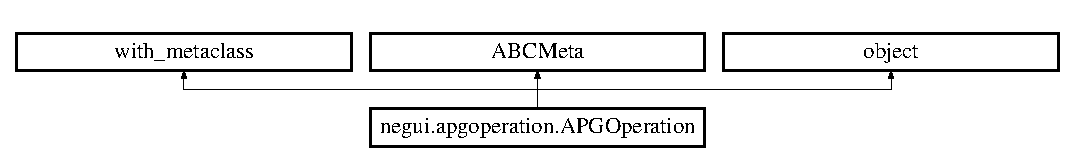
\includegraphics[height=2.000000cm]{classnegui_1_1apgoperation_1_1APGOperation}
\end{center}
\end{figure}
\subsection*{Public Member Functions}
\begin{DoxyCompactItemize}
\item 
def {\bfseries \+\_\+\+\_\+init\+\_\+\+\_\+} (self, o\+\_\+input, o\+\_\+output)\hypertarget{classnegui_1_1apgoperation_1_1APGOperation_a4c8ae262ea950770883a02d8f062bfc1}{}\label{classnegui_1_1apgoperation_1_1APGOperation_a4c8ae262ea950770883a02d8f062bfc1}

\item 
def {\bfseries prepare\+Op} (self)\hypertarget{classnegui_1_1apgoperation_1_1APGOperation_a3167f1a64c3473f000a6268ff6d40955}{}\label{classnegui_1_1apgoperation_1_1APGOperation_a3167f1a64c3473f000a6268ff6d40955}

\item 
def {\bfseries do\+Op} (self)\hypertarget{classnegui_1_1apgoperation_1_1APGOperation_a087b1072a7deae2b98e2c085f0ebebbe}{}\label{classnegui_1_1apgoperation_1_1APGOperation_a087b1072a7deae2b98e2c085f0ebebbe}

\item 
def {\bfseries deliver\+Results} (self)\hypertarget{classnegui_1_1apgoperation_1_1APGOperation_a10f5ecf8d47ef55ba78a8a7a45ad1a6b}{}\label{classnegui_1_1apgoperation_1_1APGOperation_a10f5ecf8d47ef55ba78a8a7a45ad1a6b}

\item 
def {\bfseries input} (self)\hypertarget{classnegui_1_1apgoperation_1_1APGOperation_a7c10319113f046132fe6049896bcd485}{}\label{classnegui_1_1apgoperation_1_1APGOperation_a7c10319113f046132fe6049896bcd485}

\item 
def {\bfseries input} (self, o\+\_\+input\+\_\+object)\hypertarget{classnegui_1_1apgoperation_1_1APGOperation_a44b8970179dccb0e54c3a35463aa5c72}{}\label{classnegui_1_1apgoperation_1_1APGOperation_a44b8970179dccb0e54c3a35463aa5c72}

\item 
def {\bfseries input} (self)\hypertarget{classnegui_1_1apgoperation_1_1APGOperation_a7c10319113f046132fe6049896bcd485}{}\label{classnegui_1_1apgoperation_1_1APGOperation_a7c10319113f046132fe6049896bcd485}

\item 
def {\bfseries output} (self)\hypertarget{classnegui_1_1apgoperation_1_1APGOperation_a70a4663961a30ab0405701072c78f759}{}\label{classnegui_1_1apgoperation_1_1APGOperation_a70a4663961a30ab0405701072c78f759}

\item 
def {\bfseries output} (self, o\+\_\+output\+\_\+object)\hypertarget{classnegui_1_1apgoperation_1_1APGOperation_a92751ec3a6053de0e8638df3d1b122ff}{}\label{classnegui_1_1apgoperation_1_1APGOperation_a92751ec3a6053de0e8638df3d1b122ff}

\item 
def {\bfseries output} (self)\hypertarget{classnegui_1_1apgoperation_1_1APGOperation_a70a4663961a30ab0405701072c78f759}{}\label{classnegui_1_1apgoperation_1_1APGOperation_a70a4663961a30ab0405701072c78f759}

\end{DoxyCompactItemize}


\subsection{Detailed Description}
\begin{DoxyVerb}Abstract class PGOperation is to be implemented by subclasses.
Wraps the code required to perform a pop gen analysis, such as a simuPop simulation,
Or an Ne calculation.  Instantiated subclass objects are the expected type members 
of the PGGuiApp class objects attribute "gp_operation".
\end{DoxyVerb}
 

Definition at line 15 of file apgoperation.\+py.



The documentation for this class was generated from the following file\+:\begin{DoxyCompactItemize}
\item 
apgoperation.\+py\end{DoxyCompactItemize}

\hypertarget{classnegui_1_1createtooltip_1_1CreateToolTip}{}\section{negui.\+createtooltip.\+Create\+Tool\+Tip Class Reference}
\label{classnegui_1_1createtooltip_1_1CreateToolTip}\index{negui.\+createtooltip.\+Create\+Tool\+Tip@{negui.\+createtooltip.\+Create\+Tool\+Tip}}
Inheritance diagram for negui.\+createtooltip.\+Create\+Tool\+Tip\+:\begin{figure}[H]
\begin{center}
\leavevmode
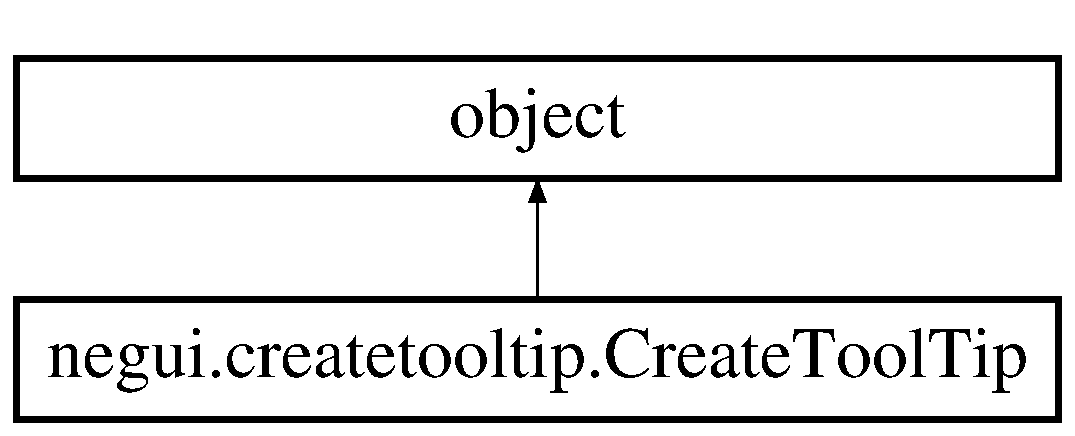
\includegraphics[height=2.000000cm]{classnegui_1_1createtooltip_1_1CreateToolTip}
\end{center}
\end{figure}
\subsection*{Public Member Functions}
\begin{DoxyCompactItemize}
\item 
def \hyperlink{classnegui_1_1createtooltip_1_1CreateToolTip_aec360f7f4bfc95876b04ad68a7c54140}{\+\_\+\+\_\+init\+\_\+\+\_\+} (self, widget, text=\textquotesingle{}widget info\textquotesingle{}, i\+\_\+font\+\_\+size=10)
\item 
def \hyperlink{classnegui_1_1createtooltip_1_1CreateToolTip_ab37624e73833e8ba485d10410c5986bb}{enter} (self, event=None)
\item 
def \hyperlink{classnegui_1_1createtooltip_1_1CreateToolTip_aa6f6887d11b3e07e5f6e12b267412fae}{close} (self, event=None)
\end{DoxyCompactItemize}
\subsection*{Public Attributes}
\begin{DoxyCompactItemize}
\item 
{\bfseries tw}\hypertarget{classnegui_1_1createtooltip_1_1CreateToolTip_ac47a0f82a5a354f6c8914c4631d1a0cf}{}\label{classnegui_1_1createtooltip_1_1CreateToolTip_ac47a0f82a5a354f6c8914c4631d1a0cf}

\item 
{\bfseries widget}\hypertarget{classnegui_1_1createtooltip_1_1CreateToolTip_a6619448e568b135261fd02a6d9b36725}{}\label{classnegui_1_1createtooltip_1_1CreateToolTip_a6619448e568b135261fd02a6d9b36725}

\item 
{\bfseries text}\hypertarget{classnegui_1_1createtooltip_1_1CreateToolTip_a198b3395803def62ec55ed820e756b11}{}\label{classnegui_1_1createtooltip_1_1CreateToolTip_a198b3395803def62ec55ed820e756b11}

\item 
{\bfseries font\+\_\+size}\hypertarget{classnegui_1_1createtooltip_1_1CreateToolTip_a42f2306cb6ad9995d76e0eb556416bed}{}\label{classnegui_1_1createtooltip_1_1CreateToolTip_a42f2306cb6ad9995d76e0eb556416bed}

\end{DoxyCompactItemize}


\subsection{Detailed Description}
\begin{DoxyVerb}Creates a tooltip for a given widget.
This code was copied from 
https://www.daniweb.com/programming/software-development/code/484591/a-tooltip-class-for-tkinter
tk_ToolTip_class101.py
gives a Tkinter widget a tooltip as the mouse is above the widget
tested with Python27 and Python34  by  vegaseat  09sep2014\end{DoxyVerb}
 

Definition at line 38 of file createtooltip.\+py.



\subsection{Constructor \& Destructor Documentation}
\index{negui\+::createtooltip\+::\+Create\+Tool\+Tip@{negui\+::createtooltip\+::\+Create\+Tool\+Tip}!\+\_\+\+\_\+init\+\_\+\+\_\+@{\+\_\+\+\_\+init\+\_\+\+\_\+}}
\index{\+\_\+\+\_\+init\+\_\+\+\_\+@{\+\_\+\+\_\+init\+\_\+\+\_\+}!negui\+::createtooltip\+::\+Create\+Tool\+Tip@{negui\+::createtooltip\+::\+Create\+Tool\+Tip}}
\subsubsection[{\texorpdfstring{\+\_\+\+\_\+init\+\_\+\+\_\+(self, widget, text=\textquotesingle{}widget info\textquotesingle{}, i\+\_\+font\+\_\+size=10)}{__init__(self, widget, text='widget info', i_font_size=10)}}]{\setlength{\rightskip}{0pt plus 5cm}def negui.\+createtooltip.\+Create\+Tool\+Tip.\+\_\+\+\_\+init\+\_\+\+\_\+ (
\begin{DoxyParamCaption}
\item[{}]{self, }
\item[{}]{widget, }
\item[{}]{text = {\ttfamily \textquotesingle{}widget~info\textquotesingle{}}, }
\item[{}]{i\+\_\+font\+\_\+size = {\ttfamily 10}}
\end{DoxyParamCaption}
)}\hypertarget{classnegui_1_1createtooltip_1_1CreateToolTip_aec360f7f4bfc95876b04ad68a7c54140}{}\label{classnegui_1_1createtooltip_1_1CreateToolTip_aec360f7f4bfc95876b04ad68a7c54140}
\begin{DoxyVerb}Ted added, in case close gets called before enter,
we'll have tw inditialzed to None.
\end{DoxyVerb}
 

Definition at line 48 of file createtooltip.\+py.


\begin{DoxyCode}
48     \textcolor{keyword}{def }\hyperlink{classnegui_1_1createtooltip_1_1CreateToolTip_aec360f7f4bfc95876b04ad68a7c54140}{\_\_init\_\_}(self, widget, text='widget info', i\_font\_size=10 ):
49         \textcolor{stringliteral}{'''}
50 \textcolor{stringliteral}{        Ted added, in case close gets called before enter,}
51 \textcolor{stringliteral}{        we'll have tw inditialzed to None.}
52 \textcolor{stringliteral}{        '''}
53         self.\hyperlink{classnegui_1_1createtooltip_1_1CreateToolTip_ac47a0f82a5a354f6c8914c4631d1a0cf}{tw}=\textcolor{keywordtype}{None}
54         self.\hyperlink{classnegui_1_1createtooltip_1_1CreateToolTip_a6619448e568b135261fd02a6d9b36725}{widget} = widget
55         self.\hyperlink{classnegui_1_1createtooltip_1_1CreateToolTip_a198b3395803def62ec55ed820e756b11}{text} = text
56         self.widget.bind(\textcolor{stringliteral}{"<Enter>"}, self.\hyperlink{classnegui_1_1createtooltip_1_1CreateToolTip_ab37624e73833e8ba485d10410c5986bb}{enter})
57         self.widget.bind(\textcolor{stringliteral}{"<Leave>"}, self.\hyperlink{classnegui_1_1createtooltip_1_1CreateToolTip_aa6f6887d11b3e07e5f6e12b267412fae}{close})
58         \textcolor{stringliteral}{'''}
59 \textcolor{stringliteral}{        Trying to fix bug in which tooltop persists}
60 \textcolor{stringliteral}{        permanently.}
61 \textcolor{stringliteral}{        '''}
62         self.widget.bind( \textcolor{stringliteral}{"<FocusOut>"}, self.\hyperlink{classnegui_1_1createtooltip_1_1CreateToolTip_aa6f6887d11b3e07e5f6e12b267412fae}{close})
63         self.\hyperlink{classnegui_1_1createtooltip_1_1CreateToolTip_a42f2306cb6ad9995d76e0eb556416bed}{font\_size}=i\_font\_size
\end{DoxyCode}


\subsection{Member Function Documentation}
\index{negui\+::createtooltip\+::\+Create\+Tool\+Tip@{negui\+::createtooltip\+::\+Create\+Tool\+Tip}!close@{close}}
\index{close@{close}!negui\+::createtooltip\+::\+Create\+Tool\+Tip@{negui\+::createtooltip\+::\+Create\+Tool\+Tip}}
\subsubsection[{\texorpdfstring{close(self, event=\+None)}{close(self, event=None)}}]{\setlength{\rightskip}{0pt plus 5cm}def negui.\+createtooltip.\+Create\+Tool\+Tip.\+close (
\begin{DoxyParamCaption}
\item[{}]{self, }
\item[{}]{event = {\ttfamily None}}
\end{DoxyParamCaption}
)}\hypertarget{classnegui_1_1createtooltip_1_1CreateToolTip_aa6f6887d11b3e07e5f6e12b267412fae}{}\label{classnegui_1_1createtooltip_1_1CreateToolTip_aa6f6887d11b3e07e5f6e12b267412fae}
\begin{DoxyVerb}Code testing and assigning tw for/to None,
added 2016_10_31 to more consistently manage 
the tw member.  See the def "enter",
for more details on some buggy
behavior.
\end{DoxyVerb}
 

Definition at line 110 of file createtooltip.\+py.


\begin{DoxyCode}
110     \textcolor{keyword}{def }\hyperlink{classnegui_1_1createtooltip_1_1CreateToolTip_aa6f6887d11b3e07e5f6e12b267412fae}{close}(self, event=None):
111         \textcolor{stringliteral}{'''}
112 \textcolor{stringliteral}{        Code testing and assigning tw for/to None,}
113 \textcolor{stringliteral}{        added 2016\_10\_31 to more consistently manage }
114 \textcolor{stringliteral}{        the tw member.  See the def "enter",}
115 \textcolor{stringliteral}{        for more details on some buggy}
116 \textcolor{stringliteral}{        behavior.}
117 \textcolor{stringliteral}{        '''}
118         \textcolor{keywordflow}{if} self.\hyperlink{classnegui_1_1createtooltip_1_1CreateToolTip_ac47a0f82a5a354f6c8914c4631d1a0cf}{tw} \textcolor{keywordflow}{is} \textcolor{keywordflow}{not} \textcolor{keywordtype}{None}:
119             self.tw.destroy()
120         \textcolor{comment}{#end if}
121 
122         \textcolor{stringliteral}{'''}
123 \textcolor{stringliteral}{        Consistent value for tw after call}
124 \textcolor{stringliteral}{        to close, no matter its previous one:}
125 \textcolor{stringliteral}{        '''}
126         self.\hyperlink{classnegui_1_1createtooltip_1_1CreateToolTip_ac47a0f82a5a354f6c8914c4631d1a0cf}{tw} = \textcolor{keywordtype}{None}
\end{DoxyCode}
\index{negui\+::createtooltip\+::\+Create\+Tool\+Tip@{negui\+::createtooltip\+::\+Create\+Tool\+Tip}!enter@{enter}}
\index{enter@{enter}!negui\+::createtooltip\+::\+Create\+Tool\+Tip@{negui\+::createtooltip\+::\+Create\+Tool\+Tip}}
\subsubsection[{\texorpdfstring{enter(self, event=\+None)}{enter(self, event=None)}}]{\setlength{\rightskip}{0pt plus 5cm}def negui.\+createtooltip.\+Create\+Tool\+Tip.\+enter (
\begin{DoxyParamCaption}
\item[{}]{self, }
\item[{}]{event = {\ttfamily None}}
\end{DoxyParamCaption}
)}\hypertarget{classnegui_1_1createtooltip_1_1CreateToolTip_ab37624e73833e8ba485d10410c5986bb}{}\label{classnegui_1_1createtooltip_1_1CreateToolTip_ab37624e73833e8ba485d10410c5986bb}
\begin{DoxyVerb}Code added 2016_10_31, setting the tw member 
to None in __init__ (see above), then always 
testing it before recreating it, seems to have
resolved a bug, seemingly only associated with
comboboxes and very rarely with text boxes,
via my KeyVal objects, in which the tooltip
window was created but never closed.  This
was reliably invoked by using the keyboard
to update a combobox, while the mouse was still
over the control. On th ekeyboard selection, the
tooltip windows would appear and persist, while
new ones would appear over it.  This management
and testing of the tw member seems to have solved
it.
\end{DoxyVerb}
 

Definition at line 66 of file createtooltip.\+py.


\begin{DoxyCode}
66     \textcolor{keyword}{def }\hyperlink{classnegui_1_1createtooltip_1_1CreateToolTip_ab37624e73833e8ba485d10410c5986bb}{enter}(self, event=None):
67 
68         \textcolor{stringliteral}{'''}
69 \textcolor{stringliteral}{        Code added 2016\_10\_31, setting the tw member }
70 \textcolor{stringliteral}{        to None in \_\_init\_\_ (see above), then always }
71 \textcolor{stringliteral}{        testing it before recreating it, seems to have}
72 \textcolor{stringliteral}{        resolved a bug, seemingly only associated with}
73 \textcolor{stringliteral}{        comboboxes and very rarely with text boxes,}
74 \textcolor{stringliteral}{        via my KeyVal objects, in which the tooltip}
75 \textcolor{stringliteral}{        window was created but never closed.  This}
76 \textcolor{stringliteral}{        was reliably invoked by using the keyboard}
77 \textcolor{stringliteral}{        to update a combobox, while the mouse was still}
78 \textcolor{stringliteral}{        over the control. On th ekeyboard selection, the}
79 \textcolor{stringliteral}{        tooltip windows would appear and persist, while}
80 \textcolor{stringliteral}{        new ones would appear over it.  This management}
81 \textcolor{stringliteral}{        and testing of the tw member seems to have solved}
82 \textcolor{stringliteral}{        it.}
83 \textcolor{stringliteral}{        '''}
84         \textcolor{keywordflow}{if} self.\hyperlink{classnegui_1_1createtooltip_1_1CreateToolTip_ac47a0f82a5a354f6c8914c4631d1a0cf}{tw} \textcolor{keywordflow}{is} \textcolor{keywordtype}{None}:
85             \textcolor{stringliteral}{'''}
86 \textcolor{stringliteral}{            I added 2016\_10\_31}
87 \textcolor{stringliteral}{            constants used below,}
88 \textcolor{stringliteral}{            instead of literals,}
89 \textcolor{stringliteral}{            '''} 
90             PADX=25
91             PADY=20
92 
93             x = y = 0
94             x, y, cx, cy = self.widget.bbox(\textcolor{stringliteral}{"insert"})
95             x += self.widget.winfo\_rootx() + PADX
96             y += self.widget.winfo\_rooty() + PADY
97             \textcolor{comment}{# creates a toplevel window}
98             self.\hyperlink{classnegui_1_1createtooltip_1_1CreateToolTip_ac47a0f82a5a354f6c8914c4631d1a0cf}{tw} = tk.Toplevel(self.\hyperlink{classnegui_1_1createtooltip_1_1CreateToolTip_a6619448e568b135261fd02a6d9b36725}{widget})
99             \textcolor{comment}{# Leaves only the label and removes the app window}
100             self.tw.wm\_overrideredirect(\textcolor{keyword}{True})
101             self.tw.wm\_geometry(\textcolor{stringliteral}{"+%d+%d"} % (x, y))
102             label = tk.Label(self.\hyperlink{classnegui_1_1createtooltip_1_1CreateToolTip_ac47a0f82a5a354f6c8914c4631d1a0cf}{tw}, text=self.\hyperlink{classnegui_1_1createtooltip_1_1CreateToolTip_a198b3395803def62ec55ed820e756b11}{text}, justify=\textcolor{stringliteral}{'left'},
103                            background=\textcolor{stringliteral}{'yellow'}, relief=\textcolor{stringliteral}{'solid'}, borderwidth=1,
104                            font=(\textcolor{stringliteral}{"times"}, self.\hyperlink{classnegui_1_1createtooltip_1_1CreateToolTip_a42f2306cb6ad9995d76e0eb556416bed}{font\_size}, \textcolor{stringliteral}{"normal"}))
105             label.pack(ipadx=1)
106         \textcolor{comment}{#end if self.tw is  None}
107 
\end{DoxyCode}


The documentation for this class was generated from the following file\+:\begin{DoxyCompactItemize}
\item 
createtooltip.\+py\end{DoxyCompactItemize}

\hypertarget{classnegui_1_1pgdriveneestimator_1_1DebugMode}{}\section{negui.\+pgdriveneestimator.\+Debug\+Mode Class Reference}
\label{classnegui_1_1pgdriveneestimator_1_1DebugMode}\index{negui.\+pgdriveneestimator.\+Debug\+Mode@{negui.\+pgdriveneestimator.\+Debug\+Mode}}
Inheritance diagram for negui.\+pgdriveneestimator.\+Debug\+Mode\+:\begin{figure}[H]
\begin{center}
\leavevmode
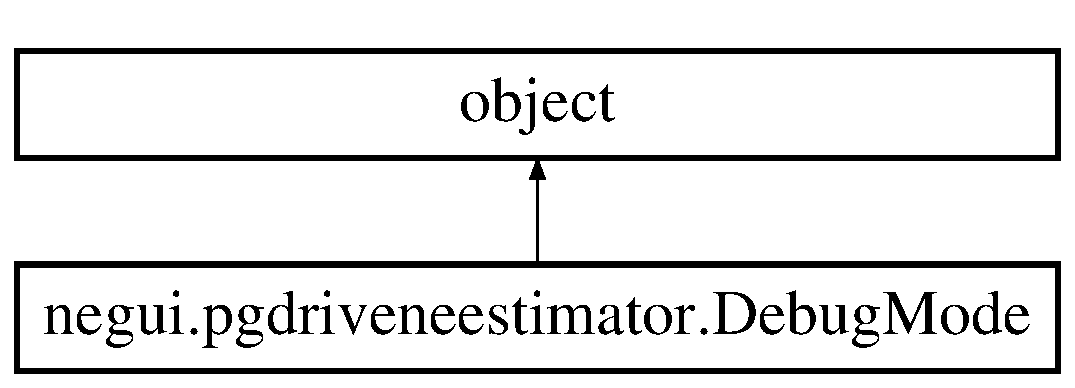
\includegraphics[height=2.000000cm]{classnegui_1_1pgdriveneestimator_1_1DebugMode}
\end{center}
\end{figure}
\subsection*{Public Member Functions}
\begin{DoxyCompactItemize}
\item 
def {\bfseries \+\_\+\+\_\+init\+\_\+\+\_\+} (self, s\+\_\+mode=\char`\"{}no\+\_\+debug\char`\"{})\hypertarget{classnegui_1_1pgdriveneestimator_1_1DebugMode_ad28ea39a3d3a4163f408348fbcdf8207}{}\label{classnegui_1_1pgdriveneestimator_1_1DebugMode_ad28ea39a3d3a4163f408348fbcdf8207}

\item 
def {\bfseries is\+Set} (self, i\+\_\+flag)\hypertarget{classnegui_1_1pgdriveneestimator_1_1DebugMode_ab345367b1debb52518dd753b4c740d3c}{}\label{classnegui_1_1pgdriveneestimator_1_1DebugMode_ab345367b1debb52518dd753b4c740d3c}

\item 
def {\bfseries mode} (self)\hypertarget{classnegui_1_1pgdriveneestimator_1_1DebugMode_a877126bd7e0e8a571b90e0be7436568b}{}\label{classnegui_1_1pgdriveneestimator_1_1DebugMode_a877126bd7e0e8a571b90e0be7436568b}

\item 
def {\bfseries mode} (self, s\+\_\+mode)\hypertarget{classnegui_1_1pgdriveneestimator_1_1DebugMode_ae3f4deed085cffa67a10aa94f857ade0}{}\label{classnegui_1_1pgdriveneestimator_1_1DebugMode_ae3f4deed085cffa67a10aa94f857ade0}

\end{DoxyCompactItemize}
\subsection*{Static Public Attributes}
\begin{DoxyCompactItemize}
\item 
list {\bfseries M\+O\+D\+ES} = \mbox{[} \char`\"{}no\+\_\+debug\char`\"{}, \char`\"{}debug1\char`\"{}, \char`\"{}debug2\char`\"{}, \char`\"{}debug3\char`\"{}, \char`\"{}testserial\char`\"{}, \char`\"{}testmulti\char`\"{} \mbox{]}\hypertarget{classnegui_1_1pgdriveneestimator_1_1DebugMode_a7f3d898bacc395557b8cb40337cfa7e6}{}\label{classnegui_1_1pgdriveneestimator_1_1DebugMode_a7f3d898bacc395557b8cb40337cfa7e6}

\item 
string {\bfseries N\+O\+\_\+\+D\+E\+B\+UG} = \char`\"{}no\+\_\+debug\char`\"{}\hypertarget{classnegui_1_1pgdriveneestimator_1_1DebugMode_a68f03775793d9894bdb28c34f9b33a0c}{}\label{classnegui_1_1pgdriveneestimator_1_1DebugMode_a68f03775793d9894bdb28c34f9b33a0c}

\item 
string {\bfseries M\+A\+K\+E\+\_\+\+T\+A\+B\+LE} = \char`\"{}debug1\char`\"{}\hypertarget{classnegui_1_1pgdriveneestimator_1_1DebugMode_ad287b36021099229f7f4fc86ebc5774e}{}\label{classnegui_1_1pgdriveneestimator_1_1DebugMode_ad287b36021099229f7f4fc86ebc5774e}

\item 
string {\bfseries M\+A\+K\+E\+\_\+\+T\+A\+B\+L\+E\+\_\+\+A\+N\+D\+\_\+\+K\+E\+E\+P\+\_\+\+F\+I\+L\+ES} = \char`\"{}debug2\char`\"{}\hypertarget{classnegui_1_1pgdriveneestimator_1_1DebugMode_a9fb4c700600776a72a359483a08928ea}{}\label{classnegui_1_1pgdriveneestimator_1_1DebugMode_a9fb4c700600776a72a359483a08928ea}

\item 
string {\bfseries A\+L\+L\+\_\+\+D\+E\+B\+U\+G\+\_\+\+O\+P\+T\+I\+O\+NS} = \char`\"{}debug3\char`\"{}\hypertarget{classnegui_1_1pgdriveneestimator_1_1DebugMode_a9f3faea66935c3978c447de9baf0f144}{}\label{classnegui_1_1pgdriveneestimator_1_1DebugMode_a9f3faea66935c3978c447de9baf0f144}

\item 
string {\bfseries T\+E\+S\+T\+\_\+\+S\+E\+R\+I\+AL} = \char`\"{}testserial\char`\"{}\hypertarget{classnegui_1_1pgdriveneestimator_1_1DebugMode_aec7b522f17d7790b980ae128a4445b0e}{}\label{classnegui_1_1pgdriveneestimator_1_1DebugMode_aec7b522f17d7790b980ae128a4445b0e}

\item 
string {\bfseries T\+E\+S\+T\+\_\+\+M\+U\+L\+TI} = \char`\"{}testmulti\char`\"{}\hypertarget{classnegui_1_1pgdriveneestimator_1_1DebugMode_a8a5f8c6fe20337dd6b894aba21bd1e17}{}\label{classnegui_1_1pgdriveneestimator_1_1DebugMode_a8a5f8c6fe20337dd6b894aba21bd1e17}

\item 
int {\bfseries K\+E\+E\+P\+\_\+\+R\+E\+P\+L\+I\+C\+A\+T\+E\+\_\+\+G\+E\+N\+E\+P\+O\+P\+\_\+\+F\+I\+L\+ES} = 1\hypertarget{classnegui_1_1pgdriveneestimator_1_1DebugMode_a28d1c7693a4bec8f391bef360d51b463}{}\label{classnegui_1_1pgdriveneestimator_1_1DebugMode_a28d1c7693a4bec8f391bef360d51b463}

\item 
int {\bfseries K\+E\+E\+P\+\_\+\+E\+S\+T\+I\+M\+A\+T\+O\+R\+\_\+\+F\+I\+L\+ES} = 2\hypertarget{classnegui_1_1pgdriveneestimator_1_1DebugMode_a2f02d51f5d3a4a6c9cfaa8d0f6ea1879}{}\label{classnegui_1_1pgdriveneestimator_1_1DebugMode_a2f02d51f5d3a4a6c9cfaa8d0f6ea1879}

\item 
int {\bfseries M\+A\+K\+E\+\_\+\+I\+N\+D\+I\+V\+\_\+\+T\+A\+B\+LE} = 4\hypertarget{classnegui_1_1pgdriveneestimator_1_1DebugMode_a1f5d7e71208d6a4a9d7a63b0207e1ab8}{}\label{classnegui_1_1pgdriveneestimator_1_1DebugMode_a1f5d7e71208d6a4a9d7a63b0207e1ab8}

\item 
int {\bfseries A\+L\+L\+O\+W\+\_\+\+M\+U\+L\+T\+I\+\_\+\+P\+R\+O\+C\+E\+S\+S\+ES} = 8\hypertarget{classnegui_1_1pgdriveneestimator_1_1DebugMode_af0b037fef1711a912d1f83ed61f57097}{}\label{classnegui_1_1pgdriveneestimator_1_1DebugMode_af0b037fef1711a912d1f83ed61f57097}

\item 
int {\bfseries P\+R\+I\+N\+T\+\_\+\+R\+E\+P\+L\+I\+C\+A\+T\+E\+\_\+\+S\+E\+L\+E\+C\+T\+I\+O\+NS} = 16\hypertarget{classnegui_1_1pgdriveneestimator_1_1DebugMode_a238432e744ac313e2ce4d7de801ffe92}{}\label{classnegui_1_1pgdriveneestimator_1_1DebugMode_a238432e744ac313e2ce4d7de801ffe92}

\item 
int {\bfseries K\+E\+E\+P\+\_\+\+N\+O\+D\+A\+T\+\_\+\+F\+I\+L\+ES} = 32\hypertarget{classnegui_1_1pgdriveneestimator_1_1DebugMode_ac55e866ab4d12b084f2480d625c9dbb8}{}\label{classnegui_1_1pgdriveneestimator_1_1DebugMode_ac55e866ab4d12b084f2480d625c9dbb8}

\item 
int {\bfseries K\+E\+E\+P\+\_\+\+N\+E\+X\+T\+P\+\_\+\+F\+I\+L\+ES} = 64\hypertarget{classnegui_1_1pgdriveneestimator_1_1DebugMode_a13096a90911741639b1eea0e1595cb2b}{}\label{classnegui_1_1pgdriveneestimator_1_1DebugMode_a13096a90911741639b1eea0e1595cb2b}

\end{DoxyCompactItemize}


\subsection{Detailed Description}


Definition at line 273 of file pgdriveneestimator.\+py.



The documentation for this class was generated from the following file\+:\begin{DoxyCompactItemize}
\item 
pgdriveneestimator.\+py\end{DoxyCompactItemize}

\hypertarget{classnegui_1_1pgguiutilities_1_1FrameContainerScrolled}{}\section{negui.\+pgguiutilities.\+Frame\+Container\+Scrolled Class Reference}
\label{classnegui_1_1pgguiutilities_1_1FrameContainerScrolled}\index{negui.\+pgguiutilities.\+Frame\+Container\+Scrolled@{negui.\+pgguiutilities.\+Frame\+Container\+Scrolled}}
Inheritance diagram for negui.\+pgguiutilities.\+Frame\+Container\+Scrolled\+:\begin{figure}[H]
\begin{center}
\leavevmode
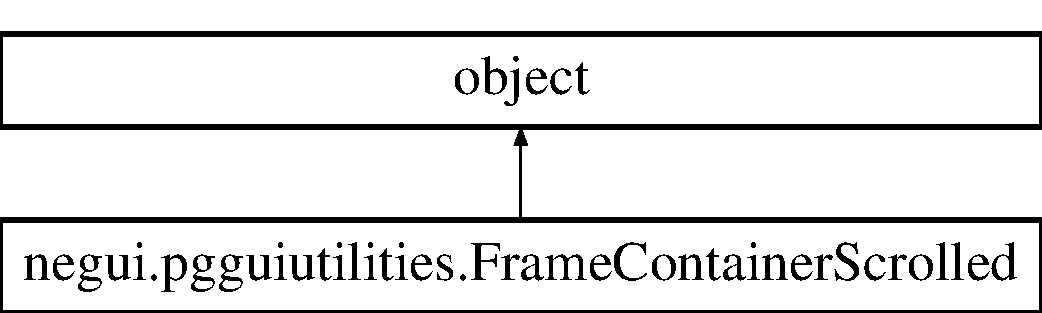
\includegraphics[height=2.000000cm]{classnegui_1_1pgguiutilities_1_1FrameContainerScrolled}
\end{center}
\end{figure}
\subsection*{Public Member Functions}
\begin{DoxyCompactItemize}
\item 
def {\bfseries \+\_\+\+\_\+init\+\_\+\+\_\+} (self, o\+\_\+parent\+\_\+frame, o\+\_\+child\+\_\+frame, o\+\_\+canvas, i\+\_\+scroll\+\_\+direction=S\+C\+R\+O\+L\+L\+V\+E\+R\+T\+I\+C\+AL)\hypertarget{classnegui_1_1pgguiutilities_1_1FrameContainerScrolled_a6e6e85912ffe9db1e258483327c8c7bb}{}\label{classnegui_1_1pgguiutilities_1_1FrameContainerScrolled_a6e6e85912ffe9db1e258483327c8c7bb}

\end{DoxyCompactItemize}
\subsection*{Static Public Attributes}
\begin{DoxyCompactItemize}
\item 
int {\bfseries S\+C\+R\+O\+L\+L\+V\+E\+R\+T\+I\+C\+AL} = 0\hypertarget{classnegui_1_1pgguiutilities_1_1FrameContainerScrolled_ab9206d87d03f06b9ebfc7e93460aba30}{}\label{classnegui_1_1pgguiutilities_1_1FrameContainerScrolled_ab9206d87d03f06b9ebfc7e93460aba30}

\item 
int {\bfseries S\+C\+R\+O\+L\+L\+H\+O\+R\+I\+Z\+O\+N\+T\+AL} = 1\hypertarget{classnegui_1_1pgguiutilities_1_1FrameContainerScrolled_af674b82923a9232afeba8f2512727bbf}{}\label{classnegui_1_1pgguiutilities_1_1FrameContainerScrolled_af674b82923a9232afeba8f2512727bbf}

\end{DoxyCompactItemize}


\subsection{Detailed Description}
\begin{DoxyVerb}Description
Objects are arrangements of two Frames and a 
Canvas, such that one frame contains the 
canvas and 2nd frame, and the 2nd frame 
is scrollable, either vertically or horizontally 
(but not yet both, as of Thu Jun  2 19:59:32 MDT 2016 )


Note that this is not a Tkinter object, but
simply accomplishes the arragnement. 

Note that this uses Fred Lundh's AutoScrollbar class
(from http://effbot.org/zone/tkinter-autoscrollbar.htm)
and depends on using only the grid geometry manager to place
the scrollbar.
\end{DoxyVerb}
 

Definition at line 1155 of file pgguiutilities.\+py.



The documentation for this class was generated from the following file\+:\begin{DoxyCompactItemize}
\item 
pgguiutilities.\+py\end{DoxyCompactItemize}

\hypertarget{classnegui_1_1pgguiutilities_1_1FrameContainerVScroll}{}\section{negui.\+pgguiutilities.\+Frame\+Container\+V\+Scroll Class Reference}
\label{classnegui_1_1pgguiutilities_1_1FrameContainerVScroll}\index{negui.\+pgguiutilities.\+Frame\+Container\+V\+Scroll@{negui.\+pgguiutilities.\+Frame\+Container\+V\+Scroll}}
Inheritance diagram for negui.\+pgguiutilities.\+Frame\+Container\+V\+Scroll\+:\begin{figure}[H]
\begin{center}
\leavevmode
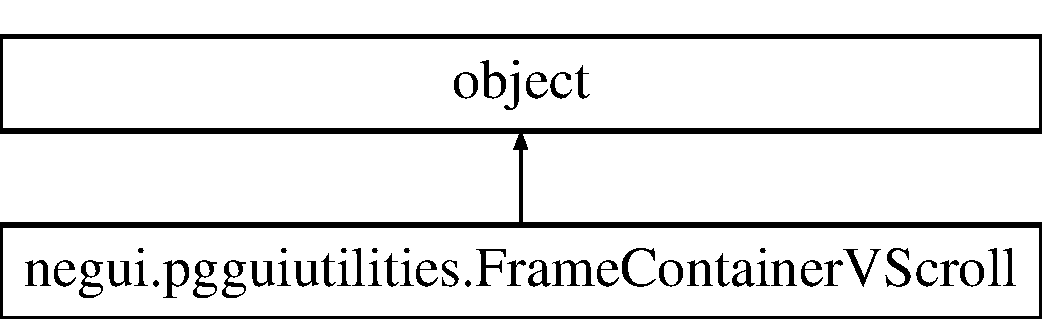
\includegraphics[height=2.000000cm]{classnegui_1_1pgguiutilities_1_1FrameContainerVScroll}
\end{center}
\end{figure}
\subsection*{Public Member Functions}
\begin{DoxyCompactItemize}
\item 
def {\bfseries \+\_\+\+\_\+init\+\_\+\+\_\+} (self, o\+\_\+parent\+\_\+frame, o\+\_\+child\+\_\+frame, o\+\_\+canvas)\hypertarget{classnegui_1_1pgguiutilities_1_1FrameContainerVScroll_a77671bf20cb4175f0788de78bda3445f}{}\label{classnegui_1_1pgguiutilities_1_1FrameContainerVScroll_a77671bf20cb4175f0788de78bda3445f}

\end{DoxyCompactItemize}


\subsection{Detailed Description}
\begin{DoxyVerb}Description
Objects are arrangements of two Frames and a 
Canvas, such that one frame contains the 
canvas and 2nd frame, and the 2nd frame 
is vertically scrollable.

Note that this is not a Tkinter object, but
simply accomplishes the arragnement. 

Note that this uses Fred Lundh's AutoScrollbar class
(from http://effbot.org/zone/tkinter-autoscrollbar.htm)
and depends on using only the grid geometry manager to place
the scrollbar.
\end{DoxyVerb}
 

Definition at line 1277 of file pgguiutilities.\+py.



The documentation for this class was generated from the following file\+:\begin{DoxyCompactItemize}
\item 
pgguiutilities.\+py\end{DoxyCompactItemize}

\hypertarget{classnegui_1_1genepopfilemanager_1_1GenepopFileManager}{}\section{negui.\+genepopfilemanager.\+Genepop\+File\+Manager Class Reference}
\label{classnegui_1_1genepopfilemanager_1_1GenepopFileManager}\index{negui.\+genepopfilemanager.\+Genepop\+File\+Manager@{negui.\+genepopfilemanager.\+Genepop\+File\+Manager}}
Inheritance diagram for negui.\+genepopfilemanager.\+Genepop\+File\+Manager\+:\begin{figure}[H]
\begin{center}
\leavevmode
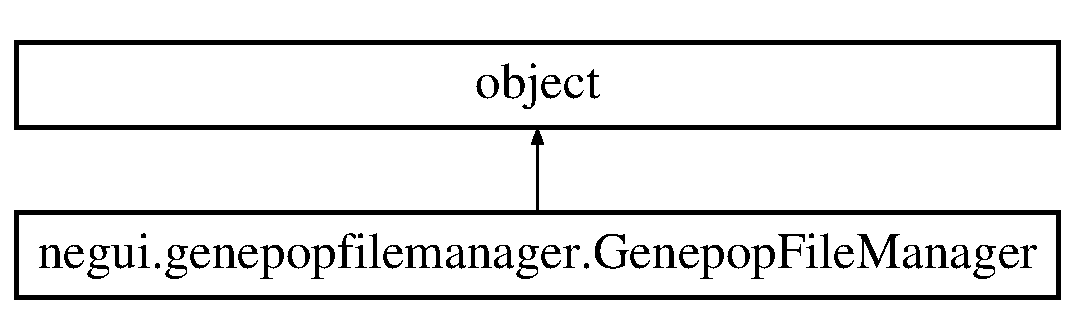
\includegraphics[height=2.000000cm]{classnegui_1_1genepopfilemanager_1_1GenepopFileManager}
\end{center}
\end{figure}
\subsection*{Public Member Functions}
\begin{DoxyCompactItemize}
\item 
def {\bfseries \+\_\+\+\_\+init\+\_\+\+\_\+} (self, s\+\_\+filename)\hypertarget{classnegui_1_1genepopfilemanager_1_1GenepopFileManager_a8563b3299666d02d45c9acd64f450c51}{}\label{classnegui_1_1genepopfilemanager_1_1GenepopFileManager_a8563b3299666d02d45c9acd64f450c51}

\item 
def {\bfseries write\+Gene\+Pop\+File} (self, s\+\_\+newfilename, s\+\_\+pop\+\_\+subsample\+\_\+tag=None, s\+\_\+indiv\+\_\+subsample\+\_\+tag=None, s\+\_\+loci\+\_\+subsample\+\_\+tag=None, i\+\_\+min\+\_\+pop\+\_\+size=0)\hypertarget{classnegui_1_1genepopfilemanager_1_1GenepopFileManager_a7390cad5840454284e816679a87d84df}{}\label{classnegui_1_1genepopfilemanager_1_1GenepopFileManager_a7390cad5840454284e816679a87d84df}

\item 
def {\bfseries print\+Gene\+Pop\+File} (self, s\+\_\+pop\+\_\+subsample\+\_\+tag=None, s\+\_\+indiv\+\_\+subsample\+\_\+tag=None, s\+\_\+loci\+\_\+subsample\+\_\+tag=None, i\+\_\+min\+\_\+pop\+\_\+size=0)\hypertarget{classnegui_1_1genepopfilemanager_1_1GenepopFileManager_a35aa30c43ab4a5e7762bf8c722314727}{}\label{classnegui_1_1genepopfilemanager_1_1GenepopFileManager_a35aa30c43ab4a5e7762bf8c722314727}

\item 
def {\bfseries get\+List\+Individual\+Numbers} (self, i\+\_\+pop\+\_\+number=1, s\+\_\+indiv\+\_\+subsample\+\_\+tag=None)\hypertarget{classnegui_1_1genepopfilemanager_1_1GenepopFileManager_a652029f0a6e0668e0b75c9683dae0ffd}{}\label{classnegui_1_1genepopfilemanager_1_1GenepopFileManager_a652029f0a6e0668e0b75c9683dae0ffd}

\item 
def \hyperlink{classnegui_1_1genepopfilemanager_1_1GenepopFileManager_a4334a9164415aa05de38ac7b31d59e40}{subsample\+Loci\+By\+Range\+And\+Max} (self, i\+\_\+min\+\_\+loci\+\_\+position, i\+\_\+max\+\_\+loci\+\_\+position, s\+\_\+loci\+\_\+subsample\+\_\+tag, i\+\_\+max\+\_\+total\+\_\+loci=None, b\+\_\+truncate\+\_\+max\+\_\+to\+\_\+total=True)
\item 
def \hyperlink{classnegui_1_1genepopfilemanager_1_1GenepopFileManager_af1dae6f9128c3c19ac204f518e838df1}{subsample\+Loci\+By\+Range\+And\+Proportion} (self, i\+\_\+min\+\_\+loci\+\_\+position, i\+\_\+max\+\_\+loci\+\_\+position, s\+\_\+loci\+\_\+subsample\+\_\+tag, f\+\_\+proportion\+\_\+of\+\_\+total\+\_\+loci, b\+\_\+truncate\+\_\+max\+\_\+to\+\_\+total=True)
\item 
def {\bfseries get\+List\+Individuals} (self, i\+\_\+pop\+\_\+number=1, s\+\_\+indiv\+\_\+subsample\+\_\+tag=None)\hypertarget{classnegui_1_1genepopfilemanager_1_1GenepopFileManager_aa6993dde24163002aeae55005437711d}{}\label{classnegui_1_1genepopfilemanager_1_1GenepopFileManager_aa6993dde24163002aeae55005437711d}

\item 
def {\bfseries get\+List\+Population\+Numbers} (self, s\+\_\+pop\+\_\+subsample\+\_\+tag=None)\hypertarget{classnegui_1_1genepopfilemanager_1_1GenepopFileManager_aa14e4cc93f6128be65081e2915969328}{}\label{classnegui_1_1genepopfilemanager_1_1GenepopFileManager_aa14e4cc93f6128be65081e2915969328}

\item 
def {\bfseries get\+List\+Empty\+Population\+Numbers} (self, s\+\_\+pop\+\_\+subsample\+\_\+tag=None, s\+\_\+indiv\+\_\+subsample\+\_\+tag=None)\hypertarget{classnegui_1_1genepopfilemanager_1_1GenepopFileManager_a05c943d32cf60349e9430ab9bd53e7d2}{}\label{classnegui_1_1genepopfilemanager_1_1GenepopFileManager_a05c943d32cf60349e9430ab9bd53e7d2}

\item 
def \hyperlink{classnegui_1_1genepopfilemanager_1_1GenepopFileManager_a5c85ac4838fd6919be1c408bcd39f54e}{subsample\+Individuals\+Randomly\+By\+Proportion} (self, f\+\_\+proportion\+\_\+to\+\_\+sample, s\+\_\+subsample\+\_\+tag)
\item 
def \hyperlink{classnegui_1_1genepopfilemanager_1_1GenepopFileManager_affaeb9457d84736dc1f289d600808f56}{subsample\+N\+Individuals\+Randomly\+From\+Each\+Pop} (self, i\+\_\+n, s\+\_\+subsample\+\_\+tag)
\item 
def {\bfseries subsample\+Loci\+By\+Name} (self, ls\+\_\+loci\+\_\+names, s\+\_\+subsample\+\_\+tag)\hypertarget{classnegui_1_1genepopfilemanager_1_1GenepopFileManager_afa08aba8e7a78951a6c0583aac52c9af}{}\label{classnegui_1_1genepopfilemanager_1_1GenepopFileManager_afa08aba8e7a78951a6c0583aac52c9af}

\item 
def {\bfseries subsample\+Individuals\+Minus\+Random\+N\+From\+Each\+Pop} (self, i\+\_\+n\+\_\+remove, s\+\_\+subsample\+\_\+tag)\hypertarget{classnegui_1_1genepopfilemanager_1_1GenepopFileManager_a97b12689980e0d6ce31c5882af1fd4e3}{}\label{classnegui_1_1genepopfilemanager_1_1GenepopFileManager_a97b12689980e0d6ce31c5882af1fd4e3}

\item 
def \hyperlink{classnegui_1_1genepopfilemanager_1_1GenepopFileManager_afb85a943b15c9a259510cc7f61b085b3}{subsample\+Individuals\+Leave\+Nth\+Out\+From\+Pop} (self, i\+\_\+n, i\+\_\+pop\+\_\+number, s\+\_\+indiv\+\_\+subsample\+\_\+tag)
\item 
def \hyperlink{classnegui_1_1genepopfilemanager_1_1GenepopFileManager_a361b30c9f9533b8610b3f587dc2677ea}{subsample\+Individuals\+By\+Id\+Criteria} (self, o\+\_\+genepop\+\_\+indiv\+\_\+id\+\_\+fields, o\+\_\+genepop\+\_\+indiv\+\_\+criteria, s\+\_\+subsample\+\_\+tag, i\+\_\+min\+\_\+pop\+\_\+sample\+\_\+size=None, i\+\_\+max\+\_\+pop\+\_\+sample\+\_\+size=None)
\item 
def \hyperlink{classnegui_1_1genepopfilemanager_1_1GenepopFileManager_abc486d49a3634caa7a64cd19cb6ff945}{subsample\+Individuals\+By\+Number\+List} (self, dli\+\_\+individual\+\_\+numbers, s\+\_\+subsample)
\item 
def \hyperlink{classnegui_1_1genepopfilemanager_1_1GenepopFileManager_afdad8528d7b19a8b2eeca447bb95a5a0}{subsample\+Individuals\+By\+Pop\+Size} (self, i\+\_\+min\+\_\+pop\+\_\+size, i\+\_\+max\+\_\+pop\+\_\+size, s\+\_\+subsample)
\item 
def \hyperlink{classnegui_1_1genepopfilemanager_1_1GenepopFileManager_a7e33739c660032e607db1066c4edd1f8}{get\+List\+Tuples\+Values\+Indiv\+Id\+Fields} (self, o\+\_\+genepop\+\_\+indiv\+\_\+id\+\_\+fields, ls\+\_\+field\+\_\+names)
\item 
def {\bfseries subsample\+Populations\+By\+List} (self, li\+\_\+pop\+\_\+numbers, s\+\_\+subsample\+\_\+tag)\hypertarget{classnegui_1_1genepopfilemanager_1_1GenepopFileManager_aab1109500d95ec010b4c39f198bb41c9}{}\label{classnegui_1_1genepopfilemanager_1_1GenepopFileManager_aab1109500d95ec010b4c39f198bb41c9}

\item 
def \hyperlink{classnegui_1_1genepopfilemanager_1_1GenepopFileManager_aca743749002b9828cd66730e42db4387}{get\+Individual\+Counts} (self, s\+\_\+pop\+\_\+subsample\+\_\+tag=None, s\+\_\+indiv\+\_\+subsample\+\_\+tag=None)
\item 
def \hyperlink{classnegui_1_1genepopfilemanager_1_1GenepopFileManager_a05e723069f5129b21a4d017c2a5317b0}{get\+Individual\+Count} (self, i\+\_\+pop\+\_\+number, s\+\_\+indiv\+\_\+subsample\+\_\+tag=None)
\item 
def {\bfseries combine\+Individual\+Subsamples} (self, ls\+\_\+subsample\+\_\+tags, s\+\_\+tag\+\_\+for\+\_\+combined\+\_\+subsample)\hypertarget{classnegui_1_1genepopfilemanager_1_1GenepopFileManager_a3f62c4250a0aa8a9b810424d0f62c068}{}\label{classnegui_1_1genepopfilemanager_1_1GenepopFileManager_a3f62c4250a0aa8a9b810424d0f62c068}

\item 
def {\bfseries remove\+Individual\+Subsamples} (ls\+\_\+subsample\+\_\+tags)\hypertarget{classnegui_1_1genepopfilemanager_1_1GenepopFileManager_ae0f452a29252cdd75393effc2baa9299}{}\label{classnegui_1_1genepopfilemanager_1_1GenepopFileManager_ae0f452a29252cdd75393effc2baa9299}

\item 
def {\bfseries pop\+\_\+total} (self)\hypertarget{classnegui_1_1genepopfilemanager_1_1GenepopFileManager_afeefa4552274231bedce1fc6b8c0532d}{}\label{classnegui_1_1genepopfilemanager_1_1GenepopFileManager_afeefa4552274231bedce1fc6b8c0532d}

\item 
def \hyperlink{classnegui_1_1genepopfilemanager_1_1GenepopFileManager_ac3210c8f51c32e9e99e34703afb402d0}{population\+\_\+subsample\+\_\+tags} (self)
\item 
def \hyperlink{classnegui_1_1genepopfilemanager_1_1GenepopFileManager_ae77bd8c465db4d95839db838c236f4cd}{indiv\+\_\+subsample\+\_\+tags} (self)
\item 
def \hyperlink{classnegui_1_1genepopfilemanager_1_1GenepopFileManager_a9818ed890508a24026ea37fa734c898e}{loci\+\_\+subsample\+\_\+tags} (self)
\item 
def {\bfseries original\+\_\+file\+\_\+name} (self)\hypertarget{classnegui_1_1genepopfilemanager_1_1GenepopFileManager_a8145be8434d89aa7011831f6a6ca19a3}{}\label{classnegui_1_1genepopfilemanager_1_1GenepopFileManager_a8145be8434d89aa7011831f6a6ca19a3}

\item 
def \hyperlink{classnegui_1_1genepopfilemanager_1_1GenepopFileManager_abec8e261bad014e6488162ec43e63ef7}{original\+\_\+file\+\_\+name} (self, s\+\_\+filename)
\end{DoxyCompactItemize}
\subsection*{Static Public Attributes}
\begin{DoxyCompactItemize}
\item 
int {\bfseries K\+E\+Y\+\_\+\+F\+I\+R\+S\+T\+\_\+\+I\+N\+D\+I\+V\+\_\+\+N\+U\+M\+B\+ER} = 1\hypertarget{classnegui_1_1genepopfilemanager_1_1GenepopFileManager_a1f8674fb73d5d2ec44967108406b39c9}{}\label{classnegui_1_1genepopfilemanager_1_1GenepopFileManager_a1f8674fb73d5d2ec44967108406b39c9}

\item 
int {\bfseries K\+E\+Y\+\_\+\+F\+I\+R\+S\+T\+\_\+\+L\+I\+N\+E\+\_\+\+I\+N\+D\+I\+V\+\_\+\+E\+N\+T\+RY} = 1\hypertarget{classnegui_1_1genepopfilemanager_1_1GenepopFileManager_aaec5489b8872faeaf8830e5aea2095bf}{}\label{classnegui_1_1genepopfilemanager_1_1GenepopFileManager_aaec5489b8872faeaf8830e5aea2095bf}

\item 
int {\bfseries K\+E\+Y\+\_\+\+P\+O\+P\+\_\+\+E\+N\+T\+RY} = 0\hypertarget{classnegui_1_1genepopfilemanager_1_1GenepopFileManager_ac4f9b53217279103e40c65697d279616}{}\label{classnegui_1_1genepopfilemanager_1_1GenepopFileManager_ac4f9b53217279103e40c65697d279616}

\end{DoxyCompactItemize}


\subsection{Detailed Description}
\begin{DoxyVerb}wraps 2 dictionaries, one for header and loci byte addresses, the other for 
        byte addresses of "pop" lines and individual addresses.  The header dict 
        has one level, the pop dict  has 3 levels:
        outer key: for the pop dict, pop number: 1,2..., for header/loci simply the line number
        middle key: pop dict only,   item number: 0,1,2
            for the pop dictionsary the first "pop" line itself is the zeroth item
            and for pop 1,2,..., the entry "pop"
        innermost key:  item-line number, 0,1,2...
            this key needed because genepop allows multi line entries for
            a single individual
    value: byte address of the first byte of the line

    example, if (as most often) the individual entry takes up only one line, 
    to find the entry for the 2nd indiv at pop 2, point the file pointer at 
    the byte address given by self.__byte_addresses[2][2][1], and execute a readline().  
    If this individual was on more than one line, say 2 lines, the entry would 8
    be given by concatenating the lines read at self.__byte_addresses[2][2][1] 
    and self.__byte_addresses[2][2][2]

    Note that we aim to parse the genepop file in accordance with the format described
    in http://genepop.curtin.edu.au/help_input.html#Input as accessed most recently
    on 2016_10_03.
\end{DoxyVerb}
\begin{DoxyVerb}These constants are added on 2016_10_03
and will be incorporated into new code
as reminders of the correct keys that
fetches the dictionary that holds byte addresse(s) 
(plural only if the id + loci are entered
on multiple lines) of the first indiv:
\end{DoxyVerb}
 

Definition at line 14 of file genepopfilemanager.\+py.



\subsection{Member Function Documentation}
\index{negui\+::genepopfilemanager\+::\+Genepop\+File\+Manager@{negui\+::genepopfilemanager\+::\+Genepop\+File\+Manager}!get\+Individual\+Count@{get\+Individual\+Count}}
\index{get\+Individual\+Count@{get\+Individual\+Count}!negui\+::genepopfilemanager\+::\+Genepop\+File\+Manager@{negui\+::genepopfilemanager\+::\+Genepop\+File\+Manager}}
\subsubsection[{\texorpdfstring{get\+Individual\+Count(self, i\+\_\+pop\+\_\+number, s\+\_\+indiv\+\_\+subsample\+\_\+tag=\+None)}{getIndividualCount(self, i_pop_number, s_indiv_subsample_tag=None)}}]{\setlength{\rightskip}{0pt plus 5cm}def negui.\+genepopfilemanager.\+Genepop\+File\+Manager.\+get\+Individual\+Count (
\begin{DoxyParamCaption}
\item[{}]{self, }
\item[{}]{i\+\_\+pop\+\_\+number, }
\item[{}]{s\+\_\+indiv\+\_\+subsample\+\_\+tag = {\ttfamily None}}
\end{DoxyParamCaption}
)}\hypertarget{classnegui_1_1genepopfilemanager_1_1GenepopFileManager_a05e723069f5129b21a4d017c2a5317b0}{}\label{classnegui_1_1genepopfilemanager_1_1GenepopFileManager_a05e723069f5129b21a4d017c2a5317b0}
\begin{DoxyVerb}Expects 1-based population number.
Returns the individual count for the ith of N populations, i=1,2,3...N
If s_indiv_subsample_tag is supplied, then the counts will
reflect those of the individuals in the ith population after
the sampling named by the tag.
\end{DoxyVerb}
 

Definition at line 1338 of file genepopfilemanager.\+py.


\begin{DoxyCode}
1338     \textcolor{keyword}{def }\hyperlink{classnegui_1_1genepopfilemanager_1_1GenepopFileManager_a05e723069f5129b21a4d017c2a5317b0}{getIndividualCount}( self, i\_pop\_number, s\_indiv\_subsample\_tag=None ):
1339         \textcolor{stringliteral}{'''}
1340 \textcolor{stringliteral}{        Expects 1-based population number.}
1341 \textcolor{stringliteral}{        Returns the individual count for the ith of N populations, i=1,2,3...N}
1342 \textcolor{stringliteral}{        If s\_indiv\_subsample\_tag is supplied, then the counts will}
1343 \textcolor{stringliteral}{        reflect those of the individuals in the ith population after}
1344 \textcolor{stringliteral}{        the sampling named by the tag.}
1345 \textcolor{stringliteral}{        '''}
1346 
1347         i\_total\_pops\_in\_file=self.\hyperlink{classnegui_1_1genepopfilemanager_1_1GenepopFileManager_a51f6dcbd17c80f8e61114b11283b655f}{\_\_get\_count\_populations}()  
1348 
1349         \textcolor{keywordflow}{if} i\_pop\_number < 1 \textcolor{keywordflow}{or} i\_pop\_number > i\_total\_pops\_in\_file:
1350 
1351             s\_msg=\textcolor{stringliteral}{"In GenepopFileManager instance, def getIndividualCount, "} \(\backslash\)
1352                     + \textcolor{stringliteral}{"invalid population number for file with total populations, "} \(\backslash\)
1353                     + str( i\_total\_pops\_in\_file ) \(\backslash\)
1354                     + \textcolor{stringliteral}{".  Pop number requested: "} + str( i\_pop\_number ) + \textcolor{stringliteral}{"."}
1355 
1356             \textcolor{keywordflow}{raise} Exception( s\_msg )
1357 
1358         \textcolor{comment}{#end if  invalid population number}
1359 
1360         li\_counts=\textcolor{keywordtype}{None}
1361 
1362         li\_counts=self.\hyperlink{classnegui_1_1genepopfilemanager_1_1GenepopFileManager_a8efe11151549d7da2bc024f836491af4}{\_\_get\_count\_indiv\_per\_pop}( s\_indiv\_subsample\_tag )
1363         \textcolor{comment}{#end if we get counts from subsample}
1364 
1365         \textcolor{keywordflow}{return} li\_counts[ i\_pop\_number - 1 ]
\end{DoxyCode}
\index{negui\+::genepopfilemanager\+::\+Genepop\+File\+Manager@{negui\+::genepopfilemanager\+::\+Genepop\+File\+Manager}!get\+Individual\+Counts@{get\+Individual\+Counts}}
\index{get\+Individual\+Counts@{get\+Individual\+Counts}!negui\+::genepopfilemanager\+::\+Genepop\+File\+Manager@{negui\+::genepopfilemanager\+::\+Genepop\+File\+Manager}}
\subsubsection[{\texorpdfstring{get\+Individual\+Counts(self, s\+\_\+pop\+\_\+subsample\+\_\+tag=\+None, s\+\_\+indiv\+\_\+subsample\+\_\+tag=\+None)}{getIndividualCounts(self, s_pop_subsample_tag=None, s_indiv_subsample_tag=None)}}]{\setlength{\rightskip}{0pt plus 5cm}def negui.\+genepopfilemanager.\+Genepop\+File\+Manager.\+get\+Individual\+Counts (
\begin{DoxyParamCaption}
\item[{}]{self, }
\item[{}]{s\+\_\+pop\+\_\+subsample\+\_\+tag = {\ttfamily None}, }
\item[{}]{s\+\_\+indiv\+\_\+subsample\+\_\+tag = {\ttfamily None}}
\end{DoxyParamCaption}
)}\hypertarget{classnegui_1_1genepopfilemanager_1_1GenepopFileManager_aca743749002b9828cd66730e42db4387}{}\label{classnegui_1_1genepopfilemanager_1_1GenepopFileManager_aca743749002b9828cd66730e42db4387}
\begin{DoxyVerb}Returns a list of individual counts (total individuals) for each of N populations
numbered 1,2,3,...N, representing the "pop" entries in order in the genepop file
to which this GenepopFileManager instance corresponds.

If s_pop_subsample_tag is not None, then the list will contain counts for each
population in some subset of the original N, as listed by population nunber 
list associated with the population subsample tag.

If s_indiv_subsample_tag is not None, then the counts will be for the individuals
in each pop as subsampled.
\end{DoxyVerb}
 

Definition at line 1316 of file genepopfilemanager.\+py.


\begin{DoxyCode}
1316     \textcolor{keyword}{def }\hyperlink{classnegui_1_1genepopfilemanager_1_1GenepopFileManager_aca743749002b9828cd66730e42db4387}{getIndividualCounts}( self, s\_pop\_subsample\_tag=None, s\_indiv\_subsample\_tag=None 
      ):
1317 
1318         \textcolor{stringliteral}{'''}
1319 \textcolor{stringliteral}{        Returns a list of individual counts (total individuals) for each of N populations}
1320 \textcolor{stringliteral}{        numbered 1,2,3,...N, representing the "pop" entries in order in the genepop file}
1321 \textcolor{stringliteral}{        to which this GenepopFileManager instance corresponds.}
1322 \textcolor{stringliteral}{}
1323 \textcolor{stringliteral}{        If s\_pop\_subsample\_tag is not None, then the list will contain counts for each}
1324 \textcolor{stringliteral}{        population in some subset of the original N, as listed by population nunber }
1325 \textcolor{stringliteral}{        list associated with the population subsample tag.}
1326 \textcolor{stringliteral}{}
1327 \textcolor{stringliteral}{        If s\_indiv\_subsample\_tag is not None, then the counts will be for the individuals}
1328 \textcolor{stringliteral}{        in each pop as subsampled.}
1329 \textcolor{stringliteral}{        '''}
1330         li\_counts=\textcolor{keywordtype}{None}
1331 
1332         li\_counts=self.\hyperlink{classnegui_1_1genepopfilemanager_1_1GenepopFileManager_a8efe11151549d7da2bc024f836491af4}{\_\_get\_count\_indiv\_per\_pop}( s\_indiv\_subsample\_tag, 
      s\_pop\_subsample\_tag ) 
1333 
1334         \textcolor{keywordflow}{return} li\_counts
1335 
\end{DoxyCode}
\index{negui\+::genepopfilemanager\+::\+Genepop\+File\+Manager@{negui\+::genepopfilemanager\+::\+Genepop\+File\+Manager}!get\+List\+Tuples\+Values\+Indiv\+Id\+Fields@{get\+List\+Tuples\+Values\+Indiv\+Id\+Fields}}
\index{get\+List\+Tuples\+Values\+Indiv\+Id\+Fields@{get\+List\+Tuples\+Values\+Indiv\+Id\+Fields}!negui\+::genepopfilemanager\+::\+Genepop\+File\+Manager@{negui\+::genepopfilemanager\+::\+Genepop\+File\+Manager}}
\subsubsection[{\texorpdfstring{get\+List\+Tuples\+Values\+Indiv\+Id\+Fields(self, o\+\_\+genepop\+\_\+indiv\+\_\+id\+\_\+fields, ls\+\_\+field\+\_\+names)}{getListTuplesValuesIndivIdFields(self, o_genepop_indiv_id_fields, ls_field_names)}}]{\setlength{\rightskip}{0pt plus 5cm}def negui.\+genepopfilemanager.\+Genepop\+File\+Manager.\+get\+List\+Tuples\+Values\+Indiv\+Id\+Fields (
\begin{DoxyParamCaption}
\item[{}]{self, }
\item[{}]{o\+\_\+genepop\+\_\+indiv\+\_\+id\+\_\+fields, }
\item[{}]{ls\+\_\+field\+\_\+names}
\end{DoxyParamCaption}
)}\hypertarget{classnegui_1_1genepopfilemanager_1_1GenepopFileManager_a7e33739c660032e607db1066c4edd1f8}{}\label{classnegui_1_1genepopfilemanager_1_1GenepopFileManager_a7e33739c660032e607db1066c4edd1f8}
\begin{DoxyVerb}Need a method to get the set (i.e. unique tuple) of 
existing values for seom combo of ID fields 
(may be only one field).  This would 
be step one in a generalized implementation of Tiago's 
sampleIndivsRelated.py code. Once we have the set of tuples 
giving existing values, we can then use criteria matching 
to subsample pops by testing each indiv for (a) matching 
field value(s), using def subsampleIndividualsByIdCriteria.  
Note that we can add criteria to the tests, for example, 
to add age==1 to a criteria that also requires a father==i 
and mother==j match, each i and j supplied by this def.

arg o_genepop_indiv_id_fields, an instance of GenepopIndivIdFields
arg ls_field_names, a list of strings that ell which of the field names
in o_genepop_indiv_id_fields gives the fields to group to find
all uniq value combos.

As of 2016_09_08, this not yet implemented
\end{DoxyVerb}
 

Definition at line 1242 of file genepopfilemanager.\+py.


\begin{DoxyCode}
1242                             ls\_field\_names ):
1243 
1244         \textcolor{stringliteral}{'''}
1245 \textcolor{stringliteral}{        Need a method to get the set (i.e. unique tuple) of }
1246 \textcolor{stringliteral}{        existing values for seom combo of ID fields }
1247 \textcolor{stringliteral}{        (may be only one field).  This would }
1248 \textcolor{stringliteral}{        be step one in a generalized implementation of Tiago's }
1249 \textcolor{stringliteral}{        sampleIndivsRelated.py code. Once we have the set of tuples }
1250 \textcolor{stringliteral}{        giving existing values, we can then use criteria matching }
1251 \textcolor{stringliteral}{        to subsample pops by testing each indiv for (a) matching }
1252 \textcolor{stringliteral}{        field value(s), using def subsampleIndividualsByIdCriteria.  }
1253 \textcolor{stringliteral}{        Note that we can add criteria to the tests, for example, }
1254 \textcolor{stringliteral}{        to add age==1 to a criteria that also requires a father==i }
1255 \textcolor{stringliteral}{        and mother==j match, each i and j supplied by this def.}
1256 \textcolor{stringliteral}{}
1257 \textcolor{stringliteral}{        arg o\_genepop\_indiv\_id\_fields, an instance of GenepopIndivIdFields}
1258 \textcolor{stringliteral}{        arg ls\_field\_names, a list of strings that ell which of the field names}
1259 \textcolor{stringliteral}{                in o\_genepop\_indiv\_id\_fields gives the fields to group to find}
1260 \textcolor{stringliteral}{                all uniq value combos.}
1261 \textcolor{stringliteral}{}
1262 \textcolor{stringliteral}{        As of 2016\_09\_08, this not yet implemented}
1263 \textcolor{stringliteral}{        '''}
1264 
1265         li\_pop\_numbers=self.\hyperlink{classnegui_1_1genepopfilemanager_1_1GenepopFileManager_a0cd3178624c652968b4d319f12e5df6e}{\_\_get\_pop\_list}() 
1266         set\_tuples\_values=set()
1267 
1268         \textcolor{keywordflow}{for} i\_pop\_number \textcolor{keywordflow}{in} li\_pop\_numbers:
1269             ls\_indiv\_ids\_this\_pop=self.\hyperlink{classnegui_1_1genepopfilemanager_1_1GenepopFileManager_aa6993dde24163002aeae55005437711d}{getListIndividuals}( i\_pop\_number=i\_pop\_number )
1270 
1271             \textcolor{keywordflow}{for} s\_id \textcolor{keywordflow}{in} ls\_indiv\_ids\_this\_pop:
1272 
1273                 o\_genepop\_id\_vals=GenepopIndivIdVals( s\_id, o\_genepop\_indiv\_id\_fields )
1274 
1275                 tv\_vals\_this\_id=tuple() 
1276 
1277                 \textcolor{keywordflow}{for} s\_field\_name \textcolor{keywordflow}{in} ls\_field\_names:
1278                     v\_val\_this\_field=o\_genepop\_id\_vals.getVal( s\_field\_name )
1279                     tv\_vals\_this\_id += ( v\_val, )
1280                 \textcolor{comment}{#end for each field, add to tuple}
1281 
1282                 set\_tuples\_values.union( \{ tv\_vals\_this\_id \} )
1283 
1284             \textcolor{comment}{#end for indiv id in this pop}
1285         \textcolor{comment}{#end for each pop in file}
1286 
1287         \textcolor{keywordflow}{return} list( set\_tuples\_values )
1288 
\end{DoxyCode}
\index{negui\+::genepopfilemanager\+::\+Genepop\+File\+Manager@{negui\+::genepopfilemanager\+::\+Genepop\+File\+Manager}!indiv\+\_\+subsample\+\_\+tags@{indiv\+\_\+subsample\+\_\+tags}}
\index{indiv\+\_\+subsample\+\_\+tags@{indiv\+\_\+subsample\+\_\+tags}!negui\+::genepopfilemanager\+::\+Genepop\+File\+Manager@{negui\+::genepopfilemanager\+::\+Genepop\+File\+Manager}}
\subsubsection[{\texorpdfstring{indiv\+\_\+subsample\+\_\+tags(self)}{indiv_subsample_tags(self)}}]{\setlength{\rightskip}{0pt plus 5cm}def negui.\+genepopfilemanager.\+Genepop\+File\+Manager.\+indiv\+\_\+subsample\+\_\+tags (
\begin{DoxyParamCaption}
\item[{}]{self}
\end{DoxyParamCaption}
)}\hypertarget{classnegui_1_1genepopfilemanager_1_1GenepopFileManager_ae77bd8c465db4d95839db838c236f4cd}{}\label{classnegui_1_1genepopfilemanager_1_1GenepopFileManager_ae77bd8c465db4d95839db838c236f4cd}
\begin{DoxyVerb}so user can iterate over subsamples,
we return a list of their tags:
\end{DoxyVerb}
 

Definition at line 1408 of file genepopfilemanager.\+py.


\begin{DoxyCode}
1408     \textcolor{keyword}{def }\hyperlink{classnegui_1_1genepopfilemanager_1_1GenepopFileManager_ae77bd8c465db4d95839db838c236f4cd}{indiv\_subsample\_tags}( self ):
1409         \textcolor{stringliteral}{'''}
1410 \textcolor{stringliteral}{        so user can iterate over subsamples,}
1411 \textcolor{stringliteral}{        we return a list of their tags:}
1412 \textcolor{stringliteral}{        '''}
1413         \textcolor{keywordflow}{return} [ s\_tag \textcolor{keywordflow}{for} s\_tag \textcolor{keywordflow}{in} self.\hyperlink{classnegui_1_1genepopfilemanager_1_1GenepopFileManager_a1e8379bcee4902ca9314ff53fcb71644}{\_\_indiv\_subsamples} ]
\end{DoxyCode}
\index{negui\+::genepopfilemanager\+::\+Genepop\+File\+Manager@{negui\+::genepopfilemanager\+::\+Genepop\+File\+Manager}!loci\+\_\+subsample\+\_\+tags@{loci\+\_\+subsample\+\_\+tags}}
\index{loci\+\_\+subsample\+\_\+tags@{loci\+\_\+subsample\+\_\+tags}!negui\+::genepopfilemanager\+::\+Genepop\+File\+Manager@{negui\+::genepopfilemanager\+::\+Genepop\+File\+Manager}}
\subsubsection[{\texorpdfstring{loci\+\_\+subsample\+\_\+tags(self)}{loci_subsample_tags(self)}}]{\setlength{\rightskip}{0pt plus 5cm}def negui.\+genepopfilemanager.\+Genepop\+File\+Manager.\+loci\+\_\+subsample\+\_\+tags (
\begin{DoxyParamCaption}
\item[{}]{self}
\end{DoxyParamCaption}
)}\hypertarget{classnegui_1_1genepopfilemanager_1_1GenepopFileManager_a9818ed890508a24026ea37fa734c898e}{}\label{classnegui_1_1genepopfilemanager_1_1GenepopFileManager_a9818ed890508a24026ea37fa734c898e}
\begin{DoxyVerb}so user can iterate over subsamples,
we return a list of their tags:
\end{DoxyVerb}
 

Definition at line 1417 of file genepopfilemanager.\+py.


\begin{DoxyCode}
1417     \textcolor{keyword}{def }\hyperlink{classnegui_1_1genepopfilemanager_1_1GenepopFileManager_a9818ed890508a24026ea37fa734c898e}{loci\_subsample\_tags}( self ):
1418         \textcolor{stringliteral}{'''}
1419 \textcolor{stringliteral}{        so user can iterate over subsamples,}
1420 \textcolor{stringliteral}{        we return a list of their tags:}
1421 \textcolor{stringliteral}{        '''}
1422         \textcolor{keywordflow}{return} [ s\_tag \textcolor{keywordflow}{for} s\_tag \textcolor{keywordflow}{in} self.\hyperlink{classnegui_1_1genepopfilemanager_1_1GenepopFileManager_af867ba70728e8a3aaf0097ddd6399e28}{\_\_loci\_subsamples} ]
\end{DoxyCode}
\index{negui\+::genepopfilemanager\+::\+Genepop\+File\+Manager@{negui\+::genepopfilemanager\+::\+Genepop\+File\+Manager}!original\+\_\+file\+\_\+name@{original\+\_\+file\+\_\+name}}
\index{original\+\_\+file\+\_\+name@{original\+\_\+file\+\_\+name}!negui\+::genepopfilemanager\+::\+Genepop\+File\+Manager@{negui\+::genepopfilemanager\+::\+Genepop\+File\+Manager}}
\subsubsection[{\texorpdfstring{original\+\_\+file\+\_\+name(self, s\+\_\+filename)}{original_file_name(self, s_filename)}}]{\setlength{\rightskip}{0pt plus 5cm}def negui.\+genepopfilemanager.\+Genepop\+File\+Manager.\+original\+\_\+file\+\_\+name (
\begin{DoxyParamCaption}
\item[{}]{self, }
\item[{}]{s\+\_\+filename}
\end{DoxyParamCaption}
)}\hypertarget{classnegui_1_1genepopfilemanager_1_1GenepopFileManager_abec8e261bad014e6488162ec43e63ef7}{}\label{classnegui_1_1genepopfilemanager_1_1GenepopFileManager_abec8e261bad014e6488162ec43e63ef7}
\begin{DoxyVerb}this setter essentially creates a new object
based on the genepop file with the filename 
given by param s_filename
\end{DoxyVerb}
 

Definition at line 1431 of file genepopfilemanager.\+py.


\begin{DoxyCode}
1431     \textcolor{keyword}{def }original\_file\_name( self, s\_filename ):
1432         \textcolor{stringliteral}{'''}
1433 \textcolor{stringliteral}{        this setter essentially creates a new object}
1434 \textcolor{stringliteral}{        based on the genepop file with the filename }
1435 \textcolor{stringliteral}{        given by param s\_filename}
1436 \textcolor{stringliteral}{        '''}
1437         self.\hyperlink{classnegui_1_1genepopfilemanager_1_1GenepopFileManager_a2f6cd645e29db938befdf961d0819777}{\_\_filename}=s\_filename
1438         self.\hyperlink{classnegui_1_1genepopfilemanager_1_1GenepopFileManager_a77a97fe40279f37b14f23c5e4180abc5}{\_\_setup\_addresses}( s\_filename )
1439         self.\hyperlink{classnegui_1_1genepopfilemanager_1_1GenepopFileManager_ab05c5daa99f1b294c019769b1e60ae20}{\_\_init\_subsamples}()
1440         \textcolor{keywordflow}{return}
\end{DoxyCode}
\index{negui\+::genepopfilemanager\+::\+Genepop\+File\+Manager@{negui\+::genepopfilemanager\+::\+Genepop\+File\+Manager}!population\+\_\+subsample\+\_\+tags@{population\+\_\+subsample\+\_\+tags}}
\index{population\+\_\+subsample\+\_\+tags@{population\+\_\+subsample\+\_\+tags}!negui\+::genepopfilemanager\+::\+Genepop\+File\+Manager@{negui\+::genepopfilemanager\+::\+Genepop\+File\+Manager}}
\subsubsection[{\texorpdfstring{population\+\_\+subsample\+\_\+tags(self)}{population_subsample_tags(self)}}]{\setlength{\rightskip}{0pt plus 5cm}def negui.\+genepopfilemanager.\+Genepop\+File\+Manager.\+population\+\_\+subsample\+\_\+tags (
\begin{DoxyParamCaption}
\item[{}]{self}
\end{DoxyParamCaption}
)}\hypertarget{classnegui_1_1genepopfilemanager_1_1GenepopFileManager_ac3210c8f51c32e9e99e34703afb402d0}{}\label{classnegui_1_1genepopfilemanager_1_1GenepopFileManager_ac3210c8f51c32e9e99e34703afb402d0}
\begin{DoxyVerb}so user can iterate over populations
as subsampled
\end{DoxyVerb}
 

Definition at line 1399 of file genepopfilemanager.\+py.


\begin{DoxyCode}
1399     \textcolor{keyword}{def }\hyperlink{classnegui_1_1genepopfilemanager_1_1GenepopFileManager_ac3210c8f51c32e9e99e34703afb402d0}{population\_subsample\_tags}( self ):
1400         \textcolor{stringliteral}{'''}
1401 \textcolor{stringliteral}{        so user can iterate over populations}
1402 \textcolor{stringliteral}{        as subsampled}
1403 \textcolor{stringliteral}{        '''}
1404         \textcolor{keywordflow}{return} [ s\_tag \textcolor{keywordflow}{for} s\_tag \textcolor{keywordflow}{in} self.\hyperlink{classnegui_1_1genepopfilemanager_1_1GenepopFileManager_a3a99a5030db49684ac320b1dc456c1fd}{\_\_pop\_subsamples} ]
\end{DoxyCode}
\index{negui\+::genepopfilemanager\+::\+Genepop\+File\+Manager@{negui\+::genepopfilemanager\+::\+Genepop\+File\+Manager}!subsample\+Individuals\+By\+Id\+Criteria@{subsample\+Individuals\+By\+Id\+Criteria}}
\index{subsample\+Individuals\+By\+Id\+Criteria@{subsample\+Individuals\+By\+Id\+Criteria}!negui\+::genepopfilemanager\+::\+Genepop\+File\+Manager@{negui\+::genepopfilemanager\+::\+Genepop\+File\+Manager}}
\subsubsection[{\texorpdfstring{subsample\+Individuals\+By\+Id\+Criteria(self, o\+\_\+genepop\+\_\+indiv\+\_\+id\+\_\+fields, o\+\_\+genepop\+\_\+indiv\+\_\+criteria, s\+\_\+subsample\+\_\+tag, i\+\_\+min\+\_\+pop\+\_\+sample\+\_\+size=\+None, i\+\_\+max\+\_\+pop\+\_\+sample\+\_\+size=\+None)}{subsampleIndividualsByIdCriteria(self, o_genepop_indiv_id_fields, o_genepop_indiv_criteria, s_subsample_tag, i_min_pop_sample_size=None, i_max_pop_sample_size=None)}}]{\setlength{\rightskip}{0pt plus 5cm}def negui.\+genepopfilemanager.\+Genepop\+File\+Manager.\+subsample\+Individuals\+By\+Id\+Criteria (
\begin{DoxyParamCaption}
\item[{}]{self, }
\item[{}]{o\+\_\+genepop\+\_\+indiv\+\_\+id\+\_\+fields, }
\item[{}]{o\+\_\+genepop\+\_\+indiv\+\_\+criteria, }
\item[{}]{s\+\_\+subsample\+\_\+tag, }
\item[{}]{i\+\_\+min\+\_\+pop\+\_\+sample\+\_\+size = {\ttfamily None}, }
\item[{}]{i\+\_\+max\+\_\+pop\+\_\+sample\+\_\+size = {\ttfamily None}}
\end{DoxyParamCaption}
)}\hypertarget{classnegui_1_1genepopfilemanager_1_1GenepopFileManager_a361b30c9f9533b8610b3f587dc2677ea}{}\label{classnegui_1_1genepopfilemanager_1_1GenepopFileManager_a361b30c9f9533b8610b3f587dc2677ea}
\begin{DoxyVerb}param o_genepop_indiv_id_fields, an instance of GenepopIndivIdFields

param o_genepop_indiv_criteria, a GenepopIndivCriteria instance,
    itself a list of GenepopIndivCriterion instances, with
    the ability to perform all criterion tests and return True or False

Assumes that the list of individual (ids)
from call to getListIndividuals gives ids
in the same order as they occur in the 
original genepop file.
\end{DoxyVerb}
 

Definition at line 1095 of file genepopfilemanager.\+py.


\begin{DoxyCode}
1095                                             i\_max\_pop\_sample\_size=\textcolor{keywordtype}{None} ):
1096         \textcolor{stringliteral}{'''}
1097 \textcolor{stringliteral}{        param o\_genepop\_indiv\_id\_fields, an instance of GenepopIndivIdFields}
1098 \textcolor{stringliteral}{}
1099 \textcolor{stringliteral}{        param o\_genepop\_indiv\_criteria, a GenepopIndivCriteria instance,}
1100 \textcolor{stringliteral}{            itself a list of GenepopIndivCriterion instances, with}
1101 \textcolor{stringliteral}{            the ability to perform all criterion tests and return True or False}
1102 \textcolor{stringliteral}{}
1103 \textcolor{stringliteral}{        Assumes that the list of individual (ids)}
1104 \textcolor{stringliteral}{        from call to getListIndividuals gives ids}
1105 \textcolor{stringliteral}{        in the same order as they occur in the }
1106 \textcolor{stringliteral}{        original genepop file.}
1107 \textcolor{stringliteral}{        '''}
1108         self.\hyperlink{classnegui_1_1genepopfilemanager_1_1GenepopFileManager_a1e8379bcee4902ca9314ff53fcb71644}{\_\_indiv\_subsamples}[ s\_subsample\_tag ]=\{\}
1109 
1110         \textcolor{keywordflow}{for} i\_pop\_number \textcolor{keywordflow}{in} self.\hyperlink{classnegui_1_1genepopfilemanager_1_1GenepopFileManager_ae24c2bdd19136a345bdb42fd49c5d91f}{\_\_pop\_byte\_addresses}:
1111 
1112             ls\_individuals=self.\hyperlink{classnegui_1_1genepopfilemanager_1_1GenepopFileManager_aa6993dde24163002aeae55005437711d}{getListIndividuals}( i\_pop\_number )
1113 
1114             li\_indiv\_numbers=[]
1115 
1116             \textcolor{keywordflow}{for} idx \textcolor{keywordflow}{in} range( len( ls\_individuals ) ):
1117                 s\_this\_id=ls\_individuals[ idx ]
1118                 o\_genepop\_id\_vals=GenepopIndivIdVals( s\_this\_id, 
1119                                             o\_genepop\_indiv\_id\_fields )
1120 
1121                 o\_genepop\_individual\_id=GenepopIndividualId( o\_genepop\_id\_vals, o\_genepop\_indiv\_criteria )
1122                 
1123                 \textcolor{keywordflow}{if} o\_genepop\_individual\_id.allCriteriaAreTrue():
1124 
1125                     \textcolor{comment}{#recall that the indices into individuals }
1126                     \textcolor{comment}{#start with "1", since the 0th individual}
1127                     \textcolor{comment}{#is the "pop" entry itself:}
1128                     li\_indiv\_numbers.append( idx + 1 )
1129                 \textcolor{comment}{#end if criteria all True, add indiv to subsample}
1130             \textcolor{comment}{#end for each individual}
1131 
1132             \textcolor{comment}{#we always include the "pop" entry, and we sort the subsample}
1133             self.\hyperlink{classnegui_1_1genepopfilemanager_1_1GenepopFileManager_a1e8379bcee4902ca9314ff53fcb71644}{\_\_indiv\_subsamples}[ s\_subsample\_tag ][ i\_pop\_number]= \(\backslash\)
1134                                                  [ 0 ] +  li\_indiv\_numbers
1135 
1136             \textcolor{keywordflow}{if} i\_max\_pop\_sample\_size \textcolor{keywordflow}{is} \textcolor{keywordflow}{not} \textcolor{keywordtype}{None}:
1137 
1138                 i\_indiv\_count=self.\hyperlink{classnegui_1_1genepopfilemanager_1_1GenepopFileManager_ac7cc98fe56efee82b4ffd4dc816a4704}{\_\_get\_count\_indiv}( self.
      \hyperlink{classnegui_1_1genepopfilemanager_1_1GenepopFileManager_a1e8379bcee4902ca9314ff53fcb71644}{\_\_indiv\_subsamples}[ s\_subsample\_tag ][ i\_pop\_number ] )
1139 
1140                 
1141                 \textcolor{keywordflow}{if} i\_indiv\_count> i\_max\_pop\_sample\_size:
1142 
1143                     li\_reduced\_indiv\_list=self.
      \hyperlink{classnegui_1_1genepopfilemanager_1_1GenepopFileManager_a9818467c9cb40f8e1de0c6cc7f52e263}{\_\_sample\_individuals\_randomly\_from\_one\_pop}( \(\backslash\)
1144                                                             i\_pop\_number=i\_pop\_number,
1145                                                             i\_sample\_size=i\_max\_pop\_sample\_size,
1146                                                             s\_subsample\_tag=s\_subsample\_tag )
1147 
1148                     self.\hyperlink{classnegui_1_1genepopfilemanager_1_1GenepopFileManager_a1e8379bcee4902ca9314ff53fcb71644}{\_\_indiv\_subsamples}[ s\_subsample\_tag ][ i\_pop\_number ] = \(\backslash\)
1149                                                         [0] + li\_reduced\_indiv\_list
1150                 \textcolor{comment}{#end if we're over the max and need to randomly select}
1151             \textcolor{comment}{#end if we have a max value for indiv count}
1152 
1153             \textcolor{comment}{#Reduce to no individuals if we have a min pop size and our sampled pop}
1154             \textcolor{comment}{#is under the minimum.}
1155             \textcolor{keywordflow}{if} i\_min\_pop\_sample\_size \textcolor{keywordflow}{is} \textcolor{keywordflow}{not} \textcolor{keywordtype}{None}:
1156                 i\_indiv\_count=self.\hyperlink{classnegui_1_1genepopfilemanager_1_1GenepopFileManager_ac7cc98fe56efee82b4ffd4dc816a4704}{\_\_get\_count\_indiv}( self.
      \hyperlink{classnegui_1_1genepopfilemanager_1_1GenepopFileManager_a1e8379bcee4902ca9314ff53fcb71644}{\_\_indiv\_subsamples}[ s\_subsample\_tag ][ i\_pop\_number ] )
1157                 \textcolor{keywordflow}{if} i\_indiv\_count < i\_min\_pop\_sample\_size:
1158                     self.\hyperlink{classnegui_1_1genepopfilemanager_1_1GenepopFileManager_a1e8379bcee4902ca9314ff53fcb71644}{\_\_indiv\_subsamples}[ s\_subsample\_tag ][ i\_pop\_number ] = [0]
1159                 \textcolor{comment}{#end if under min count, reduce to no individuals}
1160             \textcolor{comment}{#end if we have a minimum indiv count number}
1161         \textcolor{comment}{#end for each pop number}
1162 
1163         \textcolor{keywordflow}{return}
\end{DoxyCode}
\index{negui\+::genepopfilemanager\+::\+Genepop\+File\+Manager@{negui\+::genepopfilemanager\+::\+Genepop\+File\+Manager}!subsample\+Individuals\+By\+Number\+List@{subsample\+Individuals\+By\+Number\+List}}
\index{subsample\+Individuals\+By\+Number\+List@{subsample\+Individuals\+By\+Number\+List}!negui\+::genepopfilemanager\+::\+Genepop\+File\+Manager@{negui\+::genepopfilemanager\+::\+Genepop\+File\+Manager}}
\subsubsection[{\texorpdfstring{subsample\+Individuals\+By\+Number\+List(self, dli\+\_\+individual\+\_\+numbers, s\+\_\+subsample)}{subsampleIndividualsByNumberList(self, dli_individual_numbers, s_subsample)}}]{\setlength{\rightskip}{0pt plus 5cm}def negui.\+genepopfilemanager.\+Genepop\+File\+Manager.\+subsample\+Individuals\+By\+Number\+List (
\begin{DoxyParamCaption}
\item[{}]{self, }
\item[{}]{dli\+\_\+individual\+\_\+numbers, }
\item[{}]{s\+\_\+subsample}
\end{DoxyParamCaption}
)}\hypertarget{classnegui_1_1genepopfilemanager_1_1GenepopFileManager_abc486d49a3634caa7a64cd19cb6ff945}{}\label{classnegui_1_1genepopfilemanager_1_1GenepopFileManager_abc486d49a3634caa7a64cd19cb6ff945}
\begin{DoxyVerb}param dli_individual_numbers, dictionary keyed to population
numbers.  For each key the value is an ordered list
of increasing ints i, 1<=i<=N, that make a set of individual
numbers for the population in the kay.

Note that this subsampling will put an empty list in populations whose
numbers exist in the genepop file, but not among the dictionary keys.
\end{DoxyVerb}
 

Definition at line 1168 of file genepopfilemanager.\+py.


\begin{DoxyCode}
1168             s\_subsample):
1169         \textcolor{stringliteral}{'''}
1170 \textcolor{stringliteral}{        param dli\_individual\_numbers, dictionary keyed to population}
1171 \textcolor{stringliteral}{                numbers.  For each key the value is an ordered list}
1172 \textcolor{stringliteral}{                of increasing ints i, 1<=i<=N, that make a set of individual}
1173 \textcolor{stringliteral}{                numbers for the population in the kay.}
1174 \textcolor{stringliteral}{}
1175 \textcolor{stringliteral}{        Note that this subsampling will put an empty list in populations whose}
1176 \textcolor{stringliteral}{        numbers exist in the genepop file, but not among the dictionary keys.}
1177 \textcolor{stringliteral}{        '''}
1178 
1179         li\_all\_population\_numbers=self.\hyperlink{classnegui_1_1genepopfilemanager_1_1GenepopFileManager_a0cd3178624c652968b4d319f12e5df6e}{\_\_get\_pop\_list}()
1180         self.\hyperlink{classnegui_1_1genepopfilemanager_1_1GenepopFileManager_a1e8379bcee4902ca9314ff53fcb71644}{\_\_indiv\_subsamples}[ s\_subsample ] = \{\}
1181         \textcolor{keywordflow}{for} i\_pop\_num \textcolor{keywordflow}{in} li\_all\_population\_numbers:
1182             \textcolor{stringliteral}{'''}
1183 \textcolor{stringliteral}{            If caller's dictionary keys lack this pop number}
1184 \textcolor{stringliteral}{            the subsample is an empty list, except for the}
1185 \textcolor{stringliteral}{            "pop" line (item 0 in any given indiv list):}
1186 \textcolor{stringliteral}{            '''}
1187             li\_this\_indiv\_list=[0]
1188             \textcolor{keywordflow}{if} i\_pop\_num \textcolor{keywordflow}{in} dli\_individual\_numbers:
1189                 
1190                 \textcolor{comment}{#all indiv subsample lists include the zeroth item,}
1191                 \textcolor{comment}{#the "pop" entry}
1192                 li\_this\_indiv\_list =  [ 0 ] +  dli\_individual\_numbers[ i\_pop\_num ] 
1193 
1194                 \textcolor{comment}{#we always store sorted indiv ordinals}
1195                 \textcolor{comment}{#in the subsample lists:}
1196                 li\_this\_indiv\_list.sort()
1197             \textcolor{comment}{#end if we have a list of indiv for this pop}
1198             self.\hyperlink{classnegui_1_1genepopfilemanager_1_1GenepopFileManager_a1e8379bcee4902ca9314ff53fcb71644}{\_\_indiv\_subsamples}[ s\_subsample ] [ i\_pop\_num ] = li\_this\_indiv\_list
1199         \textcolor{comment}{#end for each pop number in file}
1200         \textcolor{keywordflow}{return}
\end{DoxyCode}
\index{negui\+::genepopfilemanager\+::\+Genepop\+File\+Manager@{negui\+::genepopfilemanager\+::\+Genepop\+File\+Manager}!subsample\+Individuals\+By\+Pop\+Size@{subsample\+Individuals\+By\+Pop\+Size}}
\index{subsample\+Individuals\+By\+Pop\+Size@{subsample\+Individuals\+By\+Pop\+Size}!negui\+::genepopfilemanager\+::\+Genepop\+File\+Manager@{negui\+::genepopfilemanager\+::\+Genepop\+File\+Manager}}
\subsubsection[{\texorpdfstring{subsample\+Individuals\+By\+Pop\+Size(self, i\+\_\+min\+\_\+pop\+\_\+size, i\+\_\+max\+\_\+pop\+\_\+size, s\+\_\+subsample)}{subsampleIndividualsByPopSize(self, i_min_pop_size, i_max_pop_size, s_subsample)}}]{\setlength{\rightskip}{0pt plus 5cm}def negui.\+genepopfilemanager.\+Genepop\+File\+Manager.\+subsample\+Individuals\+By\+Pop\+Size (
\begin{DoxyParamCaption}
\item[{}]{self, }
\item[{}]{i\+\_\+min\+\_\+pop\+\_\+size, }
\item[{}]{i\+\_\+max\+\_\+pop\+\_\+size, }
\item[{}]{s\+\_\+subsample}
\end{DoxyParamCaption}
)}\hypertarget{classnegui_1_1genepopfilemanager_1_1GenepopFileManager_afdad8528d7b19a8b2eeca447bb95a5a0}{}\label{classnegui_1_1genepopfilemanager_1_1GenepopFileManager_afdad8528d7b19a8b2eeca447bb95a5a0}
\begin{DoxyVerb}For each pop, sample is identical to original, unless 
its indiv count is under i_min_pop_size, in which case
it is reduced to zero individuals, or its indiv count
exceeds i_max_pop_size, in which case i_max_pop_size 
individuals aret randomly sampled .
\end{DoxyVerb}
 

Definition at line 1203 of file genepopfilemanager.\+py.


\begin{DoxyCode}
1203     \textcolor{keyword}{def }\hyperlink{classnegui_1_1genepopfilemanager_1_1GenepopFileManager_afdad8528d7b19a8b2eeca447bb95a5a0}{subsampleIndividualsByPopSize}( self, i\_min\_pop\_size, i\_max\_pop\_size, 
      s\_subsample ):
1204         \textcolor{stringliteral}{'''}
1205 \textcolor{stringliteral}{        For each pop, sample is identical to original, unless }
1206 \textcolor{stringliteral}{        its indiv count is under i\_min\_pop\_size, in which case}
1207 \textcolor{stringliteral}{        it is reduced to zero individuals, or its indiv count}
1208 \textcolor{stringliteral}{        exceeds i\_max\_pop\_size, in which case i\_max\_pop\_size }
1209 \textcolor{stringliteral}{        individuals aret randomly sampled .}
1210 \textcolor{stringliteral}{        '''}
1211 
1212         li\_all\_population\_numbers=self.\hyperlink{classnegui_1_1genepopfilemanager_1_1GenepopFileManager_a0cd3178624c652968b4d319f12e5df6e}{\_\_get\_pop\_list}()
1213         self.\hyperlink{classnegui_1_1genepopfilemanager_1_1GenepopFileManager_a1e8379bcee4902ca9314ff53fcb71644}{\_\_indiv\_subsamples}[ s\_subsample ] = \{\}
1214 
1215         \textcolor{keywordflow}{for} i\_pop\_number \textcolor{keywordflow}{in} li\_all\_population\_numbers:
1216 
1217             li\_sample\_this\_pop=\textcolor{keywordtype}{None}
1218 
1219             i\_indiv\_count=self.\hyperlink{classnegui_1_1genepopfilemanager_1_1GenepopFileManager_a05e723069f5129b21a4d017c2a5317b0}{getIndividualCount}( i\_pop\_number )
1220 
1221             \textcolor{keywordflow}{if} i\_indiv\_count < i\_min\_pop\_size:
1222                 li\_sample\_this\_pop=[0]
1223 
1224             \textcolor{keywordflow}{else}:               
1225                 \textcolor{keywordflow}{if} i\_indiv\_count <= i\_max\_pop\_size:
1226                     li\_sample\_this\_pop=[ 0 ] + self.\hyperlink{classnegui_1_1genepopfilemanager_1_1GenepopFileManager_a4615769e9db90aa477aa3fd865408f54}{\_\_get\_list\_indiv\_numbers}( 
      i\_pop\_number )
1227                 \textcolor{keywordflow}{else}:
1228                     li\_sample\_this\_pop= [ 0 ] + \(\backslash\)
1229                             self.\hyperlink{classnegui_1_1genepopfilemanager_1_1GenepopFileManager_a9818467c9cb40f8e1de0c6cc7f52e263}{\_\_sample\_individuals\_randomly\_from\_one\_pop}
      ( \(\backslash\)
1230                                                                  i\_pop\_number=i\_pop\_number,
1231                                                                  i\_sample\_size=i\_max\_pop\_size )
1232                 \textcolor{comment}{#end if indiv count under or equal to max, else over}
1233             \textcolor{comment}{#end if under min, no indiv sampled, else sample}
1234 
1235             self.\hyperlink{classnegui_1_1genepopfilemanager_1_1GenepopFileManager_a1e8379bcee4902ca9314ff53fcb71644}{\_\_indiv\_subsamples}[ s\_subsample ][ i\_pop\_number ]=li\_sample\_this\_pop
1236         \textcolor{comment}{#end for each pop}
1237         \textcolor{keywordflow}{return}
\end{DoxyCode}
\index{negui\+::genepopfilemanager\+::\+Genepop\+File\+Manager@{negui\+::genepopfilemanager\+::\+Genepop\+File\+Manager}!subsample\+Individuals\+Leave\+Nth\+Out\+From\+Pop@{subsample\+Individuals\+Leave\+Nth\+Out\+From\+Pop}}
\index{subsample\+Individuals\+Leave\+Nth\+Out\+From\+Pop@{subsample\+Individuals\+Leave\+Nth\+Out\+From\+Pop}!negui\+::genepopfilemanager\+::\+Genepop\+File\+Manager@{negui\+::genepopfilemanager\+::\+Genepop\+File\+Manager}}
\subsubsection[{\texorpdfstring{subsample\+Individuals\+Leave\+Nth\+Out\+From\+Pop(self, i\+\_\+n, i\+\_\+pop\+\_\+number, s\+\_\+indiv\+\_\+subsample\+\_\+tag)}{subsampleIndividualsLeaveNthOutFromPop(self, i_n, i_pop_number, s_indiv_subsample_tag)}}]{\setlength{\rightskip}{0pt plus 5cm}def negui.\+genepopfilemanager.\+Genepop\+File\+Manager.\+subsample\+Individuals\+Leave\+Nth\+Out\+From\+Pop (
\begin{DoxyParamCaption}
\item[{}]{self, }
\item[{}]{i\+\_\+n, }
\item[{}]{i\+\_\+pop\+\_\+number, }
\item[{}]{s\+\_\+indiv\+\_\+subsample\+\_\+tag}
\end{DoxyParamCaption}
)}\hypertarget{classnegui_1_1genepopfilemanager_1_1GenepopFileManager_afb85a943b15c9a259510cc7f61b085b3}{}\label{classnegui_1_1genepopfilemanager_1_1GenepopFileManager_afb85a943b15c9a259510cc7f61b085b3}
\begin{DoxyVerb}From a singleh pop in the file remove the nth of M individuals, 
where individuals are numbered 1,2,3...M

Requires value for i_n, 0<i_n<i_

Also requires both an individual subsample tag and a pop number,
As this subsample must involve only a single population
\end{DoxyVerb}
 

Definition at line 1037 of file genepopfilemanager.\+py.


\begin{DoxyCode}
1037                                                     s\_indiv\_subsample\_tag ):
1038         \textcolor{stringliteral}{'''}
1039 \textcolor{stringliteral}{        From a singleh pop in the file remove the nth of M individuals, }
1040 \textcolor{stringliteral}{        where individuals are numbered 1,2,3...M}
1041 \textcolor{stringliteral}{}
1042 \textcolor{stringliteral}{        Requires value for i\_n, 0<i\_n<i\_}
1043 \textcolor{stringliteral}{}
1044 \textcolor{stringliteral}{        Also requires both an individual subsample tag and a pop number,}
1045 \textcolor{stringliteral}{        As this subsample must involve only a single population}
1046 \textcolor{stringliteral}{        '''}
1047     
1048         i\_tot\_pops=self.\hyperlink{classnegui_1_1genepopfilemanager_1_1GenepopFileManager_a51f6dcbd17c80f8e61114b11283b655f}{\_\_get\_count\_populations}()
1049 
1050         \textcolor{keywordflow}{if} i\_pop\_number < 1 \textcolor{keywordflow}{or} i\_pop\_number > i\_tot\_pops:
1051             s\_msg=\textcolor{stringliteral}{"In GenepopFileManager instance, def "} \(\backslash\)
1052                     + \textcolor{stringliteral}{"subsampleIndividualsLeaveNthOutFromPop, "} \(\backslash\)
1053                     + \textcolor{stringliteral}{"invalid population nunmber.  With "} + str( i\_tot\_pops ) \(\backslash\)
1054                     + \textcolor{stringliteral}{" populatins and  population number, "} \(\backslash\)
1055                     + str( i\_pop\_number ) + \textcolor{stringliteral}{"."}
1056 
1057             \textcolor{keywordflow}{raise} Exception ( s\_msg )
1058         \textcolor{comment}{#end if invalid pop number}
1059 
1060         li\_indiv\_list=self.\hyperlink{classnegui_1_1genepopfilemanager_1_1GenepopFileManager_a4615769e9db90aa477aa3fd865408f54}{\_\_get\_list\_indiv\_numbers}( i\_pop\_number, 
      s\_indiv\_subsample\_tag=\textcolor{keywordtype}{None} )
1061 
1062         \textcolor{comment}{#want a copy of the list:}
1063         li\_indiv\_list\_copy=[ i\_indiv \textcolor{keywordflow}{for} i\_indiv \textcolor{keywordflow}{in} li\_indiv\_list ]
1064 
1065         i\_pop\_size=len( li\_indiv\_list\_copy )
1066 
1067         self.\hyperlink{classnegui_1_1genepopfilemanager_1_1GenepopFileManager_a1e8379bcee4902ca9314ff53fcb71644}{\_\_indiv\_subsamples}[ s\_indiv\_subsample\_tag ] = \{\}
1068 
1069         \textcolor{keywordflow}{if} i\_n>i\_pop\_size \textcolor{keywordflow}{or} i\_n < 1:
1070             s\_msg=\textcolor{stringliteral}{"In GenepopFileManager instance, def "} \(\backslash\)
1071                     + \textcolor{stringliteral}{"subsampleIndividualsLeaveNthOutFromPop, "} \(\backslash\)
1072                     + \textcolor{stringliteral}{"invalid N.  With "} + str( i\_pop\_size ) \(\backslash\)
1073                     + \textcolor{stringliteral}{" individuals, and N = "} \(\backslash\)
1074                     + str( i\_n ) + \textcolor{stringliteral}{"."}
1075 
1076             \textcolor{keywordflow}{raise} Exception ( s\_msg )
1077         \textcolor{comment}{#end if n out of bounds}
1078         
1079         li\_indiv\_list\_copy.remove( i\_n )
1080         
1081         \textcolor{comment}{#to any sample we always add the zeroth}
1082         \textcolor{comment}{#indiviudal number, which is the "pop"}
1083         \textcolor{comment}{#entry}
1084         self.\hyperlink{classnegui_1_1genepopfilemanager_1_1GenepopFileManager_a1e8379bcee4902ca9314ff53fcb71644}{\_\_indiv\_subsamples}[ s\_indiv\_subsample\_tag ] [ i\_pop\_number ] = \(\backslash\)
1085                 [0] + li\_indiv\_list\_copy
1086 
1087         \textcolor{keywordflow}{return}
\end{DoxyCode}
\index{negui\+::genepopfilemanager\+::\+Genepop\+File\+Manager@{negui\+::genepopfilemanager\+::\+Genepop\+File\+Manager}!subsample\+Individuals\+Randomly\+By\+Proportion@{subsample\+Individuals\+Randomly\+By\+Proportion}}
\index{subsample\+Individuals\+Randomly\+By\+Proportion@{subsample\+Individuals\+Randomly\+By\+Proportion}!negui\+::genepopfilemanager\+::\+Genepop\+File\+Manager@{negui\+::genepopfilemanager\+::\+Genepop\+File\+Manager}}
\subsubsection[{\texorpdfstring{subsample\+Individuals\+Randomly\+By\+Proportion(self, f\+\_\+proportion\+\_\+to\+\_\+sample, s\+\_\+subsample\+\_\+tag)}{subsampleIndividualsRandomlyByProportion(self, f_proportion_to_sample, s_subsample_tag)}}]{\setlength{\rightskip}{0pt plus 5cm}def negui.\+genepopfilemanager.\+Genepop\+File\+Manager.\+subsample\+Individuals\+Randomly\+By\+Proportion (
\begin{DoxyParamCaption}
\item[{}]{self, }
\item[{}]{f\+\_\+proportion\+\_\+to\+\_\+sample, }
\item[{}]{s\+\_\+subsample\+\_\+tag}
\end{DoxyParamCaption}
)}\hypertarget{classnegui_1_1genepopfilemanager_1_1GenepopFileManager_a5c85ac4838fd6919be1c408bcd39f54e}{}\label{classnegui_1_1genepopfilemanager_1_1GenepopFileManager_a5c85ac4838fd6919be1c408bcd39f54e}
\begin{DoxyVerb}for each "pop" in the original genepop file,
randomly select round( total_indiv_in_this_pop * f_proportion_to_sample )

if zero is the subsample size, then an empty list will be assoc with the pop number
stores the subset list of individuals as ints, ordered as they are in the orig, as      
self.__indiv_subsamples[ s_subsample_tag ][ i_pop_number ]
\end{DoxyVerb}
 

Definition at line 966 of file genepopfilemanager.\+py.


\begin{DoxyCode}
966     \textcolor{keyword}{def }\hyperlink{classnegui_1_1genepopfilemanager_1_1GenepopFileManager_a5c85ac4838fd6919be1c408bcd39f54e}{subsampleIndividualsRandomlyByProportion}( self, 
      f\_proportion\_to\_sample, s\_subsample\_tag ):
967         \textcolor{stringliteral}{'''}
968 \textcolor{stringliteral}{        for each "pop" in the original genepop file,}
969 \textcolor{stringliteral}{        randomly select round( total\_indiv\_in\_this\_pop * f\_proportion\_to\_sample )}
970 \textcolor{stringliteral}{        }
971 \textcolor{stringliteral}{        if zero is the subsample size, then an empty list will be assoc with the pop number}
972 \textcolor{stringliteral}{        stores the subset list of individuals as ints, ordered as they are in the orig, as      }
973 \textcolor{stringliteral}{        self.\_\_indiv\_subsamples[ s\_subsample\_tag ][ i\_pop\_number ]}
974 \textcolor{stringliteral}{        '''}
975 
976         self.\hyperlink{classnegui_1_1genepopfilemanager_1_1GenepopFileManager_a1e8379bcee4902ca9314ff53fcb71644}{\_\_indiv\_subsamples}[ s\_subsample\_tag ]=\{\}
977 
978         \textcolor{keywordflow}{for} i\_pop\_number \textcolor{keywordflow}{in} self.\hyperlink{classnegui_1_1genepopfilemanager_1_1GenepopFileManager_ae24c2bdd19136a345bdb42fd49c5d91f}{\_\_pop\_byte\_addresses}:
979 
980             i\_pop\_size=self.\hyperlink{classnegui_1_1genepopfilemanager_1_1GenepopFileManager_ac7cc98fe56efee82b4ffd4dc816a4704}{\_\_get\_count\_indiv}( self.
      \hyperlink{classnegui_1_1genepopfilemanager_1_1GenepopFileManager_ae24c2bdd19136a345bdb42fd49c5d91f}{\_\_pop\_byte\_addresses}[ i\_pop\_number ] )
981 
982             i\_sample\_size=int( round( i\_pop\_size * f\_proportion\_to\_sample ) )
983 
984             li\_subsample=self.\hyperlink{classnegui_1_1genepopfilemanager_1_1GenepopFileManager_a9818467c9cb40f8e1de0c6cc7f52e263}{\_\_sample\_individuals\_randomly\_from\_one\_pop}
      ( i\_pop\_number,i\_sample\_size )
985 
986             \textcolor{comment}{#we always include the "pop" entry, and we sort the subsample}
987             self.\hyperlink{classnegui_1_1genepopfilemanager_1_1GenepopFileManager_a1e8379bcee4902ca9314ff53fcb71644}{\_\_indiv\_subsamples}[ s\_subsample\_tag ][ i\_pop\_number]= \(\backslash\)
988                      [ 0 ] +  li\_subsample
989         \textcolor{comment}{#end for each pop number}
990 
991         \textcolor{keywordflow}{return}
\end{DoxyCode}
\index{negui\+::genepopfilemanager\+::\+Genepop\+File\+Manager@{negui\+::genepopfilemanager\+::\+Genepop\+File\+Manager}!subsample\+Loci\+By\+Range\+And\+Max@{subsample\+Loci\+By\+Range\+And\+Max}}
\index{subsample\+Loci\+By\+Range\+And\+Max@{subsample\+Loci\+By\+Range\+And\+Max}!negui\+::genepopfilemanager\+::\+Genepop\+File\+Manager@{negui\+::genepopfilemanager\+::\+Genepop\+File\+Manager}}
\subsubsection[{\texorpdfstring{subsample\+Loci\+By\+Range\+And\+Max(self, i\+\_\+min\+\_\+loci\+\_\+position, i\+\_\+max\+\_\+loci\+\_\+position, s\+\_\+loci\+\_\+subsample\+\_\+tag, i\+\_\+max\+\_\+total\+\_\+loci=\+None, b\+\_\+truncate\+\_\+max\+\_\+to\+\_\+total=\+True)}{subsampleLociByRangeAndMax(self, i_min_loci_position, i_max_loci_position, s_loci_subsample_tag, i_max_total_loci=None, b_truncate_max_to_total=True)}}]{\setlength{\rightskip}{0pt plus 5cm}def negui.\+genepopfilemanager.\+Genepop\+File\+Manager.\+subsample\+Loci\+By\+Range\+And\+Max (
\begin{DoxyParamCaption}
\item[{}]{self, }
\item[{}]{i\+\_\+min\+\_\+loci\+\_\+position, }
\item[{}]{i\+\_\+max\+\_\+loci\+\_\+position, }
\item[{}]{s\+\_\+loci\+\_\+subsample\+\_\+tag, }
\item[{}]{i\+\_\+max\+\_\+total\+\_\+loci = {\ttfamily None}, }
\item[{}]{b\+\_\+truncate\+\_\+max\+\_\+to\+\_\+total = {\ttfamily True}}
\end{DoxyParamCaption}
)}\hypertarget{classnegui_1_1genepopfilemanager_1_1GenepopFileManager_a4334a9164415aa05de38ac7b31d59e40}{}\label{classnegui_1_1genepopfilemanager_1_1GenepopFileManager_a4334a9164415aa05de38ac7b31d59e40}
\begin{DoxyVerb}Generate list of integers that stand for loci positions,
and as such allow for printing all or a subset of the loci
for a given pop/indiv.\end{DoxyVerb}
 

Definition at line 817 of file genepopfilemanager.\+py.


\begin{DoxyCode}
817             b\_truncate\_max\_to\_total=\textcolor{keyword}{True} ):
818             
819         \textcolor{stringliteral}{'''}
820 \textcolor{stringliteral}{        Generate list of integers that stand for loci positions,}
821 \textcolor{stringliteral}{        and as such allow for printing all or a subset of the loci}
822 \textcolor{stringliteral}{        for a given pop/indiv.}
823 \textcolor{stringliteral}{}
824 \textcolor{stringliteral}{        '''}
825 
826         self.\hyperlink{classnegui_1_1genepopfilemanager_1_1GenepopFileManager_af867ba70728e8a3aaf0097ddd6399e28}{\_\_loci\_subsamples}[ s\_loci\_subsample\_tag ]=[]
827 
828         o\_range\_to\_sample=self.\hyperlink{classnegui_1_1genepopfilemanager_1_1GenepopFileManager_aaa92e1946fdacb522325a288e00eac71}{\_\_get\_range\_loci\_nums}( i\_min\_loci\_position, 
829                                                             i\_max\_loci\_position,
830                                                             b\_truncate\_max\_to\_total )
831         
832         i\_loci\_range\_interval\_size=len( o\_range\_to\_sample )
833 
834         i\_sample\_size=i\_loci\_range\_interval\_size 
835 
836         \textcolor{keywordflow}{if} i\_max\_total\_loci \textcolor{keywordflow}{is} \textcolor{keywordflow}{not} \textcolor{keywordtype}{None}:
837             i\_sample\_size=\(\backslash\)
838                     min( i\_loci\_range\_interval\_size, i\_max\_total\_loci ) 
839         \textcolor{comment}{#end if we have a value for max total loci }
840 
841         li\_subsample=random.sample( o\_range\_to\_sample, i\_sample\_size )
842 
843         li\_subsample.sort()
844 
845         self.\hyperlink{classnegui_1_1genepopfilemanager_1_1GenepopFileManager_af867ba70728e8a3aaf0097ddd6399e28}{\_\_loci\_subsamples}[ s\_loci\_subsample\_tag ]=li\_subsample
846 
847         \textcolor{keywordflow}{return}
\end{DoxyCode}
\index{negui\+::genepopfilemanager\+::\+Genepop\+File\+Manager@{negui\+::genepopfilemanager\+::\+Genepop\+File\+Manager}!subsample\+Loci\+By\+Range\+And\+Proportion@{subsample\+Loci\+By\+Range\+And\+Proportion}}
\index{subsample\+Loci\+By\+Range\+And\+Proportion@{subsample\+Loci\+By\+Range\+And\+Proportion}!negui\+::genepopfilemanager\+::\+Genepop\+File\+Manager@{negui\+::genepopfilemanager\+::\+Genepop\+File\+Manager}}
\subsubsection[{\texorpdfstring{subsample\+Loci\+By\+Range\+And\+Proportion(self, i\+\_\+min\+\_\+loci\+\_\+position, i\+\_\+max\+\_\+loci\+\_\+position, s\+\_\+loci\+\_\+subsample\+\_\+tag, f\+\_\+proportion\+\_\+of\+\_\+total\+\_\+loci, b\+\_\+truncate\+\_\+max\+\_\+to\+\_\+total=\+True)}{subsampleLociByRangeAndProportion(self, i_min_loci_position, i_max_loci_position, s_loci_subsample_tag, f_proportion_of_total_loci, b_truncate_max_to_total=True)}}]{\setlength{\rightskip}{0pt plus 5cm}def negui.\+genepopfilemanager.\+Genepop\+File\+Manager.\+subsample\+Loci\+By\+Range\+And\+Proportion (
\begin{DoxyParamCaption}
\item[{}]{self, }
\item[{}]{i\+\_\+min\+\_\+loci\+\_\+position, }
\item[{}]{i\+\_\+max\+\_\+loci\+\_\+position, }
\item[{}]{s\+\_\+loci\+\_\+subsample\+\_\+tag, }
\item[{}]{f\+\_\+proportion\+\_\+of\+\_\+total\+\_\+loci, }
\item[{}]{b\+\_\+truncate\+\_\+max\+\_\+to\+\_\+total = {\ttfamily True}}
\end{DoxyParamCaption}
)}\hypertarget{classnegui_1_1genepopfilemanager_1_1GenepopFileManager_af1dae6f9128c3c19ac204f518e838df1}{}\label{classnegui_1_1genepopfilemanager_1_1GenepopFileManager_af1dae6f9128c3c19ac204f518e838df1}
\begin{DoxyVerb}Generate list of integers that stand for loci positions,
and as such allow for printing the given proportion of loci
with the indices range given.  Flag b_truncate_max_to_total
when True will truncate the max-loci-positioin param to the
max loci number, when the given value exceeds.  Otherwise,
if max is out of range an error will be thrown.\end{DoxyVerb}
 

Definition at line 855 of file genepopfilemanager.\+py.


\begin{DoxyCode}
855             b\_truncate\_max\_to\_total=\textcolor{keyword}{True} ):
856             
857         \textcolor{stringliteral}{'''}
858 \textcolor{stringliteral}{        Generate list of integers that stand for loci positions,}
859 \textcolor{stringliteral}{        and as such allow for printing the given proportion of loci}
860 \textcolor{stringliteral}{        with the indices range given.  Flag b\_truncate\_max\_to\_total}
861 \textcolor{stringliteral}{        when True will truncate the max-loci-positioin param to the}
862 \textcolor{stringliteral}{        max loci number, when the given value exceeds.  Otherwise,}
863 \textcolor{stringliteral}{        if max is out of range an error will be thrown.}
864 \textcolor{stringliteral}{}
865 \textcolor{stringliteral}{        '''}
866 
867         self.\hyperlink{classnegui_1_1genepopfilemanager_1_1GenepopFileManager_af867ba70728e8a3aaf0097ddd6399e28}{\_\_loci\_subsamples}[ s\_loci\_subsample\_tag ]=[]
868         
869         o\_range\_to\_sample=self.\hyperlink{classnegui_1_1genepopfilemanager_1_1GenepopFileManager_aaa92e1946fdacb522325a288e00eac71}{\_\_get\_range\_loci\_nums}( i\_min\_loci\_position, 
870                                                             i\_max\_loci\_position,
871                                                             b\_truncate\_max\_to\_total )
872         
873         i\_loci\_range\_interval\_size=len( o\_range\_to\_sample )
874 
875         f\_proportion\_of\_sample=float (i\_loci\_range\_interval\_size  ) * f\_proportion\_of\_total\_loci 
876 
877         i\_sample\_size=int( round(  f\_proportion\_of\_sample ) )
878 
879         li\_subsample=random.sample( o\_range\_to\_sample, i\_sample\_size )
880 
881         li\_subsample.sort()
882 
883         self.\hyperlink{classnegui_1_1genepopfilemanager_1_1GenepopFileManager_af867ba70728e8a3aaf0097ddd6399e28}{\_\_loci\_subsamples}[ s\_loci\_subsample\_tag ]=li\_subsample
884 
885         \textcolor{keywordflow}{return}
886 
\end{DoxyCode}
\index{negui\+::genepopfilemanager\+::\+Genepop\+File\+Manager@{negui\+::genepopfilemanager\+::\+Genepop\+File\+Manager}!subsample\+N\+Individuals\+Randomly\+From\+Each\+Pop@{subsample\+N\+Individuals\+Randomly\+From\+Each\+Pop}}
\index{subsample\+N\+Individuals\+Randomly\+From\+Each\+Pop@{subsample\+N\+Individuals\+Randomly\+From\+Each\+Pop}!negui\+::genepopfilemanager\+::\+Genepop\+File\+Manager@{negui\+::genepopfilemanager\+::\+Genepop\+File\+Manager}}
\subsubsection[{\texorpdfstring{subsample\+N\+Individuals\+Randomly\+From\+Each\+Pop(self, i\+\_\+n, s\+\_\+subsample\+\_\+tag)}{subsampleNIndividualsRandomlyFromEachPop(self, i_n, s_subsample_tag)}}]{\setlength{\rightskip}{0pt plus 5cm}def negui.\+genepopfilemanager.\+Genepop\+File\+Manager.\+subsample\+N\+Individuals\+Randomly\+From\+Each\+Pop (
\begin{DoxyParamCaption}
\item[{}]{self, }
\item[{}]{i\+\_\+n, }
\item[{}]{s\+\_\+subsample\+\_\+tag}
\end{DoxyParamCaption}
)}\hypertarget{classnegui_1_1genepopfilemanager_1_1GenepopFileManager_affaeb9457d84736dc1f289d600808f56}{}\label{classnegui_1_1genepopfilemanager_1_1GenepopFileManager_affaeb9457d84736dc1f289d600808f56}
\begin{DoxyVerb}for each "pop" in the original genepop file,
randomly select N individuals

if N is larger than a given population, an error is thrown
by random.sample.  The sampled pops are stored as 
the subset list ints, ordered as they are in the orig, as       
self.__indiv_subsamples[ s_subsample_tag ][ i_pop_number ]
\end{DoxyVerb}
 

Definition at line 994 of file genepopfilemanager.\+py.


\begin{DoxyCode}
994     \textcolor{keyword}{def }\hyperlink{classnegui_1_1genepopfilemanager_1_1GenepopFileManager_affaeb9457d84736dc1f289d600808f56}{subsampleNIndividualsRandomlyFromEachPop}( self, i\_n, 
      s\_subsample\_tag ):
995 
996         \textcolor{stringliteral}{'''}
997 \textcolor{stringliteral}{        for each "pop" in the original genepop file,}
998 \textcolor{stringliteral}{        randomly select N individuals}
999 \textcolor{stringliteral}{        }
1000 \textcolor{stringliteral}{        if N is larger than a given population, an error is thrown}
1001 \textcolor{stringliteral}{        by random.sample.  The sampled pops are stored as }
1002 \textcolor{stringliteral}{        the subset list ints, ordered as they are in the orig, as       }
1003 \textcolor{stringliteral}{        self.\_\_indiv\_subsamples[ s\_subsample\_tag ][ i\_pop\_number ]}
1004 \textcolor{stringliteral}{        '''}
1005 
1006         self.\hyperlink{classnegui_1_1genepopfilemanager_1_1GenepopFileManager_a1e8379bcee4902ca9314ff53fcb71644}{\_\_indiv\_subsamples}[ s\_subsample\_tag ] = \{\}
1007 
1008         \textcolor{keywordflow}{for} i\_pop\_number \textcolor{keywordflow}{in} self.\hyperlink{classnegui_1_1genepopfilemanager_1_1GenepopFileManager_ae24c2bdd19136a345bdb42fd49c5d91f}{\_\_pop\_byte\_addresses}:
1009             
1010             li\_subsample=self.\hyperlink{classnegui_1_1genepopfilemanager_1_1GenepopFileManager_a9818467c9cb40f8e1de0c6cc7f52e263}{\_\_sample\_individuals\_randomly\_from\_one\_pop}
      ( i\_pop\_number, i\_N )
1011 
1012             \textcolor{comment}{#we always include the "pop" entry, and we sort the subsample}
1013             self.\hyperlink{classnegui_1_1genepopfilemanager_1_1GenepopFileManager_a1e8379bcee4902ca9314ff53fcb71644}{\_\_indiv\_subsamples}[ s\_subsample\_tag ][ i\_pop\_number]= \(\backslash\)
1014                      [ 0 ] +  li\_subsample
1015         \textcolor{comment}{#end for each pop number}
\end{DoxyCode}


The documentation for this class was generated from the following file\+:\begin{DoxyCompactItemize}
\item 
genepopfilemanager.\+py\end{DoxyCompactItemize}

\hypertarget{classnegui_1_1genepopfilesampler_1_1GenepopFileSampleParams}{}\section{negui.\+genepopfilesampler.\+Genepop\+File\+Sample\+Params Class Reference}
\label{classnegui_1_1genepopfilesampler_1_1GenepopFileSampleParams}\index{negui.\+genepopfilesampler.\+Genepop\+File\+Sample\+Params@{negui.\+genepopfilesampler.\+Genepop\+File\+Sample\+Params}}
Inheritance diagram for negui.\+genepopfilesampler.\+Genepop\+File\+Sample\+Params\+:\begin{figure}[H]
\begin{center}
\leavevmode
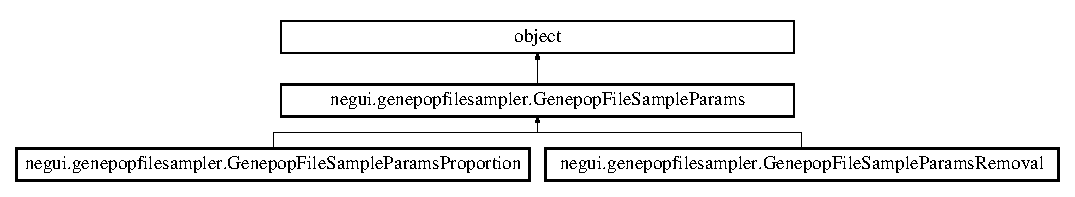
\includegraphics[height=2.193212cm]{classnegui_1_1genepopfilesampler_1_1GenepopFileSampleParams}
\end{center}
\end{figure}
\subsection*{Public Member Functions}
\begin{DoxyCompactItemize}
\item 
def \hyperlink{classnegui_1_1genepopfilesampler_1_1GenepopFileSampleParams_adb4c66f2bffa0a2eca84ed3dd3bc6385}{\+\_\+\+\_\+init\+\_\+\+\_\+} (self, li\+\_\+population\+\_\+numbers, s\+\_\+population\+\_\+subsample\+\_\+name=\char`\"{}population\+\_\+numbers\char`\"{})
\item 
def {\bfseries population\+\_\+numbers} (self)\hypertarget{classnegui_1_1genepopfilesampler_1_1GenepopFileSampleParams_a5ecc667eef35a832923e5c4ce659cfe7}{}\label{classnegui_1_1genepopfilesampler_1_1GenepopFileSampleParams_a5ecc667eef35a832923e5c4ce659cfe7}

\item 
def {\bfseries population\+\_\+subsample\+\_\+name} (self)\hypertarget{classnegui_1_1genepopfilesampler_1_1GenepopFileSampleParams_ab3ae1c545edd5230e6c37db9507d0535}{}\label{classnegui_1_1genepopfilesampler_1_1GenepopFileSampleParams_ab3ae1c545edd5230e6c37db9507d0535}

\end{DoxyCompactItemize}


\subsection{Detailed Description}
\begin{DoxyVerb}Supporting objects for GenepopFileSampler instances,
proving the sampling parameters.  For example, for 
sampling by proportions, this object would provide
a list of proportions of which each population is to 
be sampled, and a number of replicates indicating how
many samples to take at each proportion.  Further,
These objects also supply a list of population numbers,
from the range 1,2,3,...,N of the genepop files N
populations
\end{DoxyVerb}
 

Definition at line 89 of file genepopfilesampler.\+py.



\subsection{Constructor \& Destructor Documentation}
\index{negui\+::genepopfilesampler\+::\+Genepop\+File\+Sample\+Params@{negui\+::genepopfilesampler\+::\+Genepop\+File\+Sample\+Params}!\+\_\+\+\_\+init\+\_\+\+\_\+@{\+\_\+\+\_\+init\+\_\+\+\_\+}}
\index{\+\_\+\+\_\+init\+\_\+\+\_\+@{\+\_\+\+\_\+init\+\_\+\+\_\+}!negui\+::genepopfilesampler\+::\+Genepop\+File\+Sample\+Params@{negui\+::genepopfilesampler\+::\+Genepop\+File\+Sample\+Params}}
\subsubsection[{\texorpdfstring{\+\_\+\+\_\+init\+\_\+\+\_\+(self, li\+\_\+population\+\_\+numbers, s\+\_\+population\+\_\+subsample\+\_\+name=""population\+\_\+numbers"")}{__init__(self, li_population_numbers, s_population_subsample_name="population_numbers")}}]{\setlength{\rightskip}{0pt plus 5cm}def negui.\+genepopfilesampler.\+Genepop\+File\+Sample\+Params.\+\_\+\+\_\+init\+\_\+\+\_\+ (
\begin{DoxyParamCaption}
\item[{}]{self, }
\item[{}]{li\+\_\+population\+\_\+numbers, }
\item[{}]{s\+\_\+population\+\_\+subsample\+\_\+name = {\ttfamily \char`\"{}population\+\_\+numbers\char`\"{}}}
\end{DoxyParamCaption}
)}\hypertarget{classnegui_1_1genepopfilesampler_1_1GenepopFileSampleParams_adb4c66f2bffa0a2eca84ed3dd3bc6385}{}\label{classnegui_1_1genepopfilesampler_1_1GenepopFileSampleParams_adb4c66f2bffa0a2eca84ed3dd3bc6385}
\begin{DoxyVerb}Param li_populations is a list of integers,
each of i of which refers to the ith population
in the genepop file as represented by a 
genepopfilemanager object
\end{DoxyVerb}
 

Definition at line 102 of file genepopfilesampler.\+py.


\begin{DoxyCode}
102                 s\_population\_subsample\_name=\textcolor{stringliteral}{"population\_numbers"} ):
103         \textcolor{stringliteral}{'''}
104 \textcolor{stringliteral}{        Param li\_populations is a list of integers,}
105 \textcolor{stringliteral}{        each of i of which refers to the ith population}
106 \textcolor{stringliteral}{        in the genepop file as represented by a }
107 \textcolor{stringliteral}{        genepopfilemanager object}
108 \textcolor{stringliteral}{        '''}
109         self.\hyperlink{classnegui_1_1genepopfilesampler_1_1GenepopFileSampleParams_a48dfd2df4eb75dbacdc8a274cd3323ad}{\_\_populationnumbers}=li\_population\_numbers
110         self.\hyperlink{classnegui_1_1genepopfilesampler_1_1GenepopFileSampleParams_ae03531d2c9d450d7f717816a06f3a08a}{\_\_populationsubsamplename}=s\_population\_subsample\_name
111         \textcolor{keywordflow}{return}
\end{DoxyCode}


The documentation for this class was generated from the following file\+:\begin{DoxyCompactItemize}
\item 
genepopfilesampler.\+py\end{DoxyCompactItemize}

\hypertarget{classnegui_1_1genepopfilesampler_1_1GenepopFileSampleParamsProportion}{}\section{negui.\+genepopfilesampler.\+Genepop\+File\+Sample\+Params\+Proportion Class Reference}
\label{classnegui_1_1genepopfilesampler_1_1GenepopFileSampleParamsProportion}\index{negui.\+genepopfilesampler.\+Genepop\+File\+Sample\+Params\+Proportion@{negui.\+genepopfilesampler.\+Genepop\+File\+Sample\+Params\+Proportion}}
Inheritance diagram for negui.\+genepopfilesampler.\+Genepop\+File\+Sample\+Params\+Proportion\+:\begin{figure}[H]
\begin{center}
\leavevmode
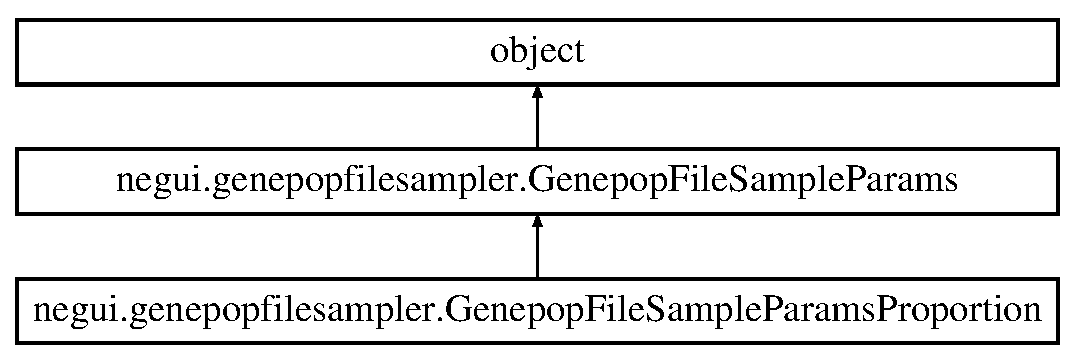
\includegraphics[height=3.000000cm]{classnegui_1_1genepopfilesampler_1_1GenepopFileSampleParamsProportion}
\end{center}
\end{figure}
\subsection*{Public Member Functions}
\begin{DoxyCompactItemize}
\item 
def \hyperlink{classnegui_1_1genepopfilesampler_1_1GenepopFileSampleParamsProportion_ab75eceef987c513501a5d55fb7ef3f7b}{\+\_\+\+\_\+init\+\_\+\+\_\+} (self, li\+\_\+population\+\_\+numbers, lf\+\_\+proportions, i\+\_\+replicates, s\+\_\+population\+\_\+subsample\+\_\+name=\char`\"{}population\+\_\+numbers\char`\"{}, s\+\_\+sample\+\_\+tag\+\_\+base=None)
\item 
def {\bfseries proportions} (self)\hypertarget{classnegui_1_1genepopfilesampler_1_1GenepopFileSampleParamsProportion_a0b564f11df13b230af1cb7a86e1376e1}{}\label{classnegui_1_1genepopfilesampler_1_1GenepopFileSampleParamsProportion_a0b564f11df13b230af1cb7a86e1376e1}

\end{DoxyCompactItemize}


\subsection{Detailed Description}


Definition at line 377 of file genepopfilesampler.\+py.



\subsection{Constructor \& Destructor Documentation}
\index{negui\+::genepopfilesampler\+::\+Genepop\+File\+Sample\+Params\+Proportion@{negui\+::genepopfilesampler\+::\+Genepop\+File\+Sample\+Params\+Proportion}!\+\_\+\+\_\+init\+\_\+\+\_\+@{\+\_\+\+\_\+init\+\_\+\+\_\+}}
\index{\+\_\+\+\_\+init\+\_\+\+\_\+@{\+\_\+\+\_\+init\+\_\+\+\_\+}!negui\+::genepopfilesampler\+::\+Genepop\+File\+Sample\+Params\+Proportion@{negui\+::genepopfilesampler\+::\+Genepop\+File\+Sample\+Params\+Proportion}}
\subsubsection[{\texorpdfstring{\+\_\+\+\_\+init\+\_\+\+\_\+(self, li\+\_\+population\+\_\+numbers, lf\+\_\+proportions, i\+\_\+replicates, s\+\_\+population\+\_\+subsample\+\_\+name=""population\+\_\+numbers"", s\+\_\+sample\+\_\+tag\+\_\+base=\+None)}{__init__(self, li_population_numbers, lf_proportions, i_replicates, s_population_subsample_name="population_numbers", s_sample_tag_base=None)}}]{\setlength{\rightskip}{0pt plus 5cm}def negui.\+genepopfilesampler.\+Genepop\+File\+Sample\+Params\+Proportion.\+\_\+\+\_\+init\+\_\+\+\_\+ (
\begin{DoxyParamCaption}
\item[{}]{self, }
\item[{}]{li\+\_\+population\+\_\+numbers, }
\item[{}]{lf\+\_\+proportions, }
\item[{}]{i\+\_\+replicates, }
\item[{}]{s\+\_\+population\+\_\+subsample\+\_\+name = {\ttfamily \char`\"{}population\+\_\+numbers\char`\"{}}, }
\item[{}]{s\+\_\+sample\+\_\+tag\+\_\+base = {\ttfamily None}}
\end{DoxyParamCaption}
)}\hypertarget{classnegui_1_1genepopfilesampler_1_1GenepopFileSampleParamsProportion_ab75eceef987c513501a5d55fb7ef3f7b}{}\label{classnegui_1_1genepopfilesampler_1_1GenepopFileSampleParamsProportion_ab75eceef987c513501a5d55fb7ef3f7b}
\begin{DoxyVerb}param li_populations, list of ints, which pops to sample (see remarks, parant class )
param lf_proportions, list of floats, each pop sampled at each of these proportions
param i_replicates, one integer, each pop sampled at each proportion this many times
GenepopFileSampleParams.__init__( self, li_populations )
\end{DoxyVerb}
 

Definition at line 382 of file genepopfilesampler.\+py.


\begin{DoxyCode}
382             s\_sample\_tag\_base=\textcolor{keywordtype}{None} ):
383 
384         \textcolor{stringliteral}{'''}
385 \textcolor{stringliteral}{        param li\_populations, list of ints, which pops to sample (see remarks, parant class )}
386 \textcolor{stringliteral}{        param lf\_proportions, list of floats, each pop sampled at each of these proportions}
387 \textcolor{stringliteral}{        param i\_replicates, one integer, each pop sampled at each proportion this many times}
388 \textcolor{stringliteral}{        GenepopFileSampleParams.\_\_init\_\_( self, li\_populations )}
389 \textcolor{stringliteral}{        '''}
390 
391         GenepopFileSampleParams.\_\_init\_\_(self, li\_population\_numbers=li\_population\_numbers, 
392                                             s\_population\_subsample\_name=s\_population\_subsample\_name,
393                                             s\_sample\_tag\_base=s\_sample\_tag\_base,
394                                             i\_replicates=i\_replicates )
395         self.\hyperlink{classnegui_1_1genepopfilesampler_1_1GenepopFileSampleParamsProportion_aa8dd8cef783da4e9bdb7c550e56382fd}{\_\_proportions}=lf\_proportions
396         \textcolor{keywordflow}{return}
\end{DoxyCode}


The documentation for this class was generated from the following file\+:\begin{DoxyCompactItemize}
\item 
genepopfilesampler.\+py\end{DoxyCompactItemize}

\hypertarget{classnegui_1_1genepopfilesampler_1_1GenepopFileSampleParamsRemoval}{}\section{negui.\+genepopfilesampler.\+Genepop\+File\+Sample\+Params\+Removal Class Reference}
\label{classnegui_1_1genepopfilesampler_1_1GenepopFileSampleParamsRemoval}\index{negui.\+genepopfilesampler.\+Genepop\+File\+Sample\+Params\+Removal@{negui.\+genepopfilesampler.\+Genepop\+File\+Sample\+Params\+Removal}}
Inheritance diagram for negui.\+genepopfilesampler.\+Genepop\+File\+Sample\+Params\+Removal\+:\begin{figure}[H]
\begin{center}
\leavevmode
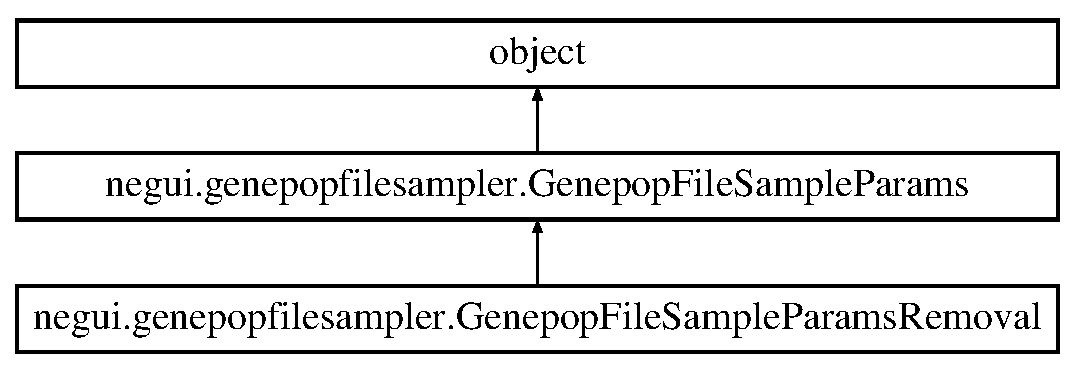
\includegraphics[height=3.000000cm]{classnegui_1_1genepopfilesampler_1_1GenepopFileSampleParamsRemoval}
\end{center}
\end{figure}
\subsection*{Public Member Functions}
\begin{DoxyCompactItemize}
\item 
def \hyperlink{classnegui_1_1genepopfilesampler_1_1GenepopFileSampleParamsRemoval_a4eb7dd24a224c024d50c3bc7f99fe283}{\+\_\+\+\_\+init\+\_\+\+\_\+} (self, li\+\_\+population\+\_\+numbers, li\+\_\+n\+\_\+to\+\_\+remove, i\+\_\+replicates, s\+\_\+population\+\_\+subsample\+\_\+name=\char`\"{}poplulation\+\_\+numbers\char`\"{}, b\+\_\+do\+\_\+all\+\_\+combos\+\_\+when\+\_\+n\+\_\+equals\+\_\+one=True)
\item 
def {\bfseries n\+\_\+to\+\_\+remove} (self)\hypertarget{classnegui_1_1genepopfilesampler_1_1GenepopFileSampleParamsRemoval_a7621d89a31284b0d6d8b49598eb1860d}{}\label{classnegui_1_1genepopfilesampler_1_1GenepopFileSampleParamsRemoval_a7621d89a31284b0d6d8b49598eb1860d}

\item 
def {\bfseries replicates} (self)\hypertarget{classnegui_1_1genepopfilesampler_1_1GenepopFileSampleParamsRemoval_a78561df77c45519715a9dd14bdfd23a0}{}\label{classnegui_1_1genepopfilesampler_1_1GenepopFileSampleParamsRemoval_a78561df77c45519715a9dd14bdfd23a0}

\item 
def {\bfseries do\+\_\+all\+\_\+combos\+\_\+when\+\_\+n\+\_\+equals\+\_\+one} (self)\hypertarget{classnegui_1_1genepopfilesampler_1_1GenepopFileSampleParamsRemoval_a6999b2175c9660123c62495ff155ad08}{}\label{classnegui_1_1genepopfilesampler_1_1GenepopFileSampleParamsRemoval_a6999b2175c9660123c62495ff155ad08}

\end{DoxyCompactItemize}


\subsection{Detailed Description}
\begin{DoxyVerb}Parameters for sampling scheme such that for each population
we randomly remove N of the M individuals, removing all M where
N>=M, repeating i_replicate times. 

When the b_do_all_combos_when_n_equals_one flag in __init__ is
set to True (the default), we treat N=1 differently, and 
exhaust all possible removals -- i.e, in each pop_i 
of size M_i, removing each N where N=1,2,3...M_i.
\end{DoxyVerb}
 

Definition at line 158 of file genepopfilesampler.\+py.



\subsection{Constructor \& Destructor Documentation}
\index{negui\+::genepopfilesampler\+::\+Genepop\+File\+Sample\+Params\+Removal@{negui\+::genepopfilesampler\+::\+Genepop\+File\+Sample\+Params\+Removal}!\+\_\+\+\_\+init\+\_\+\+\_\+@{\+\_\+\+\_\+init\+\_\+\+\_\+}}
\index{\+\_\+\+\_\+init\+\_\+\+\_\+@{\+\_\+\+\_\+init\+\_\+\+\_\+}!negui\+::genepopfilesampler\+::\+Genepop\+File\+Sample\+Params\+Removal@{negui\+::genepopfilesampler\+::\+Genepop\+File\+Sample\+Params\+Removal}}
\subsubsection[{\texorpdfstring{\+\_\+\+\_\+init\+\_\+\+\_\+(self, li\+\_\+population\+\_\+numbers, li\+\_\+n\+\_\+to\+\_\+remove, i\+\_\+replicates, s\+\_\+population\+\_\+subsample\+\_\+name=""poplulation\+\_\+numbers"", b\+\_\+do\+\_\+all\+\_\+combos\+\_\+when\+\_\+n\+\_\+equals\+\_\+one=\+True)}{__init__(self, li_population_numbers, li_n_to_remove, i_replicates, s_population_subsample_name="poplulation_numbers", b_do_all_combos_when_n_equals_one=True)}}]{\setlength{\rightskip}{0pt plus 5cm}def negui.\+genepopfilesampler.\+Genepop\+File\+Sample\+Params\+Removal.\+\_\+\+\_\+init\+\_\+\+\_\+ (
\begin{DoxyParamCaption}
\item[{}]{self, }
\item[{}]{li\+\_\+population\+\_\+numbers, }
\item[{}]{li\+\_\+n\+\_\+to\+\_\+remove, }
\item[{}]{i\+\_\+replicates, }
\item[{}]{s\+\_\+population\+\_\+subsample\+\_\+name = {\ttfamily \char`\"{}poplulation\+\_\+numbers\char`\"{}}, }
\item[{}]{b\+\_\+do\+\_\+all\+\_\+combos\+\_\+when\+\_\+n\+\_\+equals\+\_\+one = {\ttfamily True}}
\end{DoxyParamCaption}
)}\hypertarget{classnegui_1_1genepopfilesampler_1_1GenepopFileSampleParamsRemoval_a4eb7dd24a224c024d50c3bc7f99fe283}{}\label{classnegui_1_1genepopfilesampler_1_1GenepopFileSampleParamsRemoval_a4eb7dd24a224c024d50c3bc7f99fe283}
\begin{DoxyVerb}param li_population_numbers, list of ints, see parent class
param li_n_to_remove, list of ints, indicating, for each pop, randomly 
      remove n individuals
param i_replicates, for each i_n, repeat i_replicates times
param s_population_subsample_name, see parent class
param b_do_all_combos_when_n_equals_one -- if true treat n=1 differently,
      by repeating a remove-one-indiv for each indiv in each pop.
\end{DoxyVerb}
 

Definition at line 176 of file genepopfilesampler.\+py.


\begin{DoxyCode}
176             b\_do\_all\_combos\_when\_n\_equals\_one=\textcolor{keyword}{True} ):
177         \textcolor{stringliteral}{'''}
178 \textcolor{stringliteral}{        param li\_population\_numbers, list of ints, see parent class}
179 \textcolor{stringliteral}{        param li\_n\_to\_remove, list of ints, indicating, for each pop, randomly }
180 \textcolor{stringliteral}{              remove n individuals}
181 \textcolor{stringliteral}{        param i\_replicates, for each i\_n, repeat i\_replicates times}
182 \textcolor{stringliteral}{        param s\_population\_subsample\_name, see parent class}
183 \textcolor{stringliteral}{        param b\_do\_all\_combos\_when\_n\_equals\_one -- if true treat n=1 differently,}
184 \textcolor{stringliteral}{              by repeating a remove-one-indiv for each indiv in each pop.}
185 \textcolor{stringliteral}{        '''}
186 
187         GenepopFileSampleParams.\_\_init\_\_(self, 
188                     li\_population\_numbers=li\_population\_numbers, 
189                     s\_population\_subsample\_name=s\_population\_subsample\_name )
190 
191         self.\hyperlink{classnegui_1_1genepopfilesampler_1_1GenepopFileSampleParamsRemoval_a23d601163d8118b7af9acf6acf78eecf}{\_\_n\_to\_remove}=li\_n\_to\_remove
192         self.\hyperlink{classnegui_1_1genepopfilesampler_1_1GenepopFileSampleParamsRemoval_ae2a4f45ac6b5377f749dc84a560dbf01}{\_\_replicates}=i\_replicates
193         self.\hyperlink{classnegui_1_1genepopfilesampler_1_1GenepopFileSampleParamsRemoval_a24a47d9cdac499238a1368dcc626e8a3}{\_\_do\_all\_combos\_when\_n\_equals\_one}=
      b\_do\_all\_combos\_when\_n\_equals\_one
194         \textcolor{keywordflow}{return}
\end{DoxyCode}


The documentation for this class was generated from the following file\+:\begin{DoxyCompactItemize}
\item 
genepopfilesampler.\+py\end{DoxyCompactItemize}

\hypertarget{classnegui_1_1genepopfilesampler_1_1GenepopFileSampler}{}\section{negui.\+genepopfilesampler.\+Genepop\+File\+Sampler Class Reference}
\label{classnegui_1_1genepopfilesampler_1_1GenepopFileSampler}\index{negui.\+genepopfilesampler.\+Genepop\+File\+Sampler@{negui.\+genepopfilesampler.\+Genepop\+File\+Sampler}}
Inheritance diagram for negui.\+genepopfilesampler.\+Genepop\+File\+Sampler\+:\begin{figure}[H]
\begin{center}
\leavevmode
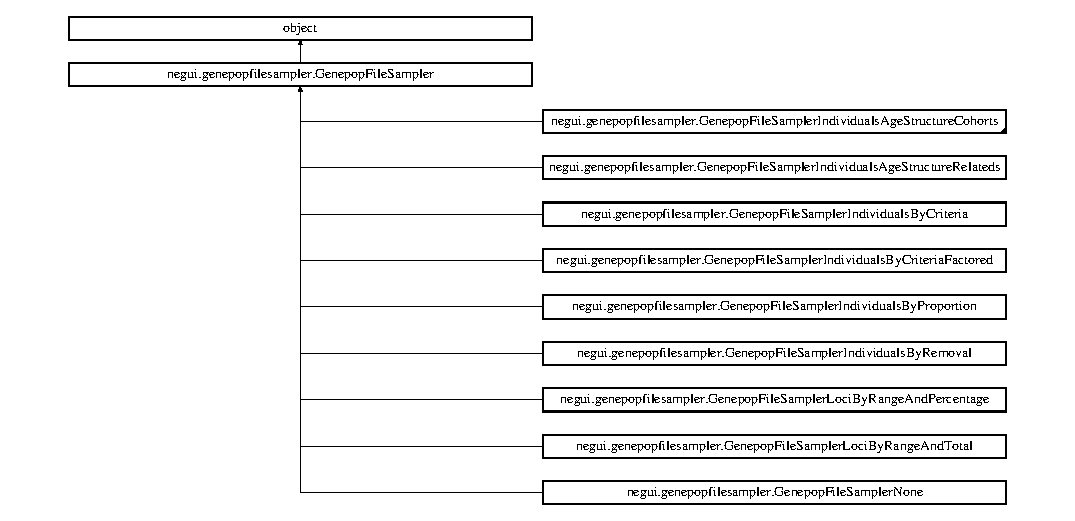
\includegraphics[height=5.957447cm]{classnegui_1_1genepopfilesampler_1_1GenepopFileSampler}
\end{center}
\end{figure}
\subsection*{Public Member Functions}
\begin{DoxyCompactItemize}
\item 
def {\bfseries \+\_\+\+\_\+init\+\_\+\+\_\+} (self, o\+\_\+genepopfilemanager, o\+\_\+genepopfilesampleparams)\hypertarget{classnegui_1_1genepopfilesampler_1_1GenepopFileSampler_abcaee019cd11b009568dde7fa2e94341}{}\label{classnegui_1_1genepopfilesampler_1_1GenepopFileSampler_abcaee019cd11b009568dde7fa2e94341}

\item 
def {\bfseries filemanager} (self)\hypertarget{classnegui_1_1genepopfilesampler_1_1GenepopFileSampler_a58431ed64951ef4a3cf813c9ee2624b3}{}\label{classnegui_1_1genepopfilesampler_1_1GenepopFileSampler_a58431ed64951ef4a3cf813c9ee2624b3}

\item 
def {\bfseries sampleparams} (self)\hypertarget{classnegui_1_1genepopfilesampler_1_1GenepopFileSampler_ad48f60ff378a777538a886b058eb0e00}{}\label{classnegui_1_1genepopfilesampler_1_1GenepopFileSampler_ad48f60ff378a777538a886b058eb0e00}

\end{DoxyCompactItemize}


\subsection{Detailed Description}
\begin{DoxyVerb}Class GenepopFileSampler instances operate on GenepopFileManager objects,
adding subsamples to the GenepopFileManager's subsample according to one of
mulitple sampling schemes.  It's chief motivation is a need to enccapsulate 
a session in which a large number of samples need to be taken from a single
genepop file, according to one of various possible sampling schemes.
\end{DoxyVerb}
 

Definition at line 87 of file genepopfilesampler.\+py.



The documentation for this class was generated from the following file\+:\begin{DoxyCompactItemize}
\item 
genepopfilesampler.\+py\end{DoxyCompactItemize}

\hypertarget{classnegui_1_1genepopfilesampler_1_1GenepopFileSamplerIndividualsByProportion}{}\section{negui.\+genepopfilesampler.\+Genepop\+File\+Sampler\+Individuals\+By\+Proportion Class Reference}
\label{classnegui_1_1genepopfilesampler_1_1GenepopFileSamplerIndividualsByProportion}\index{negui.\+genepopfilesampler.\+Genepop\+File\+Sampler\+Individuals\+By\+Proportion@{negui.\+genepopfilesampler.\+Genepop\+File\+Sampler\+Individuals\+By\+Proportion}}
Inheritance diagram for negui.\+genepopfilesampler.\+Genepop\+File\+Sampler\+Individuals\+By\+Proportion\+:\begin{figure}[H]
\begin{center}
\leavevmode
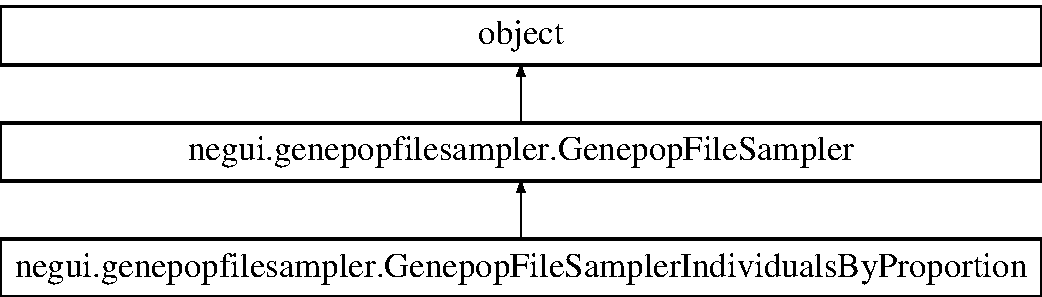
\includegraphics[height=3.000000cm]{classnegui_1_1genepopfilesampler_1_1GenepopFileSamplerIndividualsByProportion}
\end{center}
\end{figure}
\subsection*{Public Member Functions}
\begin{DoxyCompactItemize}
\item 
def {\bfseries \+\_\+\+\_\+init\+\_\+\+\_\+} (self, o\+\_\+genepopfilemanager, o\+\_\+genepopfilesampleparams)\hypertarget{classnegui_1_1genepopfilesampler_1_1GenepopFileSamplerIndividualsByProportion_a1bc0babcecf6bbca34259328cae53b97}{}\label{classnegui_1_1genepopfilesampler_1_1GenepopFileSamplerIndividualsByProportion_a1bc0babcecf6bbca34259328cae53b97}

\item 
def \hyperlink{classnegui_1_1genepopfilesampler_1_1GenepopFileSamplerIndividualsByProportion_ad8170ea6661afa7bff72d484372209e3}{do\+Sample} (self)
\end{DoxyCompactItemize}


\subsection{Detailed Description}
\begin{DoxyVerb}GenepopFileManager object that samples the individuals in each population
according one or more proportions (percentages).
\end{DoxyVerb}
 

Definition at line 1356 of file genepopfilesampler.\+py.



\subsection{Member Function Documentation}
\index{negui\+::genepopfilesampler\+::\+Genepop\+File\+Sampler\+Individuals\+By\+Proportion@{negui\+::genepopfilesampler\+::\+Genepop\+File\+Sampler\+Individuals\+By\+Proportion}!do\+Sample@{do\+Sample}}
\index{do\+Sample@{do\+Sample}!negui\+::genepopfilesampler\+::\+Genepop\+File\+Sampler\+Individuals\+By\+Proportion@{negui\+::genepopfilesampler\+::\+Genepop\+File\+Sampler\+Individuals\+By\+Proportion}}
\subsubsection[{\texorpdfstring{do\+Sample(self)}{doSample(self)}}]{\setlength{\rightskip}{0pt plus 5cm}def negui.\+genepopfilesampler.\+Genepop\+File\+Sampler\+Individuals\+By\+Proportion.\+do\+Sample (
\begin{DoxyParamCaption}
\item[{}]{self}
\end{DoxyParamCaption}
)}\hypertarget{classnegui_1_1genepopfilesampler_1_1GenepopFileSamplerIndividualsByProportion_ad8170ea6661afa7bff72d484372209e3}{}\label{classnegui_1_1genepopfilesampler_1_1GenepopFileSamplerIndividualsByProportion_ad8170ea6661afa7bff72d484372209e3}
\begin{DoxyVerb}as of Mon Jul 11 20:17:02 MDT 2016, for simplicity, the GenepopFileManager subsampling
defs that subsample individuals or loci, do so across all populations,
so that the subset of populations given by this objects member sampleparams property 
"population_numbers", will only be applied as a filter when writeGenePopFile (or printGenePopFile)
is applied to this objects GenepopFileManager object (self.filemanager ). The call
to the GenepopFileManager.writeGenePopFile, will need to include among its args the 
population subsample name ( assigned as the GenepopFileSampleParams object's
member "population_subsample_name") 
\end{DoxyVerb}
 

Definition at line 1366 of file genepopfilesampler.\+py.


\begin{DoxyCode}
1366     \textcolor{keyword}{def }\hyperlink{classnegui_1_1genepopfilesampler_1_1GenepopFileSamplerIndividualsByProportion_ad8170ea6661afa7bff72d484372209e3}{doSample}( self ):
1367         \textcolor{stringliteral}{'''}
1368 \textcolor{stringliteral}{        as of Mon Jul 11 20:17:02 MDT 2016, for simplicity, the GenepopFileManager subsampling}
1369 \textcolor{stringliteral}{        defs that subsample individuals or loci, do so across all populations,}
1370 \textcolor{stringliteral}{        so that the subset of populations given by this objects member sampleparams property }
1371 \textcolor{stringliteral}{        "population\_numbers", will only be applied as a filter when writeGenePopFile (or printGenePopFile)}
1372 \textcolor{stringliteral}{        is applied to this objects GenepopFileManager object (self.filemanager ). The call}
1373 \textcolor{stringliteral}{        to the GenepopFileManager.writeGenePopFile, will need to include among its args the }
1374 \textcolor{stringliteral}{        population subsample name ( assigned as the GenepopFileSampleParams object's}
1375 \textcolor{stringliteral}{        member "population\_subsample\_name") }
1376 \textcolor{stringliteral}{        '''}
1377 
1378         self.filemanager.subsamplePopulationsByList( self.sampleparams.population\_numbers, 
1379                 s\_subsample\_tag=self.sampleparams.population\_subsample\_name )
1380 
1381         lf\_proportions=self.sampleparams.proportions
1382         i\_total\_replicates=self.sampleparams.replicates
1383 
1384         \textcolor{keywordflow}{for} f\_proportion \textcolor{keywordflow}{in} lf\_proportions:
1385             \textcolor{keywordflow}{for} i\_replicate\_number \textcolor{keywordflow}{in} range( i\_total\_replicates ):
1386 
1387                 s\_subsampletag=\textcolor{keywordtype}{None}
1388 
1389                 \textcolor{keywordflow}{if} self.sampleparams.sample\_tag \textcolor{keywordflow}{is} \textcolor{keywordflow}{not} \textcolor{keywordtype}{None}:
1390                     s\_subsampletag=self.sampleparams.sample\_tag
1391                 \textcolor{keywordflow}{else}:
1392                     \textcolor{comment}{#standardized subsample tag uses the proportion and the rep number:}
1393                     \textcolor{comment}{#note that the "." char delimiter will need to be replaced by a diff}
1394                     \textcolor{comment}{#char when using this tag to name input or output file names for}
1395                     \textcolor{comment}{#NeEstimator (which truncates filenames using pattern .* for some of }
1396                     \textcolor{comment}{#its output files)}
1397                     s\_subsampletag=make\_subsample\_tag(  f\_proportion, i\_replicate\_number , 
      SCHEME\_PROPORTION )
1398                 \textcolor{comment}{#end if tag exists use it else make one}
1399 
1400                 self.filemanager.subsampleIndividualsRandomlyByProportion( f\_proportion, s\_subsampletag ) 
1401             \textcolor{comment}{#end for each replicate number  }
1402         \textcolor{comment}{#end for each proportion}
1403         \textcolor{keywordflow}{return}
1404 \textcolor{comment}{#end class GenepopFileSamplerIndividualsByProportion}
1405 
\end{DoxyCode}


The documentation for this class was generated from the following file\+:\begin{DoxyCompactItemize}
\item 
genepopfilesampler.\+py\end{DoxyCompactItemize}

\hypertarget{classnegui_1_1genepopfilesampler_1_1GenepopFileSamplerIndividualsByRemoval}{}\section{negui.\+genepopfilesampler.\+Genepop\+File\+Sampler\+Individuals\+By\+Removal Class Reference}
\label{classnegui_1_1genepopfilesampler_1_1GenepopFileSamplerIndividualsByRemoval}\index{negui.\+genepopfilesampler.\+Genepop\+File\+Sampler\+Individuals\+By\+Removal@{negui.\+genepopfilesampler.\+Genepop\+File\+Sampler\+Individuals\+By\+Removal}}
Inheritance diagram for negui.\+genepopfilesampler.\+Genepop\+File\+Sampler\+Individuals\+By\+Removal\+:\begin{figure}[H]
\begin{center}
\leavevmode
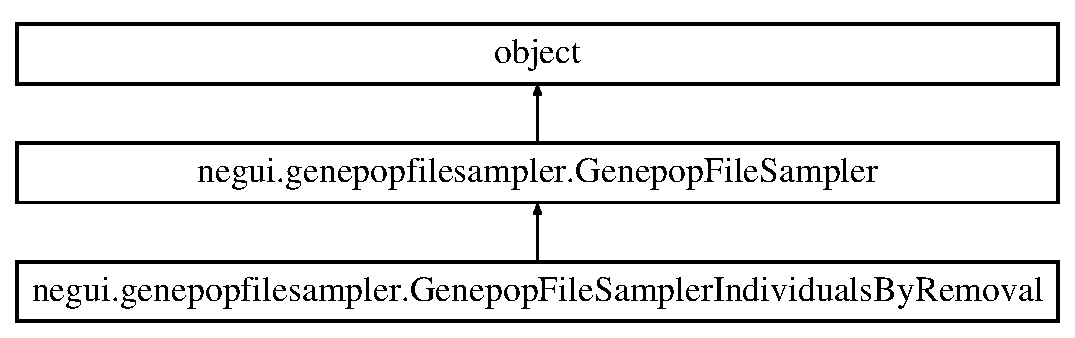
\includegraphics[height=3.000000cm]{classnegui_1_1genepopfilesampler_1_1GenepopFileSamplerIndividualsByRemoval}
\end{center}
\end{figure}
\subsection*{Public Member Functions}
\begin{DoxyCompactItemize}
\item 
def {\bfseries \+\_\+\+\_\+init\+\_\+\+\_\+} (self, o\+\_\+genepopfilemanager, o\+\_\+genepopfilesampleparams)\hypertarget{classnegui_1_1genepopfilesampler_1_1GenepopFileSamplerIndividualsByRemoval_aeba1258d811dd266cb3378212a4a1926}{}\label{classnegui_1_1genepopfilesampler_1_1GenepopFileSamplerIndividualsByRemoval_aeba1258d811dd266cb3378212a4a1926}

\item 
def {\bfseries do\+Sample} (self)\hypertarget{classnegui_1_1genepopfilesampler_1_1GenepopFileSamplerIndividualsByRemoval_a89dd3d276b9f089ac4c46dd844e7a848}{}\label{classnegui_1_1genepopfilesampler_1_1GenepopFileSamplerIndividualsByRemoval_a89dd3d276b9f089ac4c46dd844e7a848}

\end{DoxyCompactItemize}


\subsection{Detailed Description}
\begin{DoxyVerb}GenepopFileSampler object that samples individuals in each population
according to an N-removal scheme, that is, by removing N individuals 
randomly from the population, some M number of times, for some list of Ns
\end{DoxyVerb}
 

Definition at line 1406 of file genepopfilesampler.\+py.



The documentation for this class was generated from the following file\+:\begin{DoxyCompactItemize}
\item 
genepopfilesampler.\+py\end{DoxyCompactItemize}

\hypertarget{classnegui_1_1pgutilityclasses_1_1independantProcessGroup}{}\section{negui.\+pgutilityclasses.\+independant\+Process\+Group Class Reference}
\label{classnegui_1_1pgutilityclasses_1_1independantProcessGroup}\index{negui.\+pgutilityclasses.\+independant\+Process\+Group@{negui.\+pgutilityclasses.\+independant\+Process\+Group}}
Inheritance diagram for negui.\+pgutilityclasses.\+independant\+Process\+Group\+:\begin{figure}[H]
\begin{center}
\leavevmode
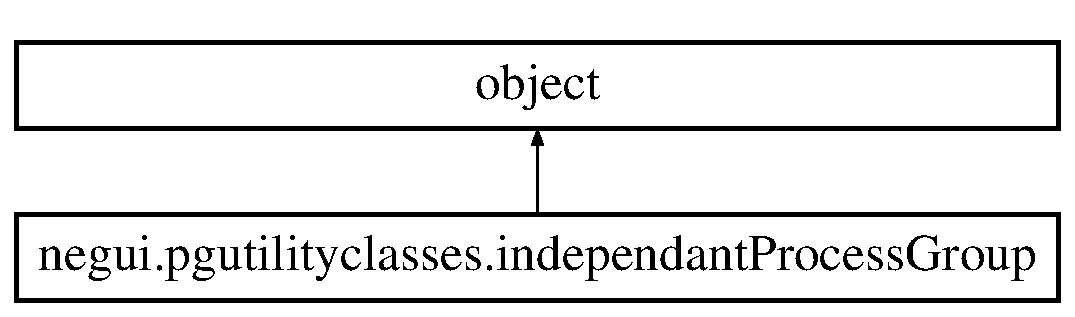
\includegraphics[height=2.000000cm]{classnegui_1_1pgutilityclasses_1_1independantProcessGroup}
\end{center}
\end{figure}
\subsection*{Public Member Functions}
\begin{DoxyCompactItemize}
\item 
def {\bfseries \+\_\+\+\_\+init\+\_\+\+\_\+} (self, lo\+\_\+processes=\mbox{[}$\,$\mbox{]})\hypertarget{classnegui_1_1pgutilityclasses_1_1independantProcessGroup_ac4c5c5b9bc52d8656cfb11ad6c3e83aa}{}\label{classnegui_1_1pgutilityclasses_1_1independantProcessGroup_ac4c5c5b9bc52d8656cfb11ad6c3e83aa}

\item 
def {\bfseries add\+Process} (self, o\+\_\+process)\hypertarget{classnegui_1_1pgutilityclasses_1_1independantProcessGroup_a746744058b90f36519d457f5fe9ff1fc}{}\label{classnegui_1_1pgutilityclasses_1_1independantProcessGroup_a746744058b90f36519d457f5fe9ff1fc}

\item 
def {\bfseries get\+Total\+Alive} (self)\hypertarget{classnegui_1_1pgutilityclasses_1_1independantProcessGroup_aa71d2b1111036aebcd9feb658797b819}{}\label{classnegui_1_1pgutilityclasses_1_1independantProcessGroup_aa71d2b1111036aebcd9feb658797b819}

\item 
def {\bfseries terminat\+All\+Processes} (self)\hypertarget{classnegui_1_1pgutilityclasses_1_1independantProcessGroup_a87e3c1396c5f4605f1ba7b46bde9acab}{}\label{classnegui_1_1pgutilityclasses_1_1independantProcessGroup_a87e3c1396c5f4605f1ba7b46bde9acab}

\end{DoxyCompactItemize}


\subsection{Detailed Description}
\begin{DoxyVerb}Simple convenience wrapper around a set of processes,
allowing calls into the instance to add a process,
or terminate all processes. This class is motivated
by implementing parallell replicate AgeStructureNe-inititated
simuPop simulations in a PGGuiSimuPop instance via
python's multiprocessing class, which apparently interacts
with simuPOP such that the multiprocessing.Pool and 
multiprocessing.Queue process managers do not create
simuPOP objects independant of each other.  This
necessitated using separately instantiated and started
multiprocessing.Process objects.  Because the typical
case will be to run y replicates using x processes, with
y>>x, then we need to manage the set of x processes, replacing
those finished with fresh processes.


All member processes are assumed to be completely 
independant of all others, so that any I/O messes 
caused by calling terminate() will not lock up 
the parent process
\end{DoxyVerb}
 

Definition at line 12 of file pgutilityclasses.\+py.



The documentation for this class was generated from the following file\+:\begin{DoxyCompactItemize}
\item 
pgutilityclasses.\+py\end{DoxyCompactItemize}

\hypertarget{classnegui_1_1pgguiutilities_1_1KeyCategoricalValueFrame}{}\section{negui.\+pgguiutilities.\+Key\+Categorical\+Value\+Frame Class Reference}
\label{classnegui_1_1pgguiutilities_1_1KeyCategoricalValueFrame}\index{negui.\+pgguiutilities.\+Key\+Categorical\+Value\+Frame@{negui.\+pgguiutilities.\+Key\+Categorical\+Value\+Frame}}
Inheritance diagram for negui.\+pgguiutilities.\+Key\+Categorical\+Value\+Frame\+:\begin{figure}[H]
\begin{center}
\leavevmode
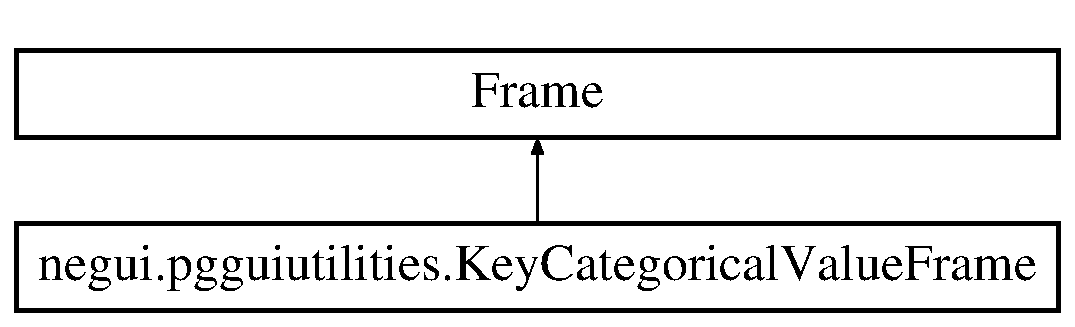
\includegraphics[height=2.000000cm]{classnegui_1_1pgguiutilities_1_1KeyCategoricalValueFrame}
\end{center}
\end{figure}
\subsection*{Public Member Functions}
\begin{DoxyCompactItemize}
\item 
def \hyperlink{classnegui_1_1pgguiutilities_1_1KeyCategoricalValueFrame_a8a88953e8615374aaddbb4347320e79c}{\+\_\+\+\_\+init\+\_\+\+\_\+} (self, s\+\_\+name, lq\+\_\+modes, i\+\_\+default\+\_\+mode\+\_\+number, o\+\_\+value\+\_\+type=None, o\+\_\+master=None, s\+\_\+associated\+\_\+attribute=None, o\+\_\+associated\+\_\+attribute\+\_\+object=None, def\+\_\+on\+\_\+button\+\_\+change=None, i\+\_\+labelwidth=15, b\+\_\+is\+\_\+enabled=True, s\+\_\+label\+\_\+justify=\textquotesingle{}right\textquotesingle{}, s\+\_\+buttons\+\_\+justify=\textquotesingle{}right\textquotesingle{}, s\+\_\+label\+\_\+name=None, b\+\_\+buttons\+\_\+in\+\_\+a\+\_\+row=False, b\+\_\+force\+\_\+disable=False, s\+\_\+tooltip=\char`\"{}\char`\"{})
\item 
def {\bfseries val} (self)\hypertarget{classnegui_1_1pgguiutilities_1_1KeyCategoricalValueFrame_a5d86db393ee3cf1e974f063a75b64b22}{}\label{classnegui_1_1pgguiutilities_1_1KeyCategoricalValueFrame_a5d86db393ee3cf1e974f063a75b64b22}

\item 
def {\bfseries val} (self)\hypertarget{classnegui_1_1pgguiutilities_1_1KeyCategoricalValueFrame_a5d86db393ee3cf1e974f063a75b64b22}{}\label{classnegui_1_1pgguiutilities_1_1KeyCategoricalValueFrame_a5d86db393ee3cf1e974f063a75b64b22}

\end{DoxyCompactItemize}


\subsection{Detailed Description}
\begin{DoxyVerb}Description

Revised KeyValueFrame
substituting a Radiobutton widget
for the entry box used in KeyValFrame\end{DoxyVerb}
 

Definition at line 689 of file pgguiutilities.\+py.



\subsection{Constructor \& Destructor Documentation}
\index{negui\+::pgguiutilities\+::\+Key\+Categorical\+Value\+Frame@{negui\+::pgguiutilities\+::\+Key\+Categorical\+Value\+Frame}!\+\_\+\+\_\+init\+\_\+\+\_\+@{\+\_\+\+\_\+init\+\_\+\+\_\+}}
\index{\+\_\+\+\_\+init\+\_\+\+\_\+@{\+\_\+\+\_\+init\+\_\+\+\_\+}!negui\+::pgguiutilities\+::\+Key\+Categorical\+Value\+Frame@{negui\+::pgguiutilities\+::\+Key\+Categorical\+Value\+Frame}}
\subsubsection[{\texorpdfstring{\+\_\+\+\_\+init\+\_\+\+\_\+(self, s\+\_\+name, lq\+\_\+modes, i\+\_\+default\+\_\+mode\+\_\+number, o\+\_\+value\+\_\+type=\+None, o\+\_\+master=\+None, s\+\_\+associated\+\_\+attribute=\+None, o\+\_\+associated\+\_\+attribute\+\_\+object=\+None, def\+\_\+on\+\_\+button\+\_\+change=\+None, i\+\_\+labelwidth=15, b\+\_\+is\+\_\+enabled=\+True, s\+\_\+label\+\_\+justify=\textquotesingle{}right\textquotesingle{}, s\+\_\+buttons\+\_\+justify=\textquotesingle{}right\textquotesingle{}, s\+\_\+label\+\_\+name=\+None, b\+\_\+buttons\+\_\+in\+\_\+a\+\_\+row=\+False, b\+\_\+force\+\_\+disable=\+False, s\+\_\+tooltip="""")}{__init__(self, s_name, lq_modes, i_default_mode_number, o_value_type=None, o_master=None, s_associated_attribute=None, o_associated_attribute_object=None, def_on_button_change=None, i_labelwidth=15, b_is_enabled=True, s_label_justify='right', s_buttons_justify='right', s_label_name=None, b_buttons_in_a_row=False, b_force_disable=False, s_tooltip="")}}]{\setlength{\rightskip}{0pt plus 5cm}def negui.\+pgguiutilities.\+Key\+Categorical\+Value\+Frame.\+\_\+\+\_\+init\+\_\+\+\_\+ (
\begin{DoxyParamCaption}
\item[{}]{self, }
\item[{}]{s\+\_\+name, }
\item[{}]{lq\+\_\+modes, }
\item[{}]{i\+\_\+default\+\_\+mode\+\_\+number, }
\item[{}]{o\+\_\+value\+\_\+type = {\ttfamily None}, }
\item[{}]{o\+\_\+master = {\ttfamily None}, }
\item[{}]{s\+\_\+associated\+\_\+attribute = {\ttfamily None}, }
\item[{}]{o\+\_\+associated\+\_\+attribute\+\_\+object = {\ttfamily None}, }
\item[{}]{def\+\_\+on\+\_\+button\+\_\+change = {\ttfamily None}, }
\item[{}]{i\+\_\+labelwidth = {\ttfamily 15}, }
\item[{}]{b\+\_\+is\+\_\+enabled = {\ttfamily True}, }
\item[{}]{s\+\_\+label\+\_\+justify = {\ttfamily \textquotesingle{}right\textquotesingle{}}, }
\item[{}]{s\+\_\+buttons\+\_\+justify = {\ttfamily \textquotesingle{}right\textquotesingle{}}, }
\item[{}]{s\+\_\+label\+\_\+name = {\ttfamily None}, }
\item[{}]{b\+\_\+buttons\+\_\+in\+\_\+a\+\_\+row = {\ttfamily False}, }
\item[{}]{b\+\_\+force\+\_\+disable = {\ttfamily False}, }
\item[{}]{s\+\_\+tooltip = {\ttfamily \char`\"{}\char`\"{}}}
\end{DoxyParamCaption}
)}\hypertarget{classnegui_1_1pgguiutilities_1_1KeyCategoricalValueFrame_a8a88953e8615374aaddbb4347320e79c}{}\label{classnegui_1_1pgguiutilities_1_1KeyCategoricalValueFrame_a8a88953e8615374aaddbb4347320e79c}
\begin{DoxyVerb}Param lq_modes, list of sequences, each a pair
    giving the mode label text, and its associated value
    assigned when it is the selected radio button
Param i_default_mode_number gives the ith (one-indexed)
    item in modes, that is to be the active button,
    and that gives the default value
Param o_value_type gives the python type for the values
    given in lq_modes value items.  Currently implemented
    for bool, int, float, and string.
Param o_master is the parent Tkinter object.
Param s_associated_attribute is the name of 
    attribute instance that can be accessed
    using "getattr", and that will be
    updated when the value is updated.
Param o_associated_attribute_object is the object whose attribute
    is to be unpdated when the value is updated.  If
    s_associated_attribute is not None, and this parameter
    is None, the attribute is presumed to be
    owned by the o_master object.
Param def_on_button_change, if not None, execute the def
    after updating both the value and the attribute (if any).
    This def is to have no passed params.
Param i_labelwidth gives the width the the Label widget.
Param s_label_justify gives Label widget "justify" value.
Param s_buttons_justify gives Radiobutten Widget text "justify" value.
currently not implemented (ttk radio button widgets are not
settable for justify and foreground, without using a syle map).
Param s_label_name, if not None, replaces s_name as the text for the label.
Param b_buttons_in_a_row, if False (default) all buttons are in a single column, if True,
then all buttons side by side in a single row
Param b_force_disable, if True, will override the b_is_enabled value and disable all entry 
      boxes
\end{DoxyVerb}
 

Definition at line 715 of file pgguiutilities.\+py.


\begin{DoxyCode}
715             s\_tooltip = \textcolor{stringliteral}{""} ):
716 
717         \textcolor{stringliteral}{"""}
718 \textcolor{stringliteral}{        Param lq\_modes, list of sequences, each a pair}
719 \textcolor{stringliteral}{            giving the mode label text, and its associated value}
720 \textcolor{stringliteral}{            assigned when it is the selected radio button}
721 \textcolor{stringliteral}{        Param i\_default\_mode\_number gives the ith (one-indexed)}
722 \textcolor{stringliteral}{            item in modes, that is to be the active button,}
723 \textcolor{stringliteral}{            and that gives the default value}
724 \textcolor{stringliteral}{        Param o\_value\_type gives the python type for the values}
725 \textcolor{stringliteral}{            given in lq\_modes value items.  Currently implemented}
726 \textcolor{stringliteral}{            for bool, int, float, and string.}
727 \textcolor{stringliteral}{        Param o\_master is the parent Tkinter object.}
728 \textcolor{stringliteral}{                Param s\_associated\_attribute is the name of }
729 \textcolor{stringliteral}{            attribute instance that can be accessed}
730 \textcolor{stringliteral}{            using "getattr", and that will be}
731 \textcolor{stringliteral}{            updated when the value is updated.}
732 \textcolor{stringliteral}{        Param o\_associated\_attribute\_object is the object whose attribute}
733 \textcolor{stringliteral}{            is to be unpdated when the value is updated.  If}
734 \textcolor{stringliteral}{            s\_associated\_attribute is not None, and this parameter}
735 \textcolor{stringliteral}{            is None, the attribute is presumed to be}
736 \textcolor{stringliteral}{            owned by the o\_master object.}
737 \textcolor{stringliteral}{        Param def\_on\_button\_change, if not None, execute the def}
738 \textcolor{stringliteral}{            after updating both the value and the attribute (if any).}
739 \textcolor{stringliteral}{            This def is to have no passed params.}
740 \textcolor{stringliteral}{        Param i\_labelwidth gives the width the the Label widget.}
741 \textcolor{stringliteral}{        Param s\_label\_justify gives Label widget "justify" value.}
742 \textcolor{stringliteral}{        Param s\_buttons\_justify gives Radiobutten Widget text "justify" value.}
743 \textcolor{stringliteral}{                currently not implemented (ttk radio button widgets are not}
744 \textcolor{stringliteral}{                settable for justify and foreground, without using a syle map).}
745 \textcolor{stringliteral}{        Param s\_label\_name, if not None, replaces s\_name as the text for the label.}
746 \textcolor{stringliteral}{        Param b\_buttons\_in\_a\_row, if False (default) all buttons are in a single column, if True,}
747 \textcolor{stringliteral}{                then all buttons side by side in a single row}
748 \textcolor{stringliteral}{        Param b\_force\_disable, if True, will override the b\_is\_enabled value and disable all entry }
749 \textcolor{stringliteral}{              boxes}
750 \textcolor{stringliteral}{        """}
751 
752         \textcolor{comment}{#TCL won't allow uppercase names for windows}
753         \textcolor{comment}{#(note that we save the name, case in-tact, in}
754         \textcolor{comment}{#member \_\_name:}
755         Frame.\_\_init\_\_( self, o\_master, name=s\_name.lower() )
756         self.\hyperlink{classnegui_1_1pgguiutilities_1_1KeyCategoricalValueFrame_ad0cd6c8b8265cb6b27efa7bbc5e23ae0}{\_\_master}=o\_master
757         self.\hyperlink{classnegui_1_1pgguiutilities_1_1KeyCategoricalValueFrame_ac743c18f66b310548e2dd0e3076b00c7}{\_\_value}=\textcolor{keywordtype}{None}
758         self.\hyperlink{classnegui_1_1pgguiutilities_1_1KeyCategoricalValueFrame_ae5f2855d8f22b4aa8f533023ac3e7fb4}{\_\_default\_mode\_number}=i\_default\_mode\_number
759         self.\hyperlink{classnegui_1_1pgguiutilities_1_1KeyCategoricalValueFrame_aadb3b6381c9159d303cd150e5a748096}{\_\_modes}=lq\_modes
760         self.\hyperlink{classnegui_1_1pgguiutilities_1_1KeyCategoricalValueFrame_a92a1947d6110ada3bd813cc8e84d84ad}{\_\_name}=s\_name
761         self.\hyperlink{classnegui_1_1pgguiutilities_1_1KeyCategoricalValueFrame_adf2c2370358ac051464aef108d75caa3}{\_\_lablewidth}=i\_labelwidth
762         self.\hyperlink{classnegui_1_1pgguiutilities_1_1KeyCategoricalValueFrame_a96cbcef967bddfd5035b827c0ae50c05}{\_\_labeljustify}=s\_label\_justify
763         self.\hyperlink{classnegui_1_1pgguiutilities_1_1KeyCategoricalValueFrame_a1fa18274aa53997c8b5fe446779b9a9d}{\_\_buttons\_justify}=s\_buttons\_justify
764         self.\hyperlink{classnegui_1_1pgguiutilities_1_1KeyCategoricalValueFrame_afb2be50b6de2bac5c96b9d73d93da416}{\_\_isenabled}=b\_is\_enabled
765         self.\hyperlink{classnegui_1_1pgguiutilities_1_1KeyCategoricalValueFrame_aa9b8f1b85890b51192559ff142d2360f}{\_\_associated\_attribute}=s\_associated\_attribute
766         self.\hyperlink{classnegui_1_1pgguiutilities_1_1KeyCategoricalValueFrame_a14174765fdf3479d1f7f09fe1deda5cf}{\_\_associated\_attribute\_object}=o\_associated\_attribute\_object
767         self.\hyperlink{classnegui_1_1pgguiutilities_1_1KeyCategoricalValueFrame_a0e462eacf72e4afb9711c917fe1c0d6a}{\_\_def\_on\_button\_change}=def\_on\_button\_change
768         self.\hyperlink{classnegui_1_1pgguiutilities_1_1KeyCategoricalValueFrame_a869087c9cc908de0226eec78cb4282bb}{\_\_put\_buttons\_in\_row}=b\_buttons\_in\_a\_row
769         self.\hyperlink{classnegui_1_1pgguiutilities_1_1KeyCategoricalValueFrame_aa1bb987386f2e559c6de976b745f185e}{\_\_current\_button\_value}=self.
      \hyperlink{classnegui_1_1pgguiutilities_1_1KeyCategoricalValueFrame_ab1e309b3e63c5c4a57d37d2a61f4e90d}{\_\_init\_current\_button\_val}( o\_value\_type )
770         self.\hyperlink{classnegui_1_1pgguiutilities_1_1KeyCategoricalValueFrame_a3a453ac47871c2f8b894442fd3ef5d07}{\_\_label\_name}=self.\hyperlink{classnegui_1_1pgguiutilities_1_1KeyCategoricalValueFrame_a92a1947d6110ada3bd813cc8e84d84ad}{\_\_name} \textcolor{keywordflow}{if} s\_label\_name \textcolor{keywordflow}{is} \textcolor{keywordtype}{None} \textcolor{keywordflow}{else} s\_label\_name
771         self.\hyperlink{classnegui_1_1pgguiutilities_1_1KeyCategoricalValueFrame_a01ea2795b9136b4fab5d6fe78dc2947d}{\_\_force\_disable}=b\_force\_disable
772         self.\hyperlink{classnegui_1_1pgguiutilities_1_1KeyCategoricalValueFrame_ae2f1424ab33f1ff0c9477dcf401748ca}{\_\_tooltip}=self.\hyperlink{classnegui_1_1pgguiutilities_1_1KeyCategoricalValueFrame_a3a453ac47871c2f8b894442fd3ef5d07}{\_\_label\_name} \textcolor{keywordflow}{if} s\_tooltip == \textcolor{stringliteral}{""} \textcolor{keywordflow}{else} s\_tooltip
773         self.\hyperlink{classnegui_1_1pgguiutilities_1_1KeyCategoricalValueFrame_ad2350dd7438d98d077c86e8295425ca0}{\_\_subframe}=\textcolor{keywordtype}{None}
774         self.\hyperlink{classnegui_1_1pgguiutilities_1_1KeyCategoricalValueFrame_a1e890256208ab06e21db468c7aed6bd8}{\_\_setup}()
\end{DoxyCode}


The documentation for this class was generated from the following file\+:\begin{DoxyCompactItemize}
\item 
pgguiutilities.\+py\end{DoxyCompactItemize}

\hypertarget{classnegui_1_1pgguiutilities_1_1KeyValFrame}{}\section{negui.\+pgguiutilities.\+Key\+Val\+Frame Class Reference}
\label{classnegui_1_1pgguiutilities_1_1KeyValFrame}\index{negui.\+pgguiutilities.\+Key\+Val\+Frame@{negui.\+pgguiutilities.\+Key\+Val\+Frame}}
Inheritance diagram for negui.\+pgguiutilities.\+Key\+Val\+Frame\+:\begin{figure}[H]
\begin{center}
\leavevmode
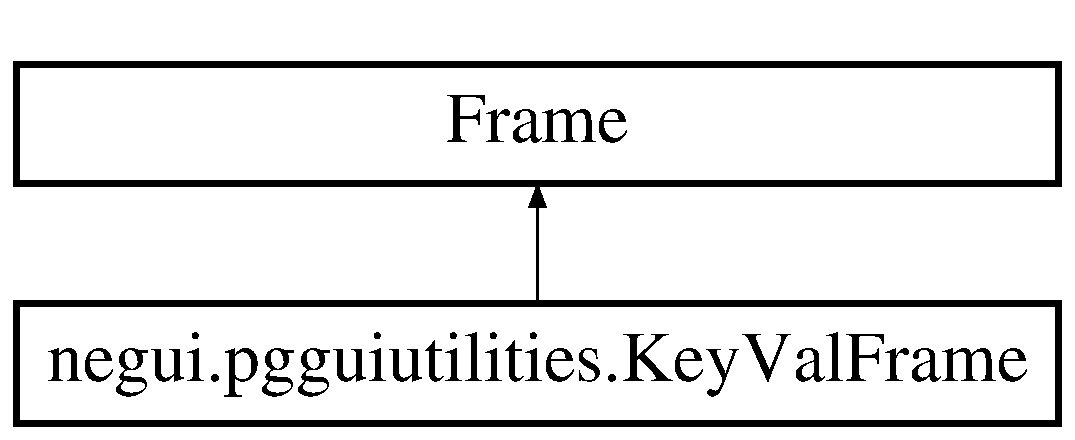
\includegraphics[height=2.000000cm]{classnegui_1_1pgguiutilities_1_1KeyValFrame}
\end{center}
\end{figure}
\subsection*{Public Member Functions}
\begin{DoxyCompactItemize}
\item 
def \hyperlink{classnegui_1_1pgguiutilities_1_1KeyValFrame_a9d507011f4523f708351c682b788f3e5}{\+\_\+\+\_\+init\+\_\+\+\_\+} (self, s\+\_\+name, v\+\_\+value, o\+\_\+type, v\+\_\+default\+\_\+value=None, o\+\_\+master=None, s\+\_\+associated\+\_\+attribute=None, o\+\_\+associated\+\_\+attribute\+\_\+object=None, i\+\_\+entrywidth=7, i\+\_\+labelwidth=15, b\+\_\+is\+\_\+enabled=True, s\+\_\+label\+\_\+justify=\textquotesingle{}right\textquotesingle{}, s\+\_\+entry\+\_\+justify=\textquotesingle{}right\textquotesingle{}, s\+\_\+button\+\_\+text=\textquotesingle{}Cmd\textquotesingle{}, def\+\_\+button\+\_\+command=None, def\+\_\+entry\+\_\+change\+\_\+command=None, type\+\_\+replaces\+\_\+none=float, s\+\_\+label\+\_\+name=None, i\+\_\+subframe\+\_\+padding=0, o\+\_\+validity\+\_\+tester=None, b\+\_\+force\+\_\+disable=False, s\+\_\+tooltip=None, b\+\_\+use\+\_\+list\+\_\+editor=False)
\item 
def {\bfseries val} (self)\hypertarget{classnegui_1_1pgguiutilities_1_1KeyValFrame_a735c32759de5e4519d15ec2511da6e4f}{}\label{classnegui_1_1pgguiutilities_1_1KeyValFrame_a735c32759de5e4519d15ec2511da6e4f}

\item 
def {\bfseries val} (self)\hypertarget{classnegui_1_1pgguiutilities_1_1KeyValFrame_a735c32759de5e4519d15ec2511da6e4f}{}\label{classnegui_1_1pgguiutilities_1_1KeyValFrame_a735c32759de5e4519d15ec2511da6e4f}

\end{DoxyCompactItemize}
\subsection*{Static Public Attributes}
\begin{DoxyCompactItemize}
\item 
bool {\bfseries V\+E\+R\+B\+O\+SE} = False\hypertarget{classnegui_1_1pgguiutilities_1_1KeyValFrame_a7ab96ae24edc45cf94f7cf10bc412557}{}\label{classnegui_1_1pgguiutilities_1_1KeyValFrame_a7ab96ae24edc45cf94f7cf10bc412557}

\end{DoxyCompactItemize}


\subsection{Detailed Description}
\begin{DoxyVerb}Description

Tkinter frame object that creates,
from left to right, a label, then 
one or more entry boxes, one entry box 
if the type is not "list", otherwise one 
entry box for each list item.

the instance stores changes in the value(s)
via callback on enter key.  The current
key/value state is delivered via a getValue

Optionally also updates a an attribute
in its master object, by name (using getattr)
whenever the entry box value is updated.

Optionally also places a button to the right
of the entry box or boxes, and calls a user-supplied
def whenever a box is updated.

2016_09_18

Revise by adding list editing functions.\end{DoxyVerb}
 

Definition at line 38 of file pgguiutilities.\+py.



\subsection{Constructor \& Destructor Documentation}
\index{negui\+::pgguiutilities\+::\+Key\+Val\+Frame@{negui\+::pgguiutilities\+::\+Key\+Val\+Frame}!\+\_\+\+\_\+init\+\_\+\+\_\+@{\+\_\+\+\_\+init\+\_\+\+\_\+}}
\index{\+\_\+\+\_\+init\+\_\+\+\_\+@{\+\_\+\+\_\+init\+\_\+\+\_\+}!negui\+::pgguiutilities\+::\+Key\+Val\+Frame@{negui\+::pgguiutilities\+::\+Key\+Val\+Frame}}
\subsubsection[{\texorpdfstring{\+\_\+\+\_\+init\+\_\+\+\_\+(self, s\+\_\+name, v\+\_\+value, o\+\_\+type, v\+\_\+default\+\_\+value=\+None, o\+\_\+master=\+None, s\+\_\+associated\+\_\+attribute=\+None, o\+\_\+associated\+\_\+attribute\+\_\+object=\+None, i\+\_\+entrywidth=7, i\+\_\+labelwidth=15, b\+\_\+is\+\_\+enabled=\+True, s\+\_\+label\+\_\+justify=\textquotesingle{}right\textquotesingle{}, s\+\_\+entry\+\_\+justify=\textquotesingle{}right\textquotesingle{}, s\+\_\+button\+\_\+text=\textquotesingle{}\+Cmd\textquotesingle{}, def\+\_\+button\+\_\+command=\+None, def\+\_\+entry\+\_\+change\+\_\+command=\+None, type\+\_\+replaces\+\_\+none=float, s\+\_\+label\+\_\+name=\+None, i\+\_\+subframe\+\_\+padding=0, o\+\_\+validity\+\_\+tester=\+None, b\+\_\+force\+\_\+disable=\+False, s\+\_\+tooltip=\+None, b\+\_\+use\+\_\+list\+\_\+editor=\+False)}{__init__(self, s_name, v_value, o_type, v_default_value=None, o_master=None, s_associated_attribute=None, o_associated_attribute_object=None, i_entrywidth=7, i_labelwidth=15, b_is_enabled=True, s_label_justify='right', s_entry_justify='right', s_button_text='Cmd', def_button_command=None, def_entry_change_command=None, type_replaces_none=float, s_label_name=None, i_subframe_padding=0, o_validity_tester=None, b_force_disable=False, s_tooltip=None, b_use_list_editor=False)}}]{\setlength{\rightskip}{0pt plus 5cm}def negui.\+pgguiutilities.\+Key\+Val\+Frame.\+\_\+\+\_\+init\+\_\+\+\_\+ (
\begin{DoxyParamCaption}
\item[{}]{self, }
\item[{}]{s\+\_\+name, }
\item[{}]{v\+\_\+value, }
\item[{}]{o\+\_\+type, }
\item[{}]{v\+\_\+default\+\_\+value = {\ttfamily None}, }
\item[{}]{o\+\_\+master = {\ttfamily None}, }
\item[{}]{s\+\_\+associated\+\_\+attribute = {\ttfamily None}, }
\item[{}]{o\+\_\+associated\+\_\+attribute\+\_\+object = {\ttfamily None}, }
\item[{}]{i\+\_\+entrywidth = {\ttfamily 7}, }
\item[{}]{i\+\_\+labelwidth = {\ttfamily 15}, }
\item[{}]{b\+\_\+is\+\_\+enabled = {\ttfamily True}, }
\item[{}]{s\+\_\+label\+\_\+justify = {\ttfamily \textquotesingle{}right\textquotesingle{}}, }
\item[{}]{s\+\_\+entry\+\_\+justify = {\ttfamily \textquotesingle{}right\textquotesingle{}}, }
\item[{}]{s\+\_\+button\+\_\+text = {\ttfamily \textquotesingle{}Cmd\textquotesingle{}}, }
\item[{}]{def\+\_\+button\+\_\+command = {\ttfamily None}, }
\item[{}]{def\+\_\+entry\+\_\+change\+\_\+command = {\ttfamily None}, }
\item[{}]{type\+\_\+replaces\+\_\+none = {\ttfamily float}, }
\item[{}]{s\+\_\+label\+\_\+name = {\ttfamily None}, }
\item[{}]{i\+\_\+subframe\+\_\+padding = {\ttfamily 0}, }
\item[{}]{o\+\_\+validity\+\_\+tester = {\ttfamily None}, }
\item[{}]{b\+\_\+force\+\_\+disable = {\ttfamily False}, }
\item[{}]{s\+\_\+tooltip = {\ttfamily None}, }
\item[{}]{b\+\_\+use\+\_\+list\+\_\+editor = {\ttfamily False}}
\end{DoxyParamCaption}
)}\hypertarget{classnegui_1_1pgguiutilities_1_1KeyValFrame_a9d507011f4523f708351c682b788f3e5}{}\label{classnegui_1_1pgguiutilities_1_1KeyValFrame_a9d507011f4523f708351c682b788f3e5}
\begin{DoxyVerb}Param s_name provides the label text.
param v_value is the current value to be set as the
value for this KeyValFrame instance.  Note
if the client suppliesa list, the type given
here will be that of each item in the list.
param o_type gives the type of the value, or, if
the value is a list, the type of the list items
(uniform type assumed for list items.
param v_default_value gives the value that will be used
if the v_value is a list and the list ListEditingSubframe
object is being used.  In this case, when the current v_value
has len==0, then when the user invokes the "extend" def
in the ListEditingSubframe instance, a new list appears with
the v_default value as the single list item.
Param o_master is the parent Tkinter object.
Param s_associated_attribute is the name of 
    attribute instance that can be accessed
    using "getattr", and that will be
    updated when the value is updated.
Param o_associated_attribute_object is the object whose attribute
    is to be unpdated when the value is updated.  If
    s_associated_attribute is not None, and this parameter
    is None, the attribute is presumed to be
    owned by the o_master object.
Param i_entrywidth gives the width of Entry widget(s).
Param i_labelwidth gives the width the the Label widget.
Param s_label_justify gives Label widget "justify" value.
Param s_entry_justify gives Entry Widget text "justify" value.
Param s_butten_text gives the Button Widget's text value.
Param def_button_command gives the def to set to the Button's "command" param.
Param def_entry_change_command gives a def to call when the value of an entry is changed.             
      it should be used when an attribute is asssociated with this object,
      and so is automatically updated, after wich some other action is required 
      (ex: Parent PGGuiSimuPop object needs to reconstiture the PGOutputSimuPop object 
      after this object updates its output basename attribute.
Param type_replaces_none: if a value is initially None, and the value is then updated, 
      this parameter.
      gives the type required for a valid value.
Param s_label_name, if supplied, replaces s_name as the text for the label.
Param i_subframe_padding gives the padding in pixels of the subframe inside its master frame
Param b_force_disable, if True, will cause all Entry objects to be disabled 
      in the def __make_entry
Param b_use_list_editor, if True, and if param v_value (see above) is passed as a list, 
      then a ListEditingSubframe object will be instantiated, allowing a GUI user to
      trim, extend, or assign one value to a range of list indices.
\end{DoxyVerb}
 

Definition at line 91 of file pgguiutilities.\+py.


\begin{DoxyCode}
91                     b\_use\_list\_editor=\textcolor{keyword}{False} ):
92         
93         \textcolor{stringliteral}{"""}
94 \textcolor{stringliteral}{        Param s\_name provides the label text.}
95 \textcolor{stringliteral}{        param v\_value is the current value to be set as the}
96 \textcolor{stringliteral}{                value for this KeyValFrame instance.  Note}
97 \textcolor{stringliteral}{                if the client suppliesa list, the type given}
98 \textcolor{stringliteral}{                here will be that of each item in the list.}
99 \textcolor{stringliteral}{        param o\_type gives the type of the value, or, if}
100 \textcolor{stringliteral}{                the value is a list, the type of the list items}
101 \textcolor{stringliteral}{                (uniform type assumed for list items.}
102 \textcolor{stringliteral}{        param v\_default\_value gives the value that will be used}
103 \textcolor{stringliteral}{                if the v\_value is a list and the list ListEditingSubframe}
104 \textcolor{stringliteral}{                object is being used.  In this case, when the current v\_value}
105 \textcolor{stringliteral}{                has len==0, then when the user invokes the "extend" def}
106 \textcolor{stringliteral}{                in the ListEditingSubframe instance, a new list appears with}
107 \textcolor{stringliteral}{                the v\_default value as the single list item.}
108 \textcolor{stringliteral}{        Param o\_master is the parent Tkinter object.}
109 \textcolor{stringliteral}{        Param s\_associated\_attribute is the name of }
110 \textcolor{stringliteral}{            attribute instance that can be accessed}
111 \textcolor{stringliteral}{            using "getattr", and that will be}
112 \textcolor{stringliteral}{            updated when the value is updated.}
113 \textcolor{stringliteral}{        Param o\_associated\_attribute\_object is the object whose attribute}
114 \textcolor{stringliteral}{            is to be unpdated when the value is updated.  If}
115 \textcolor{stringliteral}{            s\_associated\_attribute is not None, and this parameter}
116 \textcolor{stringliteral}{            is None, the attribute is presumed to be}
117 \textcolor{stringliteral}{            owned by the o\_master object.}
118 \textcolor{stringliteral}{        Param i\_entrywidth gives the width of Entry widget(s).}
119 \textcolor{stringliteral}{        Param i\_labelwidth gives the width the the Label widget.}
120 \textcolor{stringliteral}{        Param s\_label\_justify gives Label widget "justify" value.}
121 \textcolor{stringliteral}{        Param s\_entry\_justify gives Entry Widget text "justify" value.}
122 \textcolor{stringliteral}{        Param s\_butten\_text gives the Button Widget's text value.}
123 \textcolor{stringliteral}{        Param def\_button\_command gives the def to set to the Button's "command" param.}
124 \textcolor{stringliteral}{        Param def\_entry\_change\_command gives a def to call when the value of an entry is changed.           
        }
125 \textcolor{stringliteral}{              it should be used when an attribute is asssociated with this object,}
126 \textcolor{stringliteral}{              and so is automatically updated, after wich some other action is required }
127 \textcolor{stringliteral}{              (ex: Parent PGGuiSimuPop object needs to reconstiture the PGOutputSimuPop object }
128 \textcolor{stringliteral}{              after this object updates its output basename attribute.}
129 \textcolor{stringliteral}{        Param type\_replaces\_none: if a value is initially None, and the value is then updated, }
130 \textcolor{stringliteral}{              this parameter.}
131 \textcolor{stringliteral}{              gives the type required for a valid value.}
132 \textcolor{stringliteral}{        Param s\_label\_name, if supplied, replaces s\_name as the text for the label.}
133 \textcolor{stringliteral}{        Param i\_subframe\_padding gives the padding in pixels of the subframe inside its master frame}
134 \textcolor{stringliteral}{        Param b\_force\_disable, if True, will cause all Entry objects to be disabled }
135 \textcolor{stringliteral}{              in the def \_\_make\_entry}
136 \textcolor{stringliteral}{        Param b\_use\_list\_editor, if True, and if param v\_value (see above) is passed as a list, }
137 \textcolor{stringliteral}{              then a ListEditingSubframe object will be instantiated, allowing a GUI user to}
138 \textcolor{stringliteral}{              trim, extend, or assign one value to a range of list indices.}
139 \textcolor{stringliteral}{        """}
140 
141         \textcolor{comment}{#TCL won't allow uppercase names for windows}
142         \textcolor{comment}{#(note that we save the name, case in-tact, in}
143         \textcolor{comment}{#member \_\_name:}
144         Frame.\_\_init\_\_( self, o\_master, name=s\_name.lower() )
145         self.\hyperlink{classnegui_1_1pgguiutilities_1_1KeyValFrame_a59eae02effdbbbb9e3cf3e523639e8a8}{\_\_master}=o\_master
146         \textcolor{stringliteral}{'''}
147 \textcolor{stringliteral}{        This boolean var will be  reassigned}
148 \textcolor{stringliteral}{        if the client passed a list instead of an}
149 \textcolor{stringliteral}{        atomic type.  If true it will be reassigned}
150 \textcolor{stringliteral}{        in def \_\_store\_value:}
151 \textcolor{stringliteral}{        '''}
152         self.\hyperlink{classnegui_1_1pgguiutilities_1_1KeyValFrame_a2d79ed0f969cf5a4ce188cbece0828da}{\_\_orig\_value\_is\_list}=\textcolor{keyword}{False}
153         \textcolor{comment}{#Holds updated value, intiialized}
154         \textcolor{comment}{#in def \_\_store\_value}
155         self.\hyperlink{classnegui_1_1pgguiutilities_1_1KeyValFrame_a01709590a9e4395011a103b72a01159c}{\_\_value}=\textcolor{keywordtype}{None}
156         self.\hyperlink{classnegui_1_1pgguiutilities_1_1KeyValFrame_a7d3b0d0577b610c3fd6a3d1682906132}{\_\_default\_value}=v\_default\_value
157         self.\hyperlink{classnegui_1_1pgguiutilities_1_1KeyValFrame_a31219e9c697307bf80f807b3cbe8bb8b}{\_\_value\_type}=o\_type
158         self.\hyperlink{classnegui_1_1pgguiutilities_1_1KeyValFrame_abb469e367148bbf7c3fb27a523360016}{\_\_store\_value}( v\_value )
159         self.\hyperlink{classnegui_1_1pgguiutilities_1_1KeyValFrame_ab27ab044a7e5757c9311aef63dfb3b29}{\_\_last\_state}=self.\hyperlink{classnegui_1_1pgguiutilities_1_1KeyValFrame_a01709590a9e4395011a103b72a01159c}{\_\_value}
160         self.\hyperlink{classnegui_1_1pgguiutilities_1_1KeyValFrame_a08a3969c0310f969954e2b7fdd57a440}{\_\_name}=s\_name
161         self.\hyperlink{classnegui_1_1pgguiutilities_1_1KeyValFrame_a3b64ca90cda3d4031e6a637a51c5124e}{\_\_entrywidth}=i\_entrywidth
162         self.\hyperlink{classnegui_1_1pgguiutilities_1_1KeyValFrame_a3d346c456ee536a5404a2a9f94a7a341}{\_\_lablewidth}=i\_labelwidth
163         self.\hyperlink{classnegui_1_1pgguiutilities_1_1KeyValFrame_a0b4d970d0edce0eb0a7d5fd20c7da5b8}{\_\_labeljustify}=s\_label\_justify
164         self.\hyperlink{classnegui_1_1pgguiutilities_1_1KeyValFrame_a4d0dae8b1d43e1804727b3dfe1ba3383}{\_\_entryjustify}=s\_entry\_justify
165         self.\hyperlink{classnegui_1_1pgguiutilities_1_1KeyValFrame_a02d9e7225b8a2fb0eda398e68991e0e8}{\_\_isenabled}=b\_is\_enabled
166         self.\hyperlink{classnegui_1_1pgguiutilities_1_1KeyValFrame_a27b2ed9e7eeccc56397136ba42ccdaeb}{\_\_associated\_attribute}=s\_associated\_attribute
167         self.\hyperlink{classnegui_1_1pgguiutilities_1_1KeyValFrame_a73863067b82206c4f7d307be73ae5cd7}{\_\_associated\_attribute\_object}=o\_associated\_attribute\_object
168         self.\hyperlink{classnegui_1_1pgguiutilities_1_1KeyValFrame_abcbe36760268b6a6f2436527e3b45a77}{\_\_button\_text}=s\_button\_text
169         self.\hyperlink{classnegui_1_1pgguiutilities_1_1KeyValFrame_a0a4e9593fba1c3c0defc524ada661261}{\_\_button\_command}=def\_button\_command
170         self.\hyperlink{classnegui_1_1pgguiutilities_1_1KeyValFrame_ab739e0f7c56624637e862d2c1fcf1d7c}{\_\_entry\_change\_command}=def\_entry\_change\_command
171         self.\hyperlink{classnegui_1_1pgguiutilities_1_1KeyValFrame_ad522d9fdeb611fb4854199a952a782d9}{\_\_type\_replaces\_none}=type\_replaces\_none
172         self.\hyperlink{classnegui_1_1pgguiutilities_1_1KeyValFrame_a7509de20f07f2afdc2bc5fda8bec6c61}{\_\_subframe\_padding}=i\_subframe\_padding
173         self.\hyperlink{classnegui_1_1pgguiutilities_1_1KeyValFrame_a9d31fa82430833c2c2f23e4b28ac95f9}{\_\_validity\_tester}=o\_validity\_tester
174         self.\hyperlink{classnegui_1_1pgguiutilities_1_1KeyValFrame_aecb0c3c8630045b769f6bed4044d658b}{\_\_force\_disable}=b\_force\_disable
175         self.\hyperlink{classnegui_1_1pgguiutilities_1_1KeyValFrame_afbe0c687ff602e5d8e9eff5a410e98b4}{\_\_idx\_none\_values}=[]
176         self.\hyperlink{classnegui_1_1pgguiutilities_1_1KeyValFrame_a01ff8dc2236ac230d5349d72cc80663e}{\_\_entryvals}=[]
177         
178         self.\hyperlink{classnegui_1_1pgguiutilities_1_1KeyValFrame_a712bc54aa2ed3383fc4fe78943ed2ccb}{\_\_label\_name}=s\_name \textcolor{keywordflow}{if} s\_label\_name \textcolor{keywordflow}{is} \textcolor{keywordtype}{None} \(\backslash\)
179                                             \textcolor{keywordflow}{else} s\_label\_name       
180         \textcolor{comment}{#end if no label name, use name, else use label}
181 
182         \textcolor{stringliteral}{'''}
183 \textcolor{stringliteral}{        If the value is passed as a list (see def \_\_store\_value)}
184 \textcolor{stringliteral}{        and this param was passed as True in the \_\_init\_\_ args,}
185 \textcolor{stringliteral}{        a ListEditingSubframe instance will be created:}
186 \textcolor{stringliteral}{        '''}
187         self.\hyperlink{classnegui_1_1pgguiutilities_1_1KeyValFrame_aec6187c09dbe40b76b4452b25a0a141a}{\_\_tooltip}=s\_tooltip \textcolor{keywordflow}{if} s\_tooltip \textcolor{keywordflow}{is} \textcolor{keywordflow}{not} \textcolor{keywordtype}{None} \(\backslash\)
188                                         \textcolor{keywordflow}{else} self.\hyperlink{classnegui_1_1pgguiutilities_1_1KeyValFrame_a712bc54aa2ed3383fc4fe78943ed2ccb}{\_\_label\_name}
189 
190         self.\hyperlink{classnegui_1_1pgguiutilities_1_1KeyValFrame_ac5f010d35ad130077b2dc26001f4267a}{\_\_use\_list\_editor}=b\_use\_list\_editor
191 
192         \textcolor{comment}{#ListEditingSubframe object created if}
193         \textcolor{comment}{#our value as passed by client is a list:}
194         self.\hyperlink{classnegui_1_1pgguiutilities_1_1KeyValFrame_a7c41f848553b931f4d4410746f536e80}{\_\_list\_editor}=\textcolor{keywordtype}{None}
195 
196         \textcolor{comment}{#references to the tkinter controls}
197         \textcolor{comment}{#that may be subject to config}
198         \textcolor{comment}{#after init:}
199         self.\hyperlink{classnegui_1_1pgguiutilities_1_1KeyValFrame_aca02061228a06555b1089c0f29e76c16}{\_\_entry\_boxes}=[]
200         self.\hyperlink{classnegui_1_1pgguiutilities_1_1KeyValFrame_a81a445bf0dde094f7a637862633f326d}{\_\_button\_object}=\textcolor{keywordtype}{None}
201 
202         \textcolor{comment}{#Canvas, Frame, and other attributes}
203         \textcolor{comment}{#that will allow scrolling and correct}
204         \textcolor{comment}{#resizing (see def \_\_setup\_subwidgets)}
205         self.\hyperlink{classnegui_1_1pgguiutilities_1_1KeyValFrame_a84a06231bb7ea897130918df961a8b7a}{\_\_canvas}=\textcolor{keywordtype}{None}
206         self.\hyperlink{classnegui_1_1pgguiutilities_1_1KeyValFrame_a235e50f36bb184384f5890419a5fbe6b}{\_\_subframe}=\textcolor{keywordtype}{None}
207         self.\hyperlink{classnegui_1_1pgguiutilities_1_1KeyValFrame_a142189024bf58f59618aa83128270459}{\_\_subframe\_id}=\textcolor{keywordtype}{None}
208         
209         self.\hyperlink{classnegui_1_1pgguiutilities_1_1KeyValFrame_a9d6430a9f908364c1f00e07b47dcbff5}{\_\_setup}()
210 
\end{DoxyCode}


The documentation for this class was generated from the following file\+:\begin{DoxyCompactItemize}
\item 
pgguiutilities.\+py\end{DoxyCompactItemize}

\hypertarget{classnegui_1_1pgguiapp_1_1PGGuiApp}{}\section{negui.\+pgguiapp.\+P\+G\+Gui\+App Class Reference}
\label{classnegui_1_1pgguiapp_1_1PGGuiApp}\index{negui.\+pgguiapp.\+P\+G\+Gui\+App@{negui.\+pgguiapp.\+P\+G\+Gui\+App}}
Inheritance diagram for negui.\+pgguiapp.\+P\+G\+Gui\+App\+:\begin{figure}[H]
\begin{center}
\leavevmode
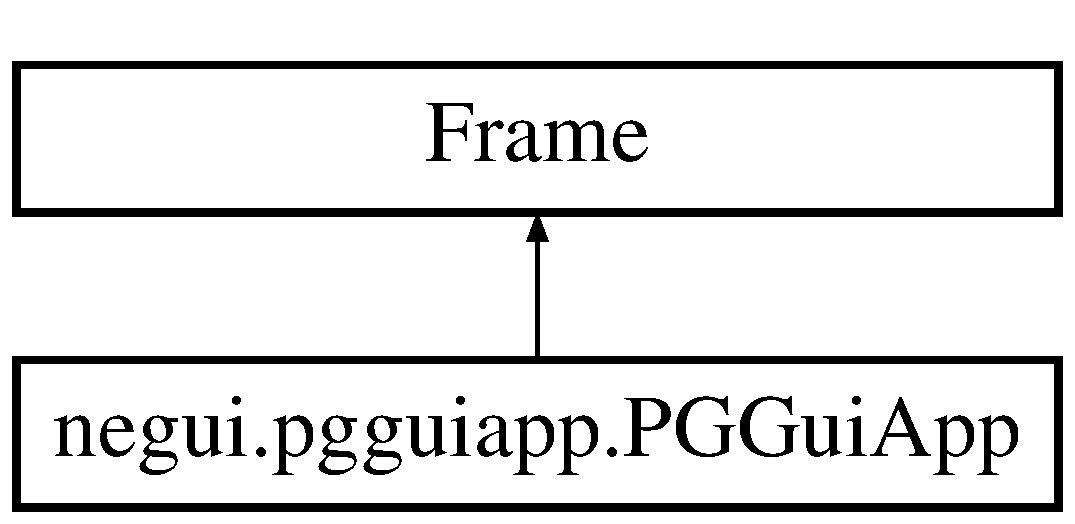
\includegraphics[height=2.000000cm]{classnegui_1_1pgguiapp_1_1PGGuiApp}
\end{center}
\end{figure}
\subsection*{Public Member Functions}
\begin{DoxyCompactItemize}
\item 
def {\bfseries \+\_\+\+\_\+init\+\_\+\+\_\+} (self, s\+\_\+name, \hyperlink{classnegui_1_1pgguiapp_1_1PGGuiApp_a0af5ea1a1b6d1565002150d7b53efbdc}{master}=None)\hypertarget{classnegui_1_1pgguiapp_1_1PGGuiApp_a0490187d0d326fa3582bb5832fc3e79c}{}\label{classnegui_1_1pgguiapp_1_1PGGuiApp_a0490187d0d326fa3582bb5832fc3e79c}

\item 
def \hyperlink{classnegui_1_1pgguiapp_1_1PGGuiApp_a0af5ea1a1b6d1565002150d7b53efbdc}{master} (self)
\item 
def \hyperlink{classnegui_1_1pgguiapp_1_1PGGuiApp_a9721978e605adde6c1bbcc8e243705fc}{master} (self, v\+\_\+value)
\item 
def {\bfseries master} (self)\hypertarget{classnegui_1_1pgguiapp_1_1PGGuiApp_a0af5ea1a1b6d1565002150d7b53efbdc}{}\label{classnegui_1_1pgguiapp_1_1PGGuiApp_a0af5ea1a1b6d1565002150d7b53efbdc}

\end{DoxyCompactItemize}


\subsection{Detailed Description}
\begin{DoxyVerb}The standard way to deploy tkinter with application object that inherits Frame
(see example at https://docs.python.org/2/library/tkinter.html#Tkinter.Tk)
this app instantiated by driver code like, 

root = Tk()
app = Application(master=root)
app.mainloop()
root.destroy()

Adds member attribute "master" (ref to the master Tk() object).
This class is to be subclassed by specific PGGui* classes that
perform specific PG operations (ex: class PGGuiSimuPop).
\end{DoxyVerb}
 

Definition at line 15 of file pgguiapp.\+py.



\subsection{Member Function Documentation}
\index{negui\+::pgguiapp\+::\+P\+G\+Gui\+App@{negui\+::pgguiapp\+::\+P\+G\+Gui\+App}!master@{master}}
\index{master@{master}!negui\+::pgguiapp\+::\+P\+G\+Gui\+App@{negui\+::pgguiapp\+::\+P\+G\+Gui\+App}}
\subsubsection[{\texorpdfstring{master(self)}{master(self)}}]{\setlength{\rightskip}{0pt plus 5cm}def negui.\+pgguiapp.\+P\+G\+Gui\+App.\+master (
\begin{DoxyParamCaption}
\item[{}]{self}
\end{DoxyParamCaption}
)}\hypertarget{classnegui_1_1pgguiapp_1_1PGGuiApp_a0af5ea1a1b6d1565002150d7b53efbdc}{}\label{classnegui_1_1pgguiapp_1_1PGGuiApp_a0af5ea1a1b6d1565002150d7b53efbdc}
\begin{DoxyVerb}master, tk.TK() object\end{DoxyVerb}
 

Definition at line 38 of file pgguiapp.\+py.


\begin{DoxyCode}
38     \textcolor{keyword}{def }\hyperlink{classnegui_1_1pgguiapp_1_1PGGuiApp_a0af5ea1a1b6d1565002150d7b53efbdc}{master}(self):
39         \textcolor{stringliteral}{"""master, tk.TK() object"""}
40         \textcolor{keywordflow}{return} self.\hyperlink{classnegui_1_1pgguiapp_1_1PGGuiApp_a2c0bf5603d97681a9cce6b2df7cd3bd3}{\_\_master}
\end{DoxyCode}
\index{negui\+::pgguiapp\+::\+P\+G\+Gui\+App@{negui\+::pgguiapp\+::\+P\+G\+Gui\+App}!master@{master}}
\index{master@{master}!negui\+::pgguiapp\+::\+P\+G\+Gui\+App@{negui\+::pgguiapp\+::\+P\+G\+Gui\+App}}
\subsubsection[{\texorpdfstring{master(self, v\+\_\+value)}{master(self, v_value)}}]{\setlength{\rightskip}{0pt plus 5cm}def negui.\+pgguiapp.\+P\+G\+Gui\+App.\+master (
\begin{DoxyParamCaption}
\item[{}]{self, }
\item[{}]{v\+\_\+value}
\end{DoxyParamCaption}
)}\hypertarget{classnegui_1_1pgguiapp_1_1PGGuiApp_a9721978e605adde6c1bbcc8e243705fc}{}\label{classnegui_1_1pgguiapp_1_1PGGuiApp_a9721978e605adde6c1bbcc8e243705fc}
\begin{DoxyVerb}raise Exception( "in PGGuiApp object, " \
+ "there is no setter for the master object. " )
\end{DoxyVerb}
 

Definition at line 44 of file pgguiapp.\+py.


\begin{DoxyCode}
44     \textcolor{keyword}{def }\hyperlink{classnegui_1_1pgguiapp_1_1PGGuiApp_a0af5ea1a1b6d1565002150d7b53efbdc}{master}( self, v\_value ):
45         \textcolor{stringliteral}{'''}
46 \textcolor{stringliteral}{        raise Exception( "in PGGuiApp object, " \(\backslash\)}
47 \textcolor{stringliteral}{        + "there is no setter for the master object. " )}
48 \textcolor{stringliteral}{        '''}
49         self.\hyperlink{classnegui_1_1pgguiapp_1_1PGGuiApp_a2c0bf5603d97681a9cce6b2df7cd3bd3}{\_\_master} = v\_value
50         \textcolor{keywordflow}{return}
\end{DoxyCode}


The documentation for this class was generated from the following file\+:\begin{DoxyCompactItemize}
\item 
pgguiapp.\+py\end{DoxyCompactItemize}

\hypertarget{classnegui_1_1pgguiutilities_1_1PGGUIErrorMessage}{}\section{negui.\+pgguiutilities.\+P\+G\+G\+U\+I\+Error\+Message Class Reference}
\label{classnegui_1_1pgguiutilities_1_1PGGUIErrorMessage}\index{negui.\+pgguiutilities.\+P\+G\+G\+U\+I\+Error\+Message@{negui.\+pgguiutilities.\+P\+G\+G\+U\+I\+Error\+Message}}
Inheritance diagram for negui.\+pgguiutilities.\+P\+G\+G\+U\+I\+Error\+Message\+:\begin{figure}[H]
\begin{center}
\leavevmode
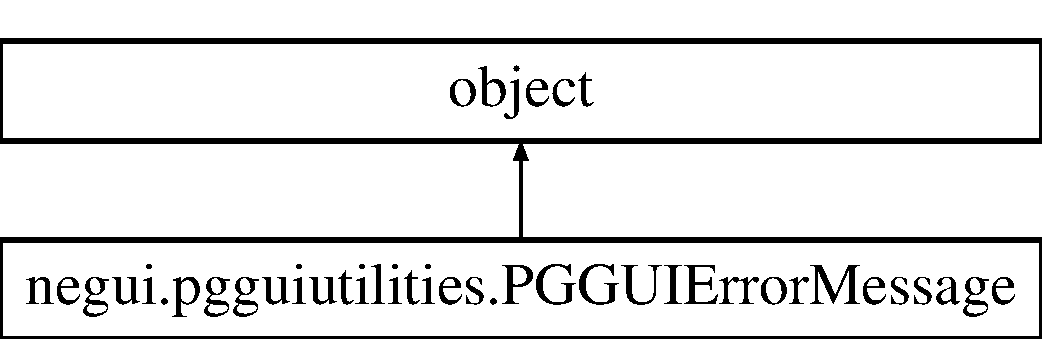
\includegraphics[height=2.000000cm]{classnegui_1_1pgguiutilities_1_1PGGUIErrorMessage}
\end{center}
\end{figure}
\subsection*{Public Member Functions}
\begin{DoxyCompactItemize}
\item 
def {\bfseries \+\_\+\+\_\+init\+\_\+\+\_\+} (self, o\+\_\+parent, s\+\_\+message)\hypertarget{classnegui_1_1pgguiutilities_1_1PGGUIErrorMessage_a420fb489448327d2a25e10f35a6c3589}{}\label{classnegui_1_1pgguiutilities_1_1PGGUIErrorMessage_a420fb489448327d2a25e10f35a6c3589}

\end{DoxyCompactItemize}


\subsection{Detailed Description}


Definition at line 962 of file pgguiutilities.\+py.



The documentation for this class was generated from the following file\+:\begin{DoxyCompactItemize}
\item 
pgguiutilities.\+py\end{DoxyCompactItemize}

\hypertarget{classnegui_1_1pgguiutilities_1_1PGGUIInfoMessage}{}\section{negui.\+pgguiutilities.\+P\+G\+G\+U\+I\+Info\+Message Class Reference}
\label{classnegui_1_1pgguiutilities_1_1PGGUIInfoMessage}\index{negui.\+pgguiutilities.\+P\+G\+G\+U\+I\+Info\+Message@{negui.\+pgguiutilities.\+P\+G\+G\+U\+I\+Info\+Message}}
Inheritance diagram for negui.\+pgguiutilities.\+P\+G\+G\+U\+I\+Info\+Message\+:\begin{figure}[H]
\begin{center}
\leavevmode
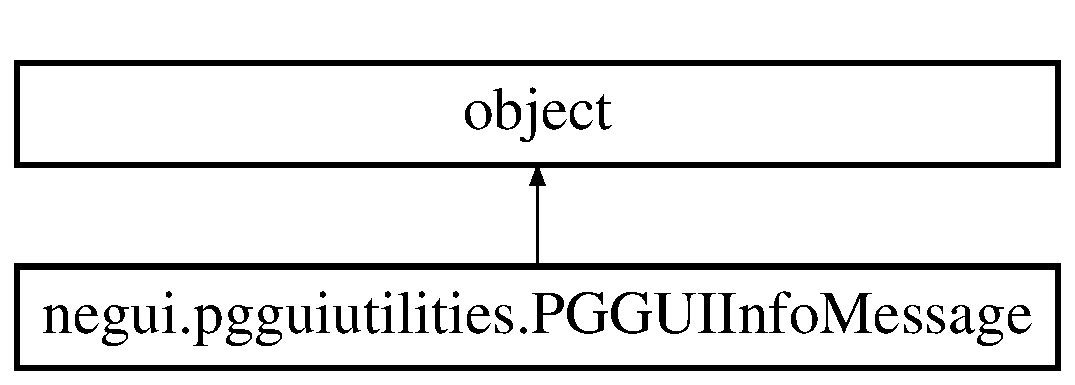
\includegraphics[height=2.000000cm]{classnegui_1_1pgguiutilities_1_1PGGUIInfoMessage}
\end{center}
\end{figure}
\subsection*{Public Member Functions}
\begin{DoxyCompactItemize}
\item 
def {\bfseries \+\_\+\+\_\+init\+\_\+\+\_\+} (self, o\+\_\+parent, s\+\_\+message)\hypertarget{classnegui_1_1pgguiutilities_1_1PGGUIInfoMessage_a6610dd669862924d49f1ec400b4df128}{}\label{classnegui_1_1pgguiutilities_1_1PGGUIInfoMessage_a6610dd669862924d49f1ec400b4df128}

\end{DoxyCompactItemize}


\subsection{Detailed Description}


Definition at line 1374 of file pgguiutilities.\+py.



The documentation for this class was generated from the following file\+:\begin{DoxyCompactItemize}
\item 
pgguiutilities.\+py\end{DoxyCompactItemize}

\hypertarget{classnegui_1_1pgguiutilities_1_1PGGUIMessageAndActionOnCancel}{}\section{negui.\+pgguiutilities.\+P\+G\+G\+U\+I\+Message\+And\+Action\+On\+Cancel Class Reference}
\label{classnegui_1_1pgguiutilities_1_1PGGUIMessageAndActionOnCancel}\index{negui.\+pgguiutilities.\+P\+G\+G\+U\+I\+Message\+And\+Action\+On\+Cancel@{negui.\+pgguiutilities.\+P\+G\+G\+U\+I\+Message\+And\+Action\+On\+Cancel}}
Inheritance diagram for negui.\+pgguiutilities.\+P\+G\+G\+U\+I\+Message\+And\+Action\+On\+Cancel\+:\begin{figure}[H]
\begin{center}
\leavevmode
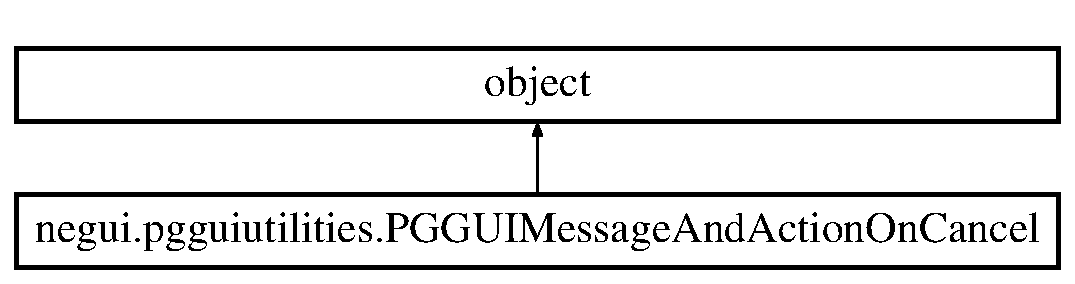
\includegraphics[height=2.000000cm]{classnegui_1_1pgguiutilities_1_1PGGUIMessageAndActionOnCancel}
\end{center}
\end{figure}
\subsection*{Public Member Functions}
\begin{DoxyCompactItemize}
\item 
def {\bfseries \+\_\+\+\_\+init\+\_\+\+\_\+} (self, o\+\_\+parent, s\+\_\+message, def\+\_\+on\+\_\+cancel)\hypertarget{classnegui_1_1pgguiutilities_1_1PGGUIMessageAndActionOnCancel_a4274202cb2f6a6ef64a3928c9d433aff}{}\label{classnegui_1_1pgguiutilities_1_1PGGUIMessageAndActionOnCancel_a4274202cb2f6a6ef64a3928c9d433aff}

\end{DoxyCompactItemize}


\subsection{Detailed Description}


Definition at line 983 of file pgguiutilities.\+py.



The documentation for this class was generated from the following file\+:\begin{DoxyCompactItemize}
\item 
pgguiutilities.\+py\end{DoxyCompactItemize}

\hypertarget{classnegui_1_1pgguisimupop_1_1PGGuiSimuPop}{}\section{negui.\+pgguisimupop.\+P\+G\+Gui\+Simu\+Pop Class Reference}
\label{classnegui_1_1pgguisimupop_1_1PGGuiSimuPop}\index{negui.\+pgguisimupop.\+P\+G\+Gui\+Simu\+Pop@{negui.\+pgguisimupop.\+P\+G\+Gui\+Simu\+Pop}}
Inheritance diagram for negui.\+pgguisimupop.\+P\+G\+Gui\+Simu\+Pop\+:\begin{figure}[H]
\begin{center}
\leavevmode
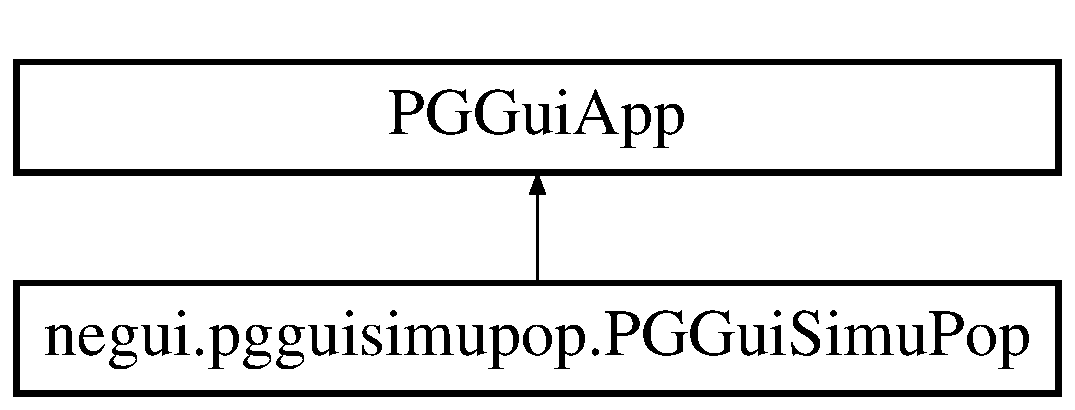
\includegraphics[height=2.000000cm]{classnegui_1_1pgguisimupop_1_1PGGuiSimuPop}
\end{center}
\end{figure}
\subsection*{Public Member Functions}
\begin{DoxyCompactItemize}
\item 
def \hyperlink{classnegui_1_1pgguisimupop_1_1PGGuiSimuPop_aa159ead5d8fbd28d693c9021db12b95e}{\+\_\+\+\_\+init\+\_\+\+\_\+} (self, o\+\_\+parent, s\+\_\+param\+\_\+names\+\_\+file=None, s\+\_\+life\+\_\+table\+\_\+file\+\_\+glob=\char`\"{}resources/$\ast$life.\+table.\+info\char`\"{}, s\+\_\+name=\char`\"{}simupop\+\_\+gui\char`\"{}, i\+\_\+total\+\_\+processes\+\_\+for\+\_\+sims=1)
\item 
def \hyperlink{classnegui_1_1pgguisimupop_1_1PGGuiSimuPop_ad1d590f23bbaf0eda730d488ea74c1ba}{on\+Cull\+Method\+Selection\+Change} (self)
\item 
def {\bfseries load\+\_\+config\+\_\+file} (self, event=None)\hypertarget{classnegui_1_1pgguisimupop_1_1PGGuiSimuPop_a9ae755614518ece6584d83aff129f4d5}{}\label{classnegui_1_1pgguisimupop_1_1PGGuiSimuPop_a9ae755614518ece6584d83aff129f4d5}

\item 
def \hyperlink{classnegui_1_1pgguisimupop_1_1PGGuiSimuPop_ac193cf44f5e4f1e5b146a43e9563d7b0}{update\+N0\+Entry\+Box} (self)
\item 
def {\bfseries select\+\_\+output\+\_\+directory} (self, event=None)\hypertarget{classnegui_1_1pgguisimupop_1_1PGGuiSimuPop_a4d88e502ff12249698177dbb4336715d}{}\label{classnegui_1_1pgguisimupop_1_1PGGuiSimuPop_a4d88e502ff12249698177dbb4336715d}

\item 
def {\bfseries run\+Simulation} (self)\hypertarget{classnegui_1_1pgguisimupop_1_1PGGuiSimuPop_a7dc99019295f2a2650fa95ecddd55239}{}\label{classnegui_1_1pgguisimupop_1_1PGGuiSimuPop_a7dc99019295f2a2650fa95ecddd55239}

\item 
def {\bfseries cleanup} (self)\hypertarget{classnegui_1_1pgguisimupop_1_1PGGuiSimuPop_a24642a8bffa19a61a4fb1b6d5e9f0a1c}{}\label{classnegui_1_1pgguisimupop_1_1PGGuiSimuPop_a24642a8bffa19a61a4fb1b6d5e9f0a1c}

\end{DoxyCompactItemize}
\subsection*{Public Attributes}
\begin{DoxyCompactItemize}
\item 
{\bfseries output\+\_\+base\+\_\+name}\hypertarget{classnegui_1_1pgguisimupop_1_1PGGuiSimuPop_aa5f9f17f0527c20e5556b574a3f97300}{}\label{classnegui_1_1pgguisimupop_1_1PGGuiSimuPop_aa5f9f17f0527c20e5556b574a3f97300}

\end{DoxyCompactItemize}
\subsection*{Static Public Attributes}
\begin{DoxyCompactItemize}
\item 
int {\bfseries R\+U\+N\+\_\+\+N\+O\+T\+\_\+\+R\+E\+A\+DY} = 0\hypertarget{classnegui_1_1pgguisimupop_1_1PGGuiSimuPop_ae82d4be656ee869a30087fe2bab1410e}{}\label{classnegui_1_1pgguisimupop_1_1PGGuiSimuPop_ae82d4be656ee869a30087fe2bab1410e}

\item 
int {\bfseries R\+U\+N\+\_\+\+R\+E\+A\+DY} = 1\hypertarget{classnegui_1_1pgguisimupop_1_1PGGuiSimuPop_ab29a3c49b505f46c6a648dce7772fa80}{}\label{classnegui_1_1pgguisimupop_1_1PGGuiSimuPop_ab29a3c49b505f46c6a648dce7772fa80}

\item 
int {\bfseries R\+U\+N\+\_\+\+I\+N\+\_\+\+P\+R\+O\+G\+R\+E\+SS} = 2\hypertarget{classnegui_1_1pgguisimupop_1_1PGGuiSimuPop_a023efccec69461c3f9898383c24bb24b}{}\label{classnegui_1_1pgguisimupop_1_1PGGuiSimuPop_a023efccec69461c3f9898383c24bb24b}

\item 
int {\bfseries M\+A\+X\+\_\+\+C\+H\+A\+R\+S\+\_\+\+B\+A\+S\+E\+N\+A\+ME} = 18\hypertarget{classnegui_1_1pgguisimupop_1_1PGGuiSimuPop_a75a723ea82c8855efce337740a1e4c91}{}\label{classnegui_1_1pgguisimupop_1_1PGGuiSimuPop_a75a723ea82c8855efce337740a1e4c91}

\end{DoxyCompactItemize}


\subsection{Detailed Description}
\begin{DoxyVerb}Subclass of PGGuiApp builds a gui,
creates PGInputSimuPop and PGOutputSimuPop
objects, then on user command runs a simulation 
(one or more replicates) based on the parameters 
supplied by the Input object, and to output files 
as named by the basename in the PGOutputSimuPop object.  

Note that for this class I abandoned my intended original 
organization of the functionality for all  PGGuiApp objects.
All subclasses of PGGUIApp objects were to contain an 
AGPOperation object, in this case aPGOpSimuPop object, 
which contains the code that actually uses Tiago Antao's 
code to setup and run a SimuPOP session.  However, in 
implenting replicate runs I encountered errors when
trying to target a class method when spawning python
multiprocessing.process objects from this object.  Further,
I found non-independant instantiation of simupop populations 
even when instantiating new PGOpSimuPop objects constructed
in separate python multiprocessing.process instances.   
Thus, parallel processing of simulation replicates required 
the use of separate python instances for each replicate. 
Thus currently (Wed Jul 27 18:35:05 MDT 2016),
instead of manipulating its own PGOpSimuPop instances,
this class depends on code in the pgutilities.py
module, which has a def that makes a system call to 
instantiate a new python interpreter, and call a script,
do_sim_replicate.py, which then calls another def in 
pgutilities.py, which builds and runs a PGOpSimuPop object.\end{DoxyVerb}
 

Definition at line 60 of file pgguisimupop.\+py.



\subsection{Constructor \& Destructor Documentation}
\index{negui\+::pgguisimupop\+::\+P\+G\+Gui\+Simu\+Pop@{negui\+::pgguisimupop\+::\+P\+G\+Gui\+Simu\+Pop}!\+\_\+\+\_\+init\+\_\+\+\_\+@{\+\_\+\+\_\+init\+\_\+\+\_\+}}
\index{\+\_\+\+\_\+init\+\_\+\+\_\+@{\+\_\+\+\_\+init\+\_\+\+\_\+}!negui\+::pgguisimupop\+::\+P\+G\+Gui\+Simu\+Pop@{negui\+::pgguisimupop\+::\+P\+G\+Gui\+Simu\+Pop}}
\subsubsection[{\texorpdfstring{\+\_\+\+\_\+init\+\_\+\+\_\+(self, o\+\_\+parent, s\+\_\+param\+\_\+names\+\_\+file=\+None, s\+\_\+life\+\_\+table\+\_\+file\+\_\+glob=""resources/$\ast$life.\+table.\+info"", s\+\_\+name=""simupop\+\_\+gui"", i\+\_\+total\+\_\+processes\+\_\+for\+\_\+sims=1)}{__init__(self, o_parent, s_param_names_file=None, s_life_table_file_glob="resources/*life.table.info", s_name="simupop_gui", i_total_processes_for_sims=1)}}]{\setlength{\rightskip}{0pt plus 5cm}def negui.\+pgguisimupop.\+P\+G\+Gui\+Simu\+Pop.\+\_\+\+\_\+init\+\_\+\+\_\+ (
\begin{DoxyParamCaption}
\item[{}]{self, }
\item[{}]{o\+\_\+parent, }
\item[{}]{s\+\_\+param\+\_\+names\+\_\+file = {\ttfamily None}, }
\item[{}]{s\+\_\+life\+\_\+table\+\_\+file\+\_\+glob = {\ttfamily \char`\"{}resources/$\ast$life.table.info\char`\"{}}, }
\item[{}]{s\+\_\+name = {\ttfamily \char`\"{}simupop\+\_\+gui\char`\"{}}, }
\item[{}]{i\+\_\+total\+\_\+processes\+\_\+for\+\_\+sims = {\ttfamily 1}}
\end{DoxyParamCaption}
)}\hypertarget{classnegui_1_1pgguisimupop_1_1PGGuiSimuPop_aa159ead5d8fbd28d693c9021db12b95e}{}\label{classnegui_1_1pgguisimupop_1_1PGGuiSimuPop_aa159ead5d8fbd28d693c9021db12b95e}
\begin{DoxyVerb}param s_param_names_file is the file that contains short and long param
names, used to make the PGParamSet object  member of the PGInputSimuPop 
object
\end{DoxyVerb}
 

Definition at line 104 of file pgguisimupop.\+py.


\begin{DoxyCode}
104                             i\_total\_processes\_for\_sims=1 ):
105         \textcolor{stringliteral}{'''}
106 \textcolor{stringliteral}{        param s\_param\_names\_file is the file that contains short and long param}
107 \textcolor{stringliteral}{        names, used to make the PGParamSet object  member of the PGInputSimuPop }
108 \textcolor{stringliteral}{        object}
109 \textcolor{stringliteral}{        '''}
110 
111         \textcolor{comment}{#note this call to super does not work -- a look as stackoverflow}
112         \textcolor{comment}{#chatter about this indicates that because PGGUIApp inherits Frame,}
113         \textcolor{comment}{#that Frame must be an "old-style" class (does not inherit from "object")}
114         \textcolor{comment}{#--rem out super( PGGuiSimuPop, self ).\_\_init\_\_( o\_parent )}
115         \textcolor{comment}{#instead of call to "super":}
116         pgg.PGGuiApp.\_\_init\_\_( self, s\_name, o\_parent )
117         self.\hyperlink{classnegui_1_1pgguisimupop_1_1PGGuiSimuPop_accf4b1e619efda180dcd4795425f88c8}{\_\_config\_file}=StringVar()
118         self.\hyperlink{classnegui_1_1pgguisimupop_1_1PGGuiSimuPop_a8c3dba3a47984c6174e659458da1d4c6}{\_\_output\_directory}=StringVar()
119         self.\hyperlink{classnegui_1_1pgguisimupop_1_1PGGuiSimuPop_a1871547ce6fe9a86b10a30f3d7b41cdd}{\_\_life\_table\_files}=[]
120         self.\hyperlink{classnegui_1_1pgguisimupop_1_1PGGuiSimuPop_a12344f4fdce230b8fbb699dbd74c95a2}{\_\_get\_life\_table\_file\_list}( s\_life\_table\_file\_glob )
121 
122         \textcolor{comment}{#we use the tkinter traceable variable}
123         \textcolor{comment}{#so that, when loaded into an entry box}
124         \textcolor{comment}{#we can auto update the value as it is }
125         \textcolor{comment}{#user-edited:}
126         self.\_\_output\_directory.set( self.\hyperlink{classnegui_1_1pgguisimupop_1_1PGGuiSimuPop_abba3f28989d693eadf8d8dd181502d06}{\_\_get\_default\_output\_directory}() )
127 
128         self.\hyperlink{classnegui_1_1pgguisimupop_1_1PGGuiSimuPop_aa5f9f17f0527c20e5556b574a3f97300}{output\_base\_name}=self.
      \hyperlink{classnegui_1_1pgguisimupop_1_1PGGuiSimuPop_a55130312327d03aa8e37d827a46929db}{\_\_get\_default\_output\_base\_name}() 
129 
130         \textcolor{comment}{#the PGOpSimuPop object:}
131         self.\hyperlink{classnegui_1_1pgguisimupop_1_1PGGuiSimuPop_a53d091be0140a85e8c45a76c0b89c370}{\_\_param\_names\_file}=s\_param\_names\_file
132 
133         \textcolor{comment}{#input object used to make the}
134         \textcolor{comment}{#operation object type PGOpSimuPop}
135         self.\hyperlink{classnegui_1_1pgguisimupop_1_1PGGuiSimuPop_a0b9f7d933b428393d34105828600a007}{\_\_input}=\textcolor{keywordtype}{None}
136         \textcolor{comment}{#output object used to}
137         \textcolor{comment}{#name and create the simulation}
138         \textcolor{comment}{#output files}
139         self.\hyperlink{classnegui_1_1pgguisimupop_1_1PGGuiSimuPop_a30f6eabf78230001520f90cb36de339f}{\_\_output}=\textcolor{keywordtype}{None}
140 
141         \textcolor{comment}{#when commanded to run the simulation(s)}
142         \textcolor{comment}{#a temporary configuration file}
143         \textcolor{comment}{#is created and used by each process}
144         \textcolor{comment}{#that is simulating.  We then want to}
145         \textcolor{comment}{#delete the file when the gui had }
146         \textcolor{comment}{#ascertained that the sim is or sims}
147         \textcolor{comment}{#are done, so we need instance-level}
148         \textcolor{comment}{#access to the file name}
149         self.\hyperlink{classnegui_1_1pgguisimupop_1_1PGGuiSimuPop_a60c4be477f462c6981a08c479c20a893}{\_\_temp\_config\_file\_for\_running\_replicates}=\textcolor{keywordtype}{None}
150 
151         \textcolor{comment}{#simulations performed on separate}
152         \textcolor{comment}{#process -- this ref to it will}
153         \textcolor{comment}{#enable checking whether in progress}
154         \textcolor{comment}{#or finished.  See def runSimulation:}
155         self.\hyperlink{classnegui_1_1pgguisimupop_1_1PGGuiSimuPop_acdcfde3516741c64806c6881f65c6f4e}{\_\_op\_process}=\textcolor{keywordtype}{None}
156         \textcolor{comment}{#we set this before spawning \_\_op\_process,}
157         \textcolor{comment}{#so that on cancel-sim, we can}
158         \textcolor{comment}{#notify op\_process and it can }
159         \textcolor{comment}{#clean up its subprocesses and }
160         \textcolor{comment}{#output:}
161         self.\hyperlink{classnegui_1_1pgguisimupop_1_1PGGuiSimuPop_a02ccc7da9aec67e8e13e083001aba15b}{\_\_sim\_multi\_process\_event}=\textcolor{keywordtype}{None}
162 
163         \textcolor{comment}{#we have a default output name,}
164         \textcolor{comment}{#so we can init the output}
165         \textcolor{comment}{#immediately}
166         self.\hyperlink{classnegui_1_1pgguisimupop_1_1PGGuiSimuPop_a23913431472d154054d66ab5e72daf0e}{\_\_setup\_output}()
167 
168 
169 
170         self.\hyperlink{classnegui_1_1pgguisimupop_1_1PGGuiSimuPop_a5064bac64c69bd13fe1366b21f1f7ad9}{\_\_simulation\_is\_in\_progress}=\textcolor{keyword}{False}
171 
172         self.\hyperlink{classnegui_1_1pgguisimupop_1_1PGGuiSimuPop_a3885325060336297119229764f6548fb}{\_\_total\_processes\_for\_sims}=i\_total\_processes\_for\_sims
173 
174         \textcolor{comment}{#we hold references to all subframes}
175         \textcolor{comment}{#except the run-button subframe,}
176         \textcolor{comment}{#so that we can enable/disable}
177         \textcolor{comment}{#according to the simulation-run state}
178         \textcolor{comment}{#(not yet implemented, 2016\_08\_05}
179 
180         self.\hyperlink{classnegui_1_1pgguisimupop_1_1PGGuiSimuPop_a67da63f36462b56bd1f47206d8f91c7b}{\_\_category\_frames}=\textcolor{keywordtype}{None}
181 
182         \textcolor{comment}{#we also hold refernces to the keyvalue}
183         \textcolor{comment}{#frames that hold param values.  This}
184         \textcolor{comment}{#allows us to communicate with the entry}
185         \textcolor{comment}{#boxes via param name.}
186         self.\hyperlink{classnegui_1_1pgguisimupop_1_1PGGuiSimuPop_a272523ce4bad4d1073c506e858c59996}{\_\_param\_key\_value\_frames}=\textcolor{keywordtype}{None}
187 
188 
189         self.\hyperlink{classnegui_1_1pgguisimupop_1_1PGGuiSimuPop_a3ac3a7a5a800876180133b4cc41ca63c}{\_\_run\_state\_message}=\textcolor{stringliteral}{""}
190         self.\hyperlink{classnegui_1_1pgguisimupop_1_1PGGuiSimuPop_ad38b601eabe45f6c35525b060f0343ea}{\_\_init\_interface}()
191         self.\hyperlink{classnegui_1_1pgguisimupop_1_1PGGuiSimuPop_a2c5268e62f40c2548d1475959aa60ca9}{\_\_set\_controls\_by\_run\_state}( self.
      \hyperlink{classnegui_1_1pgguisimupop_1_1PGGuiSimuPop_aef182e14bccdbabf372a6344bc6f8786}{\_\_get\_run\_state}() )
192     
193         \textcolor{keywordflow}{return}
\end{DoxyCode}


\subsection{Member Function Documentation}
\index{negui\+::pgguisimupop\+::\+P\+G\+Gui\+Simu\+Pop@{negui\+::pgguisimupop\+::\+P\+G\+Gui\+Simu\+Pop}!on\+Cull\+Method\+Selection\+Change@{on\+Cull\+Method\+Selection\+Change}}
\index{on\+Cull\+Method\+Selection\+Change@{on\+Cull\+Method\+Selection\+Change}!negui\+::pgguisimupop\+::\+P\+G\+Gui\+Simu\+Pop@{negui\+::pgguisimupop\+::\+P\+G\+Gui\+Simu\+Pop}}
\subsubsection[{\texorpdfstring{on\+Cull\+Method\+Selection\+Change(self)}{onCullMethodSelectionChange(self)}}]{\setlength{\rightskip}{0pt plus 5cm}def negui.\+pgguisimupop.\+P\+G\+Gui\+Simu\+Pop.\+on\+Cull\+Method\+Selection\+Change (
\begin{DoxyParamCaption}
\item[{}]{self}
\end{DoxyParamCaption}
)}\hypertarget{classnegui_1_1pgguisimupop_1_1PGGuiSimuPop_ad1d590f23bbaf0eda730d488ea74c1ba}{}\label{classnegui_1_1pgguisimupop_1_1PGGuiSimuPop_ad1d590f23bbaf0eda730d488ea74c1ba}
\begin{DoxyVerb}Not implemented, 2016_11_01.  May
not need to add any code here, since
KeyListComboFrame control object resets
the attribute in the input object
automatically.
\end{DoxyVerb}
 

Definition at line 718 of file pgguisimupop.\+py.


\begin{DoxyCode}
718     \textcolor{keyword}{def }\hyperlink{classnegui_1_1pgguisimupop_1_1PGGuiSimuPop_ad1d590f23bbaf0eda730d488ea74c1ba}{onCullMethodSelectionChange}( self ):
719         \textcolor{stringliteral}{'''}
720 \textcolor{stringliteral}{        Not implemented, 2016\_11\_01.  May}
721 \textcolor{stringliteral}{        not need to add any code here, since}
722 \textcolor{stringliteral}{        KeyListComboFrame control object resets}
723 \textcolor{stringliteral}{        the attribute in the input object}
724 \textcolor{stringliteral}{        automatically.}
725 \textcolor{stringliteral}{        '''}
726 
727         \textcolor{keywordflow}{if} VERY\_VERBOSE:
728             self.\hyperlink{classnegui_1_1pgguisimupop_1_1PGGuiSimuPop_a1a916d4c19afe08b2c7772d099c71f3f}{\_\_test\_value}()
729         \textcolor{comment}{#end if very verbose}
730 
731         \textcolor{keywordflow}{return}
\end{DoxyCode}
\index{negui\+::pgguisimupop\+::\+P\+G\+Gui\+Simu\+Pop@{negui\+::pgguisimupop\+::\+P\+G\+Gui\+Simu\+Pop}!update\+N0\+Entry\+Box@{update\+N0\+Entry\+Box}}
\index{update\+N0\+Entry\+Box@{update\+N0\+Entry\+Box}!negui\+::pgguisimupop\+::\+P\+G\+Gui\+Simu\+Pop@{negui\+::pgguisimupop\+::\+P\+G\+Gui\+Simu\+Pop}}
\subsubsection[{\texorpdfstring{update\+N0\+Entry\+Box(self)}{updateN0EntryBox(self)}}]{\setlength{\rightskip}{0pt plus 5cm}def negui.\+pgguisimupop.\+P\+G\+Gui\+Simu\+Pop.\+update\+N0\+Entry\+Box (
\begin{DoxyParamCaption}
\item[{}]{self}
\end{DoxyParamCaption}
)}\hypertarget{classnegui_1_1pgguisimupop_1_1PGGuiSimuPop_ac193cf44f5e4f1e5b146a43e9563d7b0}{}\label{classnegui_1_1pgguisimupop_1_1PGGuiSimuPop_ac193cf44f5e4f1e5b146a43e9563d7b0}
\begin{DoxyVerb}N0 parameter updates differently according to
whether it is simply taken from a config file's
pop section, or, alternatively, calculated from
params Nb,Nb/Nc as given by an "effective_size"
section in a life table or config file, and also
using input params maleProb, survivalMale, and
survivalFemale.  In the latter
case, the keyvalue frame will be disabled and its entrybox
will be manually updated from this def.  
\end{DoxyVerb}
 

Definition at line 762 of file pgguisimupop.\+py.


\begin{DoxyCode}
762     \textcolor{keyword}{def }\hyperlink{classnegui_1_1pgguisimupop_1_1PGGuiSimuPop_ac193cf44f5e4f1e5b146a43e9563d7b0}{updateN0EntryBox}( self ):
763         \textcolor{stringliteral}{'''}
764 \textcolor{stringliteral}{        N0 parameter updates differently according to}
765 \textcolor{stringliteral}{        whether it is simply taken from a config file's}
766 \textcolor{stringliteral}{        pop section, or, alternatively, calculated from}
767 \textcolor{stringliteral}{        params Nb,Nb/Nc as given by an "effective\_size"}
768 \textcolor{stringliteral}{        section in a life table or config file, and also}
769 \textcolor{stringliteral}{        using input params maleProb, survivalMale, and}
770 \textcolor{stringliteral}{        survivalFemale.  In the latter}
771 \textcolor{stringliteral}{        case, the keyvalue frame will be disabled and its entrybox}
772 \textcolor{stringliteral}{        will be manually updated from this def.  }
773 \textcolor{stringliteral}{        '''}
774         \textcolor{keywordflow}{if} self.\_\_input.N0IsCalculatedFromEffectiveSizeInfo():
775             \textcolor{stringliteral}{'''}
776 \textcolor{stringliteral}{            Nb is a property, calculated or just returned}
777 \textcolor{stringliteral}{            depending on its source (effec size or hus a value}
778 \textcolor{stringliteral}{            given in the pop section). The property def in}
779 \textcolor{stringliteral}{            our \_\_input member will test the state and calculate}
780 \textcolor{stringliteral}{            N0 accordingly:}
781 \textcolor{stringliteral}{            '''}
782 
783             i\_current\_n0\_val=self.\_\_input.N0
784 
785             self.\hyperlink{classnegui_1_1pgguisimupop_1_1PGGuiSimuPop_a272523ce4bad4d1073c506e858c59996}{\_\_param\_key\_value\_frames}[ \textcolor{stringliteral}{"N0"} ].manuallyUpdateValue( 
      i\_current\_n0\_val )
786         \textcolor{comment}{#end if N0 is calc'd from effective size info}
787 
788         \textcolor{keywordflow}{if} VERY\_VERBOSE:
789             self.\hyperlink{classnegui_1_1pgguisimupop_1_1PGGuiSimuPop_a1a916d4c19afe08b2c7772d099c71f3f}{\_\_test\_value}()
790         \textcolor{comment}{#end if very verbose, show param values}
791 
792         \textcolor{keywordflow}{return}
\end{DoxyCode}


The documentation for this class was generated from the following file\+:\begin{DoxyCompactItemize}
\item 
pgguisimupop.\+py\end{DoxyCompactItemize}

\hypertarget{classnegui_1_1pgguiutilities_1_1PGGUIWarningMessage}{}\section{negui.\+pgguiutilities.\+P\+G\+G\+U\+I\+Warning\+Message Class Reference}
\label{classnegui_1_1pgguiutilities_1_1PGGUIWarningMessage}\index{negui.\+pgguiutilities.\+P\+G\+G\+U\+I\+Warning\+Message@{negui.\+pgguiutilities.\+P\+G\+G\+U\+I\+Warning\+Message}}
Inheritance diagram for negui.\+pgguiutilities.\+P\+G\+G\+U\+I\+Warning\+Message\+:\begin{figure}[H]
\begin{center}
\leavevmode
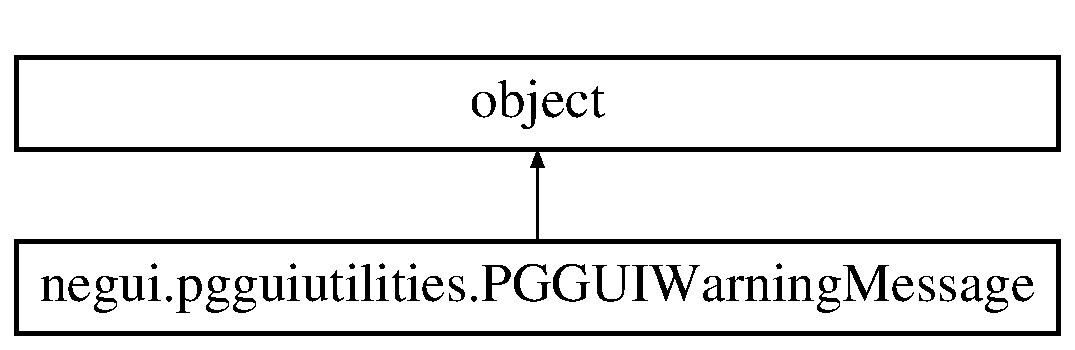
\includegraphics[height=2.000000cm]{classnegui_1_1pgguiutilities_1_1PGGUIWarningMessage}
\end{center}
\end{figure}
\subsection*{Public Member Functions}
\begin{DoxyCompactItemize}
\item 
def {\bfseries \+\_\+\+\_\+init\+\_\+\+\_\+} (self, o\+\_\+parent, s\+\_\+message)\hypertarget{classnegui_1_1pgguiutilities_1_1PGGUIWarningMessage_a0ac338d8bcaa1e19be56a0b71a222d6e}{}\label{classnegui_1_1pgguiutilities_1_1PGGUIWarningMessage_a0ac338d8bcaa1e19be56a0b71a222d6e}

\end{DoxyCompactItemize}


\subsection{Detailed Description}


Definition at line 153 of file pgguiutilities.\+py.



The documentation for this class was generated from the following file\+:\begin{DoxyCompactItemize}
\item 
pgguiutilities.\+py\end{DoxyCompactItemize}

\hypertarget{classnegui_1_1pghostnotebook_1_1PGHostNotebook}{}\section{negui.\+pghostnotebook.\+P\+G\+Host\+Notebook Class Reference}
\label{classnegui_1_1pghostnotebook_1_1PGHostNotebook}\index{negui.\+pghostnotebook.\+P\+G\+Host\+Notebook@{negui.\+pghostnotebook.\+P\+G\+Host\+Notebook}}
Inheritance diagram for negui.\+pghostnotebook.\+P\+G\+Host\+Notebook\+:\begin{figure}[H]
\begin{center}
\leavevmode
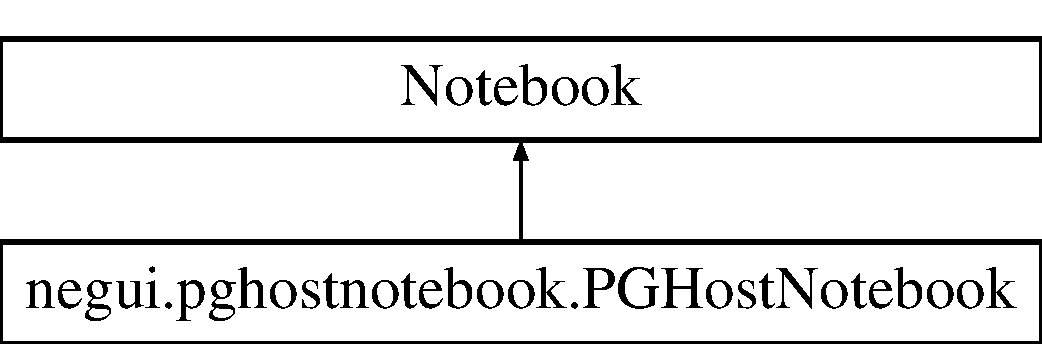
\includegraphics[height=2.000000cm]{classnegui_1_1pghostnotebook_1_1PGHostNotebook}
\end{center}
\end{figure}
\subsection*{Public Member Functions}
\begin{DoxyCompactItemize}
\item 
def \hyperlink{classnegui_1_1pghostnotebook_1_1PGHostNotebook_a6194250626f96f1f6c2b6ccd48aa5e92}{\+\_\+\+\_\+init\+\_\+\+\_\+} (self, o\+\_\+parent, s\+\_\+menu\+\_\+config, s\+\_\+param\+\_\+names\+\_\+file\+\_\+for\+\_\+simulation, s\+\_\+glob\+\_\+life\+\_\+tables=None, i\+\_\+max\+\_\+process\+\_\+total=1)
\item 
def \hyperlink{classnegui_1_1pghostnotebook_1_1PGHostNotebook_af595ed4592e623ef403a5e9e7c1e930e}{add\+P\+G\+Gui\+Simupop} (self)
\item 
def {\bfseries add\+P\+G\+Gui\+Ne\+Estimation} (self)\hypertarget{classnegui_1_1pghostnotebook_1_1PGHostNotebook_a9242f6b6eff030ac5de8db425e1585f9}{}\label{classnegui_1_1pghostnotebook_1_1PGHostNotebook_a9242f6b6eff030ac5de8db425e1585f9}

\item 
def {\bfseries exit\+Notebook} (self)\hypertarget{classnegui_1_1pghostnotebook_1_1PGHostNotebook_a6b399a4627a80141332553e637eab595}{}\label{classnegui_1_1pghostnotebook_1_1PGHostNotebook_a6b399a4627a80141332553e637eab595}

\item 
def {\bfseries remove\+Current\+Tab} (self)\hypertarget{classnegui_1_1pghostnotebook_1_1PGHostNotebook_a722efece7ca42a910310c05dd77a282b}{}\label{classnegui_1_1pghostnotebook_1_1PGHostNotebook_a722efece7ca42a910310c05dd77a282b}

\item 
def {\bfseries remove\+Tab} (self, i\+\_\+tab\+\_\+index)\hypertarget{classnegui_1_1pghostnotebook_1_1PGHostNotebook_acd199bca00bb076546ff1f2b3214cf1a}{}\label{classnegui_1_1pghostnotebook_1_1PGHostNotebook_acd199bca00bb076546ff1f2b3214cf1a}

\item 
def {\bfseries remove\+All\+Tabs} (self)\hypertarget{classnegui_1_1pghostnotebook_1_1PGHostNotebook_a1ee591325aa0128d47f46b9faf5ebf9a}{}\label{classnegui_1_1pghostnotebook_1_1PGHostNotebook_a1ee591325aa0128d47f46b9faf5ebf9a}

\end{DoxyCompactItemize}


\subsection{Detailed Description}
\begin{DoxyVerb}Interface that uses tabbed windows to implement interfaces, one or more PGGuiSimupop and/or PGGuiNeEstimator
objects.
\end{DoxyVerb}
 

Definition at line 25 of file pghostnotebook.\+py.



\subsection{Constructor \& Destructor Documentation}
\index{negui\+::pghostnotebook\+::\+P\+G\+Host\+Notebook@{negui\+::pghostnotebook\+::\+P\+G\+Host\+Notebook}!\+\_\+\+\_\+init\+\_\+\+\_\+@{\+\_\+\+\_\+init\+\_\+\+\_\+}}
\index{\+\_\+\+\_\+init\+\_\+\+\_\+@{\+\_\+\+\_\+init\+\_\+\+\_\+}!negui\+::pghostnotebook\+::\+P\+G\+Host\+Notebook@{negui\+::pghostnotebook\+::\+P\+G\+Host\+Notebook}}
\subsubsection[{\texorpdfstring{\+\_\+\+\_\+init\+\_\+\+\_\+(self, o\+\_\+parent, s\+\_\+menu\+\_\+config, s\+\_\+param\+\_\+names\+\_\+file\+\_\+for\+\_\+simulation, s\+\_\+glob\+\_\+life\+\_\+tables=\+None, i\+\_\+max\+\_\+process\+\_\+total=1)}{__init__(self, o_parent, s_menu_config, s_param_names_file_for_simulation, s_glob_life_tables=None, i_max_process_total=1)}}]{\setlength{\rightskip}{0pt plus 5cm}def negui.\+pghostnotebook.\+P\+G\+Host\+Notebook.\+\_\+\+\_\+init\+\_\+\+\_\+ (
\begin{DoxyParamCaption}
\item[{}]{self, }
\item[{}]{o\+\_\+parent, }
\item[{}]{s\+\_\+menu\+\_\+config, }
\item[{}]{s\+\_\+param\+\_\+names\+\_\+file\+\_\+for\+\_\+simulation, }
\item[{}]{s\+\_\+glob\+\_\+life\+\_\+tables = {\ttfamily None}, }
\item[{}]{i\+\_\+max\+\_\+process\+\_\+total = {\ttfamily 1}}
\end{DoxyParamCaption}
)}\hypertarget{classnegui_1_1pghostnotebook_1_1PGHostNotebook_a6194250626f96f1f6c2b6ccd48aa5e92}{}\label{classnegui_1_1pghostnotebook_1_1PGHostNotebook_a6194250626f96f1f6c2b6ccd48aa5e92}
\begin{DoxyVerb}params 
o_parent, parent ttk.Frame object

s_menu_config, file for PGMenuBuilder object, gives the main menu

s_param_names_file_for_simulation, table file that lists the parameter names
   as read into a PGInputSimuPop object

s_glob_life_tables, glob expression used by PGOpSimuPop objects to load all life tables
    into memory\end{DoxyVerb}
 

Definition at line 30 of file pghostnotebook.\+py.


\begin{DoxyCode}
30     \textcolor{keyword}{def }\hyperlink{classnegui_1_1pghostnotebook_1_1PGHostNotebook_a6194250626f96f1f6c2b6ccd48aa5e92}{\_\_init\_\_}( self, o\_parent, s\_menu\_config, s\_param\_names\_file\_for\_simulation, 
      s\_glob\_life\_tables=None, i\_max\_process\_total=1 ):
31         \textcolor{stringliteral}{'''}
32 \textcolor{stringliteral}{        params }
33 \textcolor{stringliteral}{        o\_parent, parent ttk.Frame object}
34 \textcolor{stringliteral}{}
35 \textcolor{stringliteral}{        s\_menu\_config, file for PGMenuBuilder object, gives the main menu}
36 \textcolor{stringliteral}{}
37 \textcolor{stringliteral}{        s\_param\_names\_file\_for\_simulation, table file that lists the parameter names}
38 \textcolor{stringliteral}{           as read into a PGInputSimuPop object}
39 \textcolor{stringliteral}{}
40 \textcolor{stringliteral}{        s\_glob\_life\_tables, glob expression used by PGOpSimuPop objects to load all life tables}
41 \textcolor{stringliteral}{            into memory}
42 \textcolor{stringliteral}{}
43 \textcolor{stringliteral}{        '''}
44         Notebook.\_\_init\_\_( self, o\_parent )
45         self.\hyperlink{classnegui_1_1pghostnotebook_1_1PGHostNotebook_ae3a4078b5e41c208da268dfee99bb622}{\_\_parent}=o\_parent
46         self.\hyperlink{classnegui_1_1pghostnotebook_1_1PGHostNotebook_add1ab1bb7f792ff733e8236fed00218c}{\_\_menu}=pgmb.PGMenuBuilder( s\_menu\_config, self, o\_parent )
47         self.\hyperlink{classnegui_1_1pghostnotebook_1_1PGHostNotebook_a9b145ef56ff954c480d856859fcda86e}{\_\_param\_names\_file\_for\_simulations}=
      s\_param\_names\_file\_for\_simulation
48         self.\hyperlink{classnegui_1_1pghostnotebook_1_1PGHostNotebook_a84a7417cc57500cbe5c230449ba464b3}{\_\_tab\_count}=0
49         self.\hyperlink{classnegui_1_1pghostnotebook_1_1PGHostNotebook_aa3a7876014bd06be174732b7d814bfa8}{\_\_tab\_children}=[]
50         self.\hyperlink{classnegui_1_1pghostnotebook_1_1PGHostNotebook_af63d9ae9cde1ec2155d4dc81934d00c7}{\_\_glob\_life\_tables}=s\_glob\_life\_tables
51         self.\hyperlink{classnegui_1_1pghostnotebook_1_1PGHostNotebook_a14287e3e1cf5c33d9be0ff28d031fc04}{\_\_max\_process\_total}=i\_max\_process\_total
52 
53         \textcolor{keywordflow}{return}
\end{DoxyCode}


\subsection{Member Function Documentation}
\index{negui\+::pghostnotebook\+::\+P\+G\+Host\+Notebook@{negui\+::pghostnotebook\+::\+P\+G\+Host\+Notebook}!add\+P\+G\+Gui\+Simupop@{add\+P\+G\+Gui\+Simupop}}
\index{add\+P\+G\+Gui\+Simupop@{add\+P\+G\+Gui\+Simupop}!negui\+::pghostnotebook\+::\+P\+G\+Host\+Notebook@{negui\+::pghostnotebook\+::\+P\+G\+Host\+Notebook}}
\subsubsection[{\texorpdfstring{add\+P\+G\+Gui\+Simupop(self)}{addPGGuiSimupop(self)}}]{\setlength{\rightskip}{0pt plus 5cm}def negui.\+pghostnotebook.\+P\+G\+Host\+Notebook.\+add\+P\+G\+Gui\+Simupop (
\begin{DoxyParamCaption}
\item[{}]{self}
\end{DoxyParamCaption}
)}\hypertarget{classnegui_1_1pghostnotebook_1_1PGHostNotebook_af595ed4592e623ef403a5e9e7c1e930e}{}\label{classnegui_1_1pghostnotebook_1_1PGHostNotebook_af595ed4592e623ef403a5e9e7c1e930e}
\begin{DoxyVerb}Add a tabbed frame that offers a PGGuiSimuPop interface
\end{DoxyVerb}
 

Definition at line 56 of file pghostnotebook.\+py.


\begin{DoxyCode}
56     \textcolor{keyword}{def }\hyperlink{classnegui_1_1pghostnotebook_1_1PGHostNotebook_af595ed4592e623ef403a5e9e7c1e930e}{addPGGuiSimupop}( self ):
57         \textcolor{stringliteral}{'''}
58 \textcolor{stringliteral}{        Add a tabbed frame that offers a PGGuiSimuPop interface}
59 \textcolor{stringliteral}{        '''}
60         o\_container=Frame( self, padding=CONTAINER\_PADDING )
61         o\_canvas=Canvas( o\_container )
62 
63         o\_pgg=pggs.PGGuiSimuPop( o\_container, 
64                         self.\hyperlink{classnegui_1_1pghostnotebook_1_1PGHostNotebook_a9b145ef56ff954c480d856859fcda86e}{\_\_param\_names\_file\_for\_simulations}, 
65                         self.\hyperlink{classnegui_1_1pghostnotebook_1_1PGHostNotebook_af63d9ae9cde1ec2155d4dc81934d00c7}{\_\_glob\_life\_tables}, 
66                         i\_total\_processes\_for\_sims=self.\hyperlink{classnegui_1_1pghostnotebook_1_1PGHostNotebook_a14287e3e1cf5c33d9be0ff28d031fc04}{\_\_max\_process\_total} )
67 
68         o\_scan=FrameContainerScrolled( o\_container, o\_pgg, o\_canvas, 
69         i\_scroll\_direction=FrameContainerScrolled.SCROLLVERTICAL)
70 
71         s\_tab\_text=\textcolor{stringliteral}{"Simulation "} + str( self.\hyperlink{classnegui_1_1pghostnotebook_1_1PGHostNotebook_a84a7417cc57500cbe5c230449ba464b3}{\_\_tab\_count} )
72         self.add( o\_container, text=s\_tab\_text )
73         self.\_\_tab\_children.append( o\_container )
74         self.\hyperlink{classnegui_1_1pghostnotebook_1_1PGHostNotebook_a84a7417cc57500cbe5c230449ba464b3}{\_\_tab\_count}+=1
75         self.select( o\_container )
76         \textcolor{keywordflow}{return}
\end{DoxyCode}


The documentation for this class was generated from the following file\+:\begin{DoxyCompactItemize}
\item 
pghostnotebook.\+py\end{DoxyCompactItemize}

\hypertarget{classnegui_1_1pginputneestimator_1_1PGInputNeEstimator}{}\section{negui.\+pginputneestimator.\+P\+G\+Input\+Ne\+Estimator Class Reference}
\label{classnegui_1_1pginputneestimator_1_1PGInputNeEstimator}\index{negui.\+pginputneestimator.\+P\+G\+Input\+Ne\+Estimator@{negui.\+pginputneestimator.\+P\+G\+Input\+Ne\+Estimator}}
Inheritance diagram for negui.\+pginputneestimator.\+P\+G\+Input\+Ne\+Estimator\+:\begin{figure}[H]
\begin{center}
\leavevmode
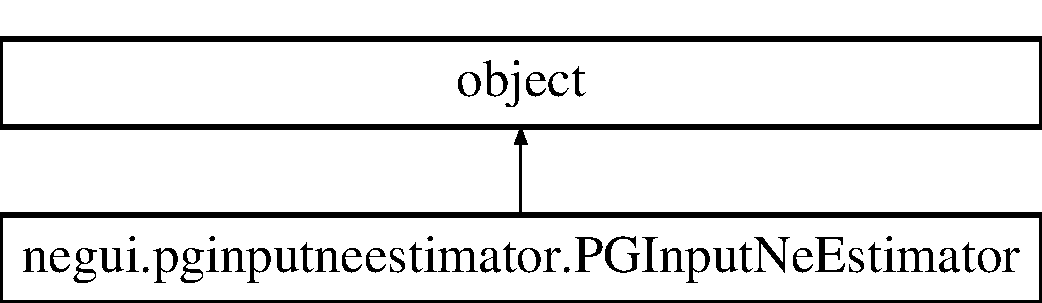
\includegraphics[height=2.000000cm]{classnegui_1_1pginputneestimator_1_1PGInputNeEstimator}
\end{center}
\end{figure}
\subsection*{Public Member Functions}
\begin{DoxyCompactItemize}
\item 
def {\bfseries \+\_\+\+\_\+init\+\_\+\+\_\+} (self, s\+\_\+genepop\+\_\+filename=None)\hypertarget{classnegui_1_1pginputneestimator_1_1PGInputNeEstimator_a88f248394897343472d0edf7c2e3ea3b}{}\label{classnegui_1_1pginputneestimator_1_1PGInputNeEstimator_a88f248394897343472d0edf7c2e3ea3b}

\item 
def {\bfseries genepop\+\_\+file} (self)\hypertarget{classnegui_1_1pginputneestimator_1_1PGInputNeEstimator_a3f32de00a24cc7a7dd28921697a58d4b}{}\label{classnegui_1_1pginputneestimator_1_1PGInputNeEstimator_a3f32de00a24cc7a7dd28921697a58d4b}

\item 
def {\bfseries run\+\_\+params} (self)\hypertarget{classnegui_1_1pginputneestimator_1_1PGInputNeEstimator_a87b6c321f810ee6efeee451958b92e56}{}\label{classnegui_1_1pginputneestimator_1_1PGInputNeEstimator_a87b6c321f810ee6efeee451958b92e56}

\item 
def {\bfseries run\+\_\+params} (self, dv\+\_\+params)\hypertarget{classnegui_1_1pginputneestimator_1_1PGInputNeEstimator_a1312da644290832102fb8937c38167bc}{}\label{classnegui_1_1pginputneestimator_1_1PGInputNeEstimator_a1312da644290832102fb8937c38167bc}

\end{DoxyCompactItemize}


\subsection{Detailed Description}
\begin{DoxyVerb}CLass to provide class PGOpNeEstimator
with input file and params needed to run
the ne-estimator object as coded in Tiago Antao's
ne2.py, one the age structure modules
\end{DoxyVerb}
 

Definition at line 12 of file pginputneestimator.\+py.



The documentation for this class was generated from the following file\+:\begin{DoxyCompactItemize}
\item 
pginputneestimator.\+py\end{DoxyCompactItemize}

\hypertarget{classnegui_1_1pginputsimupop_1_1PGInputSimuPop}{}\section{negui.\+pginputsimupop.\+P\+G\+Input\+Simu\+Pop Class Reference}
\label{classnegui_1_1pginputsimupop_1_1PGInputSimuPop}\index{negui.\+pginputsimupop.\+P\+G\+Input\+Simu\+Pop@{negui.\+pginputsimupop.\+P\+G\+Input\+Simu\+Pop}}
Inheritance diagram for negui.\+pginputsimupop.\+P\+G\+Input\+Simu\+Pop\+:\begin{figure}[H]
\begin{center}
\leavevmode
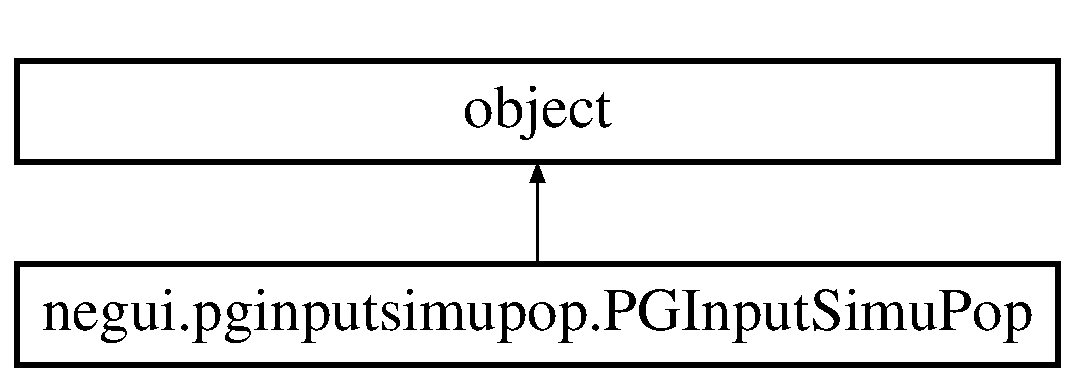
\includegraphics[height=2.000000cm]{classnegui_1_1pginputsimupop_1_1PGInputSimuPop}
\end{center}
\end{figure}
\subsection*{Public Member Functions}
\begin{DoxyCompactItemize}
\item 
def \hyperlink{classnegui_1_1pginputsimupop_1_1PGInputSimuPop_a1452a83a005c9d30e778b34ae67a399f}{\+\_\+\+\_\+init\+\_\+\+\_\+} (self, s\+\_\+config\+\_\+file=None, o\+\_\+model\+\_\+resources=None, o\+\_\+param\+\_\+names=None)
\item 
def {\bfseries setup\+Config\+Parser} (self, s\+\_\+config\+\_\+file\+\_\+name)\hypertarget{classnegui_1_1pginputsimupop_1_1PGInputSimuPop_a3f1295816cd5e708646d49e1d4f3fb1c}{}\label{classnegui_1_1pginputsimupop_1_1PGInputSimuPop_a3f1295816cd5e708646d49e1d4f3fb1c}

\item 
def {\bfseries get\+Config\+Parser\+Option} (self, s\+\_\+section\+\_\+name, s\+\_\+option\+\_\+name)\hypertarget{classnegui_1_1pginputsimupop_1_1PGInputSimuPop_abe1cda382edb5f59e3c01f2bee5b63c8}{}\label{classnegui_1_1pginputsimupop_1_1PGInputSimuPop_abe1cda382edb5f59e3c01f2bee5b63c8}

\item 
def \hyperlink{classnegui_1_1pginputsimupop_1_1PGInputSimuPop_aa990ef0c582a28a456a355a4eb3af2b9}{add\+Parameter} (self, s\+\_\+attribute\+\_\+name, v\+\_\+attribute\+\_\+value, s\+\_\+config\+\_\+file\+\_\+option\+\_\+name, s\+\_\+config\+\_\+file\+\_\+section\+\_\+name)
\item 
def {\bfseries get\+Dict\+Param\+Values\+By\+Attribute\+Name} (self)\hypertarget{classnegui_1_1pginputsimupop_1_1PGInputSimuPop_a099e2f01dabe86e713df7519a08fecca}{}\label{classnegui_1_1pginputsimupop_1_1PGInputSimuPop_a099e2f01dabe86e713df7519a08fecca}

\item 
def {\bfseries write\+Input\+Params\+To\+File\+Object} (self, o\+\_\+file)\hypertarget{classnegui_1_1pginputsimupop_1_1PGInputSimuPop_affc2fd6bd54b8f1ed84801b2f7f2da4b}{}\label{classnegui_1_1pginputsimupop_1_1PGInputSimuPop_affc2fd6bd54b8f1ed84801b2f7f2da4b}

\item 
def {\bfseries write\+Input\+Params\+As\+Config\+File} (self, s\+\_\+outfile\+\_\+name)\hypertarget{classnegui_1_1pginputsimupop_1_1PGInputSimuPop_a6264dda65b65dc05f2bb32a1c0be103d}{}\label{classnegui_1_1pginputsimupop_1_1PGInputSimuPop_a6264dda65b65dc05f2bb32a1c0be103d}

\item 
def {\bfseries make\+Input\+Config} (self)\hypertarget{classnegui_1_1pginputsimupop_1_1PGInputSimuPop_ac76cae13dbe53f4b69e9c287ee3f753c}{}\label{classnegui_1_1pginputsimupop_1_1PGInputSimuPop_ac76cae13dbe53f4b69e9c287ee3f753c}

\item 
def {\bfseries param\+\_\+names} (self)\hypertarget{classnegui_1_1pginputsimupop_1_1PGInputSimuPop_aa6402f6256dbac69f34b3a1bb4f6ccc5}{}\label{classnegui_1_1pginputsimupop_1_1PGInputSimuPop_aa6402f6256dbac69f34b3a1bb4f6ccc5}

\item 
def {\bfseries param\+\_\+names} (self, o\+\_\+param\+\_\+names)\hypertarget{classnegui_1_1pginputsimupop_1_1PGInputSimuPop_a02f3ff0a683450b071c6e4543c3c6211}{}\label{classnegui_1_1pginputsimupop_1_1PGInputSimuPop_a02f3ff0a683450b071c6e4543c3c6211}

\item 
def {\bfseries copy\+Me} (self)\hypertarget{classnegui_1_1pginputsimupop_1_1PGInputSimuPop_a9741a8266a14324ec7321121556fad24}{}\label{classnegui_1_1pginputsimupop_1_1PGInputSimuPop_a9741a8266a14324ec7321121556fad24}

\end{DoxyCompactItemize}
\subsection*{Public Attributes}
\begin{DoxyCompactItemize}
\item 
{\bfseries config\+\_\+file}\hypertarget{classnegui_1_1pginputsimupop_1_1PGInputSimuPop_af82bde7e564aee524fc30f2e06fde934}{}\label{classnegui_1_1pginputsimupop_1_1PGInputSimuPop_af82bde7e564aee524fc30f2e06fde934}

\item 
{\bfseries model\+\_\+name}\hypertarget{classnegui_1_1pginputsimupop_1_1PGInputSimuPop_aaa19ce0d9c031b5bdc97dc11f1523038}{}\label{classnegui_1_1pginputsimupop_1_1PGInputSimuPop_aaa19ce0d9c031b5bdc97dc11f1523038}

\item 
{\bfseries N0}\hypertarget{classnegui_1_1pginputsimupop_1_1PGInputSimuPop_a489012cc85bd8070c9ad118ff8655690}{}\label{classnegui_1_1pginputsimupop_1_1PGInputSimuPop_a489012cc85bd8070c9ad118ff8655690}

\item 
{\bfseries pop\+Size}\hypertarget{classnegui_1_1pginputsimupop_1_1PGInputSimuPop_aa777d14e980df9a76a3628cdea66f578}{}\label{classnegui_1_1pginputsimupop_1_1PGInputSimuPop_aa777d14e980df9a76a3628cdea66f578}

\item 
{\bfseries ages}\hypertarget{classnegui_1_1pginputsimupop_1_1PGInputSimuPop_ae2e25bf496108d9592d6f1ae20cbacc9}{}\label{classnegui_1_1pginputsimupop_1_1PGInputSimuPop_ae2e25bf496108d9592d6f1ae20cbacc9}

\item 
{\bfseries is\+Monog}\hypertarget{classnegui_1_1pginputsimupop_1_1PGInputSimuPop_ac7c254c11aab1479d06680b07358a52c}{}\label{classnegui_1_1pginputsimupop_1_1PGInputSimuPop_ac7c254c11aab1479d06680b07358a52c}

\item 
{\bfseries force\+Skip}\hypertarget{classnegui_1_1pginputsimupop_1_1PGInputSimuPop_ab8854f87f0ee0c762c4ad98bd09588ba}{}\label{classnegui_1_1pginputsimupop_1_1PGInputSimuPop_ab8854f87f0ee0c762c4ad98bd09588ba}

\item 
{\bfseries skip}\hypertarget{classnegui_1_1pginputsimupop_1_1PGInputSimuPop_ab3107ff3bc6fa8c2dd76de6ca9623369}{}\label{classnegui_1_1pginputsimupop_1_1PGInputSimuPop_ab3107ff3bc6fa8c2dd76de6ca9623369}

\item 
{\bfseries litter}\hypertarget{classnegui_1_1pginputsimupop_1_1PGInputSimuPop_a3a9a5714d275cfe4bf1d46268a253266}{}\label{classnegui_1_1pginputsimupop_1_1PGInputSimuPop_a3a9a5714d275cfe4bf1d46268a253266}

\item 
{\bfseries male\+Prob}\hypertarget{classnegui_1_1pginputsimupop_1_1PGInputSimuPop_a1bd24ef90fa7de0805492d5d280296b0}{}\label{classnegui_1_1pginputsimupop_1_1PGInputSimuPop_a1bd24ef90fa7de0805492d5d280296b0}

\item 
{\bfseries do\+Neg\+Binom}\hypertarget{classnegui_1_1pginputsimupop_1_1PGInputSimuPop_a3f8e03b3009323c0c71808eecf648a23}{}\label{classnegui_1_1pginputsimupop_1_1PGInputSimuPop_a3f8e03b3009323c0c71808eecf648a23}

\item 
{\bfseries gamma\+A\+Male}\hypertarget{classnegui_1_1pginputsimupop_1_1PGInputSimuPop_a05dd06f9deec5a92b87fd3bdb254da26}{}\label{classnegui_1_1pginputsimupop_1_1PGInputSimuPop_a05dd06f9deec5a92b87fd3bdb254da26}

\item 
{\bfseries gamma\+B\+Male}\hypertarget{classnegui_1_1pginputsimupop_1_1PGInputSimuPop_a0e221e1d44bc34027e3ea6f591ab47ba}{}\label{classnegui_1_1pginputsimupop_1_1PGInputSimuPop_a0e221e1d44bc34027e3ea6f591ab47ba}

\item 
{\bfseries gamma\+A\+Female}\hypertarget{classnegui_1_1pginputsimupop_1_1PGInputSimuPop_ad595aa7bd4560835e3e727b53efdde42}{}\label{classnegui_1_1pginputsimupop_1_1PGInputSimuPop_ad595aa7bd4560835e3e727b53efdde42}

\item 
{\bfseries gamma\+B\+Female}\hypertarget{classnegui_1_1pginputsimupop_1_1PGInputSimuPop_ae120c32c0e4f0636e0e30f7b0cc59260}{}\label{classnegui_1_1pginputsimupop_1_1PGInputSimuPop_ae120c32c0e4f0636e0e30f7b0cc59260}

\item 
{\bfseries survival\+Male}\hypertarget{classnegui_1_1pginputsimupop_1_1PGInputSimuPop_ac2fd3ccd92e7fdf55d754b07a359bb8b}{}\label{classnegui_1_1pginputsimupop_1_1PGInputSimuPop_ac2fd3ccd92e7fdf55d754b07a359bb8b}

\item 
{\bfseries survival\+Female}\hypertarget{classnegui_1_1pginputsimupop_1_1PGInputSimuPop_ae01eb4e5af6a562f0fd7260f178bec87}{}\label{classnegui_1_1pginputsimupop_1_1PGInputSimuPop_ae01eb4e5af6a562f0fd7260f178bec87}

\item 
{\bfseries fecundity\+Male}\hypertarget{classnegui_1_1pginputsimupop_1_1PGInputSimuPop_acbca25eadad7f1591c9072843bb23952}{}\label{classnegui_1_1pginputsimupop_1_1PGInputSimuPop_acbca25eadad7f1591c9072843bb23952}

\item 
{\bfseries fecundity\+Female}\hypertarget{classnegui_1_1pginputsimupop_1_1PGInputSimuPop_a7baba0908f0d1fea5e9284d1b8649e10}{}\label{classnegui_1_1pginputsimupop_1_1PGInputSimuPop_a7baba0908f0d1fea5e9284d1b8649e10}

\item 
{\bfseries start\+Lambda}\hypertarget{classnegui_1_1pginputsimupop_1_1PGInputSimuPop_a0139fdc38fda73d6570fa05850608754}{}\label{classnegui_1_1pginputsimupop_1_1PGInputSimuPop_a0139fdc38fda73d6570fa05850608754}

\item 
{\bfseries lbd}\hypertarget{classnegui_1_1pginputsimupop_1_1PGInputSimuPop_aa89e1f6520b205495fd8182ace5b38aa}{}\label{classnegui_1_1pginputsimupop_1_1PGInputSimuPop_aa89e1f6520b205495fd8182ace5b38aa}

\item 
{\bfseries Nb}\hypertarget{classnegui_1_1pginputsimupop_1_1PGInputSimuPop_a44d7c54334644d2f7131580e4173b789}{}\label{classnegui_1_1pginputsimupop_1_1PGInputSimuPop_a44d7c54334644d2f7131580e4173b789}

\item 
{\bfseries Nb\+Var}\hypertarget{classnegui_1_1pginputsimupop_1_1PGInputSimuPop_acdeba096bc557395a8e6d03651e3da2f}{}\label{classnegui_1_1pginputsimupop_1_1PGInputSimuPop_acdeba096bc557395a8e6d03651e3da2f}

\item 
{\bfseries start\+Alleles}\hypertarget{classnegui_1_1pginputsimupop_1_1PGInputSimuPop_a551d4203e5bcc9ce2925be0fe4947e7b}{}\label{classnegui_1_1pginputsimupop_1_1PGInputSimuPop_a551d4203e5bcc9ce2925be0fe4947e7b}

\item 
{\bfseries mut\+Freq}\hypertarget{classnegui_1_1pginputsimupop_1_1PGInputSimuPop_abe92e0c080a608ce45880f5257f5fbfe}{}\label{classnegui_1_1pginputsimupop_1_1PGInputSimuPop_abe92e0c080a608ce45880f5257f5fbfe}

\item 
{\bfseries num\+M\+Sats}\hypertarget{classnegui_1_1pginputsimupop_1_1PGInputSimuPop_a5b562f2c6c9fd905e1f8e9c05611f62b}{}\label{classnegui_1_1pginputsimupop_1_1PGInputSimuPop_a5b562f2c6c9fd905e1f8e9c05611f62b}

\item 
{\bfseries num\+S\+N\+Ps}\hypertarget{classnegui_1_1pginputsimupop_1_1PGInputSimuPop_a1125f77d55338c88bf0d4bce14d90f5b}{}\label{classnegui_1_1pginputsimupop_1_1PGInputSimuPop_a1125f77d55338c88bf0d4bce14d90f5b}

\item 
{\bfseries reps}\hypertarget{classnegui_1_1pginputsimupop_1_1PGInputSimuPop_ad9123c2163f7ab6a1e0903bd63316ca6}{}\label{classnegui_1_1pginputsimupop_1_1PGInputSimuPop_ad9123c2163f7ab6a1e0903bd63316ca6}

\item 
{\bfseries start\+Save}\hypertarget{classnegui_1_1pginputsimupop_1_1PGInputSimuPop_a73ab30f9db93cfbd18580023886774d8}{}\label{classnegui_1_1pginputsimupop_1_1PGInputSimuPop_a73ab30f9db93cfbd18580023886774d8}

\item 
{\bfseries gens}\hypertarget{classnegui_1_1pginputsimupop_1_1PGInputSimuPop_aceb30da861b01f9f89e7b2d1fe78ba32}{}\label{classnegui_1_1pginputsimupop_1_1PGInputSimuPop_aceb30da861b01f9f89e7b2d1fe78ba32}

\item 
{\bfseries data\+Dir}\hypertarget{classnegui_1_1pginputsimupop_1_1PGInputSimuPop_a423a2c1ac08af8ba57663207700e5796}{}\label{classnegui_1_1pginputsimupop_1_1PGInputSimuPop_a423a2c1ac08af8ba57663207700e5796}

\end{DoxyCompactItemize}


\subsection{Detailed Description}
\begin{DoxyVerb}Object meant to fetch parameter values and prepare them for 
use in a simuPop simulation.  

Object to be passed to a PGOpSimuPop object, which is, in turn,
passed to a PGGuiSimuPop object, so that the widgets can then access
defs in this input object, in order to, for example, show or allow
changes in parameter values for users before they run the simulation.
\end{DoxyVerb}
 

Definition at line 15 of file pginputsimupop.\+py.



\subsection{Constructor \& Destructor Documentation}
\index{negui\+::pginputsimupop\+::\+P\+G\+Input\+Simu\+Pop@{negui\+::pginputsimupop\+::\+P\+G\+Input\+Simu\+Pop}!\+\_\+\+\_\+init\+\_\+\+\_\+@{\+\_\+\+\_\+init\+\_\+\+\_\+}}
\index{\+\_\+\+\_\+init\+\_\+\+\_\+@{\+\_\+\+\_\+init\+\_\+\+\_\+}!negui\+::pginputsimupop\+::\+P\+G\+Input\+Simu\+Pop@{negui\+::pginputsimupop\+::\+P\+G\+Input\+Simu\+Pop}}
\subsubsection[{\texorpdfstring{\+\_\+\+\_\+init\+\_\+\+\_\+(self, s\+\_\+config\+\_\+file=\+None, o\+\_\+model\+\_\+resources=\+None, o\+\_\+param\+\_\+names=\+None)}{__init__(self, s_config_file=None, o_model_resources=None, o_param_names=None)}}]{\setlength{\rightskip}{0pt plus 5cm}def negui.\+pginputsimupop.\+P\+G\+Input\+Simu\+Pop.\+\_\+\+\_\+init\+\_\+\+\_\+ (
\begin{DoxyParamCaption}
\item[{}]{self, }
\item[{}]{s\+\_\+config\+\_\+file = {\ttfamily None}, }
\item[{}]{o\+\_\+model\+\_\+resources = {\ttfamily None}, }
\item[{}]{o\+\_\+param\+\_\+names = {\ttfamily None}}
\end{DoxyParamCaption}
)}\hypertarget{classnegui_1_1pginputsimupop_1_1PGInputSimuPop_a1452a83a005c9d30e778b34ae67a399f}{}\label{classnegui_1_1pginputsimupop_1_1PGInputSimuPop_a1452a83a005c9d30e778b34ae67a399f}
\begin{DoxyVerb}param s_config_file, parseable by ConfigParser, params for 
    running simuPop, or references into the resources
    object.  Note that this config file must have a
    section called "model" with a "name" option, which
    should match a name key in the PGModelResources objects
    dictionary.

param o_model_resources, object of type PGModelResources,
    whose member dictionary has the sub-dictionaries
    that have the param values not given in the config file,
    such as fecundity and reproductive values, and exposed
    via calls to is getValue def.

param o_param_names, object ot type PGParamSet,
    that gives a shortname (attribute name)
    and a longname (readable text), for each 
    param in the simpupop configuration attribute 
    list
\end{DoxyVerb}
 

Definition at line 25 of file pginputsimupop.\+py.


\begin{DoxyCode}
25     \textcolor{keyword}{def }\hyperlink{classnegui_1_1pginputsimupop_1_1PGInputSimuPop_a1452a83a005c9d30e778b34ae67a399f}{\_\_init\_\_}( self, s\_config\_file = None, o\_model\_resources = None, o\_param\_names=None ):
26         \textcolor{stringliteral}{'''}
27 \textcolor{stringliteral}{        param s\_config\_file, parseable by ConfigParser, params for }
28 \textcolor{stringliteral}{            running simuPop, or references into the resources}
29 \textcolor{stringliteral}{            object.  Note that this config file must have a}
30 \textcolor{stringliteral}{            section called "model" with a "name" option, which}
31 \textcolor{stringliteral}{            should match a name key in the PGModelResources objects}
32 \textcolor{stringliteral}{            dictionary.}
33 \textcolor{stringliteral}{}
34 \textcolor{stringliteral}{        param o\_model\_resources, object of type PGModelResources,}
35 \textcolor{stringliteral}{            whose member dictionary has the sub-dictionaries}
36 \textcolor{stringliteral}{            that have the param values not given in the config file,}
37 \textcolor{stringliteral}{            such as fecundity and reproductive values, and exposed}
38 \textcolor{stringliteral}{            via calls to is getValue def.}
39 \textcolor{stringliteral}{}
40 \textcolor{stringliteral}{        param o\_param\_names, object ot type PGParamSet,}
41 \textcolor{stringliteral}{            that gives a shortname (attribute name)}
42 \textcolor{stringliteral}{            and a longname (readable text), for each }
43 \textcolor{stringliteral}{            param in the simpupop configuration attribute }
44 \textcolor{stringliteral}{            list}
45 \textcolor{stringliteral}{        '''}
46 
47         self.\hyperlink{classnegui_1_1pginputsimupop_1_1PGInputSimuPop_af6628ecaa63a594fc96d1b9273fd1fd6}{\_\_config\_parser}=\textcolor{keywordtype}{None}
48         self.\hyperlink{classnegui_1_1pginputsimupop_1_1PGInputSimuPop_a6c00be5e58b61b239273e04c671cd9e8}{\_\_resources}=o\_model\_resources
49         self.\hyperlink{classnegui_1_1pginputsimupop_1_1PGInputSimuPop_a0a737393cb4d1c66062f9403296c7f19}{\_\_param\_names}=o\_param\_names
50 
51         \textcolor{comment}{#for writing current param values to a new config file,}
52         \textcolor{comment}{#and updated as attributes are created either by reading}
53         \textcolor{comment}{#in the orig config file in def get\_config, or by adding the parameter}
54         \textcolor{comment}{#in def addParameter:}
55         self.\hyperlink{classnegui_1_1pginputsimupop_1_1PGInputSimuPop_a893ab501191e9e1ed89f4f878310d97b}{\_\_config\_file\_option\_name\_by\_attribute\_name}=\{\}      
56         self.\hyperlink{classnegui_1_1pginputsimupop_1_1PGInputSimuPop_acd9740f17e53a6e471d4e85565962369}{\_\_config\_file\_section\_name\_by\_attribute\_name}=\{\}
57 
58         \textcolor{keywordflow}{if} s\_config\_file \textcolor{keywordflow}{is} \textcolor{keywordflow}{not} \textcolor{keywordtype}{None}:
59             self.\hyperlink{classnegui_1_1pginputsimupop_1_1PGInputSimuPop_ad7c3feef55c16989a35f56c3e0d9943e}{\_\_full\_config\_file\_name}=s\_config\_file
60             self.\hyperlink{classnegui_1_1pginputsimupop_1_1PGInputSimuPop_af82bde7e564aee524fc30f2e06fde934}{config\_file}=os.path.basename( s\_config\_file )
61             self.\hyperlink{classnegui_1_1pginputsimupop_1_1PGInputSimuPop_a0b34c99730e86de268c5503ed226d15e}{\_\_make\_config\_parser}( s\_config\_file )
62         \textcolor{comment}{#end if we have a conf file}
63 
64         \textcolor{keywordflow}{return}
\end{DoxyCode}


\subsection{Member Function Documentation}
\index{negui\+::pginputsimupop\+::\+P\+G\+Input\+Simu\+Pop@{negui\+::pginputsimupop\+::\+P\+G\+Input\+Simu\+Pop}!add\+Parameter@{add\+Parameter}}
\index{add\+Parameter@{add\+Parameter}!negui\+::pginputsimupop\+::\+P\+G\+Input\+Simu\+Pop@{negui\+::pginputsimupop\+::\+P\+G\+Input\+Simu\+Pop}}
\subsubsection[{\texorpdfstring{add\+Parameter(self, s\+\_\+attribute\+\_\+name, v\+\_\+attribute\+\_\+value, s\+\_\+config\+\_\+file\+\_\+option\+\_\+name, s\+\_\+config\+\_\+file\+\_\+section\+\_\+name)}{addParameter(self, s_attribute_name, v_attribute_value, s_config_file_option_name, s_config_file_section_name)}}]{\setlength{\rightskip}{0pt plus 5cm}def negui.\+pginputsimupop.\+P\+G\+Input\+Simu\+Pop.\+add\+Parameter (
\begin{DoxyParamCaption}
\item[{}]{self, }
\item[{}]{s\+\_\+attribute\+\_\+name, }
\item[{}]{v\+\_\+attribute\+\_\+value, }
\item[{}]{s\+\_\+config\+\_\+file\+\_\+option\+\_\+name, }
\item[{}]{s\+\_\+config\+\_\+file\+\_\+section\+\_\+name}
\end{DoxyParamCaption}
)}\hypertarget{classnegui_1_1pginputsimupop_1_1PGInputSimuPop_aa990ef0c582a28a456a355a4eb3af2b9}{}\label{classnegui_1_1pginputsimupop_1_1PGInputSimuPop_aa990ef0c582a28a456a355a4eb3af2b9}
\begin{DoxyVerb}If user wants to add a parameter not in the current set of params as read
in from the config file source of this instance, this def will both add the 
param and value, plus update the member dictionaries that facilitate
writing a new config file that includes this parameter.  Note that the
arg s_config_file_option_name is necessitated by Tiago's standards in 
his config files, as he often uses an attribute name different
from the option name that gives the value.
\end{DoxyVerb}
 

Definition at line 311 of file pginputsimupop.\+py.


\begin{DoxyCode}
311             s\_config\_file\_section\_name ):
312         \textcolor{stringliteral}{'''}
313 \textcolor{stringliteral}{        If user wants to add a parameter not in the current set of params as read}
314 \textcolor{stringliteral}{        in from the config file source of this instance, this def will both add the }
315 \textcolor{stringliteral}{        param and value, plus update the member dictionaries that facilitate}
316 \textcolor{stringliteral}{        writing a new config file that includes this parameter.  Note that the}
317 \textcolor{stringliteral}{        arg s\_config\_file\_option\_name is necessitated by Tiago's standards in }
318 \textcolor{stringliteral}{        his config files, as he often uses an attribute name different}
319 \textcolor{stringliteral}{        from the option name that gives the value.}
320 \textcolor{stringliteral}{        '''}
321         setattr( self, s\_attribute\_name, v\_attribute\_value )
322         self.\hyperlink{classnegui_1_1pginputsimupop_1_1PGInputSimuPop_a27abd811d6b6108a9593372c3b0c7881}{\_\_update\_attribute\_config\_file\_info}( s\_attribute\_name, 
      s\_config\_file\_section\_name, 
323                 s\_config\_file\_option\_name )
324         \textcolor{keywordflow}{return}
\end{DoxyCode}


The documentation for this class was generated from the following file\+:\begin{DoxyCompactItemize}
\item 
pginputsimupop.\+py\end{DoxyCompactItemize}

\hypertarget{classnegui_1_1pgmenubuilder_1_1PGMenuBuilder}{}\section{negui.\+pgmenubuilder.\+P\+G\+Menu\+Builder Class Reference}
\label{classnegui_1_1pgmenubuilder_1_1PGMenuBuilder}\index{negui.\+pgmenubuilder.\+P\+G\+Menu\+Builder@{negui.\+pgmenubuilder.\+P\+G\+Menu\+Builder}}
Inheritance diagram for negui.\+pgmenubuilder.\+P\+G\+Menu\+Builder\+:\begin{figure}[H]
\begin{center}
\leavevmode
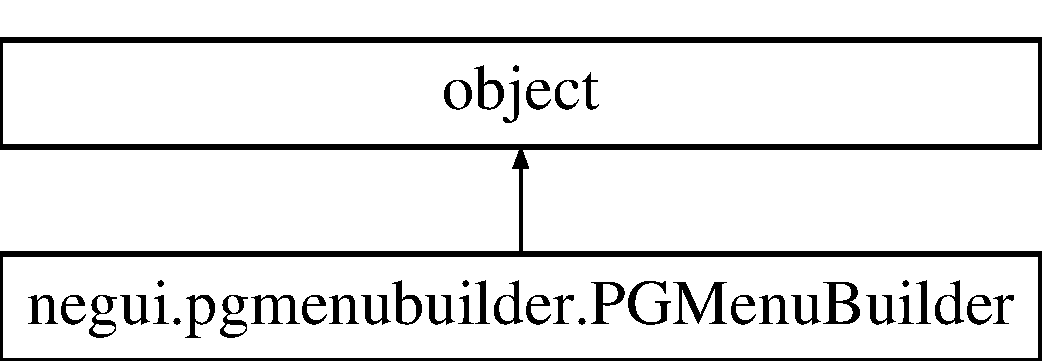
\includegraphics[height=2.000000cm]{classnegui_1_1pgmenubuilder_1_1PGMenuBuilder}
\end{center}
\end{figure}
\subsection*{Public Member Functions}
\begin{DoxyCompactItemize}
\item 
def \hyperlink{classnegui_1_1pgmenubuilder_1_1PGMenuBuilder_a8e612e54bfe556d763a7150d8d8cbec5}{\+\_\+\+\_\+init\+\_\+\+\_\+} (self, s\+\_\+config\+\_\+file, o\+\_\+pg\+\_\+gui\+\_\+app, o\+\_\+tk\+\_\+master, i\+\_\+tearoff=0)
\item 
def \hyperlink{classnegui_1_1pgmenubuilder_1_1PGMenuBuilder_a564a7629d3ba8ac1666a6f8a046d82f2}{get\+\_\+add\+\_\+command\+\_\+params\+\_\+and\+\_\+args} (self, o\+\_\+config, s\+\_\+menu\+\_\+label)
\item 
def \hyperlink{classnegui_1_1pgmenubuilder_1_1PGMenuBuilder_ae45f68f11cc8fa8c39d8b93a15238c83}{menu} (self)
\item 
def {\bfseries menu} (self, i\+\_\+value)\hypertarget{classnegui_1_1pgmenubuilder_1_1PGMenuBuilder_a286f1b5420d31d737f0680926e4f0fa3}{}\label{classnegui_1_1pgmenubuilder_1_1PGMenuBuilder_a286f1b5420d31d737f0680926e4f0fa3}

\item 
def {\bfseries menu} (self)\hypertarget{classnegui_1_1pgmenubuilder_1_1PGMenuBuilder_ae45f68f11cc8fa8c39d8b93a15238c83}{}\label{classnegui_1_1pgmenubuilder_1_1PGMenuBuilder_ae45f68f11cc8fa8c39d8b93a15238c83}

\end{DoxyCompactItemize}
\subsection*{Static Public Attributes}
\begin{DoxyCompactItemize}
\item 
list {\bfseries C\+O\+N\+F\+I\+G\+\_\+\+O\+P\+T\+I\+O\+N\+S\+\_\+\+N\+O\+N\+\_\+\+C\+O\+M\+M\+A\+N\+D\+\_\+\+A\+R\+GS} = \mbox{[} \char`\"{}parent\char`\"{}, \char`\"{}menu\+\_\+underline\char`\"{}, \char`\"{}menu\+\_\+accelerator\char`\"{} \mbox{]}\hypertarget{classnegui_1_1pgmenubuilder_1_1PGMenuBuilder_ae546003717fb9974243ea7bd53540e4e}{}\label{classnegui_1_1pgmenubuilder_1_1PGMenuBuilder_ae546003717fb9974243ea7bd53540e4e}

\end{DoxyCompactItemize}


\subsection{Detailed Description}
\begin{DoxyVerb}Instantiates a tkinter menu_bar, with parent gui object (usually the main window) 
as given by __init__ param, and populates it by reading a list of menu items and 
parameters from a configuration file, also an __init__ param. The menus get their 
command callback defs, as named in the configuration file, in the class object 
passed as init param o_pg_gui_app.

The configuration file key=value entries inside each [section] are of two classes:

1. keys that are not param keywords for the call to menu.add_command.  These include 
    (a) "parent=value", which tells the
    builder which of the file labels (sections in the config file) is the parent menu
    to it's submenu.  As of 20160116 this is not implemented, and only parent=None (unquoted) 
    is allowed.
    (b) "menu_underline=value", where value is an (zero-based) index into the menu label name 
    (as given by the section name).

2. key=value pairs whose keys are param keywords (like "accelerator").  Keys must match exactly
    prarm names in the menu.add_command definition's param list.  Their values should be 
    entered in square brackets like a python list, with one entry for each of the menu items.  
    If the nth item is to be "seperator" item, the nth item in the label list should be 
    "sep", and other items like "command" or accelerator, can be any value (ex: None), 
    as they will be ignored.

For example, a menubar with 2 items "File" and "Edit", each with 2 menu items, with
Edit having a seperator between its items would look like this: 

#file menu
[File]
parent=None
#which characters to underline in the File label:
menu_underline=0
label=[ "New" , "Open" ]
#which characters to underline in the menu items:
underline=[ 0, 0 ]
accelerator=[ "Ctrl+N","Ctrl+O" ]
command=[ "new_file", "open_file" ]

#edit menu
[Edit]
parent=None
menu_underline=0
label=["Undo","sep","Options"]
underline=[ 1,None, 1 ]
accelerator=["Ctrl+Z", None, "Ctrl+T"]
command=[ "undo", None, "showopts" ]  
\end{DoxyVerb}
 

Definition at line 16 of file pgmenubuilder.\+py.



\subsection{Constructor \& Destructor Documentation}
\index{negui\+::pgmenubuilder\+::\+P\+G\+Menu\+Builder@{negui\+::pgmenubuilder\+::\+P\+G\+Menu\+Builder}!\+\_\+\+\_\+init\+\_\+\+\_\+@{\+\_\+\+\_\+init\+\_\+\+\_\+}}
\index{\+\_\+\+\_\+init\+\_\+\+\_\+@{\+\_\+\+\_\+init\+\_\+\+\_\+}!negui\+::pgmenubuilder\+::\+P\+G\+Menu\+Builder@{negui\+::pgmenubuilder\+::\+P\+G\+Menu\+Builder}}
\subsubsection[{\texorpdfstring{\+\_\+\+\_\+init\+\_\+\+\_\+(self, s\+\_\+config\+\_\+file, o\+\_\+pg\+\_\+gui\+\_\+app, o\+\_\+tk\+\_\+master, i\+\_\+tearoff=0)}{__init__(self, s_config_file, o_pg_gui_app, o_tk_master, i_tearoff=0)}}]{\setlength{\rightskip}{0pt plus 5cm}def negui.\+pgmenubuilder.\+P\+G\+Menu\+Builder.\+\_\+\+\_\+init\+\_\+\+\_\+ (
\begin{DoxyParamCaption}
\item[{}]{self, }
\item[{}]{s\+\_\+config\+\_\+file, }
\item[{}]{o\+\_\+pg\+\_\+gui\+\_\+app, }
\item[{}]{o\+\_\+tk\+\_\+master, }
\item[{}]{i\+\_\+tearoff = {\ttfamily 0}}
\end{DoxyParamCaption}
)}\hypertarget{classnegui_1_1pgmenubuilder_1_1PGMenuBuilder_a8e612e54bfe556d763a7150d8d8cbec5}{}\label{classnegui_1_1pgmenubuilder_1_1PGMenuBuilder_a8e612e54bfe556d763a7150d8d8cbec5}
\begin{DoxyVerb}param s_config_file gives menu attribute values (see module documentation)
param o_pg_gui_app is a class object that has the definitions
that match the command names to be bound to the menus ('command' 
option values in the config file). It also has a member Tk()
root window object that the menu builder assigns to member "parent"
param i_tearoff tells the gui whether the menu items can be dragged off of 
    the parent menubar (tearoff=1) or not (tearoff=0)
\end{DoxyVerb}
 

Definition at line 67 of file pgmenubuilder.\+py.


\begin{DoxyCode}
67     \textcolor{keyword}{def }\hyperlink{classnegui_1_1pgmenubuilder_1_1PGMenuBuilder_a8e612e54bfe556d763a7150d8d8cbec5}{\_\_init\_\_}( self, s\_config\_file, o\_pg\_gui\_app,  o\_tk\_master, i\_tearoff=0 ):
68         \textcolor{stringliteral}{'''}
69 \textcolor{stringliteral}{        param s\_config\_file gives menu attribute values (see module documentation)}
70 \textcolor{stringliteral}{        param o\_pg\_gui\_app is a class object that has the definitions}
71 \textcolor{stringliteral}{                that match the command names to be bound to the menus ('command' }
72 \textcolor{stringliteral}{                option values in the config file). It also has a member Tk()}
73 \textcolor{stringliteral}{                root window object that the menu builder assigns to member "parent"}
74 \textcolor{stringliteral}{        param i\_tearoff tells the gui whether the menu items can be dragged off of }
75 \textcolor{stringliteral}{            the parent menubar (tearoff=1) or not (tearoff=0)}
76 \textcolor{stringliteral}{        '''}
77         self.\hyperlink{classnegui_1_1pgmenubuilder_1_1PGMenuBuilder_ae68d0c5a32a42f23fae44d177125e639}{\_\_menubar} = \textcolor{keywordtype}{None}
78         self.\hyperlink{classnegui_1_1pgmenubuilder_1_1PGMenuBuilder_af0a1a02f4ae4cb51ddcae82ff1bda3b8}{\_\_pg\_gui\_app} = o\_pg\_gui\_app
79         self.\hyperlink{classnegui_1_1pgmenubuilder_1_1PGMenuBuilder_aa1c29f9898f4129fa7a8c3fa52498322}{\_\_tearoff} = i\_tearoff
80         self.\hyperlink{classnegui_1_1pgmenubuilder_1_1PGMenuBuilder_a96fdfb4d4b5bfc2cb502ca5c513f4326}{\_\_parent}=o\_tk\_master
81         o\_config = self.\hyperlink{classnegui_1_1pgmenubuilder_1_1PGMenuBuilder_af9e8faf1c4c173851774fb37f0900a2c}{\_\_get\_menu\_info}( s\_config\_file )
82         self.\hyperlink{classnegui_1_1pgmenubuilder_1_1PGMenuBuilder_a308e619e77dc646c8668bbced4171394}{\_\_build\_menu}( o\_config )
83         \textcolor{keywordflow}{return}
\end{DoxyCode}


\subsection{Member Function Documentation}
\index{negui\+::pgmenubuilder\+::\+P\+G\+Menu\+Builder@{negui\+::pgmenubuilder\+::\+P\+G\+Menu\+Builder}!get\+\_\+add\+\_\+command\+\_\+params\+\_\+and\+\_\+args@{get\+\_\+add\+\_\+command\+\_\+params\+\_\+and\+\_\+args}}
\index{get\+\_\+add\+\_\+command\+\_\+params\+\_\+and\+\_\+args@{get\+\_\+add\+\_\+command\+\_\+params\+\_\+and\+\_\+args}!negui\+::pgmenubuilder\+::\+P\+G\+Menu\+Builder@{negui\+::pgmenubuilder\+::\+P\+G\+Menu\+Builder}}
\subsubsection[{\texorpdfstring{get\+\_\+add\+\_\+command\+\_\+params\+\_\+and\+\_\+args(self, o\+\_\+config, s\+\_\+menu\+\_\+label)}{get_add_command_params_and_args(self, o_config, s_menu_label)}}]{\setlength{\rightskip}{0pt plus 5cm}def negui.\+pgmenubuilder.\+P\+G\+Menu\+Builder.\+get\+\_\+add\+\_\+command\+\_\+params\+\_\+and\+\_\+args (
\begin{DoxyParamCaption}
\item[{}]{self, }
\item[{}]{o\+\_\+config, }
\item[{}]{s\+\_\+menu\+\_\+label}
\end{DoxyParamCaption}
)}\hypertarget{classnegui_1_1pgmenubuilder_1_1PGMenuBuilder_a564a7629d3ba8ac1666a6f8a046d82f2}{}\label{classnegui_1_1pgmenubuilder_1_1PGMenuBuilder_a564a7629d3ba8ac1666a6f8a046d82f2}
\begin{DoxyVerb}returns a list of dictionaries, one for each menu item, of the param=value
settings for calls to menu.add_command.  We skip the config key=value for keys
that are not part of the params needed for add_command. 
\end{DoxyVerb}
 

Definition at line 126 of file pgmenubuilder.\+py.


\begin{DoxyCode}
126     \textcolor{keyword}{def }\hyperlink{classnegui_1_1pgmenubuilder_1_1PGMenuBuilder_a564a7629d3ba8ac1666a6f8a046d82f2}{get\_add\_command\_params\_and\_args}( self,  o\_config, s\_menu\_label ):
127         \textcolor{stringliteral}{'''}
128 \textcolor{stringliteral}{        returns a list of dictionaries, one for each menu item, of the param=value}
129 \textcolor{stringliteral}{        settings for calls to menu.add\_command.  We skip the config key=value for keys}
130 \textcolor{stringliteral}{        that are not part of the params needed for add\_command. }
131 \textcolor{stringliteral}{        '''}
132         l\_keyword\_menu\_params = o\_config.options( s\_menu\_label )    
133 
134         \textcolor{comment}{#how many items on this menu should equal number of labels:}
135         i\_num\_items = self.\hyperlink{classnegui_1_1pgmenubuilder_1_1PGMenuBuilder_a70776ac09761aeef9ee6df67c1dd9140}{\_\_get\_num\_labels\_menu}( o\_config, s\_menu\_label )
136 
137         ld\_args = [ \{\} \textcolor{keywordflow}{for} idx \textcolor{keywordflow}{in} range( i\_num\_items ) ]
138 
139         \textcolor{comment}{#for each submenu item, we get a dict of keyword:value to pass to "add\_command"}
140         \textcolor{keywordflow}{for} s\_keyword \textcolor{keywordflow}{in} l\_keyword\_menu\_params:
141             s\_vals=o\_config.get( s\_menu\_label, s\_keyword )
142 
143             \textcolor{comment}{#for each keyword that is a param name in the menu.add\_command call}
144             \textcolor{keywordflow}{if} s\_keyword \textcolor{keywordflow}{not} \textcolor{keywordflow}{in} PGMenuBuilder.CONFIG\_OPTIONS\_NON\_COMMAND\_ARGS:
145 
146                 l\_vals=eval( s\_vals )
147 
148                 \textcolor{keywordflow}{if} len( l\_vals ) != i\_num\_items:
149                     \textcolor{keywordflow}{raise} Exception( \textcolor{stringliteral}{"in pgmenubuilder, config entry should have "} \(\backslash\)
150                             + \textcolor{stringliteral}{"one item for each label, but the option with keyname, "} \(\backslash\)
151                             + s\_keyword + \textcolor{stringliteral}{" does not."} )
152                 \textcolor{comment}{#end if wrong number values}
153                 
154                 \textcolor{comment}{#if this is the list of command values (callback defs) }
155                 \textcolor{comment}{#for each submenu item,}
156                 \textcolor{comment}{#then we must be able to find it among the attributes}
157                 \textcolor{comment}{#of our member operation object}
158                 \textcolor{comment}{#note: if "sep" is the label, we set other param values }
159                 \textcolor{comment}{#to None, but they are ignored (see for loop below)}
160                 \textcolor{keywordflow}{if} s\_keyword ==\textcolor{stringliteral}{"command"}:
161                     l\_vals = [ getattr( self.\hyperlink{classnegui_1_1pgmenubuilder_1_1PGMenuBuilder_af0a1a02f4ae4cb51ddcae82ff1bda3b8}{\_\_pg\_gui\_app}, thisval ) \(\backslash\)
162                             \textcolor{keywordflow}{if} thisval \textcolor{keywordflow}{is} \textcolor{keywordflow}{not} \textcolor{keywordtype}{None} \(\backslash\)
163                             \textcolor{keywordflow}{else} \textcolor{keywordtype}{None} \textcolor{keywordflow}{for} thisval \textcolor{keywordflow}{in} l\_vals ]
164                 \textcolor{comment}{#end if command list}
165 
166                 \textcolor{keywordflow}{for} idx \textcolor{keywordflow}{in} range( i\_num\_items ):
167                     ld\_args[ idx ][ s\_keyword ] = l\_vals[ idx ]
168                 \textcolor{comment}{#end for each item}
169             \textcolor{comment}{#end if not a param keyword for add\_command}
170         \textcolor{comment}{#end for each keyword}
171 
172         \textcolor{keywordflow}{return} ld\_args
\end{DoxyCode}
\index{negui\+::pgmenubuilder\+::\+P\+G\+Menu\+Builder@{negui\+::pgmenubuilder\+::\+P\+G\+Menu\+Builder}!menu@{menu}}
\index{menu@{menu}!negui\+::pgmenubuilder\+::\+P\+G\+Menu\+Builder@{negui\+::pgmenubuilder\+::\+P\+G\+Menu\+Builder}}
\subsubsection[{\texorpdfstring{menu(self)}{menu(self)}}]{\setlength{\rightskip}{0pt plus 5cm}def negui.\+pgmenubuilder.\+P\+G\+Menu\+Builder.\+menu (
\begin{DoxyParamCaption}
\item[{}]{self}
\end{DoxyParamCaption}
)}\hypertarget{classnegui_1_1pgmenubuilder_1_1PGMenuBuilder_ae45f68f11cc8fa8c39d8b93a15238c83}{}\label{classnegui_1_1pgmenubuilder_1_1PGMenuBuilder_ae45f68f11cc8fa8c39d8b93a15238c83}
\begin{DoxyVerb}menu, tk.TKMenu object\end{DoxyVerb}
 

Definition at line 244 of file pgmenubuilder.\+py.


\begin{DoxyCode}
244     \textcolor{keyword}{def }\hyperlink{classnegui_1_1pgmenubuilder_1_1PGMenuBuilder_ae45f68f11cc8fa8c39d8b93a15238c83}{menu}(self):
245         \textcolor{stringliteral}{"""menu, tk.TKMenu object"""}
246         \textcolor{keywordflow}{return} self.\hyperlink{classnegui_1_1pgmenubuilder_1_1PGMenuBuilder_ae68d0c5a32a42f23fae44d177125e639}{\_\_menubar}
\end{DoxyCode}


The documentation for this class was generated from the following file\+:\begin{DoxyCompactItemize}
\item 
pgmenubuilder.\+py\end{DoxyCompactItemize}

\hypertarget{classnegui_1_1pgopneestimator_1_1PGOpNeEstimator}{}\section{negui.\+pgopneestimator.\+P\+G\+Op\+Ne\+Estimator Class Reference}
\label{classnegui_1_1pgopneestimator_1_1PGOpNeEstimator}\index{negui.\+pgopneestimator.\+P\+G\+Op\+Ne\+Estimator@{negui.\+pgopneestimator.\+P\+G\+Op\+Ne\+Estimator}}
Inheritance diagram for negui.\+pgopneestimator.\+P\+G\+Op\+Ne\+Estimator\+:\begin{figure}[H]
\begin{center}
\leavevmode
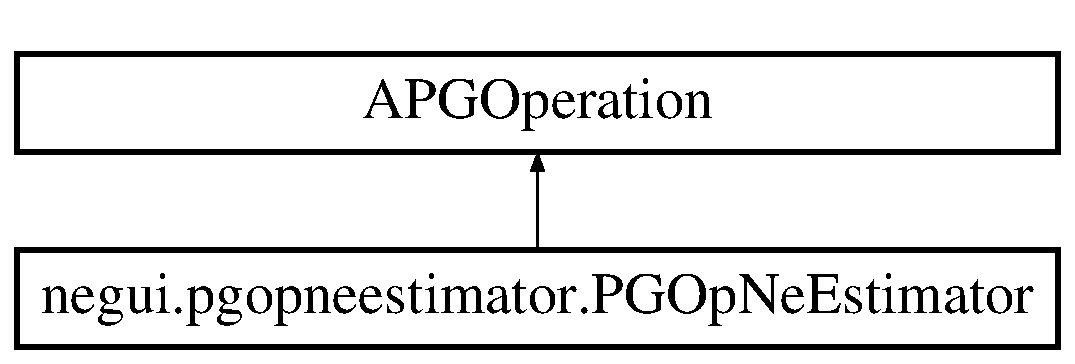
\includegraphics[height=2.000000cm]{classnegui_1_1pgopneestimator_1_1PGOpNeEstimator}
\end{center}
\end{figure}
\subsection*{Public Member Functions}
\begin{DoxyCompactItemize}
\item 
def {\bfseries \+\_\+\+\_\+init\+\_\+\+\_\+} (self, o\+\_\+input=None, o\+\_\+output=None)\hypertarget{classnegui_1_1pgopneestimator_1_1PGOpNeEstimator_a64c3a02daa164ffaeb9466fb1a7ee300}{}\label{classnegui_1_1pgopneestimator_1_1PGOpNeEstimator_a64c3a02daa164ffaeb9466fb1a7ee300}

\item 
def \hyperlink{classnegui_1_1pgopneestimator_1_1PGOpNeEstimator_a37628c8a837a75a542ae82947dc367fd}{prepare\+Op} (self)
\item 
def {\bfseries do\+Op} (self)\hypertarget{classnegui_1_1pgopneestimator_1_1PGOpNeEstimator_a08032c5f1aec98e9da5b258287e67bcc}{}\label{classnegui_1_1pgopneestimator_1_1PGOpNeEstimator_a08032c5f1aec98e9da5b258287e67bcc}

\item 
def \hyperlink{classnegui_1_1pgopneestimator_1_1PGOpNeEstimator_ad20919b3cfce1fae03d64ae2aa19981f}{deliver\+Results} (self)
\end{DoxyCompactItemize}


\subsection{Detailed Description}
\begin{DoxyVerb}For the Ne-estimation gui, the operation object
that takes simupop-operation results (from the pgopsimupop
object), and performes and ldne analysis using Tiago Antao's
ne.py code and his other utilitites.
\end{DoxyVerb}
 

Definition at line 34 of file pgopneestimator.\+py.



\subsection{Member Function Documentation}
\index{negui\+::pgopneestimator\+::\+P\+G\+Op\+Ne\+Estimator@{negui\+::pgopneestimator\+::\+P\+G\+Op\+Ne\+Estimator}!deliver\+Results@{deliver\+Results}}
\index{deliver\+Results@{deliver\+Results}!negui\+::pgopneestimator\+::\+P\+G\+Op\+Ne\+Estimator@{negui\+::pgopneestimator\+::\+P\+G\+Op\+Ne\+Estimator}}
\subsubsection[{\texorpdfstring{deliver\+Results(self)}{deliverResults(self)}}]{\setlength{\rightskip}{0pt plus 5cm}def negui.\+pgopneestimator.\+P\+G\+Op\+Ne\+Estimator.\+deliver\+Results (
\begin{DoxyParamCaption}
\item[{}]{self}
\end{DoxyParamCaption}
)}\hypertarget{classnegui_1_1pgopneestimator_1_1PGOpNeEstimator_ad20919b3cfce1fae03d64ae2aa19981f}{}\label{classnegui_1_1pgopneestimator_1_1PGOpNeEstimator_ad20919b3cfce1fae03d64ae2aa19981f}
\begin{DoxyVerb}abstract base class requres this def
\end{DoxyVerb}
 

Definition at line 230 of file pgopneestimator.\+py.


\begin{DoxyCode}
230     \textcolor{keyword}{def }\hyperlink{classnegui_1_1pgopneestimator_1_1PGOpNeEstimator_ad20919b3cfce1fae03d64ae2aa19981f}{deliverResults}( self ):
231         \textcolor{stringliteral}{'''}
232 \textcolor{stringliteral}{        abstract base class requres this def}
233 \textcolor{stringliteral}{        '''}
234         \textcolor{keywordflow}{return} self.output.parsed\_output
235 
\end{DoxyCode}
\index{negui\+::pgopneestimator\+::\+P\+G\+Op\+Ne\+Estimator@{negui\+::pgopneestimator\+::\+P\+G\+Op\+Ne\+Estimator}!prepare\+Op@{prepare\+Op}}
\index{prepare\+Op@{prepare\+Op}!negui\+::pgopneestimator\+::\+P\+G\+Op\+Ne\+Estimator@{negui\+::pgopneestimator\+::\+P\+G\+Op\+Ne\+Estimator}}
\subsubsection[{\texorpdfstring{prepare\+Op(self)}{prepareOp(self)}}]{\setlength{\rightskip}{0pt plus 5cm}def negui.\+pgopneestimator.\+P\+G\+Op\+Ne\+Estimator.\+prepare\+Op (
\begin{DoxyParamCaption}
\item[{}]{self}
\end{DoxyParamCaption}
)}\hypertarget{classnegui_1_1pgopneestimator_1_1PGOpNeEstimator_a37628c8a837a75a542ae82947dc367fd}{}\label{classnegui_1_1pgopneestimator_1_1PGOpNeEstimator_a37628c8a837a75a542ae82947dc367fd}
\begin{DoxyVerb}abstract base class requires this def
\end{DoxyVerb}
 

Definition at line 53 of file pgopneestimator.\+py.


\begin{DoxyCode}
53     \textcolor{keyword}{def }\hyperlink{classnegui_1_1pgopneestimator_1_1PGOpNeEstimator_a37628c8a837a75a542ae82947dc367fd}{prepareOp}( self ):
54         \textcolor{stringliteral}{'''}
55 \textcolor{stringliteral}{        abstract base class requires this def}
56 \textcolor{stringliteral}{        '''}
57         \textcolor{keywordflow}{raise} Exception( \textcolor{stringliteral}{"def not implemented"} )
\end{DoxyCode}


The documentation for this class was generated from the following file\+:\begin{DoxyCompactItemize}
\item 
pgopneestimator.\+py\end{DoxyCompactItemize}

\hypertarget{classnegui_1_1pgopsimupop_1_1PGOpSimuPop}{}\section{negui.\+pgopsimupop.\+P\+G\+Op\+Simu\+Pop Class Reference}
\label{classnegui_1_1pgopsimupop_1_1PGOpSimuPop}\index{negui.\+pgopsimupop.\+P\+G\+Op\+Simu\+Pop@{negui.\+pgopsimupop.\+P\+G\+Op\+Simu\+Pop}}
Inheritance diagram for negui.\+pgopsimupop.\+P\+G\+Op\+Simu\+Pop\+:\begin{figure}[H]
\begin{center}
\leavevmode
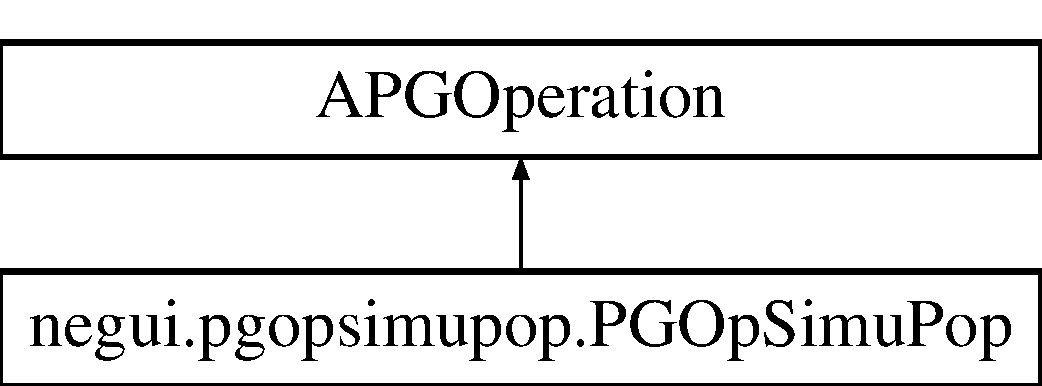
\includegraphics[height=2.000000cm]{classnegui_1_1pgopsimupop_1_1PGOpSimuPop}
\end{center}
\end{figure}
\subsection*{Public Member Functions}
\begin{DoxyCompactItemize}
\item 
def \hyperlink{classnegui_1_1pgopsimupop_1_1PGOpSimuPop_a6548b8996f7ace76266e629d9ff8c11e}{\+\_\+\+\_\+init\+\_\+\+\_\+} (self, o\+\_\+input, o\+\_\+output, b\+\_\+compress\+\_\+output=True, b\+\_\+remove\+\_\+db\+\_\+gen\+\_\+sim\+\_\+files=False, b\+\_\+write\+\_\+input\+\_\+as\+\_\+config\+\_\+file=True)
\item 
def {\bfseries prepare\+Op} (self, s\+\_\+tag\+\_\+out=\char`\"{}\char`\"{})\hypertarget{classnegui_1_1pgopsimupop_1_1PGOpSimuPop_a2f255ee2acb3d3f0341cc2f7cf1e3ad3}{}\label{classnegui_1_1pgopsimupop_1_1PGOpSimuPop_a2f255ee2acb3d3f0341cc2f7cf1e3ad3}

\item 
def {\bfseries do\+Op} (self)\hypertarget{classnegui_1_1pgopsimupop_1_1PGOpSimuPop_aed657d7d631aa0e8c2f40f8411c95dcd}{}\label{classnegui_1_1pgopsimupop_1_1PGOpSimuPop_aed657d7d631aa0e8c2f40f8411c95dcd}

\item 
def {\bfseries deliver\+Results} (self)\hypertarget{classnegui_1_1pgopsimupop_1_1PGOpSimuPop_a35c9e5794e68274f42147644b2e968c5}{}\label{classnegui_1_1pgopsimupop_1_1PGOpSimuPop_a35c9e5794e68274f42147644b2e968c5}

\end{DoxyCompactItemize}
\subsection*{Static Public Attributes}
\begin{DoxyCompactItemize}
\item 
string {\bfseries I\+N\+P\+U\+T\+\_\+\+A\+T\+T\+R\+I\+B\+U\+T\+E\+\_\+\+N\+U\+M\+B\+E\+R\+\_\+\+O\+F\+\_\+\+M\+I\+C\+R\+O\+S\+A\+TS} = \char`\"{}num\+M\+Sats\char`\"{}\hypertarget{classnegui_1_1pgopsimupop_1_1PGOpSimuPop_afad9fd5e836335f749ae96a958d3786e}{}\label{classnegui_1_1pgopsimupop_1_1PGOpSimuPop_afad9fd5e836335f749ae96a958d3786e}

\item 
string {\bfseries I\+N\+P\+U\+T\+\_\+\+A\+T\+T\+R\+I\+B\+U\+T\+E\+\_\+\+N\+U\+M\+B\+E\+R\+\_\+\+O\+F\+\_\+\+S\+N\+PS} = \char`\"{}num\+S\+N\+Ps\char`\"{}\hypertarget{classnegui_1_1pgopsimupop_1_1PGOpSimuPop_ac0c65641439fe744a0b62bd037145b3b}{}\label{classnegui_1_1pgopsimupop_1_1PGOpSimuPop_ac0c65641439fe744a0b62bd037145b3b}

\item 
string {\bfseries D\+E\+L\+I\+M\+I\+T\+E\+R\+\_\+\+I\+N\+D\+I\+V\+\_\+\+ID} = \char`\"{};\char`\"{}\hypertarget{classnegui_1_1pgopsimupop_1_1PGOpSimuPop_a23ef02f2da1b42907e37ba9d493a835a}{}\label{classnegui_1_1pgopsimupop_1_1PGOpSimuPop_a23ef02f2da1b42907e37ba9d493a835a}

\end{DoxyCompactItemize}


\subsection{Detailed Description}
\begin{DoxyVerb}This class inherits its basic interface from class APGOperation, with its 3
basic defs "prepareOp", "doOP", and "deliverResults"

Its motivating role is to be a member object of a PGGuiApp object, and to contain the
defs that do a simupop simulation and give results back to the gui.

Should use no GUI classes, but strictly utils or pop-gen calls.

This object has member two objects, an input object that fetches and prepares the
data needed for the simuPop run, and an output object that formats and/or delivers
the results.   These objects are exposed to users via getters.  The defs in these 
member objects can thus be accessed by gui widgets when an object of this class  
is used as a member of a PGGuiApp object

The functionality in the name-mangled (self.__*) defs are from Tiago Anteo's sim.py module in 
his AgeStructureNe project -- his mod-level variables simply assigned to self.
\end{DoxyVerb}
 

Definition at line 33 of file pgopsimupop.\+py.



\subsection{Constructor \& Destructor Documentation}
\index{negui\+::pgopsimupop\+::\+P\+G\+Op\+Simu\+Pop@{negui\+::pgopsimupop\+::\+P\+G\+Op\+Simu\+Pop}!\+\_\+\+\_\+init\+\_\+\+\_\+@{\+\_\+\+\_\+init\+\_\+\+\_\+}}
\index{\+\_\+\+\_\+init\+\_\+\+\_\+@{\+\_\+\+\_\+init\+\_\+\+\_\+}!negui\+::pgopsimupop\+::\+P\+G\+Op\+Simu\+Pop@{negui\+::pgopsimupop\+::\+P\+G\+Op\+Simu\+Pop}}
\subsubsection[{\texorpdfstring{\+\_\+\+\_\+init\+\_\+\+\_\+(self, o\+\_\+input, o\+\_\+output, b\+\_\+compress\+\_\+output=\+True, b\+\_\+remove\+\_\+db\+\_\+gen\+\_\+sim\+\_\+files=\+False, b\+\_\+write\+\_\+input\+\_\+as\+\_\+config\+\_\+file=\+True)}{__init__(self, o_input, o_output, b_compress_output=True, b_remove_db_gen_sim_files=False, b_write_input_as_config_file=True)}}]{\setlength{\rightskip}{0pt plus 5cm}def negui.\+pgopsimupop.\+P\+G\+Op\+Simu\+Pop.\+\_\+\+\_\+init\+\_\+\+\_\+ (
\begin{DoxyParamCaption}
\item[{}]{self, }
\item[{}]{o\+\_\+input, }
\item[{}]{o\+\_\+output, }
\item[{}]{b\+\_\+compress\+\_\+output = {\ttfamily True}, }
\item[{}]{b\+\_\+remove\+\_\+db\+\_\+gen\+\_\+sim\+\_\+files = {\ttfamily False}, }
\item[{}]{b\+\_\+write\+\_\+input\+\_\+as\+\_\+config\+\_\+file = {\ttfamily True}}
\end{DoxyParamCaption}
)}\hypertarget{classnegui_1_1pgopsimupop_1_1PGOpSimuPop_a6548b8996f7ace76266e629d9ff8c11e}{}\label{classnegui_1_1pgopsimupop_1_1PGOpSimuPop_a6548b8996f7ace76266e629d9ff8c11e}
\begin{DoxyVerb}    o_input, a PGInputSimuPop object
    o_output, a PGOutputSimuPop object
    b_compress_output, if set to True
will compress outputfiles using bz2
    b_remove_db_gen_sim_files, if set to True,
will remove the output files with the
indicated extensions.  This was added
after some testing and noting that
users most interested in using the genepop
file output suffered from the many additional
output files when trying to load genepop files
for ne-estimation
    b_write_input_as_config_file, if set to false, will 
skip the step in doOp that writes the current params
to config file, via the input objects attributes 
and defs. As for the above flag, this was added
to prevent writing identical configuration files
for replicate runs of the simulation, and thus
reduce the number of output files. \end{DoxyVerb}
 

Definition at line 59 of file pgopsimupop.\+py.


\begin{DoxyCode}
59                                     b\_write\_input\_as\_config\_file=\textcolor{keyword}{True}):  
60         \textcolor{stringliteral}{'''}
61 \textcolor{stringliteral}{            o\_input, a PGInputSimuPop object}
62 \textcolor{stringliteral}{            o\_output, a PGOutputSimuPop object}
63 \textcolor{stringliteral}{            b\_compress\_output, if set to True}
64 \textcolor{stringliteral}{                will compress outputfiles using bz2}
65 \textcolor{stringliteral}{            b\_remove\_db\_gen\_sim\_files, if set to True,}
66 \textcolor{stringliteral}{                will remove the output files with the}
67 \textcolor{stringliteral}{                indicated extensions.  This was added}
68 \textcolor{stringliteral}{                after some testing and noting that}
69 \textcolor{stringliteral}{                users most interested in using the genepop}
70 \textcolor{stringliteral}{                file output suffered from the many additional}
71 \textcolor{stringliteral}{                output files when trying to load genepop files}
72 \textcolor{stringliteral}{                for ne-estimation}
73 \textcolor{stringliteral}{            b\_write\_input\_as\_config\_file, if set to false, will }
74 \textcolor{stringliteral}{                skip the step in doOp that writes the current params}
75 \textcolor{stringliteral}{                to config file, via the input objects attributes }
76 \textcolor{stringliteral}{                and defs. As for the above flag, this was added}
77 \textcolor{stringliteral}{                to prevent writing identical configuration files}
78 \textcolor{stringliteral}{                for replicate runs of the simulation, and thus}
79 \textcolor{stringliteral}{                reduce the number of output files. }
80 \textcolor{stringliteral}{}
81 \textcolor{stringliteral}{        '''}
82 
83         super( PGOpSimuPop, self ).\hyperlink{classnegui_1_1pgopsimupop_1_1PGOpSimuPop_a6548b8996f7ace76266e629d9ff8c11e}{\_\_init\_\_}( o\_input, o\_output )
84 
85         self.\hyperlink{classnegui_1_1pgopsimupop_1_1PGOpSimuPop_a1061b53dea80371a6414760b43b2cd1e}{\_\_lSizes} = [0, 0, 0, 0, 0, 0]
86         self.\hyperlink{classnegui_1_1pgopsimupop_1_1PGOpSimuPop_a1224d81cfdf1400b2f12970074c81817}{\_\_reportOps} = [ sp.Stat(popSize=\textcolor{keyword}{True}) ]
87         self.\hyperlink{classnegui_1_1pgopsimupop_1_1PGOpSimuPop_ac10f21f990f51e85c7fab2b5aa888edd}{\_\_is\_prepared}=\textcolor{keyword}{False}
88         self.\hyperlink{classnegui_1_1pgopsimupop_1_1PGOpSimuPop_acccf36393e66057c8026cba0557d3fb8}{\_\_compress\_output}=b\_compress\_output
89         self.\hyperlink{classnegui_1_1pgopsimupop_1_1PGOpSimuPop_a5a64b272404e6113dd1c7ba70235c366}{\_\_remove\_db\_gen\_sim\_files}=b\_remove\_db\_gen\_sim\_files
90         self.\hyperlink{classnegui_1_1pgopsimupop_1_1PGOpSimuPop_a9a27655cf00df0e11603e221c314c0a9}{\_\_write\_input\_as\_config\_file}=b\_write\_input\_as\_config\_file
91 
92         \textcolor{comment}{#if this object is created in one of multiple}
93         \textcolor{comment}{#python so-called "Processes" objects from class}
94         \textcolor{comment}{#"multiprocessing", all pops in their separate "process"}
95         \textcolor{comment}{#will have identical individuals (same number/genotypes) }
96         \textcolor{comment}{#unless we reseed the numpy random number generator }
97         \textcolor{comment}{#for each "process:"}
98         numpy.random.seed()
99         
100         \textcolor{keywordflow}{return}
\end{DoxyCode}


The documentation for this class was generated from the following file\+:\begin{DoxyCompactItemize}
\item 
pgopsimupop.\+py\end{DoxyCompactItemize}

\hypertarget{classnegui_1_1pgoutputneestimator_1_1PGOutputNeEstimator}{}\section{negui.\+pgoutputneestimator.\+P\+G\+Output\+Ne\+Estimator Class Reference}
\label{classnegui_1_1pgoutputneestimator_1_1PGOutputNeEstimator}\index{negui.\+pgoutputneestimator.\+P\+G\+Output\+Ne\+Estimator@{negui.\+pgoutputneestimator.\+P\+G\+Output\+Ne\+Estimator}}
Inheritance diagram for negui.\+pgoutputneestimator.\+P\+G\+Output\+Ne\+Estimator\+:\begin{figure}[H]
\begin{center}
\leavevmode
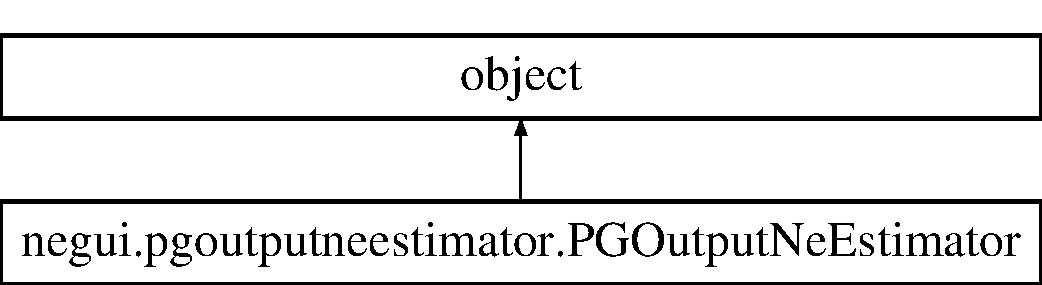
\includegraphics[height=2.000000cm]{classnegui_1_1pgoutputneestimator_1_1PGOutputNeEstimator}
\end{center}
\end{figure}
\subsection*{Public Member Functions}
\begin{DoxyCompactItemize}
\item 
def {\bfseries \+\_\+\+\_\+init\+\_\+\+\_\+} (self, s\+\_\+input\+\_\+file, s\+\_\+run\+\_\+output\+\_\+filename, o\+\_\+bias\+\_\+adjustor=None, s\+\_\+estimator\+\_\+to\+\_\+use=E\+S\+T\+I\+M\+A\+T\+O\+R\+\_\+\+N\+E\+E\+S\+T\+I\+M\+A\+T\+OR)\hypertarget{classnegui_1_1pgoutputneestimator_1_1PGOutputNeEstimator_a83a6befe7f70678330a2395b05924174}{}\label{classnegui_1_1pgoutputneestimator_1_1PGOutputNeEstimator_a83a6befe7f70678330a2395b05924174}

\item 
def \hyperlink{classnegui_1_1pgoutputneestimator_1_1PGOutputNeEstimator_a7b6885cf565cb604ab24d7082858f57b}{parse\+Output} (self)
\item 
def {\bfseries get\+No\+Dat\+File\+Name} (self)\hypertarget{classnegui_1_1pgoutputneestimator_1_1PGOutputNeEstimator_a10c975df76c0f893c4814cf0b492cae6}{}\label{classnegui_1_1pgoutputneestimator_1_1PGOutputNeEstimator_a10c975df76c0f893c4814cf0b492cae6}

\item 
def \hyperlink{classnegui_1_1pgoutputneestimator_1_1PGOutputNeEstimator_a4f8192c2aacf6e38b2c4c1d80302b643}{parse\+No\+Dat\+File} (self)
\item 
def {\bfseries get\+Column\+Number\+For\+Field\+Name} (self, s\+\_\+name)\hypertarget{classnegui_1_1pgoutputneestimator_1_1PGOutputNeEstimator_a9f13fc3000c3018a20fb38f37c5d9594}{}\label{classnegui_1_1pgoutputneestimator_1_1PGOutputNeEstimator_a9f13fc3000c3018a20fb38f37c5d9594}

\item 
def {\bfseries parsed\+\_\+output} (self)\hypertarget{classnegui_1_1pgoutputneestimator_1_1PGOutputNeEstimator_ae97f8f35f02d9026bc1796daa3ed7aca}{}\label{classnegui_1_1pgoutputneestimator_1_1PGOutputNeEstimator_ae97f8f35f02d9026bc1796daa3ed7aca}

\item 
def {\bfseries parsed\+\_\+nodat\+\_\+info} (self)\hypertarget{classnegui_1_1pgoutputneestimator_1_1PGOutputNeEstimator_a9842661b1a2ff8f5b0fb95cdbf45c1f9}{}\label{classnegui_1_1pgoutputneestimator_1_1PGOutputNeEstimator_a9842661b1a2ff8f5b0fb95cdbf45c1f9}

\item 
def {\bfseries run\+\_\+output\+\_\+file} (self)\hypertarget{classnegui_1_1pgoutputneestimator_1_1PGOutputNeEstimator_a5e510dccae0f66ae63f86d46e6c46a36}{}\label{classnegui_1_1pgoutputneestimator_1_1PGOutputNeEstimator_a5e510dccae0f66ae63f86d46e6c46a36}

\item 
def {\bfseries output\+\_\+file} (self, s\+\_\+name)\hypertarget{classnegui_1_1pgoutputneestimator_1_1PGOutputNeEstimator_a67501f770ac63303d0ed3b69fc148544}{}\label{classnegui_1_1pgoutputneestimator_1_1PGOutputNeEstimator_a67501f770ac63303d0ed3b69fc148544}

\item 
def {\bfseries run\+\_\+input\+\_\+file} (self)\hypertarget{classnegui_1_1pgoutputneestimator_1_1PGOutputNeEstimator_ac3204c39eb40e0e5a9c16906382d98a5}{}\label{classnegui_1_1pgoutputneestimator_1_1PGOutputNeEstimator_ac3204c39eb40e0e5a9c16906382d98a5}

\item 
def {\bfseries run\+\_\+input\+\_\+file} (self, s\+\_\+name)\hypertarget{classnegui_1_1pgoutputneestimator_1_1PGOutputNeEstimator_aaa66e700b71e0f86af69c9301be4aed2}{}\label{classnegui_1_1pgoutputneestimator_1_1PGOutputNeEstimator_aaa66e700b71e0f86af69c9301be4aed2}

\item 
def {\bfseries output\+\_\+fields} (self)\hypertarget{classnegui_1_1pgoutputneestimator_1_1PGOutputNeEstimator_a3c833e27a8bf526b8e0003843d21f7aa}{}\label{classnegui_1_1pgoutputneestimator_1_1PGOutputNeEstimator_a3c833e27a8bf526b8e0003843d21f7aa}

\end{DoxyCompactItemize}
\subsection*{Static Public Attributes}
\begin{DoxyCompactItemize}
\item 
list {\bfseries O\+U\+T\+P\+U\+T\+\_\+\+F\+I\+E\+L\+DS}
\item 
list {\bfseries N\+O\+D\+A\+T\+\_\+\+F\+I\+E\+L\+DS} = \mbox{[} \char`\"{}Individual\char`\"{}, \char`\"{}Locus\char`\"{}, \char`\"{}Genotype\char`\"{}, \char`\"{}Number\+Loci\+Missing\+Data\char`\"{} \mbox{]}\hypertarget{classnegui_1_1pgoutputneestimator_1_1PGOutputNeEstimator_a4e5c6c9926a8f963e36d83d858366c4d}{}\label{classnegui_1_1pgoutputneestimator_1_1PGOutputNeEstimator_a4e5c6c9926a8f963e36d83d858366c4d}

\item 
list {\bfseries O\+U\+T\+P\+U\+T\+\_\+\+T\+I\+A\+G\+O\+\_\+\+A\+B\+B\+R\+E\+VS} = \mbox{[} \char`\"{}ne\char`\"{},\char`\"{}neci05\char`\"{} , \char`\"{}neci975\char`\"{}, \char`\"{}or2\char`\"{}, \char`\"{}sr2\char`\"{}, \char`\"{}indep\char`\"{}, \char`\"{}hmean\char`\"{} \mbox{]}\hypertarget{classnegui_1_1pgoutputneestimator_1_1PGOutputNeEstimator_a916a47666e6360ea279b944832907b27}{}\label{classnegui_1_1pgoutputneestimator_1_1PGOutputNeEstimator_a916a47666e6360ea279b944832907b27}

\end{DoxyCompactItemize}


\subsection{Detailed Description}
\begin{DoxyVerb}Object manages output from the PGOpNeEstimator object
\end{DoxyVerb}
 

Definition at line 42 of file pgoutputneestimator.\+py.



\subsection{Member Function Documentation}
\index{negui\+::pgoutputneestimator\+::\+P\+G\+Output\+Ne\+Estimator@{negui\+::pgoutputneestimator\+::\+P\+G\+Output\+Ne\+Estimator}!parse\+No\+Dat\+File@{parse\+No\+Dat\+File}}
\index{parse\+No\+Dat\+File@{parse\+No\+Dat\+File}!negui\+::pgoutputneestimator\+::\+P\+G\+Output\+Ne\+Estimator@{negui\+::pgoutputneestimator\+::\+P\+G\+Output\+Ne\+Estimator}}
\subsubsection[{\texorpdfstring{parse\+No\+Dat\+File(self)}{parseNoDatFile(self)}}]{\setlength{\rightskip}{0pt plus 5cm}def negui.\+pgoutputneestimator.\+P\+G\+Output\+Ne\+Estimator.\+parse\+No\+Dat\+File (
\begin{DoxyParamCaption}
\item[{}]{self}
\end{DoxyParamCaption}
)}\hypertarget{classnegui_1_1pgoutputneestimator_1_1PGOutputNeEstimator_a4f8192c2aacf6e38b2c4c1d80302b643}{}\label{classnegui_1_1pgoutputneestimator_1_1PGOutputNeEstimator_a4f8192c2aacf6e38b2c4c1d80302b643}
\begin{DoxyVerb}This def is provisional, since I have only seen
a few of the *NoDat.txt files generated by
NeEstimator (v2). I base the parsing on examples like this:

Population 1 [OmyLGRA12S_0213]  
-----------------------------------------------------------
Individual       Locus         Genotype     Number of Loci
                          with missing data
       1            9             0000             4   
----------------------------------------------------------  

    

However thin the ground, this def assumes

1. multipop results will simply have more table entries
like the one above.

2. If a line in the NeEstimator's "*NoDat.txt" file
starts with the value below in COLHEADSTART, and 
contains the other column keywords given below
in COLSINCLUDE, that is must be the header and
also that the data follows after one mostly line blank
but for a tag on the last column header

3. Population name entry for each table is uniqely
located by the line starting with value below in POPLINESTART
\end{DoxyVerb}
 

Definition at line 383 of file pgoutputneestimator.\+py.


\begin{DoxyCode}
383     \textcolor{keyword}{def }\hyperlink{classnegui_1_1pgoutputneestimator_1_1PGOutputNeEstimator_a4f8192c2aacf6e38b2c4c1d80302b643}{parseNoDatFile}( self ):
384         \textcolor{stringliteral}{'''}
385 \textcolor{stringliteral}{        This def is provisional, since I have only seen}
386 \textcolor{stringliteral}{        a few of the *NoDat.txt files generated by}
387 \textcolor{stringliteral}{        NeEstimator (v2). I base the parsing on examples like this:}
388 \textcolor{stringliteral}{}
389 \textcolor{stringliteral}{        Population 1 [OmyLGRA12S\_0213]  }
390 \textcolor{stringliteral}{        -----------------------------------------------------------}
391 \textcolor{stringliteral}{        Individual       Locus         Genotype     Number of Loci}
392 \textcolor{stringliteral}{                                          with missing data}
393 \textcolor{stringliteral}{               1            9             0000             4   }
394 \textcolor{stringliteral}{        ----------------------------------------------------------  }
395 \textcolor{stringliteral}{        }
396 \textcolor{stringliteral}{    }
397 \textcolor{stringliteral}{        }
398 \textcolor{stringliteral}{        However thin the ground, this def assumes}
399 \textcolor{stringliteral}{}
400 \textcolor{stringliteral}{        1. multipop results will simply have more table entries}
401 \textcolor{stringliteral}{        like the one above.}
402 \textcolor{stringliteral}{}
403 \textcolor{stringliteral}{        2. If a line in the NeEstimator's "*NoDat.txt" file}
404 \textcolor{stringliteral}{        starts with the value below in COLHEADSTART, and }
405 \textcolor{stringliteral}{        contains the other column keywords given below}
406 \textcolor{stringliteral}{        in COLSINCLUDE, that is must be the header and}
407 \textcolor{stringliteral}{        also that the data follows after one mostly line blank}
408 \textcolor{stringliteral}{        but for a tag on the last column header}
409 \textcolor{stringliteral}{}
410 \textcolor{stringliteral}{        3. Population name entry for each table is uniqely}
411 \textcolor{stringliteral}{        located by the line starting with value below in POPLINESTART}
412 \textcolor{stringliteral}{        '''}
413 
414 
415         POPLINESTART=\textcolor{stringliteral}{"Population"}
416         COLHEADSTART=\textcolor{stringliteral}{"Individual"}       
417         COLSINCLUDE=[ \textcolor{stringliteral}{"Locus"}, \textcolor{stringliteral}{"Genotype"}, \textcolor{stringliteral}{"Number of Loci"} ]
418         ENDTABLELINESTART=\textcolor{stringliteral}{"----------------------"}  
419 
420         s\_name=self.\hyperlink{classnegui_1_1pgoutputneestimator_1_1PGOutputNeEstimator_ab1fea13d322982ecc8b5fbe42741de50}{\_\_get\_name\_nodat\_file}()
421 
422         \textcolor{keywordflow}{if} s\_name \textcolor{keywordflow}{is} \textcolor{keywordtype}{None}:
423             \textcolor{keywordflow}{return}
424         \textcolor{comment}{#end return if no nodat file}
425 
426         self.\hyperlink{classnegui_1_1pgoutputneestimator_1_1PGOutputNeEstimator_acd31d6f910fc03d1945e38b6c4fa79c0}{\_\_parsed\_nodat\_output}=[]
427 
428         o\_file=open( s\_name )
429 
430         b\_found\_header=\textcolor{keyword}{False}
431         i\_table\_lines\_count=0
432         s\_currpop=\textcolor{stringliteral}{""}
433         \textcolor{keywordflow}{for} s\_line \textcolor{keywordflow}{in} o\_file:
434 
435             i\_num\_match=0
436             \textcolor{keywordflow}{if} s\_line.startswith( POPLINESTART ):
437                 \textcolor{comment}{#we replace spaces in the pop name:}
438                 s\_currpop=s\_line.strip().replace( \textcolor{stringliteral}{" "}, \textcolor{stringliteral}{"\_"} )
439             \textcolor{keywordflow}{elif} s\_line.startswith(COLHEADSTART):
440                 lb\_trues=[ s\_col \textcolor{keywordflow}{in} s\_line \textcolor{keywordflow}{for} s\_col \textcolor{keywordflow}{in} COLSINCLUDE ]
441                 \textcolor{keywordflow}{if} sum( lb\_trues ) == len( COLSINCLUDE ):
442                     b\_found\_header=\textcolor{keyword}{True}
443                     i\_table\_lines\_count=0
444                 \textcolor{comment}{#end if all header names in line}
445             \textcolor{keywordflow}{else}:
446                 \textcolor{comment}{#first line after header is more header:}
447                 \textcolor{keywordflow}{if} b\_found\_header \textcolor{keywordflow}{and} i\_table\_lines\_count > 1:
448                     \textcolor{comment}{#if end of table for currpop, }
449                     \textcolor{comment}{#reset flag, line counts}
450                     \textcolor{keywordflow}{if} s\_line.startswith( ENDTABLELINESTART ):
451                         b\_found\_header=\textcolor{keyword}{False}
452                         i\_table\_lines\_count=0
453                     \textcolor{keywordflow}{else}:
454                         i\_table\_lines\_count+=1
455                         \textcolor{comment}{#NoDat.txt files data cols}
456                         \textcolor{comment}{#are seperated by multiple space chars,}
457                         \textcolor{comment}{#so we use the default split to}
458                         \textcolor{comment}{#list only non-space as items:  }
459                         ls\_vals=s\_line.strip().split() 
460                         \textcolor{comment}{#first col is the pop name}
461                         self.\_\_parsed\_nodat\_output.append( [ s\_currpop ] \(\backslash\)
462                                 + [ s\_val \textcolor{keywordflow}{for} s\_val \textcolor{keywordflow}{in} ls\_vals ] )
463                     \textcolor{comment}{#end if end-table line, else data}
464                 \textcolor{comment}{#end if header's been found and we're past the non-date line}
465             \textcolor{comment}{#end if pop line else header line, else some other line}
466         \textcolor{comment}{#end for each line in nodat file}
467 
468         o\_file.close()
469         \textcolor{keywordflow}{return}
\end{DoxyCode}
\index{negui\+::pgoutputneestimator\+::\+P\+G\+Output\+Ne\+Estimator@{negui\+::pgoutputneestimator\+::\+P\+G\+Output\+Ne\+Estimator}!parse\+Output@{parse\+Output}}
\index{parse\+Output@{parse\+Output}!negui\+::pgoutputneestimator\+::\+P\+G\+Output\+Ne\+Estimator@{negui\+::pgoutputneestimator\+::\+P\+G\+Output\+Ne\+Estimator}}
\subsubsection[{\texorpdfstring{parse\+Output(self)}{parseOutput(self)}}]{\setlength{\rightskip}{0pt plus 5cm}def negui.\+pgoutputneestimator.\+P\+G\+Output\+Ne\+Estimator.\+parse\+Output (
\begin{DoxyParamCaption}
\item[{}]{self}
\end{DoxyParamCaption}
)}\hypertarget{classnegui_1_1pgoutputneestimator_1_1PGOutputNeEstimator_a7b6885cf565cb604ab24d7082858f57b}{}\label{classnegui_1_1pgoutputneestimator_1_1PGOutputNeEstimator_a7b6885cf565cb604ab24d7082858f57b}
\begin{DoxyVerb}Fri Jul 22 18:07:53 MDT 2016 -- See 
def __ne2_record_object_to_dictionary for details on the
ddv_results fetched below to unwrap the parsed results,
and the current limitation to estimation type LD

We assume that for the estimated ne value,
and its associated CI values, that a value of None in
the dict returned by ne2.parse def (see above 
__get_parsed_output_data, reflects
an "Infinite" value in the origina Ne estimator output
and so convert it to "Inf,"  convenient for use in R,
for example, as R uses Inf for Infinity

2017_03_20.  We revise this def to allow getting parsed 
data from an LDNe2 run, rather than an NeEstimator run. We 
move the original code that is processing the ne estimator
data as retrived using pygenomics.genomics.popgen.ne code,
to a new def specified for the ne-estimator, 
__set_parsed_output_using_ne_estimator_data.
This also involves renaming some existing defs, for example:
    __get_parsed_output_data -> __get_ne_estimator_parsed_output_data
\end{DoxyVerb}
 

Definition at line 255 of file pgoutputneestimator.\+py.


\begin{DoxyCode}
255     \textcolor{keyword}{def }\hyperlink{classnegui_1_1pgoutputneestimator_1_1PGOutputNeEstimator_a7b6885cf565cb604ab24d7082858f57b}{parseOutput}( self ):
256         \textcolor{stringliteral}{'''}
257 \textcolor{stringliteral}{        Fri Jul 22 18:07:53 MDT 2016 -- See }
258 \textcolor{stringliteral}{        def \_\_ne2\_record\_object\_to\_dictionary for details on the}
259 \textcolor{stringliteral}{        ddv\_results fetched below to unwrap the parsed results,}
260 \textcolor{stringliteral}{        and the current limitation to estimation type LD}
261 \textcolor{stringliteral}{}
262 \textcolor{stringliteral}{        We assume that for the estimated ne value,}
263 \textcolor{stringliteral}{        and its associated CI values, that a value of None in}
264 \textcolor{stringliteral}{        the dict returned by ne2.parse def (see above }
265 \textcolor{stringliteral}{        \_\_get\_parsed\_output\_data, reflects}
266 \textcolor{stringliteral}{        an "Infinite" value in the origina Ne estimator output}
267 \textcolor{stringliteral}{        and so convert it to "Inf,"  convenient for use in R,}
268 \textcolor{stringliteral}{        for example, as R uses Inf for Infinity}
269 \textcolor{stringliteral}{        }
270 \textcolor{stringliteral}{        2017\_03\_20.  We revise this def to allow getting parsed }
271 \textcolor{stringliteral}{        data from an LDNe2 run, rather than an NeEstimator run. We }
272 \textcolor{stringliteral}{        move the original code that is processing the ne estimator}
273 \textcolor{stringliteral}{        data as retrived using pygenomics.genomics.popgen.ne code,}
274 \textcolor{stringliteral}{        to a new def specified for the ne-estimator, }
275 \textcolor{stringliteral}{        \_\_set\_parsed\_output\_using\_ne\_estimator\_data.}
276 \textcolor{stringliteral}{        This also involves renaming some existing defs, for example:}
277 \textcolor{stringliteral}{            \_\_get\_parsed\_output\_data -> \_\_get\_ne\_estimator\_parsed\_output\_data}
278 \textcolor{stringliteral}{        '''}
279         \textcolor{keywordflow}{if} self.\hyperlink{classnegui_1_1pgoutputneestimator_1_1PGOutputNeEstimator_a4d34bdc2e4c4fdc788722b016348c6ee}{\_\_estimator}==ESTIMATOR\_NEESTIMATOR:
280             self.\hyperlink{classnegui_1_1pgoutputneestimator_1_1PGOutputNeEstimator_a10df28bc24347e441b225c3e5a7f3630}{\_\_set\_parsed\_output\_attribute\_using\_ne\_estimator\_data}
      ()
281         \textcolor{keywordflow}{elif} self.\hyperlink{classnegui_1_1pgoutputneestimator_1_1PGOutputNeEstimator_a4d34bdc2e4c4fdc788722b016348c6ee}{\_\_estimator}==ESTIMATOR\_LDNE:
282             self.\hyperlink{classnegui_1_1pgoutputneestimator_1_1PGOutputNeEstimator_ab60141608f13bb990250641db8b3817c}{\_\_set\_parsed\_output\_attribute\_using\_ldne\_data}
      ()
283         \textcolor{keywordflow}{else}:
284             s\_msg=\textcolor{stringliteral}{"In PGOutputNeEstimator instance, def parseOutput, "} \(\backslash\)
285                             + \textcolor{stringliteral}{"The estimator program name is unknown: "} \(\backslash\)
286                             + self.\hyperlink{classnegui_1_1pgoutputneestimator_1_1PGOutputNeEstimator_a4d34bdc2e4c4fdc788722b016348c6ee}{\_\_estimator}
287             \textcolor{keywordflow}{raise} Exception( s\_msg )
288         \textcolor{comment}{#end if neestimator, else ldne}
289         \textcolor{keywordflow}{return}
\end{DoxyCode}


\subsection{Member Data Documentation}
\index{negui\+::pgoutputneestimator\+::\+P\+G\+Output\+Ne\+Estimator@{negui\+::pgoutputneestimator\+::\+P\+G\+Output\+Ne\+Estimator}!O\+U\+T\+P\+U\+T\+\_\+\+F\+I\+E\+L\+DS@{O\+U\+T\+P\+U\+T\+\_\+\+F\+I\+E\+L\+DS}}
\index{O\+U\+T\+P\+U\+T\+\_\+\+F\+I\+E\+L\+DS@{O\+U\+T\+P\+U\+T\+\_\+\+F\+I\+E\+L\+DS}!negui\+::pgoutputneestimator\+::\+P\+G\+Output\+Ne\+Estimator@{negui\+::pgoutputneestimator\+::\+P\+G\+Output\+Ne\+Estimator}}
\subsubsection[{\texorpdfstring{O\+U\+T\+P\+U\+T\+\_\+\+F\+I\+E\+L\+DS}{OUTPUT_FIELDS}}]{\setlength{\rightskip}{0pt plus 5cm}list negui.\+pgoutputneestimator.\+P\+G\+Output\+Ne\+Estimator.\+O\+U\+T\+P\+U\+T\+\_\+\+F\+I\+E\+L\+DS\hspace{0.3cm}{\ttfamily [static]}}\hypertarget{classnegui_1_1pgoutputneestimator_1_1PGOutputNeEstimator_aa78fb93f7acf4a769ae309f1a3b94302}{}\label{classnegui_1_1pgoutputneestimator_1_1PGOutputNeEstimator_aa78fb93f7acf4a769ae309f1a3b94302}
{\bfseries Initial value\+:}
\begin{DoxyCode}
1 = [ \textcolor{stringliteral}{"est\_type"}, \textcolor{stringliteral}{"case\_number"}, \textcolor{stringliteral}{"est\_ne"},\textcolor{stringliteral}{"95ci\_low"},\textcolor{stringliteral}{"95ci\_high"}, \textcolor{stringliteral}{"overall\_rsquared"},
2                     \textcolor{stringliteral}{"expected\_rsquared"},\textcolor{stringliteral}{"indep\_comparisons"},\textcolor{stringliteral}{"harmon\_mean\_samp\_size"}, \textcolor{stringliteral}{"alt\_ci\_low"}, \textcolor{stringliteral}{"
      alt\_ci\_high"} ]
\end{DoxyCode}


Definition at line 48 of file pgoutputneestimator.\+py.



The documentation for this class was generated from the following file\+:\begin{DoxyCompactItemize}
\item 
pgoutputneestimator.\+py\end{DoxyCompactItemize}

\hypertarget{classnegui_1_1pgoutputsimupop_1_1PGOutputSimuPop}{}\section{negui.\+pgoutputsimupop.\+P\+G\+Output\+Simu\+Pop Class Reference}
\label{classnegui_1_1pgoutputsimupop_1_1PGOutputSimuPop}\index{negui.\+pgoutputsimupop.\+P\+G\+Output\+Simu\+Pop@{negui.\+pgoutputsimupop.\+P\+G\+Output\+Simu\+Pop}}
Inheritance diagram for negui.\+pgoutputsimupop.\+P\+G\+Output\+Simu\+Pop\+:\begin{figure}[H]
\begin{center}
\leavevmode
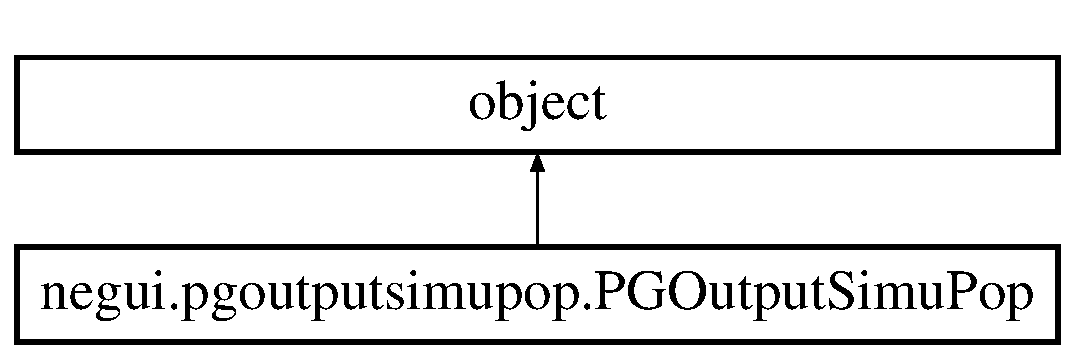
\includegraphics[height=2.000000cm]{classnegui_1_1pgoutputsimupop_1_1PGOutputSimuPop}
\end{center}
\end{figure}
\subsection*{Public Member Functions}
\begin{DoxyCompactItemize}
\item 
def {\bfseries \+\_\+\+\_\+init\+\_\+\+\_\+} (self, s\+\_\+output\+\_\+files\+\_\+prefix)\hypertarget{classnegui_1_1pgoutputsimupop_1_1PGOutputSimuPop_a8f42fc0afc9024177960bb6287e45493}{}\label{classnegui_1_1pgoutputsimupop_1_1PGOutputSimuPop_a8f42fc0afc9024177960bb6287e45493}

\item 
def {\bfseries open\+Out} (self)\hypertarget{classnegui_1_1pgoutputsimupop_1_1PGOutputSimuPop_a7cea46f9212d05e98ce14b7647781590}{}\label{classnegui_1_1pgoutputsimupop_1_1PGOutputSimuPop_a7cea46f9212d05e98ce14b7647781590}

\item 
def {\bfseries open\+Err} (self)\hypertarget{classnegui_1_1pgoutputsimupop_1_1PGOutputSimuPop_ae3f0c28a1a9afbef82fddd8d26d3ea3b}{}\label{classnegui_1_1pgoutputsimupop_1_1PGOutputSimuPop_ae3f0c28a1a9afbef82fddd8d26d3ea3b}

\item 
def {\bfseries open\+Mega\+DB} (self)\hypertarget{classnegui_1_1pgoutputsimupop_1_1PGOutputSimuPop_afac367cb22b4498a2c5170173de1bdc1}{}\label{classnegui_1_1pgoutputsimupop_1_1PGOutputSimuPop_afac367cb22b4498a2c5170173de1bdc1}

\item 
def {\bfseries copy\+Me} (self)\hypertarget{classnegui_1_1pgoutputsimupop_1_1PGOutputSimuPop_a5ab021b0ff9d452891a52313b9402fbf}{}\label{classnegui_1_1pgoutputsimupop_1_1PGOutputSimuPop_a5ab021b0ff9d452891a52313b9402fbf}

\item 
def {\bfseries open\+Conf} (self)\hypertarget{classnegui_1_1pgoutputsimupop_1_1PGOutputSimuPop_abd8a699e5a3adf2b746bdb778602fe60}{}\label{classnegui_1_1pgoutputsimupop_1_1PGOutputSimuPop_abd8a699e5a3adf2b746bdb778602fe60}

\item 
def \hyperlink{classnegui_1_1pgoutputsimupop_1_1PGOutputSimuPop_a3046e1eac1fbd82acf47c0f7c0d06b70}{bz2\+Compress\+All\+Files} (self, ls\+\_\+files\+\_\+to\+\_\+skip=\mbox{[}$\,$\mbox{]})
\item 
def \hyperlink{classnegui_1_1pgoutputsimupop_1_1PGOutputSimuPop_af093f63ef577cb9d9778920ec6589516}{gen2\+Genepop} (self, idx\+\_\+allele\+\_\+start, idx\+\_\+allele\+\_\+stop, b\+\_\+do\+\_\+compress=True, b\+\_\+pop\+\_\+per\+\_\+gen=False)
\item 
def {\bfseries remove\+Output\+File\+By\+Ext} (self, s\+\_\+extension)\hypertarget{classnegui_1_1pgoutputsimupop_1_1PGOutputSimuPop_a27af4e615fcb17d2343dc27f614c1359}{}\label{classnegui_1_1pgoutputsimupop_1_1PGOutputSimuPop_a27af4e615fcb17d2343dc27f614c1359}

\item 
def {\bfseries basename} (self)\hypertarget{classnegui_1_1pgoutputsimupop_1_1PGOutputSimuPop_af67ba734fbe5d4240a8cef38e63586d1}{}\label{classnegui_1_1pgoutputsimupop_1_1PGOutputSimuPop_af67ba734fbe5d4240a8cef38e63586d1}

\item 
def {\bfseries basename} (self, s\+\_\+basename)\hypertarget{classnegui_1_1pgoutputsimupop_1_1PGOutputSimuPop_aafca25668d51a1beec732306b7973884}{}\label{classnegui_1_1pgoutputsimupop_1_1PGOutputSimuPop_aafca25668d51a1beec732306b7973884}

\item 
def {\bfseries confname} (self)\hypertarget{classnegui_1_1pgoutputsimupop_1_1PGOutputSimuPop_a67795b5f8245e4e921615ac4cc79a5be}{}\label{classnegui_1_1pgoutputsimupop_1_1PGOutputSimuPop_a67795b5f8245e4e921615ac4cc79a5be}

\item 
def {\bfseries simname} (self)\hypertarget{classnegui_1_1pgoutputsimupop_1_1PGOutputSimuPop_ac3e82333b61e2c3e9545c9ca8e9cf64c}{}\label{classnegui_1_1pgoutputsimupop_1_1PGOutputSimuPop_ac3e82333b61e2c3e9545c9ca8e9cf64c}

\item 
def {\bfseries genname} (self)\hypertarget{classnegui_1_1pgoutputsimupop_1_1PGOutputSimuPop_a43b4446563d323091900f8b6bcfd6044}{}\label{classnegui_1_1pgoutputsimupop_1_1PGOutputSimuPop_a43b4446563d323091900f8b6bcfd6044}

\item 
def {\bfseries dbname} (self)\hypertarget{classnegui_1_1pgoutputsimupop_1_1PGOutputSimuPop_a6159d8c414cea2420a3de80ab00222bc}{}\label{classnegui_1_1pgoutputsimupop_1_1PGOutputSimuPop_a6159d8c414cea2420a3de80ab00222bc}

\end{DoxyCompactItemize}
\subsection*{Public Attributes}
\begin{DoxyCompactItemize}
\item 
{\bfseries out}\hypertarget{classnegui_1_1pgoutputsimupop_1_1PGOutputSimuPop_a4198008f7f7f029a29f8441ea7619170}{}\label{classnegui_1_1pgoutputsimupop_1_1PGOutputSimuPop_a4198008f7f7f029a29f8441ea7619170}

\item 
{\bfseries err}\hypertarget{classnegui_1_1pgoutputsimupop_1_1PGOutputSimuPop_a5eeccbf099cd8be3e8ab5906565d7b79}{}\label{classnegui_1_1pgoutputsimupop_1_1PGOutputSimuPop_a5eeccbf099cd8be3e8ab5906565d7b79}

\item 
{\bfseries mega\+DB}\hypertarget{classnegui_1_1pgoutputsimupop_1_1PGOutputSimuPop_a76379971c8aa1a3b175f171821b0b8f1}{}\label{classnegui_1_1pgoutputsimupop_1_1PGOutputSimuPop_a76379971c8aa1a3b175f171821b0b8f1}

\item 
{\bfseries conf}\hypertarget{classnegui_1_1pgoutputsimupop_1_1PGOutputSimuPop_ac6e385cca72ff0073251b511eea1103f}{}\label{classnegui_1_1pgoutputsimupop_1_1PGOutputSimuPop_ac6e385cca72ff0073251b511eea1103f}

\end{DoxyCompactItemize}
\subsection*{Static Public Attributes}
\begin{DoxyCompactItemize}
\item 
dictionary {\bfseries D\+I\+C\+T\+\_\+\+O\+U\+T\+P\+U\+T\+\_\+\+F\+I\+L\+E\+\_\+\+E\+X\+T\+E\+N\+S\+I\+O\+NS}
\item 
string {\bfseries C\+O\+M\+P\+R\+E\+S\+S\+I\+O\+N\+\_\+\+F\+I\+L\+E\+\_\+\+E\+X\+T\+E\+N\+S\+I\+ON} = \char`\"{}bz2\char`\"{}\hypertarget{classnegui_1_1pgoutputsimupop_1_1PGOutputSimuPop_aaf295d98adb01d86781790b5a57c5348}{}\label{classnegui_1_1pgoutputsimupop_1_1PGOutputSimuPop_aaf295d98adb01d86781790b5a57c5348}

\end{DoxyCompactItemize}


\subsection{Detailed Description}
\begin{DoxyVerb}Object meant to fetch parameter values and prepare them for 
use in a simuPop simulation.  

Object to be passed to a PGOpSimuPop object, which is, in turn,
passed to a PGGuiSimuPop object, so that the widgets can then access
defs in this input object, in order to, for example, show or allow
changes in parameter values for users before they run the simulation.
\end{DoxyVerb}
 

Definition at line 25 of file pgoutputsimupop.\+py.



\subsection{Member Function Documentation}
\index{negui\+::pgoutputsimupop\+::\+P\+G\+Output\+Simu\+Pop@{negui\+::pgoutputsimupop\+::\+P\+G\+Output\+Simu\+Pop}!bz2\+Compress\+All\+Files@{bz2\+Compress\+All\+Files}}
\index{bz2\+Compress\+All\+Files@{bz2\+Compress\+All\+Files}!negui\+::pgoutputsimupop\+::\+P\+G\+Output\+Simu\+Pop@{negui\+::pgoutputsimupop\+::\+P\+G\+Output\+Simu\+Pop}}
\subsubsection[{\texorpdfstring{bz2\+Compress\+All\+Files(self, ls\+\_\+files\+\_\+to\+\_\+skip=[])}{bz2CompressAllFiles(self, ls_files_to_skip=[])}}]{\setlength{\rightskip}{0pt plus 5cm}def negui.\+pgoutputsimupop.\+P\+G\+Output\+Simu\+Pop.\+bz2\+Compress\+All\+Files (
\begin{DoxyParamCaption}
\item[{}]{self, }
\item[{}]{ls\+\_\+files\+\_\+to\+\_\+skip = {\ttfamily \mbox{[}\mbox{]}}}
\end{DoxyParamCaption}
)}\hypertarget{classnegui_1_1pgoutputsimupop_1_1PGOutputSimuPop_a3046e1eac1fbd82acf47c0f7c0d06b70}{}\label{classnegui_1_1pgoutputsimupop_1_1PGOutputSimuPop_a3046e1eac1fbd82acf47c0f7c0d06b70}
\begin{DoxyVerb}used code and advice in, 
http://stackoverflow.com/questions/9518705/big-file-compression-with-python

Note: checked the shutil documentation at https://docs.python.org/2/library/shutil.html
which warns of loss of meta file info (owner/group ACLs) when using shutil.copy() or shutil.copy2().  Unclear
whether this applies to the copyfileobj, though my few tests showd all of these were retained.
\end{DoxyVerb}
 

Definition at line 168 of file pgoutputsimupop.\+py.


\begin{DoxyCode}
168     \textcolor{keyword}{def }\hyperlink{classnegui_1_1pgoutputsimupop_1_1PGOutputSimuPop_a3046e1eac1fbd82acf47c0f7c0d06b70}{bz2CompressAllFiles}(self, ls\_files\_to\_skip=[] ):
169         \textcolor{stringliteral}{'''}
170 \textcolor{stringliteral}{        used code and advice in, }
171 \textcolor{stringliteral}{        http://stackoverflow.com/questions/9518705/big-file-compression-with-python}
172 \textcolor{stringliteral}{}
173 \textcolor{stringliteral}{        Note: checked the shutil documentation at https://docs.python.org/2/library/shutil.html}
174 \textcolor{stringliteral}{        which warns of loss of meta file info (owner/group ACLs) when using shutil.copy() or
       shutil.copy2().  Unclear}
175 \textcolor{stringliteral}{        whether this applies to the copyfileobj, though my few tests showd all of these were retained.}
176 \textcolor{stringliteral}{        '''}
177         \textcolor{keywordflow}{for} s\_myfile \textcolor{keywordflow}{in} [ self.\hyperlink{classnegui_1_1pgoutputsimupop_1_1PGOutputSimuPop_a50f64be6bb990a0ac6898a44b4bf6fbc}{\_\_outname}, self.\hyperlink{classnegui_1_1pgoutputsimupop_1_1PGOutputSimuPop_a26363a7bbc4ae53b86585e32f0360e2a}{\_\_errname}, self.
      \hyperlink{classnegui_1_1pgoutputsimupop_1_1PGOutputSimuPop_aa89de70104807ce7e26bb17310f74b97}{\_\_megadbname}, self.\hyperlink{classnegui_1_1pgoutputsimupop_1_1PGOutputSimuPop_af5c9a72247505d2c2bb3d7400cbc09b3}{\_\_confname} ]:
178             
179             \textcolor{keywordflow}{if} s\_myfile \textcolor{keywordflow}{in} ls\_files\_to\_skip:
180                 \textcolor{keywordflow}{pass}
181             \textcolor{keywordflow}{elif} \textcolor{keywordflow}{not} self.\hyperlink{classnegui_1_1pgoutputsimupop_1_1PGOutputSimuPop_a1fdfb988619bd4a9d377a1e20f52839c}{\_\_file\_exists}( s\_myfile ):
182                 self.\hyperlink{classnegui_1_1pgoutputsimupop_1_1PGOutputSimuPop_abf6aab4f7982c2b0f9e4544343bf241b}{\_\_raise\_file\_not\_found\_error}( s\_myfile, \textcolor{stringliteral}{"compress file
       with bz2"}  )
183             \textcolor{keywordflow}{else}:
184                 with open( s\_myfile, \textcolor{stringliteral}{'rb'} ) \textcolor{keyword}{as} o\_input:
185                     with bz2.BZ2File( s\_myfile + \textcolor{stringliteral}{'.bz2'}, \textcolor{stringliteral}{'wb'}, compresslevel=9 ) \textcolor{keyword}{as} o\_output:
186                         \textcolor{comment}{#try/except overkill, but want logic to show}
187                         \textcolor{comment}{#we don't remove the input file}
188                         \textcolor{comment}{#if the copy op fails:}
189                         \textcolor{keywordflow}{try}: 
190                             shutil.copyfileobj( o\_input, o\_output )
191                         \textcolor{keywordflow}{except} Exception,  e:
192                             \textcolor{keywordflow}{raise} e
193                         \textcolor{comment}{#end try except}
194 
195                         \textcolor{comment}{#required by windows only, else error can't remove:}
196                         o\_input.close()
197                         os.remove( s\_myfile )   
198                     \textcolor{comment}{#end with bzfile for writing}
199                 \textcolor{comment}{#end with current file for reading}
200             \textcolor{comment}{#end if file absent, else exists}
201         \textcolor{comment}{#end for each file}
\end{DoxyCode}
\index{negui\+::pgoutputsimupop\+::\+P\+G\+Output\+Simu\+Pop@{negui\+::pgoutputsimupop\+::\+P\+G\+Output\+Simu\+Pop}!gen2\+Genepop@{gen2\+Genepop}}
\index{gen2\+Genepop@{gen2\+Genepop}!negui\+::pgoutputsimupop\+::\+P\+G\+Output\+Simu\+Pop@{negui\+::pgoutputsimupop\+::\+P\+G\+Output\+Simu\+Pop}}
\subsubsection[{\texorpdfstring{gen2\+Genepop(self, idx\+\_\+allele\+\_\+start, idx\+\_\+allele\+\_\+stop, b\+\_\+do\+\_\+compress=\+True, b\+\_\+pop\+\_\+per\+\_\+gen=\+False)}{gen2Genepop(self, idx_allele_start, idx_allele_stop, b_do_compress=True, b_pop_per_gen=False)}}]{\setlength{\rightskip}{0pt plus 5cm}def negui.\+pgoutputsimupop.\+P\+G\+Output\+Simu\+Pop.\+gen2\+Genepop (
\begin{DoxyParamCaption}
\item[{}]{self, }
\item[{}]{idx\+\_\+allele\+\_\+start, }
\item[{}]{idx\+\_\+allele\+\_\+stop, }
\item[{}]{b\+\_\+do\+\_\+compress = {\ttfamily True}, }
\item[{}]{b\+\_\+pop\+\_\+per\+\_\+gen = {\ttfamily False}}
\end{DoxyParamCaption}
)}\hypertarget{classnegui_1_1pgoutputsimupop_1_1PGOutputSimuPop_af093f63ef577cb9d9778920ec6589516}{}\label{classnegui_1_1pgoutputsimupop_1_1PGOutputSimuPop_af093f63ef577cb9d9778920ec6589516}
\begin{DoxyVerb}reads the *.gen file from the simuPop output
and produces a genepop file based on the gen file

param idx_allele_start: int, one-based index giving the
item (loci) number of the first allele entry in the line of gen-file input
Example, if the *gen file has 10 microsates and 40 SNPs, then its first
10 allele entries (that follow the indiv number and the gneration number)
will be the microsats, and the final 40 allele entries will be the SNPs
If we wanted only the Microsats to be included in the gen file, then
this param would be "1", and the idx_allele_stop value would be 10. 
If we want both msats and snps, we'd give 1 and 50 for these params. 
If we want only SNPs, wed enter 11 for start allele and 50 for stop.

param idx_allele_stop: int, one-based index giving the
item (loci) number of the last allele entry in the line of gen-file input

param optional b_do_compress, if true, will bzip2 the output genepop file

param optional b_pop_per_gen, if true, will insert a "Pop" line between the
generations, as given by the 2nd field in the gen file
\end{DoxyVerb}
 

Definition at line 207 of file pgoutputsimupop.\+py.


\begin{DoxyCode}
207             b\_pop\_per\_gen=\textcolor{keyword}{False} ):
208 
209         \textcolor{stringliteral}{'''}
210 \textcolor{stringliteral}{        reads the *.gen file from the simuPop output}
211 \textcolor{stringliteral}{        and produces a genepop file based on the gen file}
212 \textcolor{stringliteral}{}
213 \textcolor{stringliteral}{        param idx\_allele\_start: int, one-based index giving the}
214 \textcolor{stringliteral}{        item (loci) number of the first allele entry in the line of gen-file input}
215 \textcolor{stringliteral}{        Example, if the *gen file has 10 microsates and 40 SNPs, then its first}
216 \textcolor{stringliteral}{        10 allele entries (that follow the indiv number and the gneration number)}
217 \textcolor{stringliteral}{        will be the microsats, and the final 40 allele entries will be the SNPs}
218 \textcolor{stringliteral}{        If we wanted only the Microsats to be included in the gen file, then}
219 \textcolor{stringliteral}{        this param would be "1", and the idx\_allele\_stop value would be 10. }
220 \textcolor{stringliteral}{        If we want both msats and snps, we'd give 1 and 50 for these params. }
221 \textcolor{stringliteral}{        If we want only SNPs, wed enter 11 for start allele and 50 for stop.}
222 \textcolor{stringliteral}{}
223 \textcolor{stringliteral}{        param idx\_allele\_stop: int, one-based index giving the}
224 \textcolor{stringliteral}{        item (loci) number of the last allele entry in the line of gen-file input}
225 \textcolor{stringliteral}{}
226 \textcolor{stringliteral}{        param optional b\_do\_compress, if true, will bzip2 the output genepop file}
227 \textcolor{stringliteral}{}
228 \textcolor{stringliteral}{        param optional b\_pop\_per\_gen, if true, will insert a "Pop" line between the}
229 \textcolor{stringliteral}{        generations, as given by the 2nd field in the gen file}
230 \textcolor{stringliteral}{        '''}
231 
232         o\_genfile=\textcolor{keywordtype}{None}
233 
234         o\_genepopfile=\textcolor{keywordtype}{None}
235         
236         s\_temp\_file\_name=str( uuid.uuid4() ) 
237     
238         s\_genepop\_filename=self.\hyperlink{classnegui_1_1pgoutputsimupop_1_1PGOutputSimuPop_af6ab3be4b2b1d4c7de28b5aa0f8d76da}{\_\_basename} + \textcolor{stringliteral}{"."}  \(\backslash\)
239                 +  PGOutputSimuPop.DICT\_OUTPUT\_FILE\_EXTENSIONS[ \textcolor{stringliteral}{"genepop"} ]     
240 
241         i\_num\_loci=(idx\_allele\_stop-idx\_allele\_start) + 1
242 
243         IDX\_GEN\_INDIV=0
244         IDX\_GEN\_GENERATION=1
245         IDX\_FIRST\_ALLELE=2
246 
247         i\_genepop\_already\_exists=self.\hyperlink{classnegui_1_1pgoutputsimupop_1_1PGOutputSimuPop_a1fdfb988619bd4a9d377a1e20f52839c}{\_\_file\_exists}( s\_genepop\_filename )
248 
249         \textcolor{keywordflow}{if} i\_genepop\_already\_exists != FILE\_DOES\_NOT\_EXIST:
250 
251             self.\hyperlink{classnegui_1_1pgoutputsimupop_1_1PGOutputSimuPop_ad3f4c271b5b800d0137460e2349452e0}{\_\_raise\_file\_exists\_error}( s\_genepop\_filename, 
252                     \textcolor{stringliteral}{"create genepop file from gen file"} )
253         \textcolor{comment}{#end if genepop file already exists}
254 
255         i\_genfile\_exists=self.\hyperlink{classnegui_1_1pgoutputsimupop_1_1PGOutputSimuPop_a1fdfb988619bd4a9d377a1e20f52839c}{\_\_file\_exists}( self.\hyperlink{classnegui_1_1pgoutputsimupop_1_1PGOutputSimuPop_a30fb6b94af13efad6becfbe6fddc1d95}{\_\_genfile} )
256         
257         \textcolor{comment}{#if we have the uncompressed version available}
258         \textcolor{comment}{#we use it:}
259         \textcolor{keywordflow}{if} i\_genfile\_exists == FILE\_EXISTS\_UNCOMPRESSED \(\backslash\)
260             \textcolor{keywordflow}{or} i\_genfile\_exists == FILE\_EXISTS\_AS\_BOTH\_UNCOMPRESSED\_AND\_BZ2:
261 
262             o\_genfile=open( self.\hyperlink{classnegui_1_1pgoutputsimupop_1_1PGOutputSimuPop_a30fb6b94af13efad6becfbe6fddc1d95}{\_\_genfile} )
263 
264         \textcolor{keywordflow}{elif} i\_genfile\_exists == FILE\_EXISTS\_AS\_BZ2:
265 
266             o\_genfile=bz2.BZ2File( self.\hyperlink{classnegui_1_1pgoutputsimupop_1_1PGOutputSimuPop_a30fb6b94af13efad6becfbe6fddc1d95}{\_\_genfile} + \textcolor{stringliteral}{".bz2"} )
267 
268         \textcolor{keywordflow}{else}:
269             self.\hyperlink{classnegui_1_1pgoutputsimupop_1_1PGOutputSimuPop_abf6aab4f7982c2b0f9e4544343bf241b}{\_\_raise\_file\_not\_found\_error}( self.
      \hyperlink{classnegui_1_1pgoutputsimupop_1_1PGOutputSimuPop_a30fb6b94af13efad6becfbe6fddc1d95}{\_\_genfile}, \textcolor{stringliteral}{"convert gen file to genepop"} )
270         \textcolor{comment}{#end if uncompressed only or uncomp. and compressed, else compressed only, else no file}
271         
272         \textcolor{keywordflow}{if} b\_do\_compress == \textcolor{keyword}{True}:
273             o\_genepopfile=bz2.BZ2File( s\_temp\_file\_name + \textcolor{stringliteral}{'.bz2'}, \textcolor{stringliteral}{'wb'}, compresslevel=9 ) 
274         \textcolor{keywordflow}{else}:
275             o\_genepopfile=open( s\_temp\_file\_name, \textcolor{stringliteral}{'w'} )
276         \textcolor{comment}{#end if compress else don't}
277 
278         \textcolor{comment}{#write header and loci list:}
279 
280         o\_genepopfile.write( \textcolor{stringliteral}{"genepop from simupop run data file "} \(\backslash\)
281                 + self.\hyperlink{classnegui_1_1pgoutputsimupop_1_1PGOutputSimuPop_a30fb6b94af13efad6becfbe6fddc1d95}{\_\_genfile} + \textcolor{stringliteral}{"\(\backslash\)n"} )
282 
283         \textcolor{keywordflow}{for} i\_locus \textcolor{keywordflow}{in} range( i\_num\_loci ):
284             o\_genepopfile.write(\textcolor{stringliteral}{"l"} + str(i\_locus) + \textcolor{stringliteral}{"\(\backslash\)n"} )
285         \textcolor{comment}{#end for each loci number}
286 
287         \textcolor{comment}{#write indiv id and alleles, line by line:}
288         i\_currgen=\textcolor{keywordtype}{None}
289 
290         \textcolor{keywordflow}{for} s\_line \textcolor{keywordflow}{in} o\_genfile:
291             
292             ls\_line = s\_line.rstrip().split(\textcolor{stringliteral}{" "})
293 
294             i\_id = int(float(ls\_line[IDX\_GEN\_INDIV]))
295             i\_gen = int(float(ls\_line[IDX\_GEN\_GENERATION]))
296             idx\_first\_allele\_in\_line=( idx\_allele\_start + IDX\_FIRST\_ALLELE ) - 1
297             idx\_last\_allele\_in\_line=( idx\_allele\_stop  + IDX\_FIRST\_ALLELE ) - 1 
298             ls\_alleles = ls\_line[ idx\_first\_allele\_in\_line : idx\_last\_allele\_in\_line + 1 ]
299 
300             \textcolor{keywordflow}{if} i\_currgen \textcolor{keywordflow}{is} \textcolor{keywordtype}{None} \textcolor{keywordflow}{or} ( b\_pop\_per\_gen == \textcolor{keyword}{True} \textcolor{keywordflow}{and} i\_currgen != i\_gen ):
301                     o\_genepopfile.write( \textcolor{stringliteral}{"pop\(\backslash\)n"} )
302                     i\_currgen=i\_gen
303                 \textcolor{comment}{#end if new generation (== new population )}
304                 \textcolor{comment}{#end if we should make a new population for each generation}
305 
306             o\_genepopfile.write( str( i\_id ) + \textcolor{stringliteral}{","} +  \textcolor{stringliteral}{" "}.join( ls\_alleles ) + \textcolor{stringliteral}{"\(\backslash\)n"}  )
307 
308         \textcolor{comment}{#end for each line in gen file}
309 
310         o\_genfile.close()
311         o\_genepopfile.close()
312 
313         s\_final\_name=s\_temp\_file\_name.replace( s\_temp\_file\_name, s\_genepop\_filename )
314         os.rename( o\_genepopfile.name, s\_final\_name )
315 
316         \textcolor{keywordflow}{return}
\end{DoxyCode}


\subsection{Member Data Documentation}
\index{negui\+::pgoutputsimupop\+::\+P\+G\+Output\+Simu\+Pop@{negui\+::pgoutputsimupop\+::\+P\+G\+Output\+Simu\+Pop}!D\+I\+C\+T\+\_\+\+O\+U\+T\+P\+U\+T\+\_\+\+F\+I\+L\+E\+\_\+\+E\+X\+T\+E\+N\+S\+I\+O\+NS@{D\+I\+C\+T\+\_\+\+O\+U\+T\+P\+U\+T\+\_\+\+F\+I\+L\+E\+\_\+\+E\+X\+T\+E\+N\+S\+I\+O\+NS}}
\index{D\+I\+C\+T\+\_\+\+O\+U\+T\+P\+U\+T\+\_\+\+F\+I\+L\+E\+\_\+\+E\+X\+T\+E\+N\+S\+I\+O\+NS@{D\+I\+C\+T\+\_\+\+O\+U\+T\+P\+U\+T\+\_\+\+F\+I\+L\+E\+\_\+\+E\+X\+T\+E\+N\+S\+I\+O\+NS}!negui\+::pgoutputsimupop\+::\+P\+G\+Output\+Simu\+Pop@{negui\+::pgoutputsimupop\+::\+P\+G\+Output\+Simu\+Pop}}
\subsubsection[{\texorpdfstring{D\+I\+C\+T\+\_\+\+O\+U\+T\+P\+U\+T\+\_\+\+F\+I\+L\+E\+\_\+\+E\+X\+T\+E\+N\+S\+I\+O\+NS}{DICT_OUTPUT_FILE_EXTENSIONS}}]{\setlength{\rightskip}{0pt plus 5cm}dictionary negui.\+pgoutputsimupop.\+P\+G\+Output\+Simu\+Pop.\+D\+I\+C\+T\+\_\+\+O\+U\+T\+P\+U\+T\+\_\+\+F\+I\+L\+E\+\_\+\+E\+X\+T\+E\+N\+S\+I\+O\+NS\hspace{0.3cm}{\ttfamily [static]}}\hypertarget{classnegui_1_1pgoutputsimupop_1_1PGOutputSimuPop_a9c9afd31cd09eedc7187eaf6a48ef74a}{}\label{classnegui_1_1pgoutputsimupop_1_1PGOutputSimuPop_a9c9afd31cd09eedc7187eaf6a48ef74a}
{\bfseries Initial value\+:}
\begin{DoxyCode}
1 = \{ \textcolor{stringliteral}{"simfile"}:\textcolor{stringliteral}{"sim"},
2                                     \textcolor{stringliteral}{"genfile"}:\textcolor{stringliteral}{"gen"},
3                                     \textcolor{stringliteral}{"dbfile"}:\textcolor{stringliteral}{"db"},
4                                     \textcolor{stringliteral}{"conffile"}:\textcolor{stringliteral}{"conf"},
5                                     \textcolor{stringliteral}{"genepop"}:\textcolor{stringliteral}{"genepop"} \}
\end{DoxyCode}


Definition at line 36 of file pgoutputsimupop.\+py.



The documentation for this class was generated from the following file\+:\begin{DoxyCompactItemize}
\item 
pgoutputsimupop.\+py\end{DoxyCompactItemize}

\hypertarget{classnegui_1_1pgparamset_1_1PGParamSet}{}\section{negui.\+pgparamset.\+P\+G\+Param\+Set Class Reference}
\label{classnegui_1_1pgparamset_1_1PGParamSet}\index{negui.\+pgparamset.\+P\+G\+Param\+Set@{negui.\+pgparamset.\+P\+G\+Param\+Set}}
Inheritance diagram for negui.\+pgparamset.\+P\+G\+Param\+Set\+:\begin{figure}[H]
\begin{center}
\leavevmode
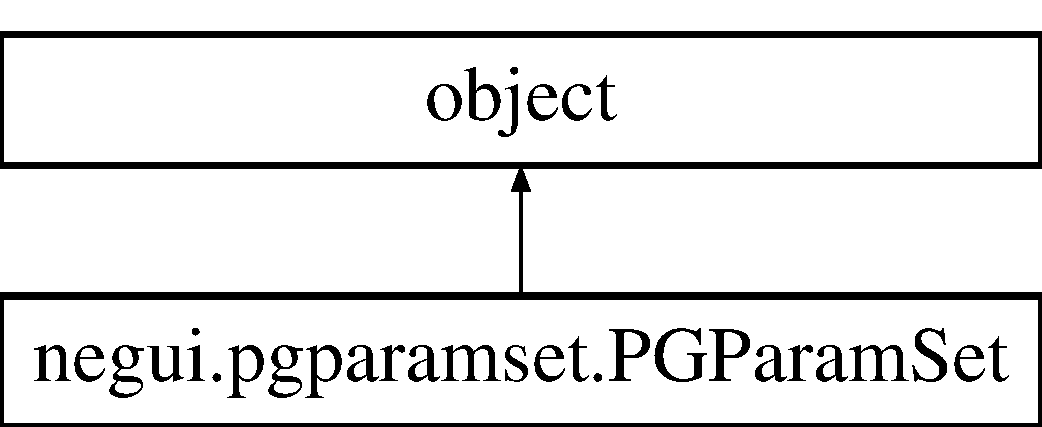
\includegraphics[height=2.000000cm]{classnegui_1_1pgparamset_1_1PGParamSet}
\end{center}
\end{figure}
\subsection*{Public Member Functions}
\begin{DoxyCompactItemize}
\item 
def \hyperlink{classnegui_1_1pgparamset_1_1PGParamSet_a598ea6a166f56fe5be01f86d4d8c91ba}{\+\_\+\+\_\+init\+\_\+\+\_\+} (self, s\+\_\+file\+\_\+with\+\_\+param\+\_\+names=None)
\item 
def {\bfseries get\+Longname\+From\+Tag} (self, s\+\_\+tag)\hypertarget{classnegui_1_1pgparamset_1_1PGParamSet_acc6d8437970d94eed41e05c7bb00d2ca}{}\label{classnegui_1_1pgparamset_1_1PGParamSet_acc6d8437970d94eed41e05c7bb00d2ca}

\item 
def {\bfseries get\+Config\+Section\+Name\+From\+Tag} (self, s\+\_\+tag)\hypertarget{classnegui_1_1pgparamset_1_1PGParamSet_a03c4b8dd0c3728cdcb7bf02ca0e673cb}{}\label{classnegui_1_1pgparamset_1_1PGParamSet_a03c4b8dd0c3728cdcb7bf02ca0e673cb}

\item 
def {\bfseries get\+Default\+Value\+From\+Tag} (self, s\+\_\+tag)\hypertarget{classnegui_1_1pgparamset_1_1PGParamSet_ade081db3140f50468abf16d320b76a12}{}\label{classnegui_1_1pgparamset_1_1PGParamSet_ade081db3140f50468abf16d320b76a12}

\item 
def {\bfseries get\+Section\+Order\+From\+Tag} (self, s\+\_\+tag)\hypertarget{classnegui_1_1pgparamset_1_1PGParamSet_a2bf1131707ba0e0cfa4c2d17e4d76ba4}{}\label{classnegui_1_1pgparamset_1_1PGParamSet_a2bf1131707ba0e0cfa4c2d17e4d76ba4}

\item 
def {\bfseries get\+Section\+Col\+Num\+From\+Tag} (self, s\+\_\+tag)\hypertarget{classnegui_1_1pgparamset_1_1PGParamSet_ae6e2a60dde8d9152b17e7a7d9ecbed59}{}\label{classnegui_1_1pgparamset_1_1PGParamSet_ae6e2a60dde8d9152b17e7a7d9ecbed59}

\item 
def {\bfseries get\+Param\+Order\+Number\+From\+Tag} (self, s\+\_\+tag)\hypertarget{classnegui_1_1pgparamset_1_1PGParamSet_a24d65e7f2a64e79820c04767de1895ca}{}\label{classnegui_1_1pgparamset_1_1PGParamSet_a24d65e7f2a64e79820c04767de1895ca}

\item 
def {\bfseries get\+Tool\+Tip\+From\+Tag} (self, s\+\_\+tag)\hypertarget{classnegui_1_1pgparamset_1_1PGParamSet_afd0f17941dc1e421f299c751266b3bb0}{}\label{classnegui_1_1pgparamset_1_1PGParamSet_afd0f17941dc1e421f299c751266b3bb0}

\item 
def {\bfseries get\+Param\+Type\+From\+Tag} (self, s\+\_\+tag)\hypertarget{classnegui_1_1pgparamset_1_1PGParamSet_a391775e1ec6ef31d6240f354bc695d09}{}\label{classnegui_1_1pgparamset_1_1PGParamSet_a391775e1ec6ef31d6240f354bc695d09}

\item 
def {\bfseries get\+Param\+Min\+From\+Tag} (self, s\+\_\+tag)\hypertarget{classnegui_1_1pgparamset_1_1PGParamSet_a45388124f8b63f1f21a935350022ef17}{}\label{classnegui_1_1pgparamset_1_1PGParamSet_a45388124f8b63f1f21a935350022ef17}

\item 
def {\bfseries get\+Param\+Max\+From\+Tag} (self, s\+\_\+tag)\hypertarget{classnegui_1_1pgparamset_1_1PGParamSet_a90f8f1622c76d72d8d8d6b63e8d14960}{}\label{classnegui_1_1pgparamset_1_1PGParamSet_a90f8f1622c76d72d8d8d6b63e8d14960}

\item 
def {\bfseries get\+G\+U\+I\+Control\+From\+Tag} (self, s\+\_\+tag)\hypertarget{classnegui_1_1pgparamset_1_1PGParamSet_a2e234af54a020c62e1caece36c783fcd}{}\label{classnegui_1_1pgparamset_1_1PGParamSet_a2e234af54a020c62e1caece36c783fcd}

\item 
def {\bfseries get\+Control\+List\+From\+Tag} (self, s\+\_\+tag)\hypertarget{classnegui_1_1pgparamset_1_1PGParamSet_a2811b483838f4655a57e67c4ad3ffa3c}{}\label{classnegui_1_1pgparamset_1_1PGParamSet_a2811b483838f4655a57e67c4ad3ffa3c}

\item 
def {\bfseries get\+Validation\+From\+Tag} (self, s\+\_\+tag)\hypertarget{classnegui_1_1pgparamset_1_1PGParamSet_a205a20b31d36f64c3e722576c9689a66}{}\label{classnegui_1_1pgparamset_1_1PGParamSet_a205a20b31d36f64c3e722576c9689a66}

\item 
def {\bfseries get\+Config\+Section\+Name\+For\+Param} (self, s\+\_\+name)\hypertarget{classnegui_1_1pgparamset_1_1PGParamSet_a4a82ee083106b30250988df78efa89d3}{}\label{classnegui_1_1pgparamset_1_1PGParamSet_a4a82ee083106b30250988df78efa89d3}

\item 
def {\bfseries get\+Default\+Value\+For\+Param} (self, s\+\_\+name)\hypertarget{classnegui_1_1pgparamset_1_1PGParamSet_a41c2137247335135297d3bdf0f7c6dcb}{}\label{classnegui_1_1pgparamset_1_1PGParamSet_a41c2137247335135297d3bdf0f7c6dcb}

\item 
def {\bfseries get\+Section\+Order\+For\+Param} (self, s\+\_\+name)\hypertarget{classnegui_1_1pgparamset_1_1PGParamSet_a18000b825994a6784da5ead88e300e98}{}\label{classnegui_1_1pgparamset_1_1PGParamSet_a18000b825994a6784da5ead88e300e98}

\item 
def {\bfseries get\+Param\+Order\+Number\+For\+Param} (self, s\+\_\+name)\hypertarget{classnegui_1_1pgparamset_1_1PGParamSet_a5eccd6863398ff156943e9f3dd3c2b4c}{}\label{classnegui_1_1pgparamset_1_1PGParamSet_a5eccd6863398ff156943e9f3dd3c2b4c}

\item 
def {\bfseries get\+Section\+Col\+Num\+For\+Param} (self, s\+\_\+name)\hypertarget{classnegui_1_1pgparamset_1_1PGParamSet_aeeeb2bd3d201af38fc265a344412472a}{}\label{classnegui_1_1pgparamset_1_1PGParamSet_aeeeb2bd3d201af38fc265a344412472a}

\item 
def {\bfseries get\+Tool\+Tip\+For\+Param} (self, s\+\_\+name)\hypertarget{classnegui_1_1pgparamset_1_1PGParamSet_af32496fcdac800f7866145183ac5dca1}{}\label{classnegui_1_1pgparamset_1_1PGParamSet_af32496fcdac800f7866145183ac5dca1}

\item 
def {\bfseries get\+Param\+Type\+For\+Param} (self, s\+\_\+name)\hypertarget{classnegui_1_1pgparamset_1_1PGParamSet_a9ae06c3fcb53ba89465abe2cb6df33ce}{}\label{classnegui_1_1pgparamset_1_1PGParamSet_a9ae06c3fcb53ba89465abe2cb6df33ce}

\item 
def {\bfseries get\+Param\+Min\+For\+Param} (self, s\+\_\+name)\hypertarget{classnegui_1_1pgparamset_1_1PGParamSet_a30d903122daa7dca3d8e0d1953d8b10b}{}\label{classnegui_1_1pgparamset_1_1PGParamSet_a30d903122daa7dca3d8e0d1953d8b10b}

\item 
def {\bfseries get\+Param\+Max\+For\+Param} (self, s\+\_\+name)\hypertarget{classnegui_1_1pgparamset_1_1PGParamSet_a2e0c67c114e666cd16574fb6def84f06}{}\label{classnegui_1_1pgparamset_1_1PGParamSet_a2e0c67c114e666cd16574fb6def84f06}

\item 
def {\bfseries get\+G\+U\+I\+Control\+For\+Param} (self, s\+\_\+name)\hypertarget{classnegui_1_1pgparamset_1_1PGParamSet_ae3e401b0a326f3d1c9761123c75953bd}{}\label{classnegui_1_1pgparamset_1_1PGParamSet_ae3e401b0a326f3d1c9761123c75953bd}

\item 
def {\bfseries get\+Control\+List\+For\+Param} (self, s\+\_\+name)\hypertarget{classnegui_1_1pgparamset_1_1PGParamSet_a38a483a791bd4ce9e8284f4c2a578f92}{}\label{classnegui_1_1pgparamset_1_1PGParamSet_a38a483a791bd4ce9e8284f4c2a578f92}

\item 
def {\bfseries get\+Longname\+For\+Param} (self, s\+\_\+name)\hypertarget{classnegui_1_1pgparamset_1_1PGParamSet_a4e6b1c2c38ed89404aefcaa95c1ae8e3}{}\label{classnegui_1_1pgparamset_1_1PGParamSet_a4e6b1c2c38ed89404aefcaa95c1ae8e3}

\item 
def {\bfseries get\+Validation\+For\+Param} (self, s\+\_\+name)\hypertarget{classnegui_1_1pgparamset_1_1PGParamSet_a551326a24cfdff0bc6e0d7dd18c70757}{}\label{classnegui_1_1pgparamset_1_1PGParamSet_a551326a24cfdff0bc6e0d7dd18c70757}

\item 
def \hyperlink{classnegui_1_1pgparamset_1_1PGParamSet_aef97e7ee992a99258a6bbd7b7bf7c5fe}{tag} (self, s\+\_\+name)
\item 
def {\bfseries init\+From\+File} (self, s\+\_\+param\+\_\+name\+\_\+file)\hypertarget{classnegui_1_1pgparamset_1_1PGParamSet_a0d0286ee3d7b8a845db793ca9a299efc}{}\label{classnegui_1_1pgparamset_1_1PGParamSet_a0d0286ee3d7b8a845db793ca9a299efc}

\item 
def {\bfseries param\+\_\+names\+\_\+file} (self)\hypertarget{classnegui_1_1pgparamset_1_1PGParamSet_a8d8478fc187d4c04e3a3c1093f7834be}{}\label{classnegui_1_1pgparamset_1_1PGParamSet_a8d8478fc187d4c04e3a3c1093f7834be}

\item 
def {\bfseries longnames} (self)\hypertarget{classnegui_1_1pgparamset_1_1PGParamSet_a27bf393c0d8052647b19eac34495f06b}{}\label{classnegui_1_1pgparamset_1_1PGParamSet_a27bf393c0d8052647b19eac34495f06b}

\item 
def {\bfseries shortnames} (self)\hypertarget{classnegui_1_1pgparamset_1_1PGParamSet_a0418157edbb31cc2282210baca66a35d}{}\label{classnegui_1_1pgparamset_1_1PGParamSet_a0418157edbb31cc2282210baca66a35d}

\item 
def \hyperlink{classnegui_1_1pgparamset_1_1PGParamSet_a292c23c3d6349027f5c19eec70ea34f8}{tags} (self)
\item 
def {\bfseries section\+\_\+names} (self)\hypertarget{classnegui_1_1pgparamset_1_1PGParamSet_a7f03eecfcbbb1d478ea53d2864f0fc82}{}\label{classnegui_1_1pgparamset_1_1PGParamSet_a7f03eecfcbbb1d478ea53d2864f0fc82}

\end{DoxyCompactItemize}
\subsection*{Static Public Attributes}
\begin{DoxyCompactItemize}
\item 
string {\bfseries D\+E\+L\+I\+M\+I\+T\+E\+R\+\_\+\+T\+A\+G\+\_\+\+F\+I\+E\+L\+DS} = \char`\"{};\char`\"{}\hypertarget{classnegui_1_1pgparamset_1_1PGParamSet_a40e875db5bb216d88fee5fbce8bf229c}{}\label{classnegui_1_1pgparamset_1_1PGParamSet_a40e875db5bb216d88fee5fbce8bf229c}

\item 
int {\bfseries I\+D\+X\+\_\+\+P\+A\+R\+A\+M\+\_\+\+S\+H\+O\+R\+T\+N\+A\+ME} = 0\hypertarget{classnegui_1_1pgparamset_1_1PGParamSet_a5f0fb3e2685ab478b2cc610ddb3cb4ae}{}\label{classnegui_1_1pgparamset_1_1PGParamSet_a5f0fb3e2685ab478b2cc610ddb3cb4ae}

\item 
int {\bfseries I\+D\+X\+\_\+\+P\+A\+R\+A\+M\+\_\+\+T\+AG} = 1\hypertarget{classnegui_1_1pgparamset_1_1PGParamSet_aafe4650bfa58bd9751cdaa173b910c75}{}\label{classnegui_1_1pgparamset_1_1PGParamSet_aafe4650bfa58bd9751cdaa173b910c75}

\item 
int {\bfseries P\+A\+R\+A\+M\+\_\+\+F\+I\+E\+L\+D\+S\+\_\+\+T\+O\+T\+AL} = 2\hypertarget{classnegui_1_1pgparamset_1_1PGParamSet_aeaf803935c95ef6865aa8bc827290cde}{}\label{classnegui_1_1pgparamset_1_1PGParamSet_aeaf803935c95ef6865aa8bc827290cde}

\item 
int {\bfseries I\+D\+X\+\_\+\+T\+A\+G\+\_\+\+F\+E\+I\+L\+D\+\_\+\+L\+O\+N\+G\+N\+A\+ME} = 0\hypertarget{classnegui_1_1pgparamset_1_1PGParamSet_a8df35573197d7171fbb6c900b6dcb057}{}\label{classnegui_1_1pgparamset_1_1PGParamSet_a8df35573197d7171fbb6c900b6dcb057}

\item 
int {\bfseries I\+D\+X\+\_\+\+T\+A\+G\+\_\+\+F\+I\+E\+L\+D\+\_\+\+C\+O\+N\+F\+I\+G\+\_\+\+S\+E\+C\+T\+I\+ON} = 1\hypertarget{classnegui_1_1pgparamset_1_1PGParamSet_ac9ea8e939528fa5975acdfd6c0184d7b}{}\label{classnegui_1_1pgparamset_1_1PGParamSet_ac9ea8e939528fa5975acdfd6c0184d7b}

\item 
int {\bfseries I\+D\+X\+\_\+\+T\+A\+G\+\_\+\+F\+I\+E\+L\+D\+\_\+\+C\+O\+N\+F\+I\+G\+\_\+\+S\+E\+C\+T\+I\+O\+N\+\_\+\+P\+L\+A\+C\+E\+M\+E\+N\+T\+\_\+\+O\+R\+D\+ER} = 2\hypertarget{classnegui_1_1pgparamset_1_1PGParamSet_ace7214b6af0603080aa2d0ea3dea8ea7}{}\label{classnegui_1_1pgparamset_1_1PGParamSet_ace7214b6af0603080aa2d0ea3dea8ea7}

\item 
int {\bfseries I\+D\+X\+\_\+\+T\+A\+G\+\_\+\+F\+I\+E\+L\+D\+\_\+\+C\+O\+L\+U\+M\+N\+\_\+\+N\+U\+M\+B\+ER} = 3\hypertarget{classnegui_1_1pgparamset_1_1PGParamSet_a5c7895ecbfeefb1c547688bbbd790d6f}{}\label{classnegui_1_1pgparamset_1_1PGParamSet_a5c7895ecbfeefb1c547688bbbd790d6f}

\item 
int {\bfseries I\+D\+X\+\_\+\+T\+A\+G\+\_\+\+F\+I\+E\+L\+D\+\_\+\+P\+A\+R\+A\+M\+\_\+\+O\+R\+D\+ER} = 4\hypertarget{classnegui_1_1pgparamset_1_1PGParamSet_a51d57165381da82574640f89b0f2aecb}{}\label{classnegui_1_1pgparamset_1_1PGParamSet_a51d57165381da82574640f89b0f2aecb}

\item 
int {\bfseries I\+D\+X\+\_\+\+T\+A\+G\+\_\+\+F\+I\+E\+L\+D\+\_\+\+D\+E\+F\+A\+U\+L\+T\+\_\+\+V\+A\+L\+UE} = 5\hypertarget{classnegui_1_1pgparamset_1_1PGParamSet_ae133df1f32a04c7088151186a53af461}{}\label{classnegui_1_1pgparamset_1_1PGParamSet_ae133df1f32a04c7088151186a53af461}

\item 
int {\bfseries I\+D\+X\+\_\+\+T\+A\+G\+\_\+\+F\+I\+E\+L\+D\+\_\+\+P\+A\+R\+A\+M\+\_\+\+T\+Y\+PE} = 6\hypertarget{classnegui_1_1pgparamset_1_1PGParamSet_a026542525f9f02da7db6fa5ea86204fe}{}\label{classnegui_1_1pgparamset_1_1PGParamSet_a026542525f9f02da7db6fa5ea86204fe}

\item 
int {\bfseries I\+D\+X\+\_\+\+T\+A\+G\+\_\+\+F\+I\+E\+L\+D\+\_\+\+M\+I\+N\+\_\+\+V\+A\+L\+UE} = 7\hypertarget{classnegui_1_1pgparamset_1_1PGParamSet_ab182cc3f527e31c261b4875ae91fc012}{}\label{classnegui_1_1pgparamset_1_1PGParamSet_ab182cc3f527e31c261b4875ae91fc012}

\item 
int {\bfseries I\+D\+X\+\_\+\+T\+A\+G\+\_\+\+F\+I\+E\+L\+D\+\_\+\+M\+A\+X\+\_\+\+V\+A\+L\+UE} = 8\hypertarget{classnegui_1_1pgparamset_1_1PGParamSet_a88c95f2519ee9eb057f67cadb54283ab}{}\label{classnegui_1_1pgparamset_1_1PGParamSet_a88c95f2519ee9eb057f67cadb54283ab}

\item 
int {\bfseries I\+D\+X\+\_\+\+T\+A\+G\+\_\+\+F\+I\+E\+L\+D\+\_\+\+T\+O\+O\+L\+\_\+\+T\+IP} = 9\hypertarget{classnegui_1_1pgparamset_1_1PGParamSet_a5c414c29c9750f1bb49cfecee9ace56e}{}\label{classnegui_1_1pgparamset_1_1PGParamSet_a5c414c29c9750f1bb49cfecee9ace56e}

\item 
int {\bfseries I\+D\+X\+\_\+\+T\+A\+G\+\_\+\+F\+I\+E\+L\+D\+\_\+\+G\+U\+I\+\_\+\+C\+O\+N\+T\+R\+OL} = 10\hypertarget{classnegui_1_1pgparamset_1_1PGParamSet_a48de36f5304fadf16ea2dc5aa5f9aa10}{}\label{classnegui_1_1pgparamset_1_1PGParamSet_a48de36f5304fadf16ea2dc5aa5f9aa10}

\item 
int {\bfseries I\+D\+X\+\_\+\+T\+A\+G\+\_\+\+F\+I\+E\+L\+D\+\_\+\+G\+U\+I\+\_\+\+C\+O\+N\+T\+R\+O\+L\+\_\+\+L\+I\+ST} = 11\hypertarget{classnegui_1_1pgparamset_1_1PGParamSet_aee6b6d1c25ba78020df4ee6c4db6b4da}{}\label{classnegui_1_1pgparamset_1_1PGParamSet_aee6b6d1c25ba78020df4ee6c4db6b4da}

\item 
int {\bfseries I\+D\+X\+\_\+\+T\+A\+G\+\_\+\+F\+I\+E\+L\+D\+\_\+\+V\+A\+L\+I\+D\+A\+T\+I\+ON} = 12\hypertarget{classnegui_1_1pgparamset_1_1PGParamSet_a859b19d511c2d6b5b912f9fabe172b10}{}\label{classnegui_1_1pgparamset_1_1PGParamSet_a859b19d511c2d6b5b912f9fabe172b10}

\item 
string {\bfseries C\+O\+M\+M\+E\+N\+T\+\_\+\+C\+H\+AR} = \char`\"{}\#\char`\"{}\hypertarget{classnegui_1_1pgparamset_1_1PGParamSet_a3699c7f57795876fe0a6d4482bfd3295}{}\label{classnegui_1_1pgparamset_1_1PGParamSet_a3699c7f57795876fe0a6d4482bfd3295}

\end{DoxyCompactItemize}


\subsection{Detailed Description}
\begin{DoxyVerb}Class ParamSet is used to replace
parameter names as given by code variables
and associates each with a more user-friendly
name.  These longer, fuller names are used
for example, as labels in the gui interface
that allows users to set the parameters.

2016_09_08
Over last few weeks have added fields to the "tag"
column in the paramset files, read by objects of
this class.  There are now many sub-fields inside
the tag that are used to get a default value, 
type the value, add a tool tip, and give a max
and min value for validation.  See the IDX_ declarations
below for order and meaning of these tag "subfields"

2016_09_24
The longname item has been moved into the tag, so that now
only two columns are given in the paremeter file.\end{DoxyVerb}
 

Definition at line 32 of file pgparamset.\+py.



\subsection{Constructor \& Destructor Documentation}
\index{negui\+::pgparamset\+::\+P\+G\+Param\+Set@{negui\+::pgparamset\+::\+P\+G\+Param\+Set}!\+\_\+\+\_\+init\+\_\+\+\_\+@{\+\_\+\+\_\+init\+\_\+\+\_\+}}
\index{\+\_\+\+\_\+init\+\_\+\+\_\+@{\+\_\+\+\_\+init\+\_\+\+\_\+}!negui\+::pgparamset\+::\+P\+G\+Param\+Set@{negui\+::pgparamset\+::\+P\+G\+Param\+Set}}
\subsubsection[{\texorpdfstring{\+\_\+\+\_\+init\+\_\+\+\_\+(self, s\+\_\+file\+\_\+with\+\_\+param\+\_\+names=\+None)}{__init__(self, s_file_with_param_names=None)}}]{\setlength{\rightskip}{0pt plus 5cm}def negui.\+pgparamset.\+P\+G\+Param\+Set.\+\_\+\+\_\+init\+\_\+\+\_\+ (
\begin{DoxyParamCaption}
\item[{}]{self, }
\item[{}]{s\+\_\+file\+\_\+with\+\_\+param\+\_\+names = {\ttfamily None}}
\end{DoxyParamCaption}
)}\hypertarget{classnegui_1_1pgparamset_1_1PGParamSet_a598ea6a166f56fe5be01f86d4d8c91ba}{}\label{classnegui_1_1pgparamset_1_1PGParamSet_a598ea6a166f56fe5be01f86d4d8c91ba}
\begin{DoxyVerb}If provided, arg s_file_with_param_names
should be a file with 2 or more strings on each line,
tab-separated, the first value giving the short
name of the parameter, the second the long (full)
name, the third (if present)
\end{DoxyVerb}
 

Definition at line 147 of file pgparamset.\+py.


\begin{DoxyCode}
147     \textcolor{keyword}{def }\hyperlink{classnegui_1_1pgparamset_1_1PGParamSet_a598ea6a166f56fe5be01f86d4d8c91ba}{\_\_init\_\_}( self, s\_file\_with\_param\_names = None ):
148 
149         \textcolor{stringliteral}{'''}
150 \textcolor{stringliteral}{        If provided, arg s\_file\_with\_param\_names}
151 \textcolor{stringliteral}{        should be a file with 2 or more strings on each line,}
152 \textcolor{stringliteral}{        tab-separated, the first value giving the short}
153 \textcolor{stringliteral}{        name of the parameter, the second the long (full)}
154 \textcolor{stringliteral}{        name, the third (if present)}
155 \textcolor{stringliteral}{        '''}
156         self.\hyperlink{classnegui_1_1pgparamset_1_1PGParamSet_aafa67026a09aa523151728cba95e0d6d}{\_\_file\_with\_param\_names}=s\_file\_with\_param\_names
157         self.\hyperlink{classnegui_1_1pgparamset_1_1PGParamSet_aa13eaff9049bc16fa4090c8b85915f3c}{\_\_tags\_by\_shortname}=\{\}
158 
159         \textcolor{keywordflow}{if} s\_file\_with\_param\_names \textcolor{keywordflow}{is} \textcolor{keywordflow}{not} \textcolor{keywordtype}{None}:
160             self.\hyperlink{classnegui_1_1pgparamset_1_1PGParamSet_abc19f133ab3ecc86ec8099549b0b45bb}{\_\_init\_from\_file}( s\_file\_with\_param\_names )
161         \textcolor{comment}{#end if file name given}
162         \textcolor{keywordflow}{return}
\end{DoxyCode}


\subsection{Member Function Documentation}
\index{negui\+::pgparamset\+::\+P\+G\+Param\+Set@{negui\+::pgparamset\+::\+P\+G\+Param\+Set}!tag@{tag}}
\index{tag@{tag}!negui\+::pgparamset\+::\+P\+G\+Param\+Set@{negui\+::pgparamset\+::\+P\+G\+Param\+Set}}
\subsubsection[{\texorpdfstring{tag(self, s\+\_\+name)}{tag(self, s_name)}}]{\setlength{\rightskip}{0pt plus 5cm}def negui.\+pgparamset.\+P\+G\+Param\+Set.\+tag (
\begin{DoxyParamCaption}
\item[{}]{self, }
\item[{}]{s\+\_\+name}
\end{DoxyParamCaption}
)}\hypertarget{classnegui_1_1pgparamset_1_1PGParamSet_aef97e7ee992a99258a6bbd7b7bf7c5fe}{}\label{classnegui_1_1pgparamset_1_1PGParamSet_aef97e7ee992a99258a6bbd7b7bf7c5fe}
\begin{DoxyVerb}param s_name can be either among the 
short or long names (or both). Shortnames
are checked first.  First instance of name
provides its tag as the return value.
\end{DoxyVerb}
 

Definition at line 391 of file pgparamset.\+py.


\begin{DoxyCode}
391     \textcolor{keyword}{def }\hyperlink{classnegui_1_1pgparamset_1_1PGParamSet_aef97e7ee992a99258a6bbd7b7bf7c5fe}{tag}( self, s\_name ):
392         \textcolor{stringliteral}{'''}
393 \textcolor{stringliteral}{        param s\_name can be either among the }
394 \textcolor{stringliteral}{        short or long names (or both). Shortnames}
395 \textcolor{stringliteral}{        are checked first.  First instance of name}
396 \textcolor{stringliteral}{        provides its tag as the return value.}
397 \textcolor{stringliteral}{        '''}
398         s\_val=\textcolor{keywordtype}{None}
399 
400         \textcolor{keywordflow}{if} s\_name \textcolor{keywordflow}{in} self.\hyperlink{classnegui_1_1pgparamset_1_1PGParamSet_aa13eaff9049bc16fa4090c8b85915f3c}{\_\_tags\_by\_shortname}:
401             s\_val = self.\hyperlink{classnegui_1_1pgparamset_1_1PGParamSet_aa13eaff9049bc16fa4090c8b85915f3c}{\_\_tags\_by\_shortname}[ s\_name ]
402         \textcolor{keywordflow}{else}:
403             s\_msg=\textcolor{stringliteral}{"In PGParamSet instance, def tag(), no tag "} \(\backslash\)
404                     + \textcolor{stringliteral}{"associated with "} \(\backslash\)
405                     + \textcolor{stringliteral}{"param name, "} + s\_name + \textcolor{stringliteral}{"."}
406             \textcolor{keywordflow}{raise} Exception ( s\_msg )
407         \textcolor{comment}{#end if tag in short else if tag in long}
408 
409         \textcolor{keywordflow}{return} s\_val
\end{DoxyCode}
\index{negui\+::pgparamset\+::\+P\+G\+Param\+Set@{negui\+::pgparamset\+::\+P\+G\+Param\+Set}!tags@{tags}}
\index{tags@{tags}!negui\+::pgparamset\+::\+P\+G\+Param\+Set@{negui\+::pgparamset\+::\+P\+G\+Param\+Set}}
\subsubsection[{\texorpdfstring{tags(self)}{tags(self)}}]{\setlength{\rightskip}{0pt plus 5cm}def negui.\+pgparamset.\+P\+G\+Param\+Set.\+tags (
\begin{DoxyParamCaption}
\item[{}]{self}
\end{DoxyParamCaption}
)}\hypertarget{classnegui_1_1pgparamset_1_1PGParamSet_a292c23c3d6349027f5c19eec70ea34f8}{}\label{classnegui_1_1pgparamset_1_1PGParamSet_a292c23c3d6349027f5c19eec70ea34f8}
\begin{DoxyVerb}returns a list of tags, without their associated
param names (short or long).  Useful to get
the set of unique tags if the tags categorize
the paramset into groups
\end{DoxyVerb}
 

Definition at line 460 of file pgparamset.\+py.


\begin{DoxyCode}
460     \textcolor{keyword}{def }\hyperlink{classnegui_1_1pgparamset_1_1PGParamSet_a292c23c3d6349027f5c19eec70ea34f8}{tags}(self):
461         \textcolor{stringliteral}{'''}
462 \textcolor{stringliteral}{        returns a list of tags, without their associated}
463 \textcolor{stringliteral}{        param names (short or long).  Useful to get}
464 \textcolor{stringliteral}{        the set of unique tags if the tags categorize}
465 \textcolor{stringliteral}{        the paramset into groups}
466 \textcolor{stringliteral}{        '''}
467         ls\_tags=self.\_\_tags\_by\_shortname.values()
468         ls\_tags.sort()
469         \textcolor{keywordflow}{return} ls\_tags
\end{DoxyCode}


The documentation for this class was generated from the following file\+:\begin{DoxyCompactItemize}
\item 
pgparamset.\+py\end{DoxyCompactItemize}

\hypertarget{classnegui_1_1pgsimupopresources_1_1PGSimuPopResources}{}\section{negui.\+pgsimupopresources.\+P\+G\+Simu\+Pop\+Resources Class Reference}
\label{classnegui_1_1pgsimupopresources_1_1PGSimuPopResources}\index{negui.\+pgsimupopresources.\+P\+G\+Simu\+Pop\+Resources@{negui.\+pgsimupopresources.\+P\+G\+Simu\+Pop\+Resources}}
Inheritance diagram for negui.\+pgsimupopresources.\+P\+G\+Simu\+Pop\+Resources\+:\begin{figure}[H]
\begin{center}
\leavevmode
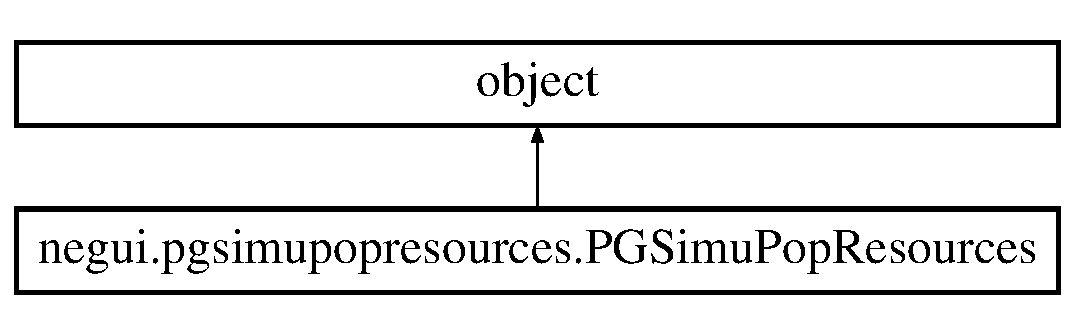
\includegraphics[height=2.000000cm]{classnegui_1_1pgsimupopresources_1_1PGSimuPopResources}
\end{center}
\end{figure}
\subsection*{Public Member Functions}
\begin{DoxyCompactItemize}
\item 
def \hyperlink{classnegui_1_1pgsimupopresources_1_1PGSimuPopResources_a8e79c3f4c6c291a606c9f0c2f259a293}{\+\_\+\+\_\+init\+\_\+\+\_\+} (self, ls\+\_\+life\+\_\+table\+\_\+files, b\+\_\+write\+\_\+warnings=False)
\item 
def \hyperlink{classnegui_1_1pgsimupopresources_1_1PGSimuPopResources_a37fa2c7b4da84a2281231943a8e61c6c}{get\+Life\+Table\+Value} (self, s\+\_\+model\+\_\+name, s\+\_\+section, s\+\_\+option)
\item 
def {\bfseries life\+\_\+table\+\_\+files} (self)\hypertarget{classnegui_1_1pgsimupopresources_1_1PGSimuPopResources_a7f5ebba41ad2c1e20e3d31016b46e630}{}\label{classnegui_1_1pgsimupopresources_1_1PGSimuPopResources_a7f5ebba41ad2c1e20e3d31016b46e630}

\end{DoxyCompactItemize}


\subsection{Detailed Description}
\begin{DoxyVerb}\end{DoxyVerb}
 

Definition at line 26 of file pgsimupopresources.\+py.



\subsection{Constructor \& Destructor Documentation}
\index{negui\+::pgsimupopresources\+::\+P\+G\+Simu\+Pop\+Resources@{negui\+::pgsimupopresources\+::\+P\+G\+Simu\+Pop\+Resources}!\+\_\+\+\_\+init\+\_\+\+\_\+@{\+\_\+\+\_\+init\+\_\+\+\_\+}}
\index{\+\_\+\+\_\+init\+\_\+\+\_\+@{\+\_\+\+\_\+init\+\_\+\+\_\+}!negui\+::pgsimupopresources\+::\+P\+G\+Simu\+Pop\+Resources@{negui\+::pgsimupopresources\+::\+P\+G\+Simu\+Pop\+Resources}}
\subsubsection[{\texorpdfstring{\+\_\+\+\_\+init\+\_\+\+\_\+(self, ls\+\_\+life\+\_\+table\+\_\+files, b\+\_\+write\+\_\+warnings=\+False)}{__init__(self, ls_life_table_files, b_write_warnings=False)}}]{\setlength{\rightskip}{0pt plus 5cm}def negui.\+pgsimupopresources.\+P\+G\+Simu\+Pop\+Resources.\+\_\+\+\_\+init\+\_\+\+\_\+ (
\begin{DoxyParamCaption}
\item[{}]{self, }
\item[{}]{ls\+\_\+life\+\_\+table\+\_\+files, }
\item[{}]{b\+\_\+write\+\_\+warnings = {\ttfamily False}}
\end{DoxyParamCaption}
)}\hypertarget{classnegui_1_1pgsimupopresources_1_1PGSimuPopResources_a8e79c3f4c6c291a606c9f0c2f259a293}{}\label{classnegui_1_1pgsimupopresources_1_1PGSimuPopResources_a8e79c3f4c6c291a606c9f0c2f259a293}
\begin{DoxyVerb}Param ls_life_table_files is a list of configuration file names,
    with table info, such as survivial and fecundity rates,
    gamma values, and ages.
Param b_write_warnings is a flag. If true warnigs are written to stderr.\end{DoxyVerb}
 

Definition at line 30 of file pgsimupopresources.\+py.


\begin{DoxyCode}
30     \textcolor{keyword}{def }\hyperlink{classnegui_1_1pgsimupopresources_1_1PGSimuPopResources_a8e79c3f4c6c291a606c9f0c2f259a293}{\_\_init\_\_}( self, ls\_life\_table\_files, b\_write\_warnings=False ):
31         \textcolor{stringliteral}{'''}
32 \textcolor{stringliteral}{        Param ls\_life\_table\_files is a list of configuration file names,}
33 \textcolor{stringliteral}{            with table info, such as survivial and fecundity rates,}
34 \textcolor{stringliteral}{            gamma values, and ages.}
35 \textcolor{stringliteral}{        Param b\_write\_warnings is a flag. If true warnigs are written to stderr.}
36 \textcolor{stringliteral}{        }
37 \textcolor{stringliteral}{        '''}
38         self.\hyperlink{classnegui_1_1pgsimupopresources_1_1PGSimuPopResources_a70ffb8eb62a843aec8f42e337c81fc3b}{\_\_life\_table\_files}=ls\_life\_table\_files
39         self.\hyperlink{classnegui_1_1pgsimupopresources_1_1PGSimuPopResources_ae4805ab6ba55817bc2e40fd622d76483}{\_\_write\_warnings}=b\_write\_warnings
40         self.\hyperlink{classnegui_1_1pgsimupopresources_1_1PGSimuPopResources_ae32ca7cc4b6a1563734a82da0a0c6608}{\_\_lifetables}=\{\}
41         self.\hyperlink{classnegui_1_1pgsimupopresources_1_1PGSimuPopResources_aed06da70af5eea2be1c6caabf35032af}{\_\_get\_life\_tables}( ls\_life\_table\_files )
42 
43         \textcolor{keywordflow}{return}
\end{DoxyCode}


\subsection{Member Function Documentation}
\index{negui\+::pgsimupopresources\+::\+P\+G\+Simu\+Pop\+Resources@{negui\+::pgsimupopresources\+::\+P\+G\+Simu\+Pop\+Resources}!get\+Life\+Table\+Value@{get\+Life\+Table\+Value}}
\index{get\+Life\+Table\+Value@{get\+Life\+Table\+Value}!negui\+::pgsimupopresources\+::\+P\+G\+Simu\+Pop\+Resources@{negui\+::pgsimupopresources\+::\+P\+G\+Simu\+Pop\+Resources}}
\subsubsection[{\texorpdfstring{get\+Life\+Table\+Value(self, s\+\_\+model\+\_\+name, s\+\_\+section, s\+\_\+option)}{getLifeTableValue(self, s_model_name, s_section, s_option)}}]{\setlength{\rightskip}{0pt plus 5cm}def negui.\+pgsimupopresources.\+P\+G\+Simu\+Pop\+Resources.\+get\+Life\+Table\+Value (
\begin{DoxyParamCaption}
\item[{}]{self, }
\item[{}]{s\+\_\+model\+\_\+name, }
\item[{}]{s\+\_\+section, }
\item[{}]{s\+\_\+option}
\end{DoxyParamCaption}
)}\hypertarget{classnegui_1_1pgsimupopresources_1_1PGSimuPopResources_a37fa2c7b4da84a2281231943a8e61c6c}{}\label{classnegui_1_1pgsimupopresources_1_1PGSimuPopResources_a37fa2c7b4da84a2281231943a8e61c6c}
\begin{DoxyVerb}Tries to fetch the value, 
Returns a None instance if any of 
the parameter values are not found.

On fail also records the first level
that was not found, and
if flag self.__write_warnings
is true, reports the failure to
stderr.
\end{DoxyVerb}
 

Definition at line 77 of file pgsimupopresources.\+py.


\begin{DoxyCode}
77     \textcolor{keyword}{def }\hyperlink{classnegui_1_1pgsimupopresources_1_1PGSimuPopResources_a37fa2c7b4da84a2281231943a8e61c6c}{getLifeTableValue}( self, s\_model\_name, s\_section, s\_option ):
78         \textcolor{stringliteral}{"""}
79 \textcolor{stringliteral}{        Tries to fetch the value, }
80 \textcolor{stringliteral}{        Returns a None instance if any of }
81 \textcolor{stringliteral}{        the parameter values are not found.}
82 \textcolor{stringliteral}{}
83 \textcolor{stringliteral}{        On fail also records the first level}
84 \textcolor{stringliteral}{        that was not found, and}
85 \textcolor{stringliteral}{        if flag self.\_\_write\_warnings}
86 \textcolor{stringliteral}{        is true, reports the failure to}
87 \textcolor{stringliteral}{        stderr.}
88 \textcolor{stringliteral}{        """}
89 
90         v\_value=\textcolor{keywordtype}{None}
91         s\_warning=\textcolor{keywordtype}{None}
92 
93         \textcolor{keywordflow}{try}:
94             o\_parser=self.\hyperlink{classnegui_1_1pgsimupopresources_1_1PGSimuPopResources_ae32ca7cc4b6a1563734a82da0a0c6608}{\_\_lifetables}[ s\_model\_name ]
95             v\_value=o\_parser.get( s\_section, s\_option )
96         \textcolor{keywordflow}{except} KeyError \textcolor{keyword}{as} ke:
97 
98             s\_warnings= \textcolor{stringliteral}{"Warning: In PGSimuPopResources instance, def getLifeTableValue, "} \(\backslash\)
99                     + \textcolor{stringliteral}{"no life table found for model: "}  \(\backslash\)
100                     + s\_model\_name + \textcolor{stringliteral}{"\(\backslash\)n"} 
101 
102         \textcolor{keywordflow}{except} NoSectionError \textcolor{keyword}{as} nse:
103 
104             s\_warning=\textcolor{stringliteral}{"Warning: In PGSimuPopResources instance, def getLifeTableValue, "} \(\backslash\)
105                     + \textcolor{stringliteral}{"no section in life table for model: "}  \(\backslash\)
106                     + s\_model\_name + \textcolor{stringliteral}{"section: "} + s\_section + \textcolor{stringliteral}{"\(\backslash\)n"} 
107 
108         \textcolor{keywordflow}{except} NoOptionError \textcolor{keyword}{as} noe:
109 
110             s\_warning= \textcolor{stringliteral}{"Warning: In PGSimuPopResources instance, def getLifeTableValue, "} \(\backslash\)
111                     + \textcolor{stringliteral}{"no option in life table for model: "}  \(\backslash\)
112                     + s\_model\_name + \textcolor{stringliteral}{"section: "} + s\_section + \textcolor{stringliteral}{"option: "} \(\backslash\)
113                     + s\_option + \textcolor{stringliteral}{"\(\backslash\)n"} 
114         \textcolor{comment}{#end try, except, except, except}
115 
116         \textcolor{keywordflow}{if} self.\hyperlink{classnegui_1_1pgsimupopresources_1_1PGSimuPopResources_ae4805ab6ba55817bc2e40fd622d76483}{\_\_write\_warnings} \textcolor{keywordflow}{and} s\_warning \textcolor{keywordflow}{is} \textcolor{keywordflow}{not} \textcolor{keywordtype}{None}:
117             sys.stderr.write( s\_warning )
118         \textcolor{comment}{#end if write warnings }
119 
120         \textcolor{comment}{#eval will throw a type error if v\_value is None}
121         \textcolor{keywordflow}{return} eval( v\_value ) \textcolor{keywordflow}{if} v\_value \textcolor{keywordflow}{is} \textcolor{keywordflow}{not} \textcolor{keywordtype}{None} \textcolor{keywordflow}{else} \textcolor{keywordtype}{None}
122 
\end{DoxyCode}


The documentation for this class was generated from the following file\+:\begin{DoxyCompactItemize}
\item 
pgsimupopresources.\+py\end{DoxyCompactItemize}

%--- End generated contents ---

% Index
\backmatter
\newpage
\phantomsection
\clearemptydoublepage
\addcontentsline{toc}{chapter}{Index}
\printindex

\end{document}
